\documentclass[10pt,a4paper]{article}
\usepackage[T1]{fontenc}
\usepackage[utf8]{inputenc}
\usepackage{lmodern}
\renewcommand{\familydefault}{\sfdefault}
\usepackage[margin=12mm,headheight=16pt,headsep=4mm,footskip=6mm]{geometry}
\usepackage{colortbl}
\usepackage{graphicx,xcolor,amsmath,amssymb,array,longtable,booktabs,ragged2e,enumitem,fancyhdr,needspace,caption,multicol}
\usepackage{tcolorbox}
\tcbuselibrary{breakable}
\usepackage{fvextra}
\usepackage{hyperref,xurl}
\definecolor{navy}{HTML}{16324A}
\definecolor{teal}{HTML}{176B66}
\definecolor{amber}{HTML}{9C5D11}
\definecolor{danger}{HTML}{9D3538}
\definecolor{ice}{HTML}{EDF3F8}
\definecolor{mint}{HTML}{EEF6F2}
\definecolor{sand}{HTML}{FFF5E5}
\definecolor{line}{HTML}{CCD7DF}
\hypersetup{colorlinks=true,linkcolor=navy,urlcolor=teal,pdftitle={SC2006 A4 Visual Examination Reference},pdfauthor={Study reference; unofficial worked answers},bookmarksnumbered=false}
\setlength{\columnsep}{6mm}
\setlength{\columnseprule}{.2pt}
\def\columnseprulecolor{\color{line}}
\setlength{\multicolsep}{5pt}
\newenvironment{studycolumns}{\begin{multicols}{2}\raggedcolumns}{\end{multicols}}
\newenvironment{referenceentries}{\par\begingroup\fontsize{9}{11}\selectfont}{\par\endgroup}
\setlength{\parindent}{0pt}
\setlength{\parskip}{3pt}
\setlength{\emergencystretch}{2em}
\setlength{\LTpre}{3pt}
\setlength{\LTpost}{4pt}
\setlength{\tabcolsep}{4pt}
\renewcommand{\arraystretch}{1.12}
\setlist{nosep,leftmargin=1.6em,topsep=3pt,itemsep=2pt,parsep=1pt}
\setlist[enumerate,2]{label=\alph*.,leftmargin=1.7em}
\newcolumntype{L}[1]{>{\RaggedRight\arraybackslash}p{#1}}
\captionsetup{font=footnotesize,labelfont=bf,skip=2pt}
\newtcolorbox{eli5box}{breakable,colback=ice,colframe=navy,boxrule=.5pt,arc=1mm,left=2mm,right=2mm,top=1mm,bottom=1mm,title=ELI5,fonttitle=\bfseries,colbacktitle=navy,coltitle=white}
\newtcolorbox{watchbox}{breakable,colback=sand,colframe=amber,boxrule=.5pt,arc=1mm,left=2mm,right=2mm,top=1mm,bottom=1mm,title=Traps and things to check,fonttitle=\bfseries,colbacktitle=amber,coltitle=white}
\newtcolorbox{examlinkbox}{breakable,colback=mint,colframe=teal,boxrule=.4pt,arc=1mm,left=2mm,right=2mm,top=1mm,bottom=1mm,title=Where it helps in the papers,fonttitle=\bfseries,colbacktitle=teal,coltitle=white}
\DefineVerbatimEnvironment{ReferenceCode}{Verbatim}{breaklines=true,breakanywhere=true,fontsize=\small,frame=lines,framesep=2mm,rulecolor=\color{line}}
\newcommand{\code}[1]{\texttt{#1}}
\newcommand{\chapteropen}[2]{\par\Needspace{160pt}\bigskip\phantomsection\addcontentsline{toc}{section}{#1}\markboth{#1}{#1}\section*{#1}\label{#2}}
\newcommand{\sectionlabel}[1]{\phantomsection\label{#1}}
\pagestyle{fancy}
\fancyhf{}
\fancyhead[L]{\footnotesize\textcolor{navy}{SC2006\;|\;Visual examination reference}}
\fancyhead[R]{\footnotesize\textcolor{navy}{\nouppercase{\leftmark}}}
\fancyfoot[L]{\scriptsize SC2006 visual reference}
\fancyfoot[R]{\scriptsize\thepage}
\renewcommand{\headrulewidth}{.3pt}
\renewcommand{\footrulewidth}{.2pt}
\setcounter{tocdepth}{1}
\raggedbottom

\begin{document}
\markboth{Navigation}{}
{\color{navy}\fontsize{20}{23}\selectfont\bfseries SC2006 Visual examination reference\par}
{\small A4 chapter guide, four older papers grouped by question type and four recent worked papers. Revised 4 November 2026.}\par
\textbf{Use:} read the ELI5 introduction, inspect the diagram, then use the rules and traps to build a case-specific answer. Tutorial material already covered in lecture chapters appears once.
\par\textbf{Historical format:} all eight supplied papers allow two hours for four compulsory 25-mark questions.
\begin{longtable}{L{.12\linewidth}L{.52\linewidth}L{.28\linewidth}}
\toprule\rowcolor{ice}\textbf{Question} & \textbf{What to find first} & \textbf{Chapter / page}\\\midrule\endhead
Q1 & Actors, goals, use-case relationships and behaviour; one paper adds stakeholders/requirements. & Ch. 2--3, pp.\ \pageref{chapter-2}--\pageref{chapter-3}\\
Q2 & Conceptual classes, state/activity/dialog diagrams, development process and Scrum reasoning. & Ch. 4--5, 7--8; pp.\ \pageref{chapter-4}, \pageref{chapter-5}, \pageref{chapter-7}, \pageref{chapter-8}\\
Q3 & Architecture tied to the case, NFRs, design-pattern roles, trade-offs and responsibility/LLM questions. & Ch. 9--11, 16; pp.\ \pageref{chapter-9}, \pageref{chapter-10}, \pageref{chapter-11}, \pageref{chapter-16}\\
Q4 & ECs, full boundary triplets, one-invalid defensive rows and expected outcomes; testing/maintenance extensions. & Ch. 12--13, 16; pp.\ \pageref{chapter-12}, \pageref{chapter-13}, \pageref{chapter-16}\\
\bottomrule
\end{longtable}
\textbf{Print:} A4, actual size, one page per sheet side. All pages are portrait. Colour labels remain readable in greyscale.
\par\textbf{Status:} worked answers are unofficial; assumptions are labelled. Use original PDFs for exact questions and proper UML notation in examination drawings. Historical formats do not guarantee the next paper.
\begingroup\small
\setlength{\parskip}{0pt}
\makeatletter\renewcommand{\l@section}{\@dottedtocline{1}{0pt}{1.5em}}\makeatother
\tableofcontents
\endgroup
\clearpage
\chapteropen{Chapter 1: Software engineering and the SDLC}{chapter-1}
\markboth{Ch. 1 | SDLC}{}


\begin{studycolumns}
\vspace{0pt}
\begin{eli5box}
Building software is like building a playground. First ask who needs it and what they need; then draw plans, choose the structure, build it, check it and keep repairing it. The drawings and checklists are work products. A process explains how the team revisits those activities, not merely a row of boxes.
\end{eli5box}
\textbf{Answer check:} Trace the case from requirement to model, design and test. Process models arrange activities; architectures arrange components; patterns solve recurring design problems. Test design starts before execution.


\needspace{289pt}
\par\smallskip\noindent\begin{minipage}{\linewidth}\centering
\begin{minipage}[t]{0.488\linewidth}\centering\scriptsize\textbf{1}\par\smallskip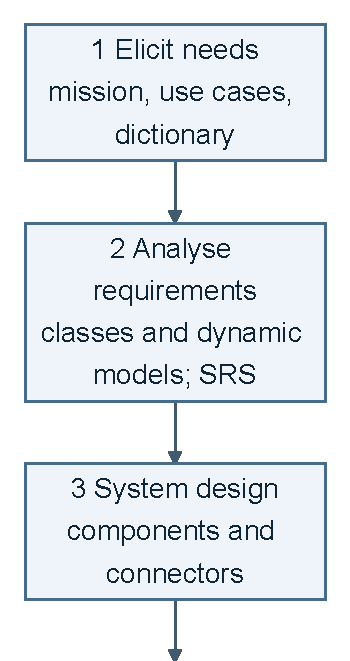
\includegraphics[width=103.04pt]{images/fig-001-compact-1.pdf}\end{minipage}\hfill
\begin{minipage}[t]{0.488\linewidth}\centering\scriptsize\textbf{2}\par\smallskip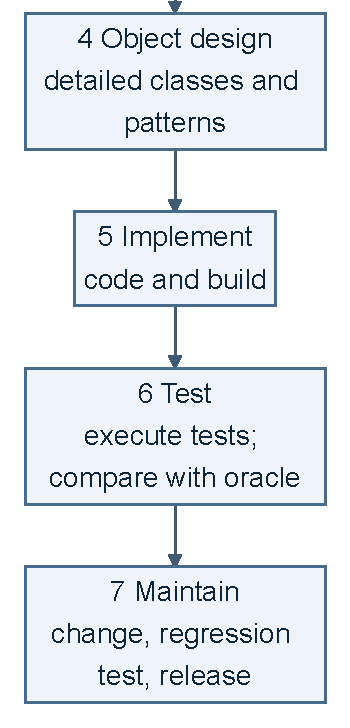
\includegraphics[width=103.04pt]{images/fig-001-compact-2.pdf}\end{minipage}
\captionof{figure}{1. The spine of the course: SDLC \ensuremath{\rightarrow} artefacts --- follow numbered panels; crossing arrows continue.}\end{minipage}\par\smallskip


\needspace{4\baselineskip}
\subsection*{Milestones and work products (L1 work-product table)}
\sectionlabel{h-milestones-and-work-products-l1-work-product-table}

\begin{referenceentries}
\textit{\textbf{Phase} / \textbf{Work products /\allowbreak{} milestones}}\par\smallskip
\noindent \textbf{Requirements specification}: SRS, prototype, requirements review\par
\noindent \textbf{Design}: Software Design Document, Interface Design Document, models, \textbf{test cases}; preliminary \& final design reviews\par
\noindent \textbf{Implementation}: Source code, system build, technical documentation, user manual\par
\noindent \textbf{Testing}: Test execution, test report, user acceptance test\par
\noindent \textbf{Maintenance}: Change request, bug report, patch release, upgrade\par
\end{referenceentries}
\needspace{4\baselineskip}
\subsection*{Definition to memorise}
\sectionlabel{h-definition-to-memorise}

\begin{quote}\small\color{navy}
\textbf{Software engineering} is \emph{the production of maintainable, fault-free software that meets the user's requirements and is delivered on time and within budget.}

\end{quote}


\needspace{4\baselineskip}
\subsection*{The four process activities (also the exam-safe summary)}
\sectionlabel{h-the-four-process-activities-also-the-exam-safe-summary}
\textbf{Specification} (what it should do) \ensuremath{\rightarrow} \textbf{Design \& implementation} (organisation + code) \ensuremath{\rightarrow} \textbf{Validation} (does it do what the customer wants) \ensuremath{\rightarrow} \textbf{Evolution} (change in response to need).


\begin{quote}\small\color{navy}
\textbf{Trap:} process models arrange SDLC activities; architectures arrange components/connectors; design patterns solve recurring object-collaboration problems.

\end{quote}
\end{studycolumns}

\subsection*{Requirement \ensuremath{\rightarrow} analysis \ensuremath{\rightarrow} design traceability chain}
\sectionlabel{h-requirement--analysis--design-traceability-chain}


\par\smallskip\noindent\begin{minipage}{\linewidth}\centering
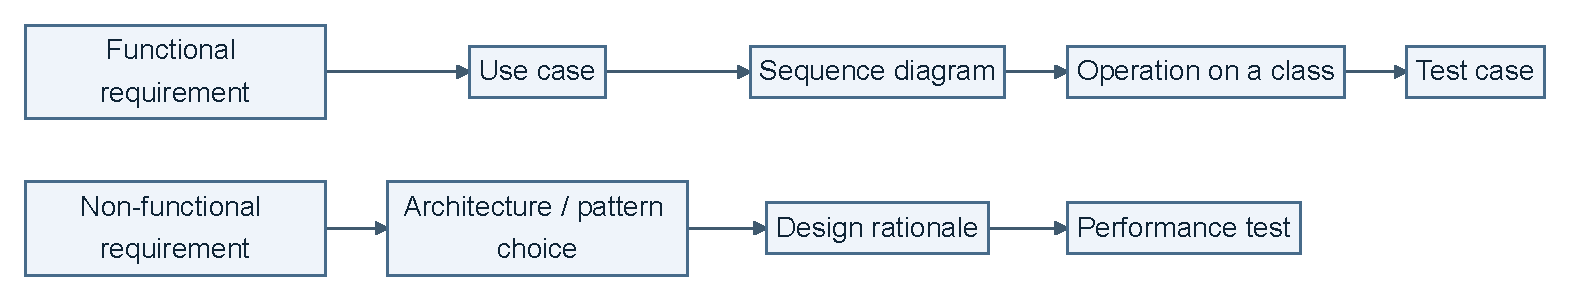
\includegraphics[width=462.30pt]{images/fig-002.pdf}
\captionof{figure}{Requirement \ensuremath{\rightarrow} analysis \ensuremath{\rightarrow} design traceability chain}\end{minipage}\par\smallskip




\chapteropen{Chapter 2: Requirements elicitation}{chapter-2}
\markboth{Ch. 2 | Requirements}{}


\begin{studycolumns}
\vspace{0pt}
\begin{eli5box}
A customer saying 'make a great bicycle' is not yet a testable order. Ask who rides it, where, what it must do and how you will know it is good enough. 'Has brakes' is a capability; 'stops within an agreed distance under stated conditions' is a quality target.
\end{eli5box}
\textbf{Answer check:} Identify stakeholders, atomise requirements, attach measurable acceptance conditions and mark missing policy TBD. Security-related actions can be FRs; a digit alone does not make an NFR.
\needspace{4\baselineskip}
\subsection*{Visual: classify a requirement}
\sectionlabel{h-visual-classify-a-requirement}
Read what the statement asserts, then check whether you can verify it.
\end{studycolumns}


\par\smallskip\noindent\begin{minipage}{\linewidth}\centering
\begin{minipage}[t]{0.488\linewidth}\centering\scriptsize\textbf{1}\par\smallskip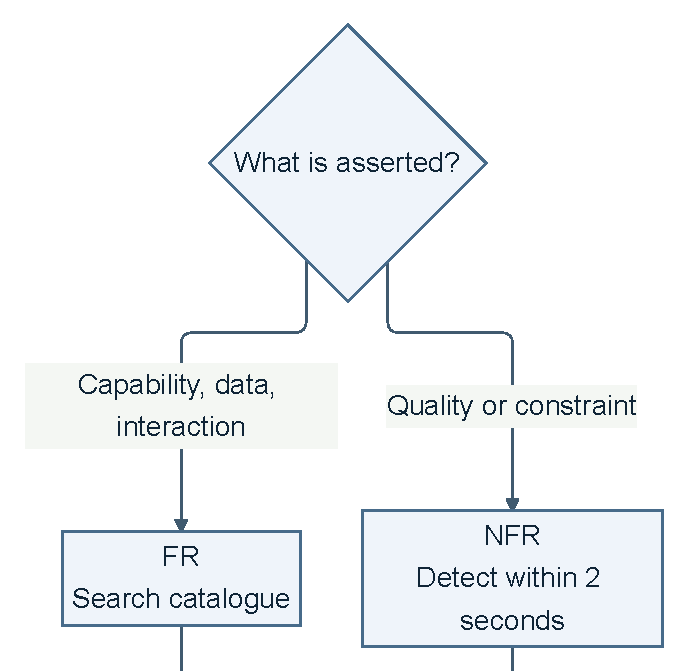
\includegraphics[width=202.86pt]{images/fig-003-compact-1.pdf}\end{minipage}\hfill
\begin{minipage}[t]{0.488\linewidth}\centering\scriptsize\textbf{2}\par\smallskip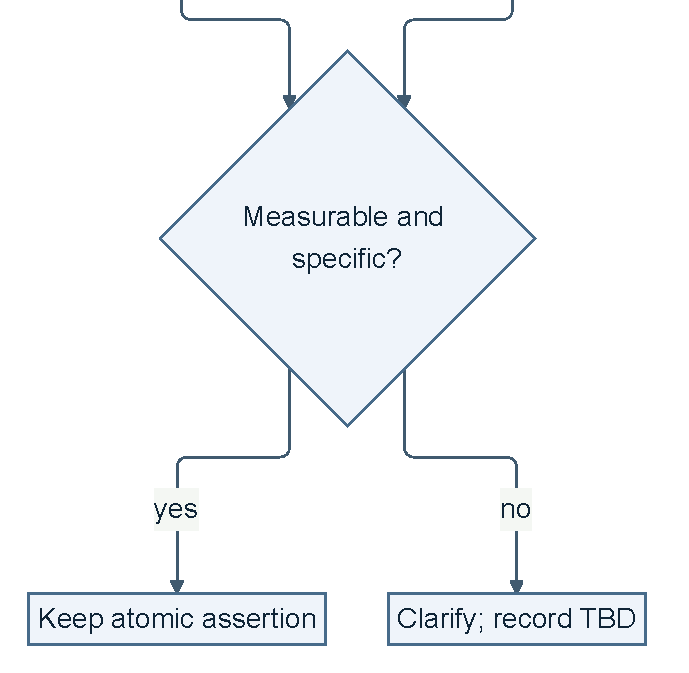
\includegraphics[width=202.86pt]{images/fig-003-compact-2.pdf}\end{minipage}
\captionof{figure}{classify a requirement --- follow numbered panels; crossing arrows continue.}\end{minipage}\par\smallskip

\begin{studycolumns}
\vspace{0pt}



\needspace{4\baselineskip}
\subsection*{2.1 Project mission statement}
\sectionlabel{h-21-project-mission-statement}
Two or three sentences that define:

\begin{enumerate}
\item \textbf{The problem} --- what will be done (scope and limits).
\item \textbf{The stakeholders} --- developers and users.
\item \textbf{The outcomes and benefits} --- plus a completion criterion.
\end{enumerate}


A mission statement may appear in the SRS product description (Writing SRS pp. 7--8).

\needspace{4\baselineskip}
\subsection*{2.2 Elicitation techniques (six --- memorise the list)}
\sectionlabel{h-22-elicitation-techniques-six--memorise-the-list}

\begin{referenceentries}
\textit{\textbf{Technique} / \textbf{Use when}}\par\smallskip
\noindent \textbf{\textbf{Interview}}: You need depth from one stakeholder; open questions\par
\noindent \textbf{\textbf{Observation}}: Users cannot articulate what they do ("watch the work")\par
\noindent \textbf{\textbf{Workshop}}: Many stakeholders must agree; resolve conflicts fast\par
\noindent \textbf{\textbf{Legacy product study}}: Replacing an existing system; inherit its quirks\par
\noindent \textbf{\textbf{Competitive product study}}: No access to users; derive features from rivals\par
\noindent \textbf{\textbf{Prototype}}: Requirements are visual/\allowbreak{}interaction-heavy; "a picture is worth a thousand words"\par
\end{referenceentries}
Two goals behind all six: \textbf{learn the problem domain} and \textbf{study user tasks}.

\textbf{Trap:} prototypes can elicit needs or validate them; state which purpose applies.
\end{studycolumns}

\Needspace{4\baselineskip}
\subsection*{2.3 Functional vs non-functional requirements}
\sectionlabel{h-23-functional-vs-non-functional-requirements}


{\fontsize{9}{11}\selectfont
\begin{longtable}{L{\dimexpr 0.17184\linewidth-4.12pt\relax}L{\dimexpr 0.40431\linewidth-9.70pt\relax}L{\dimexpr 0.42384\linewidth-10.17pt\relax}}
\toprule
\rowcolor{ice}\textbf{} & \textbf{\textbf{Functional}} & \textbf{\textbf{Non-functional}} \\
\midrule\endfirsthead
\toprule\rowcolor{ice}\textbf{} & \textbf{\textbf{Functional}} & \textbf{\textbf{Non-functional}} \\
\midrule\endhead
\multicolumn{3}{r}{\scriptsize Continued on next page}\\\endfoot
\bottomrule\endlastfoot
Definition & Interactions between the system and its environment; maps program inputs to program outputs & Properties the system must have, not directly related to functional behaviour \\
Answers & \emph{What must the system do?} & \emph{How well must it do it?} \\
Sub-kinds & System functionality \ensuremath{\cdot} Information to be processed \ensuremath{\cdot} Interface with other systems & Usability \ensuremath{\cdot} Reliability \ensuremath{\cdot} Performance \ensuremath{\cdot} Supportability (also security, availability, scalability, maintainability, portability) \\
Example & "The library member must be able to search the library catalog." & "When a book is placed on the checkout pad, the system must detect it within 2 seconds." \\
Example & "The system must display the temperature in degrees centigrade in the range \ensuremath{-}10 \textdegree{}C to +130 \textdegree{}C to one decimal place." & "Help messages must be displayed in the local language according to the user's locale." \\
Example & "The system must be able to control up to six robot arms simultaneously." & "After a system reboot, the full system functionality must be restored within 5 minutes." \\
\end{longtable}
}

\textbf{Classification drill (high-yield).} Decide which of these are FR vs NFR:




{\fontsize{9}{11}\selectfont
\begin{longtable}{L{\dimexpr 0.44456\linewidth-10.67pt\relax}L{\dimexpr 0.22664\linewidth-5.44pt\relax}L{\dimexpr 0.32880\linewidth-7.89pt\relax}}
\toprule
\rowcolor{ice}\textbf{Statement} & \textbf{Answer} & \textbf{Why} \\
\midrule\endfirsthead
\toprule\rowcolor{ice}\textbf{Statement} & \textbf{Answer} & \textbf{Why} \\
\midrule\endhead
\multicolumn{3}{r}{\scriptsize Continued on next page}\\\endfoot
\bottomrule\endlastfoot
The system must display the current time in 24-hour format & \textbf{FR} & Information to be processed \\
The database must be replaceable with any commercial product supporting standard SQL & \textbf{NFR} (supportability) & Portability/\allowbreak{}replaceability property \\
The system must verify membership with the University Account System before a loan & \textbf{FR} & Interface with another system \\
80\% of first-time users must enter a simple search query within 2 minutes & \textbf{NFR} (usability) & Measurable quality target \\
The system must log the event when the email server is unreachable & \textbf{FR} & Functionality (though see Section 3 --- may be an exception flow) \\
The system must be user-friendly & \textbf{NFR, but not verifiable as written} & Usability intent; needs a measurable criterion \\
\end{longtable}
}

\begin{studycolumns}
\vspace{0pt}


\begin{quote}\small\color{navy}
\textbf{Trap:} the "control up to six robot arms" example is \textbf{functional} (number of controllable devices is a capability), while "response within 2 seconds" is \textbf{performance/\allowbreak{}NFR}. Do not classify by the presence of a number --- classify by \textbf{what is being asserted}.

\end{quote}
\needspace{4\baselineskip}
\subsection*{2.4 Atomic, verifiable, traceable}
\sectionlabel{h-24-atomic-verifiable-traceable}
\textbf{Atomic} --- one testable assertion per numbered statement. Nest sub-requirements.


\begin{quote}\small\color{navy}
\emph{Original:} "When a computer is added, the tracking system requires the user to specify its type and allow the user to provide a description. Both these fields must be text of length > 0 and < 512."


\begin{ReferenceCode}
1.1   When a computer is added to the tracking system, the user must enter the computer type.
1.1.1 The computer type data must be text of at least one character and less than 512 characters.
1.2   When a computer is added to the tracking system, the user must enter a description.
1.2.1 The description of the computer must be text of at least one character and less than 512 characters.
\end{ReferenceCode}
\end{quote}
\textbf{Verifiable} --- sufficiently specific to be testable, with an oracle.


\begin{referenceentries}
\textit{\textbf{NO Not verifiable} / \textbf{YES Verifiable}}\par\smallskip
\noindent \textbf{NO Not verifiable:} The user interface must be user-friendly.\par
\noindent \textbf{YES Verifiable:} 80\% of first-time users must be able to enter a simple search query within 2 minutes of starting to use the system.\par\smallskip
\noindent \textbf{NO Not verifiable:} The system must control more than one drill press.\par
\noindent \textbf{YES Verifiable:} The system must control up to seven drill presses concurrently.\par\smallskip
\noindent \textbf{NO Not verifiable:} The company must not hire too-young or too-old people.\par
\noindent \textbf{YES Verifiable:} 0--15 and 55--99: do not hire; 16--17: part-time; 18--54: full-time.\par\smallskip
\end{referenceentries}
\textbf{Traceability} --- \emph{the ability to track requirements from their expression in the SRS to their realisation in design, documentation, source code, and their verification in reviews and tests; and to track dependencies among requirements, system functions and system components.}


\begin{quote}\small\color{navy}
\textbf{Trap:} traceability is \textbf{not} just "numbering requirements". Numbering is a prerequisite (modifiability); traceability is the \textbf{link} forwards (to design/\allowbreak{}code/\allowbreak{}test) and backwards (to source).

\end{quote}
\needspace{4\baselineskip}
\subsection*{2.5 Data dictionary (problem-domain glossary)}
\sectionlabel{h-25-data-dictionary-problem-domain-glossary}
The table below is the lecture's \textbf{illustrative university domain}, not a statement of NTU's academic calendar.

\begin{itemize}
\item Ensures \emph{consistent, unambiguous terminology} that all stakeholders agree on.
\item Defines \textbf{problem-domain} terms (Programme of Study, Course, Lecture, Tutorial, Class, Laboratory, Seminar) --- \textbf{not} implementation terms (table, foreign key, thread).
\end{itemize}

\begin{referenceentries}
\textit{\textbf{Term} / \textbf{Definition}}\par\smallskip
\noindent \textbf{Programme of Study}: A university programme a student enrols into. Three levels: undergraduate, master, PhD.\par
\noindent \textbf{Semester}: Four per academic year. Semesters 1 and 4 have 13 teaching weeks; semesters 2 and 3 have 5.\par
\noindent \textbf{Course}: A basic unit of teaching; compulsory or elective; must include lectures and tutorials; some have labs.\par
\noindent \textbf{Lecture}: Traditional class in lecture theatres; video recorded and published in the LMS.\par
\noindent \textbf{Tutorial}: Interactive, small-size class in technology-enhanced rooms; \textbf{not} video recorded.\par
\end{referenceentries}

\begin{quote}\small\color{navy}
\textbf{Trap:} the data dictionary is part of the SRS (Section 5 of the SRS contents). It is not a database schema and not a class diagram.

\end{quote}
\needspace{4\baselineskip}
\subsection*{2.6 Requirements validation}
\sectionlabel{h-26-requirements-validation}

\begin{referenceentries}
\textit{\textbf{Technique} / \textbf{What it checks}}\par\smallskip
\noindent \textbf{\textbf{Review} (walkthrough, inspection, critical review) with a checklist}: completeness, consistency, unambiguity, correctness\par
\noindent \textbf{\textbf{Prototype}}: Stakeholders: the system specified meets their needs/\allowbreak{}desires (\textbf{correct}) and requirements are \textbf{prioritised}. Development team: requirements and underlying assumptions are \textbf{properly understood}.\par
\end{referenceentries}

\begin{quote}\small\color{navy}
\textbf{Trap:} review \ensuremath{\neq} testing. Review is \textbf{static} (document inspection); testing is \textbf{dynamic} (execution). Both appear as "validation" in different lectures --- read the context.

\end{quote}
\needspace{4\baselineskip}
\subsection*{2.7 The iterative elicitation loop (memorise the steps)}
\sectionlabel{h-27-the-iterative-elicitation-loop-memorise-the-steps}
\textbf{Step 1 --- Project team alone.} Review the client's specification (and legacy/\allowbreak{}competitive products) to:

\begin{enumerate}
\item \textbf{Atomise} requirements.
\item Identify \textbf{actors}.
\item Identify main \textbf{use cases} (functional requirements).
\item Identify \textbf{non-functional} requirements.
\item Initiate the \textbf{data dictionary}.
\item Identify \textbf{uncertainties \ensuremath{\rightarrow} TBD} (To Be Determined). \emph{Never guess user requirements.}
\end{enumerate}
\textbf{Step 2 --- Project team meets client} (interview /\allowbreak{} observation /\allowbreak{} workshop). Agenda agreed up-front:

\begin{enumerate}
\item Present and walk through the initial requirements + data dictionary \ensuremath{\rightarrow} get agreement.
\item Clarify the TBD issues.
\item Discuss new requirements the client raises.
\end{enumerate}
Repeat 1--2 \textbf{until} all uncertainties and ambiguities in functional, non-functional requirements and data-dictionary terms are agreed with the client. A prototype may be produced to show intended functionality. \textbf{Minimise the number of meetings by making meetings productive.}


\begin{quote}\small\color{navy}
\textbf{Trap:} "Do not guess the user requirements" is an explicit lecture instruction --- the correct answer to a missing requirement is \textbf{TBD + ask the client}, not "assume a sensible default".

\end{quote}
\end{studycolumns}

\chapteropen{Chapter 3: Use-case modelling}{chapter-3}
\markboth{Ch. 3 | Use cases}{}


\begin{studycolumns}
\vspace{0pt}
\begin{eli5box}
A use case is a promise about a user's goal, like 'borrow a book'. An actor is a role standing outside the system. The diagram is the menu of goals; the description is the recipe showing what the user and system do, including what happens when something goes wrong.
\end{eli5box}
\textbf{Answer check:} Start with the boundary and external roles; name goals, then describe actor/system steps and alternatives. Include is required reuse; extend is conditional extra behaviour. Neither means ``happens next. Authentication may be a precondition without a fresh login each time. Keep denial/conflict paths inside the behaviour when they must be explained.
\needspace{4\baselineskip}
\subsection*{Visual: decide between include and extend}
\sectionlabel{h-visual-decide-between-include-and-extend}
First identify a meaningful unit of behaviour; do not turn every sentence into a use case.
\end{studycolumns}


\par\smallskip\noindent\begin{minipage}{\linewidth}\centering
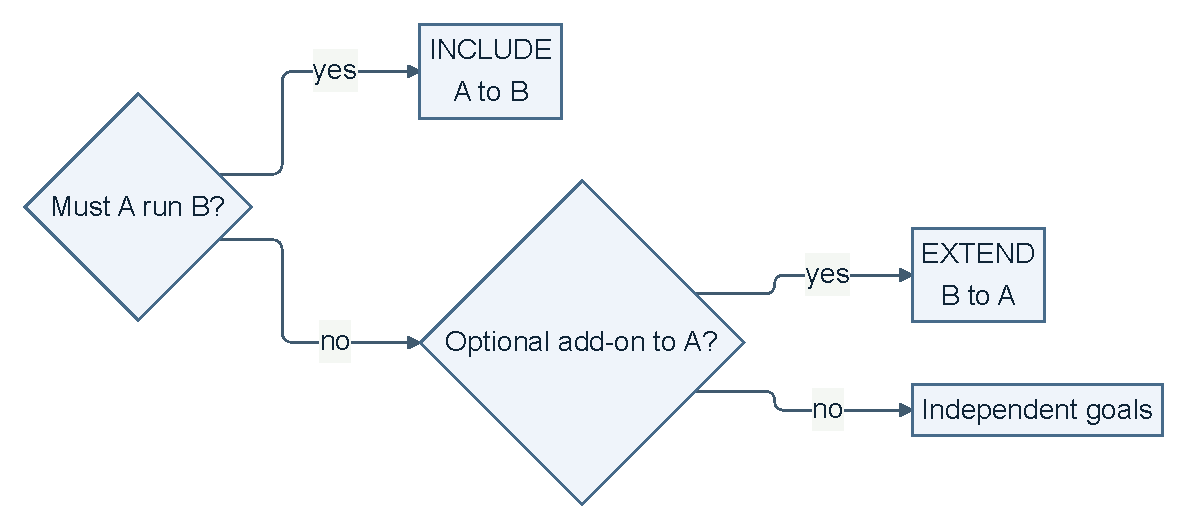
\includegraphics[width=349.60pt]{images/fig-004.pdf}
\captionof{figure}{decide between include and extend}\end{minipage}\par\smallskip

\begin{studycolumns}
\vspace{0pt}



\needspace{4\baselineskip}
\subsection*{3.1 UML in one table}
\sectionlabel{h-31-uml-in-one-table}
UML = \emph{a graphical notation with textual annotation for specifying, documenting and communicating structure, functionality and dynamic behaviour of complex software systems.} Booch + Jacobson + Rumbaugh; the lecture gives UML 1.1 adoption in 1997 and refers to UML 2.5 (2015). These are historical references in the supplied slides, not a claim about the current UML release.


\begin{referenceentries}
\textit{\textbf{Category} / \textbf{Diagrams}}\par\smallskip
\noindent \textbf{\textbf{Structure} (static, "irrespective of time")}: Class, Object, Package, Component, Composite Structure, Deployment (L3 list)\par
\noindent \textbf{\textbf{Behaviour} (dynamic)}: \textbf{Use Case}, \textbf{Activity}, \textbf{State Machine}, \textbf{Sequence}, \textbf{Communication}, Interaction Overview, Timing\par
\end{referenceentries}
Course modelling focus: \textbf{use case, class, sequence, state machine, activity} (communication/\allowbreak{}object appear in the SRS figure list).

\textbf{Trap:} UML is \textbf{not} a programming language and \textbf{not} a method. "Only use the diagrams that are useful and necessary to define the system" --- select diagrams for the modelling need rather than drawing every diagram type.

\needspace{4\baselineskip}
\subsection*{3.2 Use case model = static + dynamic}
\sectionlabel{h-32-use-case-model--static--dynamic}

\begin{quote}\small\color{navy}
\textbf{Use case model = Use case diagram (static) + Use case descriptions (dynamic).}

\end{quote}
The diagram identifies relationships; the description specifies the behaviour. Supply both when requested.
\end{studycolumns}

\Needspace{4\baselineskip}
\subsection*{3.3 Diagram elements}
\sectionlabel{h-33-diagram-elements}


{\fontsize{9}{11}\selectfont
\begin{longtable}{L{\dimexpr 0.22801\linewidth-5.47pt\relax}L{\dimexpr 0.36291\linewidth-8.71pt\relax}L{\dimexpr 0.40908\linewidth-9.82pt\relax}}
\toprule
\rowcolor{ice}\textbf{Element} & \textbf{Notation} & \textbf{Meaning} \\
\midrule\endfirsthead
\toprule\rowcolor{ice}\textbf{Element} & \textbf{Notation} & \textbf{Meaning} \\
\midrule\endhead
\multicolumn{3}{r}{\scriptsize Continued on next page}\\\endfoot
\bottomrule\endlastfoot
\textbf{Actor} & Stick figure, labelled with role (not a person's name) & An \textbf{external} entity that interacts with the system \\
\textbf{Use case} & Ellipse, labelled with a verb phrase & A unit of functionality performed by the system yielding a result/\allowbreak{}value for an actor \\
\textbf{Association} & Solid line actor\ensuremath{\leftrightarrow}use case & Actor participates in that use case \\
\textbf{System boundary} & Rectangle around use cases & Separates system from environment \\
\textbf{Generalization} & Solid line, hollow triangle pointing to the parent & Actor or use-case specialisation \\
\textbf{\guillemotleft{}include\guillemotright{}} & Dashed arrow from base \ensuremath{\rightarrow} included & Base \textbf{always} performs the included behaviour \\
\textbf{\guillemotleft{}extend\guillemotright{}} & Dashed arrow from extending \ensuremath{\rightarrow} base & Extending behaviour is \textbf{optional/\allowbreak{}conditional} \\
\end{longtable}
}


\Needspace{4\baselineskip}
\subsection*{3.4 \guillemotleft{}include\guillemotright{} vs \guillemotleft{}extend\guillemotright{} --- decomposition, reuse and optional behaviour}
\sectionlabel{h-34-include-vs-extend--decomposition-reuse-and-optional-behaviour}


{\fontsize{9}{11}\selectfont
\begin{longtable}{L{\dimexpr 0.22236\linewidth-5.34pt\relax}L{\dimexpr 0.43297\linewidth-10.39pt\relax}L{\dimexpr 0.34467\linewidth-8.27pt\relax}}
\toprule
\rowcolor{ice}\textbf{} & \textbf{\textbf{\guillemotleft{}include\guillemotright{}}} & \textbf{\textbf{\guillemotleft{}extend\guillemotright{}}} \\
\midrule\endfirsthead
\toprule\rowcolor{ice}\textbf{} & \textbf{\textbf{\guillemotleft{}include\guillemotright{}}} & \textbf{\textbf{\guillemotleft{}extend\guillemotright{}}} \\
\midrule\endhead
\multicolumn{3}{r}{\scriptsize Continued on next page}\\\endfoot
\bottomrule\endlastfoot
Trigger & Always, as part of the base & Under an explicit condition /\allowbreak{} at an extension point \\
Purpose & Functional decomposition, or \textbf{reuse} of common behaviour & Add \textbf{optional} functionality \\
Base alone is\ldots{} & \textbf{Incomplete} without the included UC & \textbf{Complete by itself} \\
Arrow direction & base ----\ensuremath{\blacktriangleright} included & extending ----\ensuremath{\blacktriangleright} base \\
Course example & Manage Incident \textbf{includes} Create /\allowbreak{} Handle /\allowbreak{} Close Incident; Open Incident and Allocate Resources \textbf{include} View Map & Report Emergency \ensuremath{\blacktriangleleft}---- \textbf{extends} ---- Help \\
\end{longtable}
}

\begin{studycolumns}
\vspace{0pt}


\begin{quote}\small\color{navy}
\textbf{Trap \#1 (arrow direction).} Students reverse \guillemotleft{}extend\guillemotright{} arrows constantly. Mnemonic: \textbf{"include points to the helper; extend points to the host."}

\textbf{Trap:} conditional behaviour can remain an alternative/exception flow. Use extend only for a separate optional unit; required reused behaviour uses include.


\end{quote}
\needspace{4\baselineskip}
\subsection*{3.5 The use case description --- mandatory fields}
\sectionlabel{h-35-the-use-case-description--mandatory-fields}
\begin{enumerate}
\item \textbf{Participating actors} (with the \textbf{initiating actor} identified).
\begin{itemize}
\item A use case can have more than one participating actor.
\item The \textbf{initiating actor triggers} the use case.
\item If triggered by a \textbf{system event or another use case}, the initiating actor is \textbf{NULL}.
\end{itemize}
\item \textbf{Entry conditions (pre-condition)} --- system state that must be satisfied to execute.
\item \textbf{Exit conditions (post-condition)} --- system state that must be reached afterwards.
\item \textbf{Flow of events} (a.k.a. normal /\allowbreak{} main success flow) --- alternating actor and system steps: step 1 = how the actor triggers; step 2 = how the system responds; \ldots{}
\item \textbf{Alternative flows} --- variations or errors that \textbf{return to the normal flow} (e.g. invalid card/\allowbreak{}PIN \ensuremath{\rightarrow} back to step 2; insufficient funds \ensuremath{\rightarrow} back to step 6).
\item \textbf{Exceptions} --- exceptional situations that \textbf{cause the use case to fail} (e.g. three invalid PIN attempts \ensuremath{\rightarrow} card suspended; ATM out of funds \ensuremath{\rightarrow} refuses card).
\end{enumerate}
Template also captures: Use Case ID, Name, Created/\allowbreak{}Updated by, dates, Actor, Description, Priority, Frequency of Use, Includes, Special Requirements, Assumptions, Notes and Issues.

\needspace{4\baselineskip}
\subsection*{3.6 Worked example --- "Withdraw Money using ATM"}
\sectionlabel{h-36-worked-example--withdraw-money-using-atm}
\textbf{Participating actors:} Bank Customer (\textbf{initiating}), Bank (secondary/\allowbreak{}external system). \textbf{Entry conditions:} (1) customer has an account with the bank \textbf{and} (2) has an ATM card and PIN. \textbf{Exit conditions:} (1) customer receives the requested cash \textbf{or} (2) customer receives an explanation from the ATM why cash could not be dispensed.

\textbf{Normal flow (note the A/\allowbreak{}S alternation):}
\end{studycolumns}


{\fontsize{9}{11}\selectfont
\begin{longtable}{L{\dimexpr 0.14850\linewidth-3.56pt\relax}L{\dimexpr 0.35357\linewidth-8.49pt\relax}L{\dimexpr 0.49793\linewidth-11.95pt\relax}}
\toprule
\rowcolor{ice}\textbf{\#} & \textbf{Actor step} & \textbf{System step} \\
\midrule\endfirsthead
\toprule\rowcolor{ice}\textbf{\#} & \textbf{Actor step} & \textbf{System step} \\
\midrule\endhead
\multicolumn{3}{r}{\scriptsize Continued on next page}\\\endfoot
\bottomrule\endlastfoot
1 & Inputs the card into the ATM &  \\
2 &  & Requests input of a six-digit PIN \\
3 & Enters a PIN &  \\
4 &  & Verifies card and PIN with account info in the Bank \\
5 &  & If verified, requests the amount to withdraw \\
6 & Enters an amount &  \\
7 &  & Verifies the amount is available in the account \\
8 &  & If sufficient funds, outputs money, card and receipt \\
9 & Removes card, receipt and money &  \\
\end{longtable}
}

\begin{studycolumns}
\vspace{0pt}

\textbf{Alternative flows}

\begin{itemize}
\item \textbf{AF-S5 (invalid card and PIN):} 1. ATM displays "Invalid card and PIN. Please try again!" for 2 s. 2. ATM \textbf{returns to step 2}.
\item \textbf{AF-S8 (insufficient funds):} 1. ATM displays "Insufficient funds\ldots{} enter a smaller amount!" for 2 s. 2. ATM \textbf{returns to step 6}.
\end{itemize}
\textbf{Exceptions}

\begin{itemize}
\item \textbf{EX1 (invalid PIN three times):} 1. Displays "Card is suspended! Please call customer service (1633)\ldots{}" for 2 s. 2. Outputs the card. \ensuremath{\rightarrow} \emph{Use case fails.}
\item \textbf{EX2 (ATM has insufficient funds):} 1. Displays "This ATM is off-service due to insufficient funds!" at the start screen. 2. Does not accept the card.
\end{itemize}

\begin{quote}\small\color{navy}
\textbf{Trap:} the AF/\allowbreak{}EX distinction is graded. \textbf{AF = recoverable, returns to a step. EX = terminal, the goal is not achieved.} "Insufficient funds in \emph{account}" is recoverable (AF); "insufficient funds in \emph{ATM}" is not (EX). Read carefully which one the question describes.

\end{quote}
\needspace{4\baselineskip}
\subsection*{3.7 Deriving use cases from functional requirements}
\sectionlabel{h-37-deriving-use-cases-from-functional-requirements}
Use the Library Management System drill (L3):
\end{studycolumns}


{\fontsize{9}{11}\selectfont
\begin{longtable}{L{\dimexpr 0.07599\linewidth-3.04pt\relax}L{\dimexpr 0.33209\linewidth-13.28pt\relax}L{\dimexpr 0.21261\linewidth-8.50pt\relax}L{\dimexpr 0.19839\linewidth-7.94pt\relax}L{\dimexpr 0.18092\linewidth-7.24pt\relax}}
\toprule
\rowcolor{ice}\textbf{\#} & \textbf{Functional requirement} & \textbf{Actor(s)} & \textbf{Use case} & \textbf{Association} \\
\midrule\endfirsthead
\toprule\rowcolor{ice}\textbf{\#} & \textbf{Functional requirement} & \textbf{Actor(s)} & \textbf{Use case} & \textbf{Association} \\
\midrule\endhead
\multicolumn{5}{r}{\scriptsize Continued on next page}\\\endfoot
\bottomrule\endlastfoot
1 & Member searches for materials & Member & Search Material & --- \\
2 & Member loans materials & Member & Loan Material & --- \\
3 & System verifies membership with University Account System \textbf{before} loan & Member, University Account System & Verify Member & \guillemotleft{}include\guillemotright{} from Loan Material \\
4 & Member returns materials via drop-off kiosk & Member, Library Drop-off Kiosk & Return Material & --- \\
5 & System sends overdue notice via CITS Email Server & CITS Email System & Send Overdue Notice & --- \\
6 & \textbf{When} network to CITS fails, log the event & --- (system event) & Log Network Issues & \guillemotleft{}extend\guillemotright{} on Send Overdue Notice \\
\end{longtable}
}

\begin{studycolumns}
\vspace{0pt}

\textbf{Method (do this in the exam, in order):}

\begin{enumerate}
\item \textbf{Identify actors} --- scan for \emph{people/\allowbreak{}roles} and \emph{external systems}; underline nouns.
\item \textbf{Identify use cases} --- scan for \emph{verb phrases describing a goal} ("search", "loan", "return", "send notice"). One goal = one use case.
\item \textbf{Identify associations} --- draw actor\ensuremath{\leftrightarrow}UC lines only where the actor participates.
\item \textbf{Add include/\allowbreak{}extend/\allowbreak{}generalization} --- only where justified; annotate with one sentence of reasoning.
\item \textbf{Write the description} for the use cases the question names.
\end{enumerate}
\textbf{Lecture comparison.} L3, pp. 20--22, shows three candidate library diagrams, including different choices of actor and authentication behaviour. Do not treat every candidate as an approved solution. Trace each element to the stated requirements: membership verification is required before a loan; Login is not stated for the library example. L4, pp. 12--16, separately uses Login in the course registration example. Explain the system boundary and reuse choice.

\textbf{Trap --- actors vs system internals.} "Database", "Sensor" (if part of the system's own hardware), "UI" are \textbf{not} actors. But an \textbf{external} University Account System, CITS Email Server, Billing System, Library Drop-off Kiosk \textbf{are} actors.

\textbf{Trap --- actor generalization.} If Student and Professor share Login, model an abstract \textbf{User} actor with generalization arrows from Student/\allowbreak{}Professor to User, then associate Login with User. Do not draw duplicate Logins.
\end{studycolumns}

\chapteropen{Chapter 4: Conceptual models and class diagrams}{chapter-4}
\markboth{Ch. 4 | Class diagrams}{}


\begin{studycolumns}
\vspace{0pt}
\begin{eli5box}
Think of a cinema: a TicketScreen talks to the customer, a BookingController organises the booking and a Ticket stores a booking fact. A class is a kind of thing; an object is one particular instance. A link's numbers tell you how many objects can be connected, not which class owns the drawing.
\end{eli5box}
\textbf{Answer check:} Separate boundaries, coordinating controls and persistent entities. Conceptual questions may prohibit attributes/operations; add them only for detailed design. State invariants that multiplicities cannot express, such as one active hold despite many historical holds.
\end{studycolumns}

\subsection*{Visual: assign each class a responsibility}
\sectionlabel{h-visual-assign-each-class-a-responsibility}


\par\smallskip\noindent\begin{minipage}{\linewidth}\centering
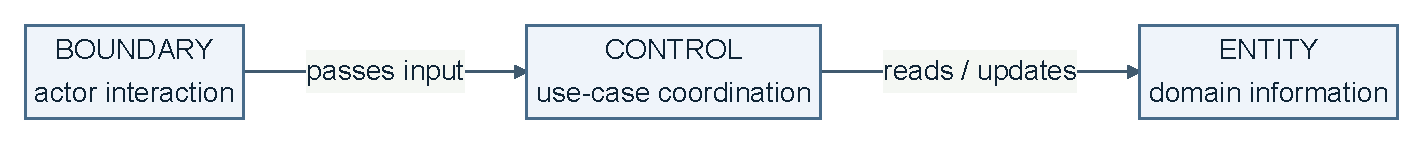
\includegraphics[width=419.06pt]{images/fig-005.pdf}
\captionof{figure}{assign each class a responsibility}\end{minipage}\par\smallskip



The boundary/control/entity arrows show a common collaboration, not every allowed relationship; derive responsibilities from the case.


\Needspace{4\baselineskip}
\subsection*{4.1 Elicitation vs analysis (L5 distinction)}
\sectionlabel{h-41-elicitation-vs-analysis-l5-distinction}


{\fontsize{9}{11}\selectfont
\begin{longtable}{L{\dimexpr 0.19613\linewidth-4.71pt\relax}L{\dimexpr 0.35448\linewidth-8.51pt\relax}L{\dimexpr 0.44939\linewidth-10.79pt\relax}}
\toprule
\rowcolor{ice}\textbf{} & \textbf{\textbf{Requirements elicitation}} & \textbf{\textbf{Requirements analysis}} \\
\midrule\endfirsthead
\toprule\rowcolor{ice}\textbf{} & \textbf{\textbf{Requirements elicitation}} & \textbf{\textbf{Requirements analysis}} \\
\midrule\endhead
\multicolumn{3}{r}{\scriptsize Continued on next page}\\\endfoot
\bottomrule\endlastfoot
Purpose & Find out \textbf{what customers want} & Produce a system model that is \textbf{correct, complete, consistent, unambiguous} based on the use cases \\
Output & Description of the system in terms of \textbf{actors and use cases} & \textbf{Conceptual model} (system structure) + \textbf{dynamic model} (system behaviour) \\
Perspective & Customer's & Software engineer's \\
Artefacts & SRS, use case diagram + descriptions, data dictionary, prototype & Class diagram (boundary/\allowbreak{}control/\allowbreak{}entity), sequence diagrams, state machines, activity diagrams \\
\end{longtable}
}

Formalising requirements with analysis models: \textbf{clarifies} structure and dynamics, \textbf{validates} requirements, \textbf{underpins} solution modelling.


\Needspace{4\baselineskip}
\subsection*{4.2 Conceptual model vocabulary}
\sectionlabel{h-42-conceptual-model-vocabulary}


{\fontsize{9}{11}\selectfont
\begin{longtable}{L{\dimexpr 0.21676\linewidth-5.20pt\relax}L{\dimexpr 0.37413\linewidth-8.98pt\relax}L{\dimexpr 0.40912\linewidth-9.82pt\relax}}
\toprule
\rowcolor{ice}\textbf{Element} & \textbf{Definition} & \textbf{Example} \\
\midrule\endfirsthead
\toprule\rowcolor{ice}\textbf{Element} & \textbf{Definition} & \textbf{Example} \\
\midrule\endhead
\multicolumn{3}{r}{\scriptsize Continued on next page}\\\endfoot
\bottomrule\endlastfoot
\textbf{Object} & Anything that has a \textbf{state} and exhibits \textbf{behaviour} & Bus, Dog, Company; \emph{LoginForm, UserVerifier, UserList} \\
\textbf{Operation} & Procedure through which objects communicate & Bus: Stop, Start; Company: Sell, Quote; UserVerifier: authenticate \\
\textbf{Attribute} & Variable holding state information & Bus: Seats, Colour; Company: Name, Employees \\
\end{longtable}
}

\begin{studycolumns}
\vspace{0pt}

Documented in a \textbf{class diagram}: Object \ensuremath{\rightarrow} Class; Roles of the object \ensuremath{\rightarrow} Attributes and methods of the class.


\needspace{152pt}
\subsection*{4.3 Class notation}
\sectionlabel{h-43-class-notation}

\par\smallskip\noindent\begin{minipage}{\linewidth}\centering
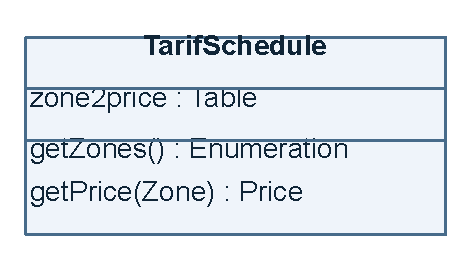
\includegraphics[width=138.46pt]{images/fig-006.pdf}
\captionof{figure}{4.3 Class notation}\end{minipage}\par\smallskip


\end{studycolumns}
\Needspace{110pt}
\subsection*{4.4 Relationships --- notation and reading}
\sectionlabel{h-44-relationships--notation-and-reading}

\needspace{4\baselineskip}
\subsubsection*{What the relationships look like}
\sectionlabel{h-what-the-relationships-look-like}
The following are concrete class-diagram sketches. Read the symbol \textbf{at the end of the line} carefully: that is where the relationship is attached.


\begin{center}
\begin{minipage}[t]{.235\linewidth}\centering\small\textbf{Association: structural link; navigation unspecified}\par\smallskip

\includegraphics[width=.88\linewidth,height=75pt,keepaspectratio]{images/fig-007.pdf}\end{minipage}
\hfill
\begin{minipage}[t]{.235\linewidth}\centering\small\textbf{Navigability: reach the arrow-end class}\par\smallskip

\includegraphics[width=.88\linewidth,height=75pt,keepaspectratio]{images/fig-008.pdf}\end{minipage}
\hfill
\begin{minipage}[t]{.235\linewidth}\centering\small\textbf{Non-navigable: Person cannot reach Course}\par\smallskip

\includegraphics[width=.88\linewidth,height=75pt,keepaspectratio]{images/fig-009.pdf}\end{minipage}
\hfill
\begin{minipage}[t]{.235\linewidth}\centering\small\textbf{Generalization: triangle at parent; no multiplicity}\par\smallskip
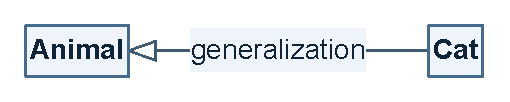
\includegraphics[width=.88\linewidth,height=75pt,keepaspectratio]{images/fig-010.pdf}\end{minipage}
\par\medskip
\begin{minipage}[t]{.235\linewidth}\centering\small\textbf{Abstract superclass: cannot instantiate}\par\smallskip
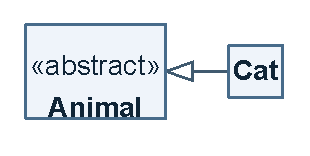
\includegraphics[width=.88\linewidth,height=75pt,keepaspectratio]{images/fig-011.pdf}\end{minipage}
\hfill
\begin{minipage}[t]{.235\linewidth}\centering\small\textbf{Realization: implements an interface}\par\smallskip
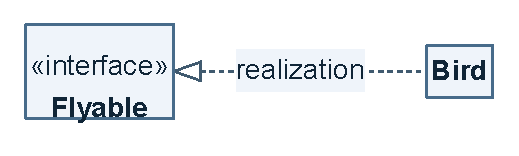
\includegraphics[width=.88\linewidth,height=75pt,keepaspectratio]{images/fig-012.pdf}\end{minipage}
\hfill
\begin{minipage}[t]{.235\linewidth}\centering\small\textbf{Aggregation: parts can outlive the whole}\par\smallskip

\includegraphics[width=.88\linewidth,height=75pt,keepaspectratio]{images/fig-013.pdf}\end{minipage}
\hfill
\begin{minipage}[t]{.235\linewidth}\centering\small\textbf{Composition: exclusive ownership and lifecycle}\par\smallskip

\includegraphics[width=.88\linewidth,height=75pt,keepaspectratio]{images/fig-014.pdf}\end{minipage}
\par\medskip
\begin{minipage}[t]{.235\linewidth}\centering\small\textbf{Dependency: temporary use}\par\smallskip

\includegraphics[width=.88\linewidth,height=75pt,keepaspectratio]{images/fig-015.pdf}\end{minipage}
\hfill
\begin{minipage}[t]{.235\linewidth}\centering\small\textbf{Multiplicity: near-end class is counted}\par\smallskip
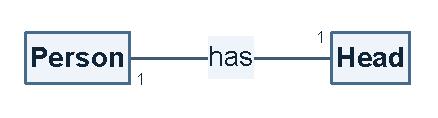
\includegraphics[width=.88\linewidth,height=75pt,keepaspectratio]{images/fig-016.pdf}\end{minipage}
\par\medskip
\par\smallskip\small Mermaid cannot draw UML's non-navigable x; place it at the Course end in an examination drawing.\par
\captionof{figure}{Relationship notation atlas: read the symbol at each end.}
\end{center}
\begin{studycolumns}
\textbf{Multiplicity cheatsheet}


\begin{referenceentries}
\textit{\textbf{Notation} / \textbf{Meaning}}\par\smallskip
\noindent \textbf{\code{1}}: Exactly one\par
\noindent \textbf{\code{0.\allowbreak{}.\allowbreak{}1}}: Zero or one (optional)\par
\noindent \textbf{\code{*} or \code{0.\allowbreak{}.\allowbreak{}*}}: Zero or more\par
\noindent \textbf{\code{1.\allowbreak{}.\allowbreak{}*}}: One or more\par
\noindent \textbf{\code{3}}: Exactly three\par
\noindent \textbf{\code{1.\allowbreak{}.\allowbreak{}6}}: Between one and six\par
\end{referenceentries}
\textbf{How to read a multiplicity correctly:} the number is written \textbf{at the end near the class it counts}. \code{Person "1" -\allowbreak{}-\allowbreak{} "1" Head} means one Head per Person and one Person per Head. \code{Polygon "1" -\allowbreak{}-\allowbreak{} "*" Point} means zero or more Points per Polygon and one Polygon per Point.

\textbf{Notation:} abstract class names are italicised or marked \code{\{abstract\}}; interface realisation uses a dashed line and hollow triangle.

\par\smallskip{\color{amber}\bfseries Traps and things to check}\par
Choose one relationship type per line. Generalization has a hollow triangle at the parent, no multiplicities or role names. Association multiplicities belong at both counted ends. A plain line leaves navigability unspecified; an x prohibits reaching its target end. Composition adds exclusive composite ownership and lifecycle responsibility; a part may be detached before deletion. Use hollow-triangle generalization despite L5's inconsistent filled-arrow example.
\par\smallskip
\end{studycolumns}

\Needspace{4\baselineskip}
\subsection*{4.5 Stereotypes: entity /\allowbreak{} boundary /\allowbreak{} control}
\sectionlabel{h-45-stereotypes-entity--boundary--control}


{\fontsize{9}{11}\selectfont
\begin{longtable}{L{\dimexpr 0.22883\linewidth-5.49pt\relax}L{\dimexpr 0.36549\linewidth-8.77pt\relax}L{\dimexpr 0.40568\linewidth-9.74pt\relax}}
\toprule
\rowcolor{ice}\textbf{Stereotype} & \textbf{Role} & \textbf{Typical examples} \\
\midrule\endfirsthead
\toprule\rowcolor{ice}\textbf{Stereotype} & \textbf{Role} & \textbf{Typical examples} \\
\midrule\endhead
\multicolumn{3}{r}{\scriptsize Continued on next page}\\\endfoot
\bottomrule\endlastfoot
\textbf{\guillemotleft{}entity\guillemotright{}} & Information tracked by the system & \code{Account}, \code{Silo}, \code{Shipment} \\
\textbf{\guillemotleft{}boundary\guillemotright{}} & Interaction between an actor and the system & \code{Login\allowbreak{}Form}, \code{Entry\allowbreak{}Gate}, \code{Fingerprint\allowbreak{}Reader} \\
\textbf{\guillemotleft{}control\guillemotright{}} & Logic that realises a use case (coordination) & \code{Facility\allowbreak{}Access\allowbreak{}System}, \code{Sheet\allowbreak{}Manager}, \code{Registration\allowbreak{}Controller} \\
\end{longtable}
}

\begin{studycolumns}
\vspace{0pt}

Worked example --- \textbf{EnterSecureFacility}:


\begin{quote}\small\color{navy}
\begin{enumerate}
\item User presses finger on FingerprintReader. 2. FingerprintReader scans and sends image to FacilityAccessSystem. 3. FacilityAccessSystem validates fingerprint and unlocks EntryGate.
\item EntryGate signals the system it has opened. 5. FacilityAccessSystem locks EntryGate, logs the entry event and increments occupant count.
\end{enumerate}
\end{quote}
Classes: \code{Employee} (\guillemotleft{}entity\guillemotright{}), \code{Fingerprint} (\guillemotleft{}entity\guillemotright{}), \code{Fingerprint\allowbreak{}Reader} (\guillemotleft{}boundary\guillemotright{}), \code{Entry\allowbreak{}Gate} (\guillemotleft{}boundary\guillemotright{}), \code{Facility\allowbreak{}Access\allowbreak{}System} (\guillemotleft{}control\guillemotright{}). Relations with stereotypes: \code{<<read>\allowbreak{}>\allowbreak{}}, \code{<<call>\allowbreak{}>\allowbreak{}}, \code{<<signal>\allowbreak{}>\allowbreak{}} (usage dependencies between them).


\needspace{4\baselineskip}
\subsection*{4.6 Four-step analysis procedure}
\sectionlabel{h-46-four-step-analysis-procedure}
\begin{enumerate}
\item Identify the \textbf{classes}.
\item Find the \textbf{attributes} for each class.
\item Find the \textbf{methods/\allowbreak{}operations} for each class.
\item Find the \textbf{associations} between classes.
\end{enumerate}
How to find classes:

\begin{enumerate}
\item \textbf{Recurring nouns/\allowbreak{}concepts} in the use cases.
\item \textbf{Real-world entities} the system must track.
\item \textbf{Application/\allowbreak{}problem-domain terms} in the data dictionary. Then \textbf{review definitions and attributes with stakeholders}.
\end{enumerate}

\begin{quote}\small\color{navy}
\textbf{Trap:} do \textbf{not} promote every noun to a class. If a noun has no attributes, no identity and no behaviour of its own (e.g. "amount", "date", "grade"), it is an \textbf{attribute}, not a class. Conversely "grade" in GES has an enumerated domain and constrains storage rules \ensuremath{\rightarrow} it can justify a class/\allowbreak{}type in the design model.

\end{quote}
\end{studycolumns}

\chapteropen{Chapter 5: State machines and activity diagrams}{chapter-5}
\markboth{Ch. 5 | Dynamic models}{}


\begin{studycolumns}
\vspace{0pt}
\begin{eli5box}
A traffic light has states such as Red and Green; 'change colour' is an action. A pizza-order workflow has activities such as take order, bake and deliver. Use a state machine to explain one object's changing condition; use an activity diagram to explain how work moves among participants.
\end{eli5box}
\textbf{Answer check:} Model the named object/workflow. Check guards, equality, cancellation, timeouts, retry counts and late replies. A dialog map models interaction/screens. Do not force a final node onto permanent monitoring; do not rename actions as states.
\end{studycolumns}

\subsection*{Visual: choose the diagram that answers the question}
\sectionlabel{h-visual-choose-the-diagram-that-answers-the-question}


\par\smallskip\noindent\begin{minipage}{\linewidth}\centering
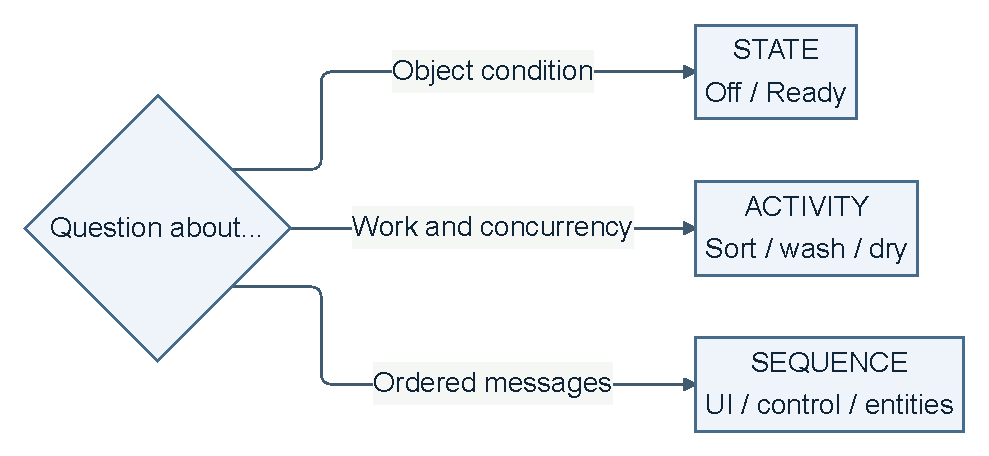
\includegraphics[width=291.18pt]{images/fig-017.pdf}
\captionof{figure}{choose the diagram that answers the question}\end{minipage}\par\smallskip

\begin{studycolumns}
\vspace{0pt}



\needspace{4\baselineskip}
\subsection*{5.1 State machine diagram (a.k.a. statechart, finite state automaton, \textbf{dialog map})}
\sectionlabel{h-51-state-machine-diagram-aka-statechart-finite-state-automaton-dialog-map}
\begin{itemize}
\item Models a system/\allowbreak{}object by the \textbf{states} it can be in.
\item \textbf{State} = a \emph{stable condition} that exists for a period (or all) of time until an \textbf{action/\allowbreak{}event} drives it to another stable state.
\item Finite number of states; transitions determined by previous state and actions.
\item Notation: rounded rectangle, name at top, optional \textbf{entry /\allowbreak{} action}, \textbf{exit /\allowbreak{} action}, \textbf{do /\allowbreak{} activity}.
\item A diagram begins with a \textbf{start node} (filled circle) and ends with an \textbf{end node} --- \textbf{unless} the system loops forever, in which case there is no end node.
\item A transition is \textbf{assumed instantaneous} in response to an event. Full label:
\end{itemize}

\begin{ReferenceCode}
event(arguments) [guard] / action
\end{ReferenceCode}
\textbf{Dialog map} = a state machine used to prototype navigation. Since most UIs show one screen/\allowbreak{}window at a time (a state) with defined conditions to move (transitions), dialog maps:

\begin{itemize}
\item find \textbf{missing or incorrect navigation pathways early}, when they are cheap to fix;
\item spot \textbf{reuse opportunities and redundancies} without premature screen design.
\end{itemize}
\textbf{Worked states:} see the case-specific dialog/state answers in the past papers. A self-transition exits and re-enters its state, so entry actions run again.

\textbf{Action semantics:} do may complete before state exit; entry/exit run on every entry/exit, including re-entry. Decision guards must be mutually exclusive and cover intended cases (or use \code{[else]}).

\needspace{4\baselineskip}
\subsection*{5.2 Activity diagram}
\sectionlabel{h-52-activity-diagram}
\begin{itemize}
\item \textbf{Activity} = execution of one or more basic operations (rounded rectangle).
\item \textbf{Control flow} = arrows.
\item \textbf{Fork} = one input, two or more \textbf{concurrent} outputs (\textbf{thick bar}).
\item \textbf{Join} = two or more flows come together into one (\textbf{thick bar}).
\item \textbf{Decision/\allowbreak{}branch} = one input, several guarded outputs (\textbf{diamond}).
\item \textbf{Merge} = several branches into one (\textbf{diamond}).
\end{itemize}


\needspace{374pt}
\par\smallskip\noindent\begin{minipage}{\linewidth}\centering
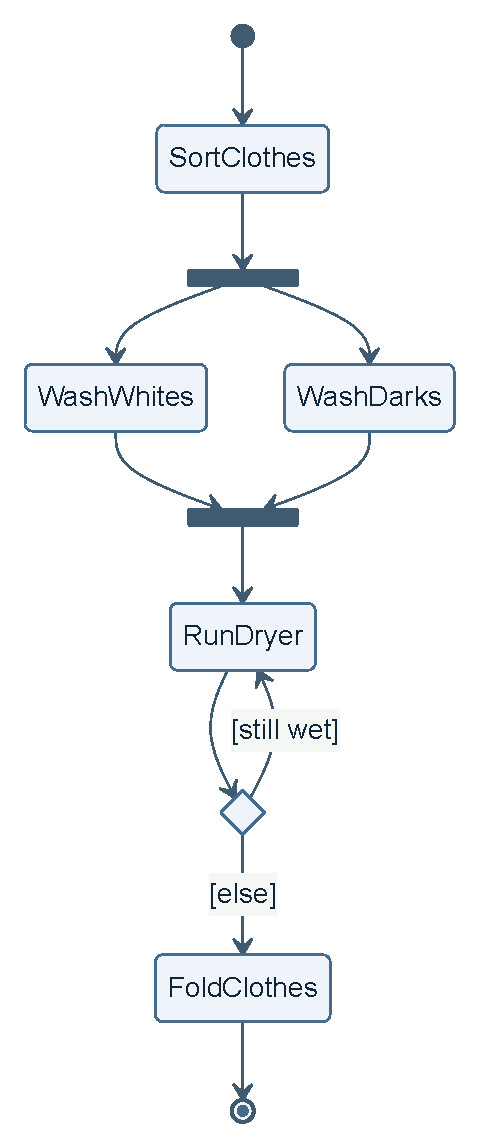
\includegraphics[width=125.48pt]{images/fig-019.pdf}
\captionof{figure}{5.2 Activity diagram}\end{minipage}\par\smallskip


\textbf{UML check:} use action nodes, initial/final nodes and guarded diamonds. A join waits for parallel inputs; a merge rejoins alternatives.
\end{studycolumns}

\Needspace{4\baselineskip}
\subsection*{5.3 State machine vs activity diagram (L6 comparison)}
\sectionlabel{h-53-state-machine-vs-activity-diagram-l6-comparison}


{\fontsize{9}{11}\selectfont
\begin{longtable}{L{\dimexpr 0.23178\linewidth-5.56pt\relax}L{\dimexpr 0.39810\linewidth-9.55pt\relax}L{\dimexpr 0.37012\linewidth-8.88pt\relax}}
\toprule
\rowcolor{ice}\textbf{} & \textbf{\textbf{State machine}} & \textbf{\textbf{Activity}} \\
\midrule\endfirsthead
\toprule\rowcolor{ice}\textbf{} & \textbf{\textbf{State machine}} & \textbf{\textbf{Activity}} \\
\midrule\endhead
\multicolumn{3}{r}{\scriptsize Continued on next page}\\\endfoot
\bottomrule\endlastfoot
Models & The \textbf{states} of a system/\allowbreak{}object and events that move it & The \textbf{workflow of activities} (a flow chart) \\
Node meaning & A stable condition & A unit of work \\
Focus & Event-driven \textbf{reactive} behaviour & Procedural \textbf{control flow}, concurrency \\
Typical use & UI navigation (dialog map), protocol/\allowbreak{}device states & Business process, algorithm, use-case flow \\
\end{longtable}
}


\begin{quote}\small\color{navy}
\textbf{Trap:} fork/\allowbreak{}join are \textbf{bars}; decision/\allowbreak{}merge are \textbf{diamonds}. A diamond for concurrency or a bar for a conditional branch uses the wrong notation.

\end{quote}


\subsection*{5.4 The requirements elicitation \& analysis activity diagram (memorise the loop)}
\sectionlabel{h-54-the-requirements-elicitation--analysis-activity-diagram-memorise-the-loop}



\par\smallskip\noindent\begin{minipage}{\linewidth}\centering
\begin{minipage}[t]{0.488\linewidth}\centering\scriptsize\textbf{1}\par\smallskip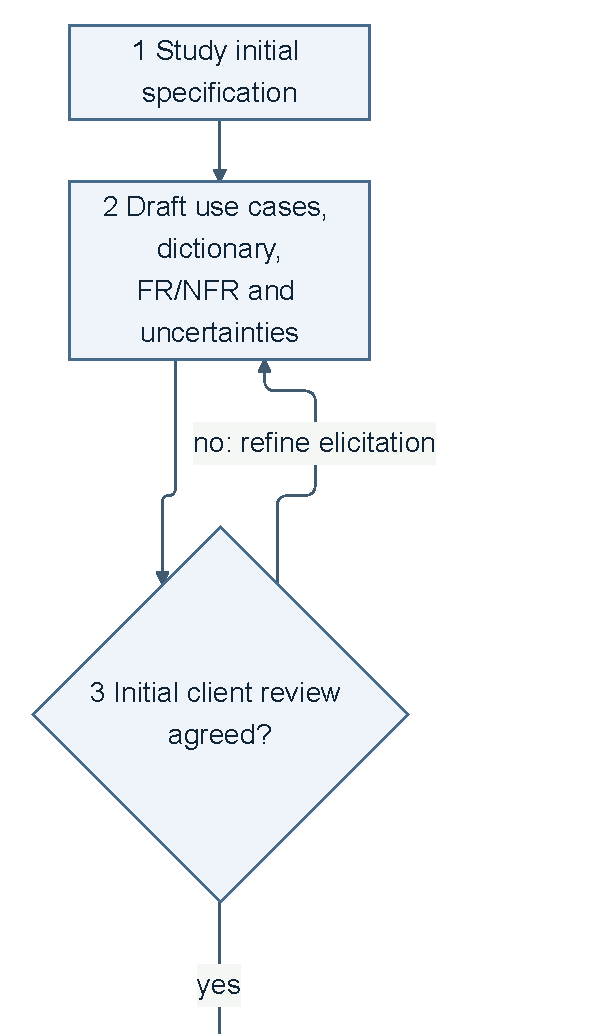
\includegraphics[width=177.48pt]{images/fig-020-compact-1.pdf}\end{minipage}\hfill
\begin{minipage}[t]{0.488\linewidth}\centering\scriptsize\textbf{2}\par\smallskip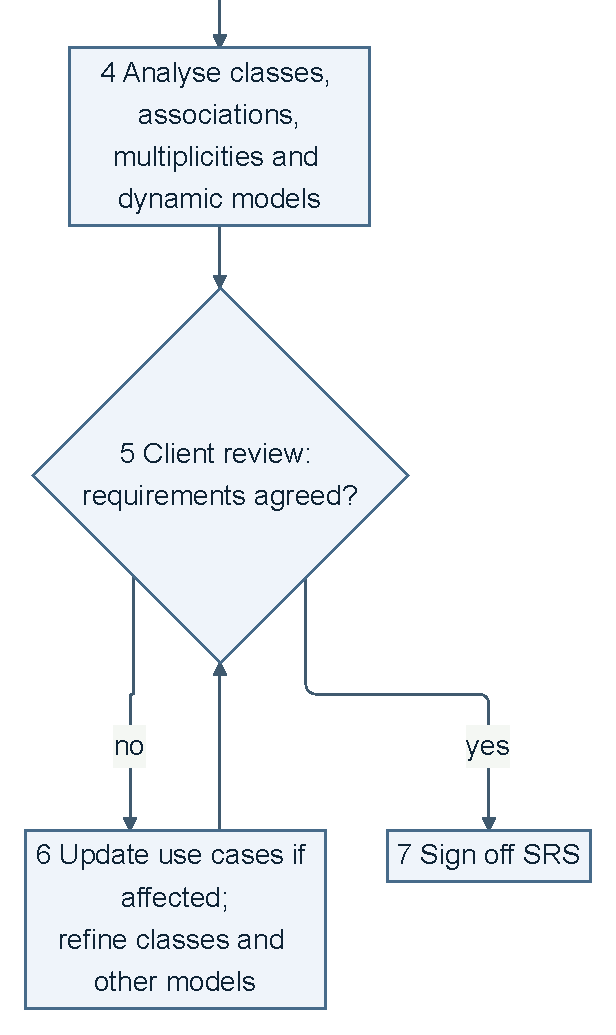
\includegraphics[width=177.48pt]{images/fig-020-compact-2.pdf}\end{minipage}
\captionof{figure}{5.4 The requirements elicitation \& analysis activity diagram --- follow numbered panels; crossing arrows continue.}\end{minipage}\par\smallskip




\chapteropen{Chapter 6: Software Requirements Specification}{chapter-6}
\markboth{Ch. 6 | SRS}{}


\begin{studycolumns}
\vspace{0pt}
\begin{eli5box}
An SRS is an agreement about the cake you ordered: size, flavour, delivery and how to check it. It should not secretly replace your order with the baker's preferred recipe. Someone reading the agreement should be able to tell whether the delivered product meets it.
\end{eli5box}
\textbf{Answer check:} Specify required behaviour, interfaces and qualities; leave arbitrary design choices out. Use identifiers plus trace links, measurable conditions and explicit TBDs. Adding ``shall'' alone does not repair an ambiguous requirement.
\end{studycolumns}

\subsection*{Visual: see the SRS as five compartments}
\sectionlabel{h-visual-see-the-srs-as-five-compartments}


\par\smallskip\noindent\begin{minipage}{\linewidth}\centering
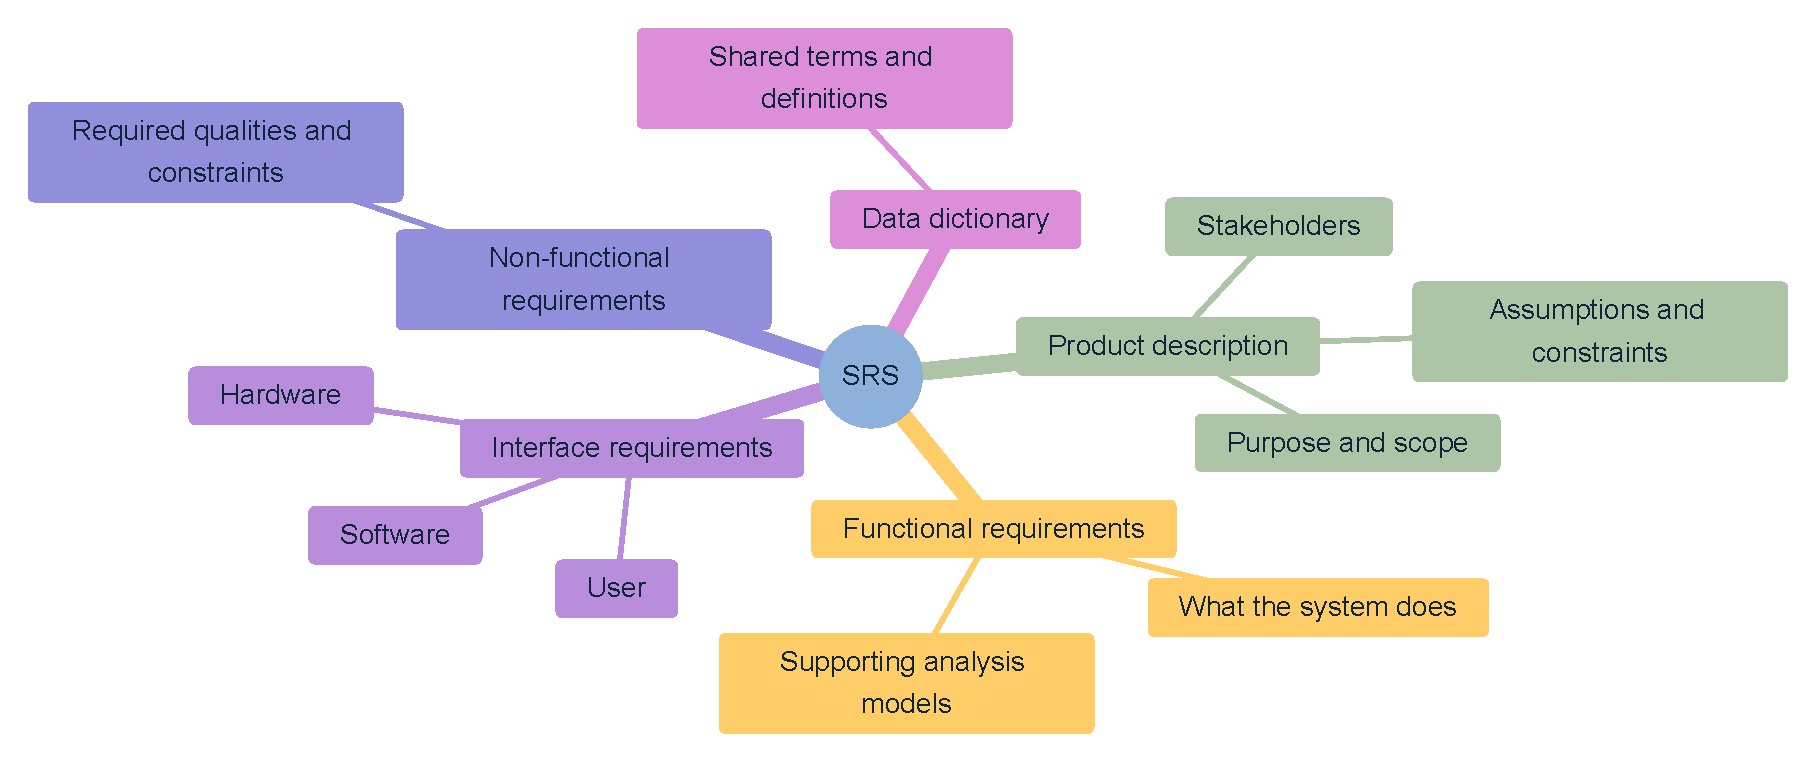
\includegraphics[width=514.00pt]{images/fig-021.pdf}
\captionof{figure}{see the SRS as five compartments}\end{minipage}\par\smallskip

\begin{studycolumns}
\vspace{0pt}



\needspace{4\baselineskip}
\subsection*{6.1 What the SRS is (six definitions that get paraphrased into exam questions)}
\sectionlabel{h-61-what-the-srs-is-six-definitions-that-get-paraphrased-into-exam-questions}
\begin{enumerate}
\item The \textbf{output of requirements elicitation and analysis}.
\item An organisation's \textbf{written understanding} of a customer's requirements and dependencies at a point in time, prior to design/\allowbreak{}development.
\item A \textbf{two-way insurance policy}: both client and organisation understand each other's requirements.
\item A statement in \textbf{precise, clear language} of the functions and capabilities the system must provide, plus required constraints.
\item A \textbf{blueprint} for completing the project with as little cost growth as possible.
\item \textbf{Detailed functional and non-functional requirements --- it does NOT contain design suggestions.}
\end{enumerate}
\needspace{4\baselineskip}
\subsection*{6.2 Purpose of the SRS (4 items)}
\sectionlabel{h-62-purpose-of-the-srs-4-items}
\begin{enumerate}
\item Give the customer assurance that the organisation understands the problems to be solved and the necessary software behaviour.
\item \textbf{Decompose} the problem into component parts.
\item Serve as \textbf{input to the design specification} --- so it must contain sufficient functional detail for a design solution to be devised.
\item Serve as the \textbf{parent/\allowbreak{}master document for testing and validation}.
\end{enumerate}
\end{studycolumns}

\Needspace{4\baselineskip}
\subsection*{6.3 Contents (5 sections --- memorise the numbering)}
\sectionlabel{h-63-contents-5-sections--memorise-the-numbering}


{\fontsize{9}{11}\selectfont
\begin{longtable}{L{\dimexpr 0.08684\linewidth-2.08pt\relax}L{\dimexpr 0.28102\linewidth-6.74pt\relax}L{\dimexpr 0.63214\linewidth-15.17pt\relax}}
\toprule
\rowcolor{ice}\textbf{Section } & \textbf{Section} & \textbf{Contents} \\
\midrule\endfirsthead
\toprule\rowcolor{ice}\textbf{Section } & \textbf{Section} & \textbf{Contents} \\
\midrule\endhead
\multicolumn{3}{r}{\scriptsize Continued on next page}\\\endfoot
\bottomrule\endlastfoot
1 & \textbf{Product description} & a) Purpose of the system (mission statement) \ensuremath{\cdot} b) Scope \ensuremath{\cdot} c) Users and stakeholders \ensuremath{\cdot} d) Assumptions and constraints \\
2 & \textbf{Functional requirements} & Precise numbered statements + activity diagrams, use case diagrams with descriptions, class diagrams, sequence diagrams, communication diagrams, state machine diagrams, UI prototype \\
3 & \textbf{Non-functional requirements} & Numbered statements covering performance, standards, reliability, availability, security, maintainability, portability \\
4 & \textbf{Interface requirements} & a) \textbf{User} (screen formats, layouts, report/\allowbreak{}menu content, function keys) \ensuremath{\cdot} b) \textbf{Hardware} (ports, instruction sets) \ensuremath{\cdot} c) \textbf{Software} (interfaces to DBMS, OS, maths packages) \\
5 & \textbf{Data dictionary} & Unambiguously defines all terms, phrases and abbreviations used in the SRS \\
\end{longtable}
}

Standards reference: \textbf{IEEE 830-1998}, \emph{IEEE Recommended Practice for Software Requirements Specifications}.

Who writes it: it should be in \textbf{natural language, unambiguous, with diagrams as necessary}; it must be understood by the development team; programmers/\allowbreak{}managers are seldom the best writers, so it is good practice to \textbf{involve a technical writer}.


\Needspace{4\baselineskip}
\subsection*{6.4 The nine language-quality characteristics}
\sectionlabel{h-64-the-nine-language-quality-characteristics}


{\fontsize{9}{11}\selectfont
\begin{longtable}{L{\dimexpr 0.11235\linewidth-2.70pt\relax}L{\dimexpr 0.28057\linewidth-6.73pt\relax}L{\dimexpr 0.60708\linewidth-14.57pt\relax}}
\toprule
\rowcolor{ice}\textbf{\#} & \textbf{Characteristic} & \textbf{Test you can apply} \\
\midrule\endfirsthead
\toprule\rowcolor{ice}\textbf{\#} & \textbf{Characteristic} & \textbf{Test you can apply} \\
\midrule\endhead
\multicolumn{3}{r}{\scriptsize Continued on next page}\\\endfoot
\bottomrule\endlastfoot
1 & \textbf{Correct} & Only user representatives can confirm; include them in inspections \\
2 & \textbf{Feasible} & Implementable within known capabilities/\allowbreak{}limits of system and environment \\
3 & \textbf{Necessary} & Can you identify its origin (customer need, external interface, standard)? If not, maybe not necessary \\
4 & \textbf{Unambiguous} & Multiple readers must reach \textbf{one} interpretation \\
5 & \textbf{Verifiable} & Can you devise a test /\allowbreak{} inspection /\allowbreak{} demonstration for it? \\
6 & \textbf{Complete} & Nothing missing; organise hierarchically so reviewers can spot gaps \\
7 & \textbf{Consistent} & No conflict with other requirements or higher-level requirements \\
8 & \textbf{Modifiable} & Uniquely labelled, expressed separately, change history maintained \\
9 & \textbf{Traceable} & Link each requirement to its source and its realisation \\
\end{longtable}
}

\begin{studycolumns}
\vspace{0pt}

\needspace{4\baselineskip}
\subsection*{6.5 Word list (memorise both columns)}
\sectionlabel{h-65-word-list-memorise-both-columns}
\textbf{YES Use these words}


\begin{referenceentries}
\textit{\textbf{YES Use} / \textbf{Meaning}}\par\smallskip
\noindent \textbf{\textbf{Shall}}: Dictates provision of a functional capability\par
\noindent \textbf{\textbf{Must /\allowbreak{} Must not}}: Establishes performance requirement or constraint\par
\noindent \textbf{\textbf{Is required to}}: Imperative in SRS statements\par
\noindent \textbf{\textbf{Are applicable}}: Includes standards/\allowbreak{}documentation by reference\par
\noindent \textbf{\textbf{Responsible for}}: Imperative for pre-defined architectures\par
\noindent \textbf{\textbf{Will}}: Cites what the operational/\allowbreak{}development \textbf{environment} will provide\par
\end{referenceentries}
\textbf{NO Avoid these words}


\begin{referenceentries}
\textit{\textbf{NO Avoid} / \textbf{Why}}\par\smallskip
\noindent \textbf{adequate}: vague threshold\par
\noindent \textbf{as a minimum}: unbounded\par
\noindent \textbf{be capable of\ldots{}}: avoids commitment\par
\noindent \textbf{as applicable /\allowbreak{} as appropriate}: optional\par
\noindent \textbf{effective}: unmeasurable\par
\noindent \textbf{if possible /\allowbreak{} if practical}: optional\par
\noindent \textbf{timely}: unmeasurable\par
\noindent \textbf{normal}: undefined baseline\par
\end{referenceentries}

\begin{quote}\small\color{navy}
The two lists are \textbf{independent} --- the lecture presents them side by side, so a row on the left is not the "opposite" of the row on the right.

\end{quote}

\begin{quote}\small\color{navy}
\textbf{Trap (shall vs will).} \textbf{Shall} binds the \emph{system}; \textbf{will} describes what the \emph{environment} supplies. "The system \textbf{shall} \ldots{}" is a requirement; "The user \textbf{will} provide a valid card" is an assumption about the environment. Swapping them blurs responsibility for the behaviour.


\end{quote}
\end{studycolumns}

\chapteropen{Chapter 7: Software process models}{chapter-7}
\markboth{Ch. 7 | Processes}{}


\begin{studycolumns}
\vspace{0pt}
\begin{eli5box}
Waterfall is like planning a whole house before construction; incremental delivery is like opening usable rooms in stages; reuse/\allowbreak{}configuration is like assembling suitable existing modules. None is automatically best. Choose according to change, risk, available components and the need for predictable agreement.
\end{eli5box}
\textbf{Answer check:} Choose using change, risk, component fit and constraints. Give a case-specific benefit and trade-off. Waterfall includes testing; agile includes planning. Customer involvement does not eliminate the cost of late change.
\end{studycolumns}

\subsection*{Visual: compare how the work is arranged}
\sectionlabel{h-visual-compare-how-the-work-is-arranged}


\par\smallskip\noindent\begin{minipage}{\linewidth}\centering
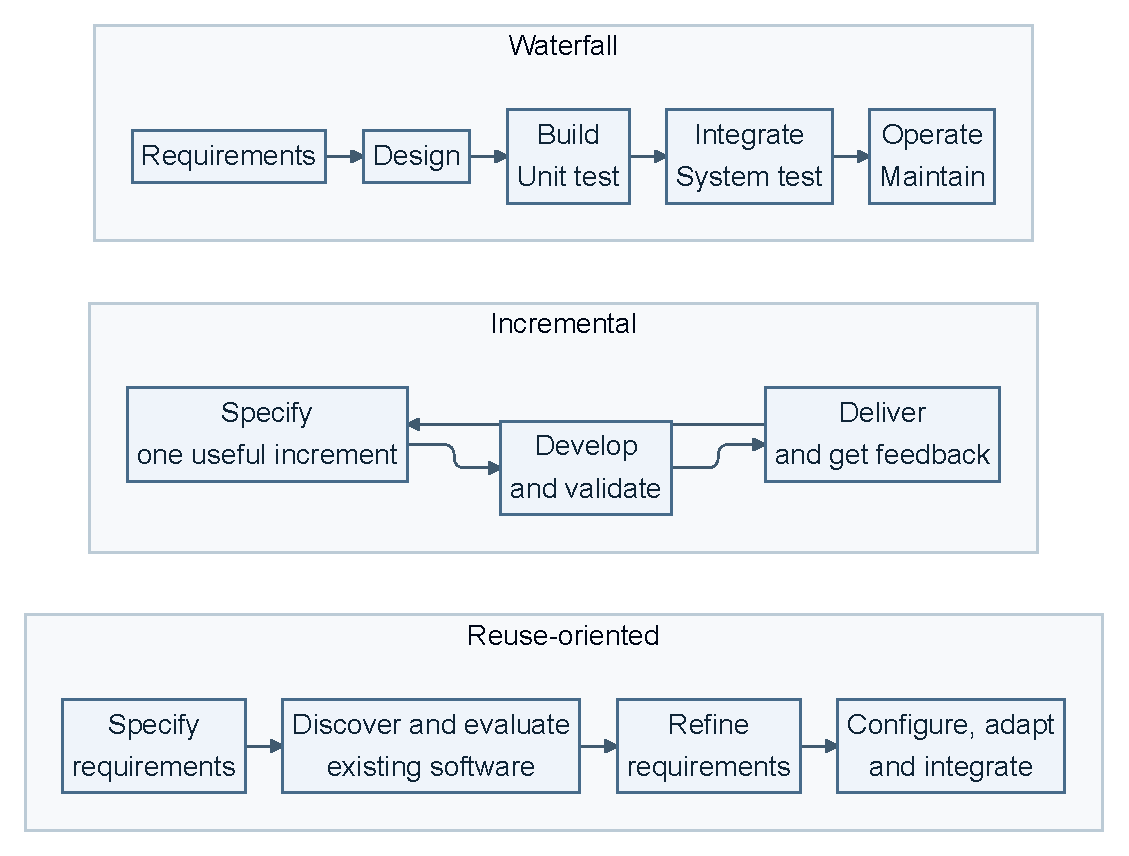
\includegraphics[width=332.12pt]{images/fig-022.pdf}
\captionof{figure}{compare how the work is arranged}\end{minipage}\par\smallskip

\begin{studycolumns}
\vspace{0pt}



\needspace{4\baselineskip}
\subsection*{7.1 Definitions}
\sectionlabel{h-71-definitions}

\begin{quote}\small\color{navy}
A \textbf{software process} is \emph{a structured set of activities required to develop a software system.}

\end{quote}
All processes involve specification, design/\allowbreak{}implementation, validation and evolution (Chapter 1). Their arrangement and feedback differ.

\begin{quote}\small\color{navy}
A \textbf{software process model} is \emph{an abstract representation of a process --- a description from some particular perspective.}

\end{quote}
\textbf{Process descriptions} include, besides activities and their ordering:

\begin{itemize}
\item \textbf{Products} --- outcomes of a process activity;
\item \textbf{Roles} --- responsibilities of the people involved;
\item \textbf{Pre- and post-conditions} --- statements true before/\allowbreak{}after an activity or product.
\end{itemize}
\end{studycolumns}

\Needspace{4\baselineskip}
\subsection*{7.2 Plan-driven vs agile}
\sectionlabel{h-72-plan-driven-vs-agile}


{\fontsize{9}{11}\selectfont
\begin{longtable}{L{\dimexpr 0.19914\linewidth-4.78pt\relax}L{\dimexpr 0.34730\linewidth-8.34pt\relax}L{\dimexpr 0.45356\linewidth-10.89pt\relax}}
\toprule
\rowcolor{ice}\textbf{} & \textbf{\textbf{Plan-driven}} & \textbf{\textbf{Agile}} \\
\midrule\endfirsthead
\toprule\rowcolor{ice}\textbf{} & \textbf{\textbf{Plan-driven}} & \textbf{\textbf{Agile}} \\
\midrule\endhead
\multicolumn{3}{r}{\scriptsize Continued on next page}\\\endfoot
\bottomrule\endlastfoot
Planning & All activities planned \textbf{in advance}; progress measured against the plan & Planning is \textbf{incremental}; process easily changed to reflect changing requirements \\
Iteration & Iteration occurs \textbf{within} activities & Specification, design, implementation, testing are \textbf{inter-leaved}; outputs negotiated during development \\
Outputs & Decided \textbf{up front} & Decided through \textbf{negotiation} during the process \\
\end{longtable}
}

Most practical processes include \textbf{elements of both}. \textbf{There are no right or wrong software processes.}


\Needspace{4\baselineskip}
\subsection*{7.3 The three general models}
\sectionlabel{h-73-the-three-general-models}


{\fontsize{9}{11}\selectfont
\begin{longtable}{L{\dimexpr 0.13392\linewidth-5.36pt\relax}L{\dimexpr 0.19287\linewidth-7.71pt\relax}L{\dimexpr 0.22020\linewidth-8.81pt\relax}L{\dimexpr 0.19571\linewidth-7.83pt\relax}L{\dimexpr 0.25730\linewidth-10.29pt\relax}}
\toprule
\rowcolor{ice}\textbf{Model} & \textbf{Shape} & \textbf{When used} & \textbf{Key benefit} & \textbf{Key problem} \\
\midrule\endfirsthead
\toprule\rowcolor{ice}\textbf{Model} & \textbf{Shape} & \textbf{When used} & \textbf{Key benefit} & \textbf{Key problem} \\
\midrule\endhead
\multicolumn{5}{r}{\scriptsize Continued on next page}\\\endfoot
\bottomrule\endlastfoot
\textbf{Waterfall} & Separate, distinct, sequential phases & Requirements \textbf{well understood} and changes limited; large systems-engineering projects developed at several sites & Plan-driven coordination across sites & \textbf{Difficulty of accommodating change} once under way; inflexible partitioning \\
\textbf{Incremental} & Specification, development, validation \textbf{inter-leaved}; may be plan-driven \textbf{or} agile & Most business systems & Lower cost of accommodating change; easier customer feedback; earlier delivery of value & \textbf{Process not visible} (managers need deliverables); \textbf{structure degrades} as increments are added unless you refactor \\
\textbf{Integration \& configuration (reuse-oriented)} & Assemble from existing components/\allowbreak{}COTS & Systems buildable from existing assets; standard for many business systems & Reduced cost and risk; faster delivery & \textbf{Requirements compromises inevitable}; loss of control over evolution of reused elements \\
\end{longtable}
}

\begin{studycolumns}
\vspace{0pt}

\textbf{Waterfall phases} (exact names): Requirements analysis and definition \ensuremath{\rightarrow} System and software design \ensuremath{\rightarrow} Implementation and unit testing \ensuremath{\rightarrow} Integration and system testing \ensuremath{\rightarrow} Operation and maintenance.


\textbf{Visibility note:} managers need regular deliverables, but documenting every version can be costly; refactoring controls the structural degradation identified in the table.

\textbf{Reuse-oriented phases (5):} requirements specification \ensuremath{\rightarrow} software discovery and evaluation \ensuremath{\rightarrow} requirements refinement \ensuremath{\rightarrow} application system configuration \ensuremath{\rightarrow} component adaptation and integration.

\textbf{Types of reusable software (3):} stand-alone application systems (COTS) configured for a particular environment; collections of objects packaged for a component framework (.NET, J2EE); web services developed to service standards and remotely invocable.


\begin{quote}\small\color{navy}
\textbf{Trap \#1.} "Incremental = agile" is \textbf{false} --- incremental development \emph{may be plan-driven}.


\end{quote}
\needspace{4\baselineskip}
\subsection*{7.4 Why costs are high /\allowbreak{} why maintenance dominates (Tutorial 4)}
\sectionlabel{h-74-why-costs-are-high--why-maintenance-dominates-tutorial-4}
Prepare a \emph{reasoned} answer, not a slogan:

\begin{itemize}
\item \textbf{Costs}: requirements churn, integration of heterogeneous components, testing effort grows super-linearly with interfaces, coordination cost in teams, environment/\allowbreak{}tooling/\allowbreak{}long lifetimes.
\item \textbf{Maintenance}: software is soft --- it \emph{can} change, so it \emph{must} change (new requirements, new platforms, bug fixes). Systems can live for decades; ongoing fixes and adaptation accumulate over that lifetime. Unlike hardware, there is no manufacturing cost, so evolution dominates total cost.
\item \textbf{Characteristics affecting development}: size (source/\allowbreak{}binary/\allowbreak{}users/\allowbreak{}developers/\allowbreak{}lifetime/\allowbreak{}versions), complexity (environment, technologies, hardware), cost and schedule constraints, non-functional requirements (performance, availability, security, scalability, extensibility).
\item \textbf{Two distinct differences from hardware manufacturing}: (1) software is \textbf{designed, not manufactured} --- copying is free; (2) software \textbf{does not wear out} --- it degrades by change, and hardware failures follow a bathtub curve.
\end{itemize}


\par\needspace{65pt}\phantomsection\label{answer-waterfall}
\textbf{Template W --- change/\allowbreak{}process answer:} clarify and record change; assess effects on requirements, design, code, tests, cost and schedule; agree revised scope/\allowbreak{}baselines; replan and verify. Early prototypes/\allowbreak{}reviews and increments expose change sooner, but do not remove late rework. Incremental delivery can be plan-driven or agile. For reuse, evaluate fixed-component fit, prototype risky integrations, negotiate acceptable compromises and isolate mismatches behind adapters.
\textbf{Comparison:} Waterfall favours stable baselines, sequential delivery and requirements/\allowbreak{}review/\allowbreak{}acceptance involvement; Agile favours reprioritised usable increments, frequent customer feedback and earlier adaptation.
\end{studycolumns}

\chapteropen{Chapter 8: Agile, XP and Scrum}{chapter-8}
\markboth{Ch. 8 | Agile and Scrum}{}


\begin{studycolumns}
\vspace{0pt}
\begin{eli5box}
A sprint is a short team promise to produce a usable increment and learn from it. The backlog is the prioritised queue; the Product Owner orders value; developers choose and organise feasible work; the Scrum Master helps the process work. Velocity is the team's measured delivery pace, not a demand to work faster.
\end{eli5box}
\textbf{Answer check:} Use the Sprint Goal, actual capacity and completed velocity. Developers retain ownership; the Scrum Master facilitates. Negotiate scope transparently instead of extending the timebox or lowering quality. Incomplete items earn no completed velocity.
\end{studycolumns}

\subsection*{Visual: follow one sprint through its feedback loops}
\sectionlabel{h-visual-follow-one-sprint-through-its-feedback-loops}


\par\smallskip\noindent\begin{minipage}{\linewidth}\centering
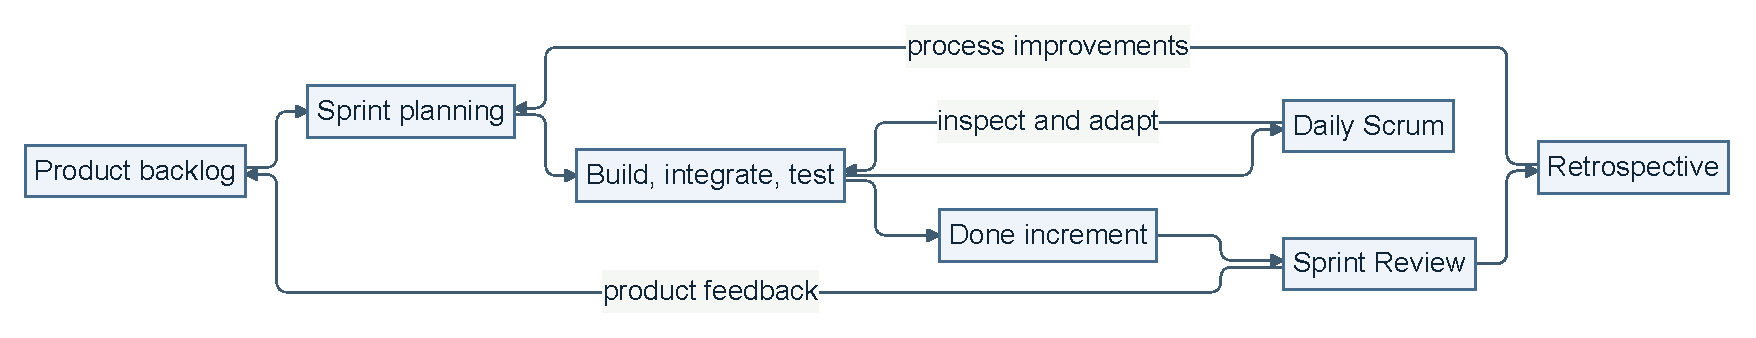
\includegraphics[width=514.00pt]{images/fig-023.pdf}
\captionof{figure}{follow one sprint through its feedback loops}\end{minipage}\par\smallskip

\begin{studycolumns}
\vspace{0pt}



\needspace{4\baselineskip}
\subsection*{8.1 Why agile emerged}
\sectionlabel{h-81-why-agile-emerged}
Rapid delivery became the dominant requirement: requirements change too fast for stable specs; plan-driven development does not meet these needs; agile methods (late 1990s) aimed to \textbf{radically reduce delivery time for working software}.

Agile development characteristics:

\begin{itemize}
\item program specification, design and implementation are \textbf{inter-leaved};
\item the system is developed as \textbf{a series of versions/\allowbreak{}increments}, with stakeholders involved in specification and evaluation of each version;
\item \textbf{frequent delivery} of new versions for evaluation;
\item \textbf{extensive tool support} (e.g. automated testing);
\item \textbf{minimal documentation} --- focus on working code.
\end{itemize}
\needspace{4\baselineskip}
\subsection*{8.2 Agile manifesto (4 values --- quote them exactly)}
\sectionlabel{h-82-agile-manifesto-4-values--quote-them-exactly}

\begin{quote}\small\color{navy}
We are uncovering better ways of developing software by doing it and helping others do it. Through this work we have come to value:

\begin{itemize}
\item \textbf{Individuals and interactions} over processes and tools
\item \textbf{Working software} over comprehensive documentation
\item \textbf{Customer collaboration} over contract negotiation
\item \textbf{Responding to change} over following a plan
\end{itemize}
That is, while there is value in the items on the right, we value the items on the left more.

\end{quote}
\textbf{Trap:} it does \textbf{not} say "no documentation". Both sides have value; the left is \emph{valued more}. Saying "agile means no documentation" is inconsistent with the manifesto.

\needspace{4\baselineskip}
\subsection*{8.3 The five agile principles}
\sectionlabel{h-83-the-five-agile-principles}

\begin{referenceentries}
\textit{\textbf{Principle} / \textbf{Description}}\par\smallskip
\noindent \textbf{\textbf{Customer involvement}}: Customers closely involved throughout; provide and prioritise requirements, evaluate iterations\par
\noindent \textbf{\textbf{Incremental delivery}}: Software developed in increments; customer specifies requirements for each increment\par
\noindent \textbf{\textbf{People, not process}}: Recognise and exploit team skills; let teams develop their own ways of working\par
\noindent \textbf{\textbf{Embrace change}}: Expect requirements to change; design to accommodate change\par
\noindent \textbf{\textbf{Maintain simplicity}}: Focus on simplicity in software and process; actively eliminate complexity\par
\end{referenceentries}
\textbf{Applicability:} product development (small/\allowbreak{}medium product for sale) and custom in-house development with a committed customer and few external rules/\allowbreak{}regulations.

\textbf{Across organisations:} managers may be risk-averse; large organisations have quality procedures incompatible with agile bureaucracy; agile works best with \textbf{high-skill teams} but large orgs have a wide skill range; cultural resistance where conventional processes are entrenched.

\needspace{4\baselineskip}
\subsection*{8.4 Extreme Programming (XP)}
\sectionlabel{h-84-extreme-programming-xp}
Extreme approach: new versions possibly \textbf{several times per day}; increments delivered \textbf{every 2 weeks}; \textbf{all tests run for every build}, and the build is accepted only if tests pass.

\textbf{Ten practices in L9, pp. 15--16:}


\begin{referenceentries}
\textit{\textbf{Practice} / \textbf{Description}}\par\smallskip
\noindent \textbf{\textbf{Incremental planning}}: Requirements on \textbf{story cards}; stories for a release chosen by time available and relative priority; developers break stories into \textbf{tasks}\par
\noindent \textbf{\textbf{Small releases}}: Minimal useful functionality providing business value first; releases frequent, adding functionality\par
\noindent \textbf{\textbf{Simple design}}: Enough design for current requirements and no more\par
\noindent \textbf{\textbf{Test-first development}}: Automated unit test framework; tests written \textbf{before} functionality\par
\noindent \textbf{\textbf{Refactoring}}: Continuous improvement of code as soon as improvements are found\par
\noindent \textbf{\textbf{Pair programming}}: Two developers at one machine, checking each other's work\par
\noindent \textbf{\textbf{Collective ownership}}: Pairs work on all areas; no islands of expertise; anyone can change anything\par
\noindent \textbf{\textbf{Continuous integration}}: Task integrated into the whole system as soon as complete; after any integration all unit tests must pass\par
\noindent \textbf{\textbf{Sustainable pace}}: Large amounts of overtime unacceptable --- reduces quality and medium-term productivity\par
\noindent \textbf{\textbf{On-site customer}}: A representative end-user available \textbf{full time}; a member of the team, responsible for bringing requirements\par
\end{referenceentries}
Related lecture topics: \textbf{user stories for specification} and \textbf{automated test harnesses}. These are not two extra entries in the ten-row practice table.

\textbf{Key influential practices (4):} user stories for specification, refactoring, test-first development, pair programming.

\textbf{XP refactoring check:} improve structure continuously because future changes are hard to predict; remove duplication and clarify responsibility. It improves understanding/\allowbreak{}changeability and can reduce documentation needs, but architectural refactoring is expensive.

\textbf{Pairing check:} rotating pairs share knowledge, ownership and informal review, reducing key-person risk and encouraging refactoring. Productivity gains are evidence-dependent, not guaranteed.

\textbf{TDD check:} executable, self-checking tests clarify requirements; run old and new tests after each addition for regression protection.


\begin{quote}\small\color{navy}
\textbf{Trap:} TDD \ensuremath{\neq} "testing at the end". TDD = test \textbf{first}, watch it fail, then implement. The "tests are written as programs rather than data" point is what makes automation possible.

\textbf{Trap:} XP is technically focused and \textbf{hard to integrate with management practice} in most organisations --- consequently the \emph{method as originally defined is not widely used}, even though its practices are.

\end{quote}
\needspace{4\baselineskip}
\subsection*{8.5 Scrum}
\sectionlabel{h-85-scrum}
Scrum focuses on \textbf{managing iterative development} rather than on specific technical practices. The following describes the supplied L9 slides; do not treat their historical terminology as a statement of the current Scrum standard. The slides themselves contain variants: p. 32 says no more than 7 developers; p. 41 says 5--9. Neither is needed to infer the headcount in Tutorial 5 Q6.

\textbf{Three phases:}

\begin{enumerate}
\item \textbf{Outline planning} --- establish general objectives, design the software architecture.
\item \textbf{Sprint cycles} --- each develops an increment.
\item \textbf{Project closure} --- wrap up, complete documentation (help frames, user manuals), assess lessons learned.
\end{enumerate}
\textbf{Terminology (memorise verbatim-ish):}


\begin{referenceentries}
\textit{\textbf{Term} / \textbf{Definition}}\par\smallskip
\noindent \textbf{\textbf{Development team}}: A \textbf{self-organising} group, \textbf{no more than 7 people}, responsible for developing the software and essential project documents\par
\noindent \textbf{\textbf{Potentially shippable product increment}}: The increment delivered from a sprint; ideally in a finished state needing no further work (e.g. testing) before inclusion in the final product --- \emph{in practice not always achievable}\par
\noindent \textbf{\textbf{Product backlog}}: A list of "to do" items the Scrum team must tackle: feature definitions, requirements, user stories, or supplementary tasks such as architecture definition or user documentation\par
\noindent \textbf{\textbf{Product owner}}: An individual (or small group) who identifies features/\allowbreak{}requirements, \textbf{prioritises} them, and continuously reviews the backlog to ensure the project meets critical business needs; may be a customer, product manager, or stakeholder representative\par
\noindent \textbf{\textbf{Scrum (meeting)}}: A \textbf{daily} meeting of the Scrum team reviewing progress and prioritising work for that day; ideally short, face-to-face, whole team\par
\noindent \textbf{\textbf{ScrumMaster}}: Ensures the Scrum process is followed, guides the team in effective use of Scrum, interfaces with the rest of the company, protects the team from outside interference. \textbf{Should NOT be thought of as a project manager} (the developers are adamant; others may disagree)\par
\noindent \textbf{\textbf{Sprint}}: A development iteration, usually \textbf{2--4 weeks}\par
\noindent \textbf{\textbf{Velocity}}: An estimate of how much product-backlog effort the team can cover in one sprint; basis for estimating what fits and for measuring improvement\par
\end{referenceentries}
\textbf{Sprint cycle:} fixed length 2--4 weeks \ensuremath{\rightarrow} planning starts from the \textbf{product backlog} \ensuremath{\rightarrow} \textbf{selection phase} (whole team + customer select features for the sprint) \ensuremath{\rightarrow} team self-organises and develops, \textbf{isolated from customer and organisation}, all communication channelled through the ScrumMaster, whose role is to \textbf{protect the team from external distractions} \ensuremath{\rightarrow} at the end, work reviewed and presented to stakeholders \ensuremath{\rightarrow} next sprint begins.

\textbf{Teamwork:} the Scrum Master facilitates impediment resolution and communication; the Daily Scrum makes progress, problems and next steps visible for short-term replanning.

\textbf{Benefits:} manageable chunks, adaptation to unstable needs, team visibility/\allowbreak{}communication, timely customer feedback, and trust/\allowbreak{}positive culture.

\textbf{Practical Scrum material (L9, pp. 38--61; some pages are image-only):}

\begin{itemize}
\item \textbf{Product backlog:} owned by the PO; ordered requirements/\allowbreak{}features/\allowbreak{}tasks for the product.
\item \textbf{Sprint backlog:} selected product backlog items \textbf{plus the plan} for delivering the increment and Sprint Goal; owned by the Development Team. The slides protect the selected sprint scope and goal, while task estimates and remaining work are updated daily. Unfinished work returns to the product backlog for reconsideration; it earns no completed velocity points.
\item \textbf{Product increment:} integrates Done work with previous increments; tested and potentially releasable. Potentially shippable does not mean a release must occur every sprint.
\item \textbf{Sprint planning:} PO presents ordered items; developers decide how much fits and how to build it. Tasks are estimated in hours (the slide suggests 1--16 hours); points size backlog items, not hours.
\item \textbf{Daily Scrum:} 15-minute time box; yesterday's progress, today's plan and impediments.
\item \textbf{Sprint Review:} inspect the product with stakeholders and revise the product backlog. The slide gives a time box of 1 hour per week of sprint length.
\item \textbf{Sprint Retrospective:} inspect people, process and tools; agree improvements and actions for the next sprint. The slide gives 45 minutes per week, after the Review.
\item \textbf{Burndown chart:} remaining work against time; compare actual progress with planned work.
\end{itemize}
\textbf{Good backlog = DEEP (L9, pp. 54--55; Tutorial 5 Q3):} \textbf{Detailed appropriately} (small, detailed near-term items; larger, less detailed later items), \textbf{Emergent} (continually changes), \textbf{Estimated} (effort estimates inform prioritisation), \textbf{Prioritised} (especially work for upcoming sprints). Refinement continuously adds detail, estimates and reprioritises items; p. 56 suggests up to 10\% of team time as a guideline.

\textbf{User stories (L9, pp. 57--61):} ``As a [role], I want [action], so that [benefit].'' An \textbf{epic} is a large body of work split into smaller stories. The \textbf{3Cs} are \textbf{Card} (intent), \textbf{Conversation} (shared understanding) and \textbf{Confirmation} (acceptance criteria). Acceptance criteria define when work is finished; they can be functional or non-functional. State intent, remain independent of implementation and avoid unnecessary design detail. INVEST below evaluates the story itself.
\end{studycolumns}

\Needspace{4\baselineskip}
\subsection*{8.6 INVEST (Tutorial 5 --- memorise)}
\sectionlabel{h-86-invest-tutorial-5--memorise}


{\fontsize{9}{11}\selectfont
\begin{longtable}{L{\dimexpr 0.27665\linewidth-6.64pt\relax}L{\dimexpr 0.27665\linewidth-6.64pt\relax}L{\dimexpr 0.44670\linewidth-10.72pt\relax}}
\toprule
\rowcolor{ice}\textbf{Letter} & \textbf{Meaning} & \textbf{Test} \\
\midrule\endfirsthead
\toprule\rowcolor{ice}\textbf{Letter} & \textbf{Meaning} & \textbf{Test} \\
\midrule\endhead
\multicolumn{3}{r}{\scriptsize Continued on next page}\\\endfoot
\bottomrule\endlastfoot
\textbf{I} & \textbf{Independent} & Can be developed/\allowbreak{}released without depending on another story \\
\textbf{N} & \textbf{Negotiable} & Detail is negotiated between team and PO, not fixed up-front \\
\textbf{V} & \textbf{Valuable} & Delivers value to a user/\allowbreak{}customer \\
\textbf{E} & \textbf{Estimable} & Team can size it \\
\textbf{S} & \textbf{Small} & Fits in a sprint \\
\textbf{T} & \textbf{Testable} & Has an oracle; can be verified \\
\end{longtable}
}

\begin{studycolumns}
\vspace{0pt}

\needspace{4\baselineskip}
\subsection*{8.7 Velocity \& cost arithmetic (Tutorial 5 Q6)}
\sectionlabel{h-87-velocity--cost-arithmetic-tutorial-5-q6}

\begin{quote}\small\color{navy}
Total backlog = \textbf{64 points}. Scrum Team = Product Owner + ScrumMaster + \textbf{6} developers = \textbf{8} people. Cost per member per sprint = \textbf{\$2K}. \textbf{8 sprints} needed.

\end{quote}

\begin{ReferenceCode}
Velocity  = total points / number of sprints = 64 / 8 = 8 points per sprint
Cost      = people * cost per person per sprint * sprints
          = 8 * $2,000 * 8 = $128,000
\end{ReferenceCode}

\begin{quote}\small\color{navy}
\textbf{Trap:} do \textbf{not} drop the PO and ScrumMaster. The question says \emph{"each member in the Scrum Team"} and then enumerates them. Dropping them gives 6 \ensuremath{\times} 2K \ensuremath{\times} 8 = \textbf{\$96,000} (wrong). State your assumption explicitly if you think the question is ambiguous --- make the calculation auditable.

\textbf{New-team velocity:} use a trial sprint/\allowbreak{}history from comparable work as a provisional estimate, then measure completed points and adjust for capacity. It is not assigned hours or a mandated deadline.

\end{quote}


\par\needspace{65pt}\phantomsection\label{answer-scrum}
\textbf{Template S --- Scrum scenario answer:} identify the Sprint Goal and customer value; use completed velocity/\allowbreak{}real capacity; expose impediments and let developers solve technical work; PO/\allowbreak{}developers negotiate scope while protecting quality and timebox; review/\allowbreak{}retrospect and adapt. Forecast remaining sprints = remaining effort /\allowbreak{} representative velocity. Split oversized stories; investigate dependencies early. Urgent work normally enters a future backlog; only the PO cancels an obsolete goal. A Done increment is tested, integrated and potentially shippable.
\end{studycolumns}

\chapteropen{Chapter 9: Architecture and system design}{chapter-9}
\markboth{Ch. 9 | Architecture}{}


\begin{studycolumns}
\vspace{0pt}
\begin{eli5box}Architecture is a map of major parts and their communication. Choose the map using the case's important qualities and constraints.\end{eli5box}
\textbf{Answer check:} State the NFR, draw components/\allowbreak{}connectors, explain the mechanism, then name a cost or failure mode.
\needspace{326pt}
\subsection*{Visual: recognise the architectural organisation}
\sectionlabel{h-visual-recognise-the-architectural-organisation}
\par\smallskip\noindent\begin{minipage}{\linewidth}\centering
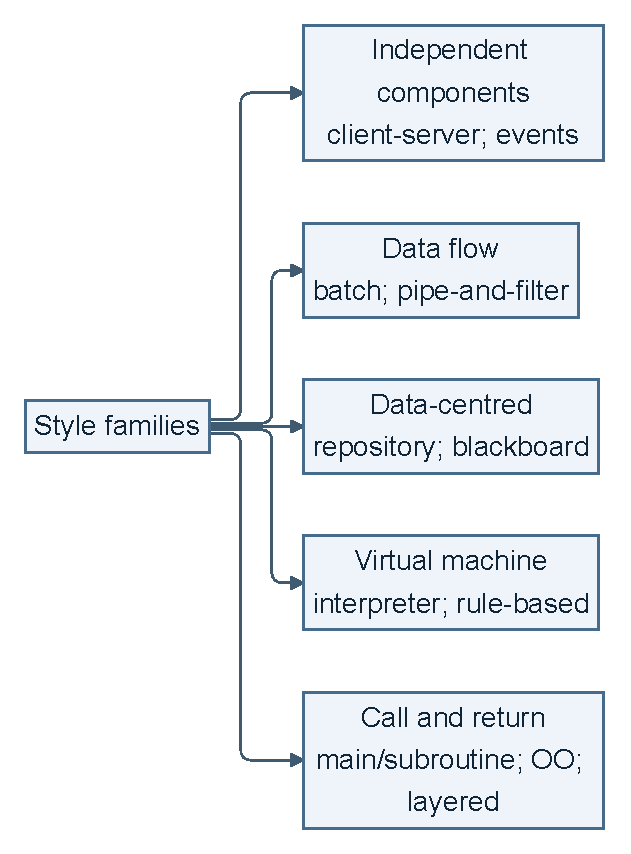
\includegraphics[width=185.38pt]{images/fig-024.pdf}
\captionof{figure}{recognise the architectural organisation}\end{minipage}\par\smallskip
\subsection*{9.1 Why design is hard here}
\sectionlabel{h-91-why-design-is-hard-here}
Scale, users, developers, versions, long lifetimes and changing technology increase complexity; cost, schedule, maintenance and NFRs constrain choices.
\subsection*{9.2 Definition}
\sectionlabel{h-92-definition}
\textbf{Architecture = components + connectors + constraints.} It abstracts implementation details, shows structure/\allowbreak{}interactions and demonstrates properties of interest. Connectors can be distributed across components rather than exist as separate runtime objects.
\end{studycolumns}


{\fontsize{9}{11}\selectfont
\begin{longtable}{L{\dimexpr 0.19355\linewidth-4.65pt\relax}L{\dimexpr 0.38710\linewidth-9.29pt\relax}L{\dimexpr 0.41935\linewidth-10.06pt\relax}}
\toprule
\rowcolor{ice}\textbf{} & \textbf{Definition} & \textbf{Examples} \\
\midrule\endfirsthead
\toprule\rowcolor{ice}\textbf{} & \textbf{Definition} & \textbf{Examples} \\
\midrule\endhead
\multicolumn{3}{r}{\scriptsize Continued on next page}\\\endfoot
\bottomrule\endlastfoot
\textbf{Component} & A unit of software that performs some function \textbf{at run time} & programs, objects, processes, clients, servers, databases \\
\textbf{Connector} & Interaction among components: communication, coordination or cooperation & shared variable access, procedure calls, RPC, communication protocols, data streams, transaction streams \\
\end{longtable}
}

\begin{studycolumns}
\vspace{0pt}
\subsection*{9.3 Architectural style}
\sectionlabel{h-93-architectural-style}
A style defines a family through component/\allowbreak{}connector vocabulary, composition constraints and semantic models. Instances can vary in count, interaction mechanism and component function. Event systems use implicit or explicit invocation; styles may coexist.
\subsection*{9.5 Layered architecture}
\sectionlabel{h-95-layered-architecture}
Upper layers call lower services. Benefits: abstraction, extension and lower-layer reuse. Costs: traversal overhead, difficult layer boundaries and poor fit for some systems. A direct lower-to-concrete-upper callback breaks the dependency direction; Observer abstracts that up-call.
\subsection*{9.6 Client--server}
\sectionlabel{h-96-clientserver}
Separate client/\allowbreak{}server computation supports concurrency, scalability, integration and change. Network protocols must handle delivery, failure and coordination; correctness is harder than a local call.
\subsection*{9.7 Pipe-and-filter}
\sectionlabel{h-97-pipe-and-filter}
Filters transform streams through pipes without shared state. Good for batch/\allowbreak{}stream transformations; weak for interactive shared-state behaviour.
\subsection*{9.8 Data-centred (repository /\allowbreak{} blackboard)}
\sectionlabel{h-98-data-centred-repository--blackboard}
Components communicate through a central repository/\allowbreak{}blackboard. It integrates independently changing producers/\allowbreak{}consumers, but creates shared coupling, contention and a potential single failure point.
\end{studycolumns}

\subsection*{9.9 Design principles (L12 and L14)}
\sectionlabel{h-99-design-principles-l12-and-l14}

{\fontsize{9}{11}\selectfont
\begin{longtable}{L{.27\linewidth}L{.66\linewidth}}
\toprule\rowcolor{ice}\textbf{Principle} & \textbf{Rule and failure check}\\\midrule\endhead
SRP /\allowbreak{} high cohesion & One reason to change; related responsibilities stay together. A God class or input parser that also writes the database fails this check.\\
OCP /\allowbreak{} identify variation & Encapsulate what varies; extend behind a stable contract. A type-switch scattered through clients forces modification.\\
Interfaces /\allowbreak{} low coupling & Depend on abstractions and minimise cross-module dependencies; avoid fields tied to concrete vendors.\\
DRY & Keep one authoritative representation of knowledge; duplicated creation logic is a warning.\\
Least Knowledge & Talk to immediate collaborators; avoid chains such as a.getB().getC().doIt().\\
Separation /\allowbreak{} modularity & Separate UI, rules and data; use abstraction and modular boundaries to support reuse. Business rules in event handlers defeat this.\\
Composition over inheritance & Assemble behaviour rather than grow fragile subclass hierarchies.\\\bottomrule
\end{longtable}}

\begin{studycolumns}
\vspace{0pt}

\needspace{321pt}
\subsection*{9.10 Design rationale frame (design rationale)}
\sectionlabel{h-910-design-rationale-frame-design-rationale}
\par\smallskip\noindent\begin{minipage}{\linewidth}\centering
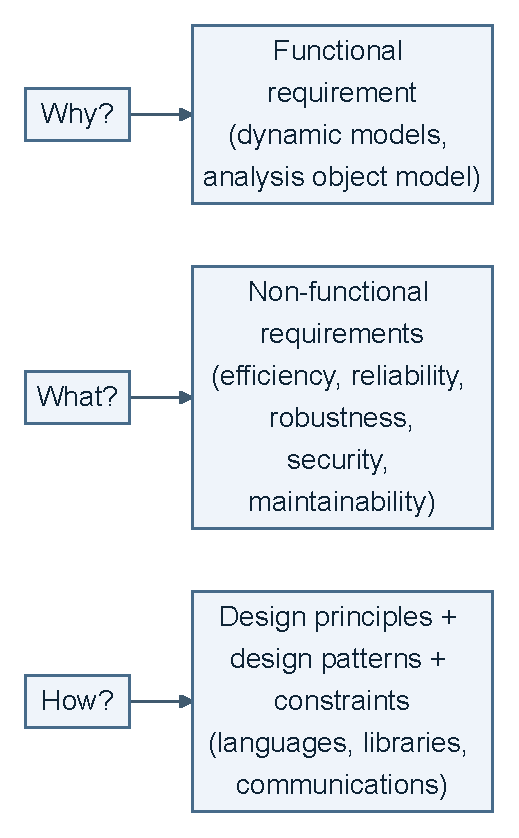
\includegraphics[width=152.26pt]{images/fig-025.pdf}
\captionof{figure}{9.10 Design rationale frame (design rationale)}\end{minipage}\par\smallskip
\par\needspace{65pt}\phantomsection\label{answer-architecture}
\textbf{Template A --- architecture justification:} [case NFR and why it matters]; [style, components and connectors]; [mechanism supporting the NFR]; [cost/\allowbreak{}failure mode and assumption]. Compare alternatives against the same requirement/\allowbreak{}workload; class or edge count alone is not quality evidence.
\subsection*{9.11 The design process (descriptive model)}
\sectionlabel{h-911-the-design-process-descriptive-model}
Model requirements; propose alternatives; validate against requirements; revise mismatches; elaborate, compare and select a blueprint.
\end{studycolumns}

\chapteropen{Chapter 10: Object design and design patterns}{chapter-10}
\markboth{Ch. 10 | Design patterns}{}

\begin{eli5box}Strategy changes behaviour; Factory creates the chosen object; Observer tells subscribers about changes; Facade offers one simple entry point.\end{eli5box}
\textbf{Answer check:} Name the problem and variation, map roles to the case, show relationships, then give a benefit and cost.
\subsection*{Pattern selection at a glance}


{\fontsize{9}{11}\selectfont
\begin{longtable}{L{.17\linewidth}L{.76\linewidth}}
\toprule\rowcolor{ice}\textbf{Pattern} & \textbf{Use when /\allowbreak{} mechanism /\allowbreak{} cost}\\\midrule\endhead
Strategy & Behaviour/\allowbreak{}algorithm varies; Context delegates to a stable interface. Extra indirection and selection.\\
Factory & Concrete type is known at runtime; centralise creation. Selection/\allowbreak{}configuration still needs maintenance.\\
Observer & Subscribers change over time; attach/\allowbreak{}detach/\allowbreak{}notify through an abstraction. Order, overhead and lifecycle cleanup matter.\\
Fa\c{c}ade & A subsystem is complex; offer one higher-level entry point. Poor/\allowbreak{}excessive facades add rework and overhead.\\\bottomrule
\end{longtable}}

\begin{studycolumns}
\vspace{0pt}

\subsection*{10.1 What object design adds over system design}
\sectionlabel{h-101-what-object-design-adds-over-system-design}
\begin{referenceentries}
\textit{\textbf{System design} / \textbf{Object design}}\par\smallskip
\noindent \textbf{System design:} Architecture, subsystems, layers, styles\par
\noindent \textbf{Object design:} \textbf{Detailed} class diagram, interfaces, patterns\par\smallskip
\noindent \textbf{System design:} Decides \emph{where} responsibility lives\par
\noindent \textbf{Object design:} Decides \emph{how} objects collaborate\par\smallskip
\end{referenceentries}\textbf{Object-design activities:} reuse; interface specification (operations, arguments, types, exceptions); restructuring for design goals; speed/\allowbreak{}memory optimisation.
\subsection*{10.2 Why patterns at all?}
\sectionlabel{h-102-why-patterns-at-all}
A pattern names a reusable response to recurring design forces. Its mechanism and consequences matter more than its name.
\subsection*{10.3 The four elements (L13 definition)}
\sectionlabel{h-103-the-four-elements-l13-definition}
\textbf{Name; problem; solution; consequences.} State when it applies, collaborating roles/\allowbreak{}relationships, and the resulting benefits/\allowbreak{}costs.
\subsection*{10.4 GoF 23 --- grouping (know the buckets)}
\sectionlabel{h-104-gof-23--grouping-know-the-buckets}
\begin{referenceentries}
\textit{\textbf{Category} / \textbf{Patterns}}\par\smallskip
\noindent \textbf{\textbf{Creational (5)}}: Abstract Factory, Builder, \textbf{Factory Method}, Prototype, \textbf{Singleton}\par
\noindent \textbf{\textbf{Structural (7)}}: Adapter, Bridge, Composite, \textbf{Decorator}, \textbf{Fa\c{c}ade}, Flyweight, Proxy\par
\noindent \textbf{\textbf{Behavioural (11)}}: Chain of Responsibility, \textbf{Command}, Interpreter, Iterator, Mediator, Memento, \textbf{Observer}, State, \textbf{Strategy}, Template Method, Visitor\par
\end{referenceentries}\subsection*{10.5 Strategy}
\sectionlabel{h-105-strategy}
\textbf{Strategy:} Context holds the Strategy abstraction and delegates operation(). Concrete strategies implement interchangeable behaviour, selected at runtime. Benefit: independent extension/\allowbreak{}encapsulation. Cost: indirection and a selection decision. The Factory below is optional when Strategy alone suffices.
\end{studycolumns}


\par\smallskip\noindent\begin{minipage}{\linewidth}\centering
\phantomsection\label{shared-pattern}
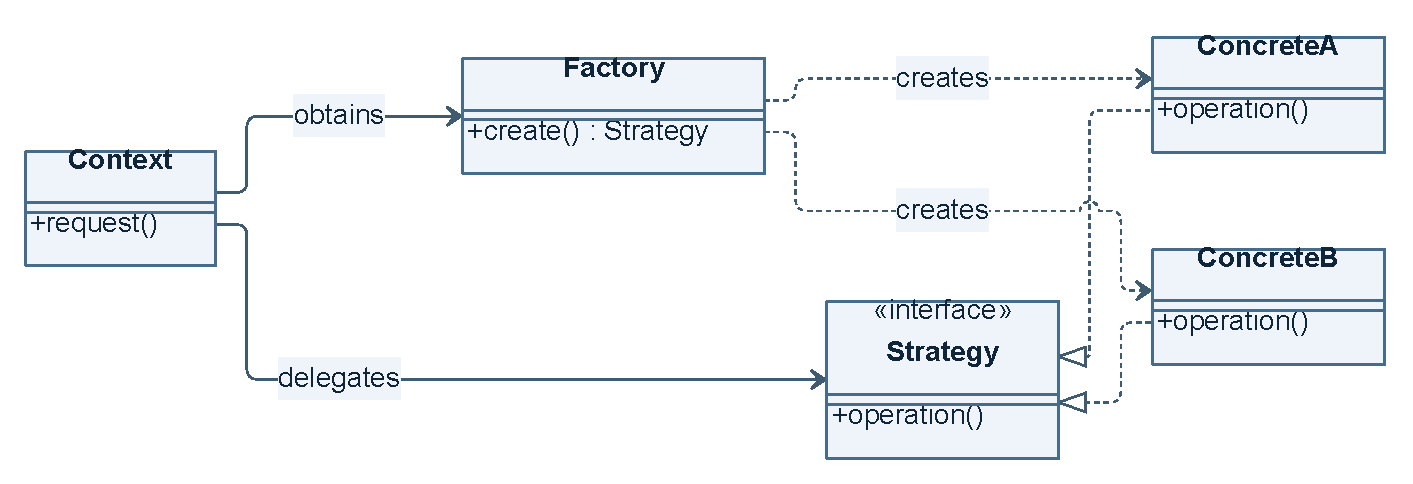
\includegraphics[width=440pt]{images/shared-strategy-factory.pdf}
\captionof{figure}{Canonical Strategy + Factory: substitute the paper's case roles. Factory creates; Context delegates.}\end{minipage}\par\smallskip

\begin{studycolumns}
\vspace{0pt}

\textbf{Template P --- combined-pattern answer:} identify independent behaviour and creation variation; map Context, Strategy, Factory and concrete implementations; show create and delegate relationships; explain extension behind a stable interface plus indirection/\allowbreak{}configuration cost. A switch-based factory still changes for a new type; registration/\allowbreak{}configuration or dynamic loading can move selection out of client code.
\subsection*{10.6 Observer (L13; Tutorial 7)}
\sectionlabel{h-106-observer-l13-tutorial-7}
\textbf{Observer:} Subject holds subscribers through the Observer abstraction; attach/\allowbreak{}detach manage membership, notify calls update. Runtime subscribers and selective interests decouple publisher from concrete listeners; callbacks or messages avoid blind polling. Also called Subscriber--Publisher or Consumer--Producer.
\end{studycolumns}


\par\smallskip\noindent\begin{minipage}{\linewidth}\centering
\begin{minipage}[t]{0.488\linewidth}\centering\scriptsize\textbf{1}\par\smallskip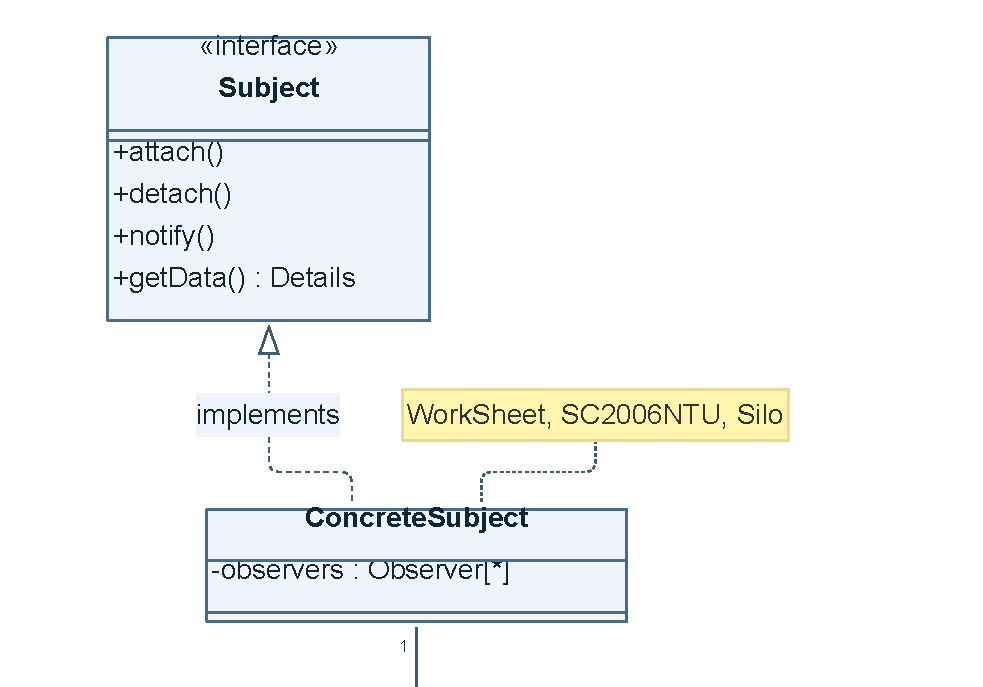
\includegraphics[width=251.00pt]{images/fig-029-compact-1.pdf}\end{minipage}\hfill
\begin{minipage}[t]{0.488\linewidth}\centering\scriptsize\textbf{2}\par\smallskip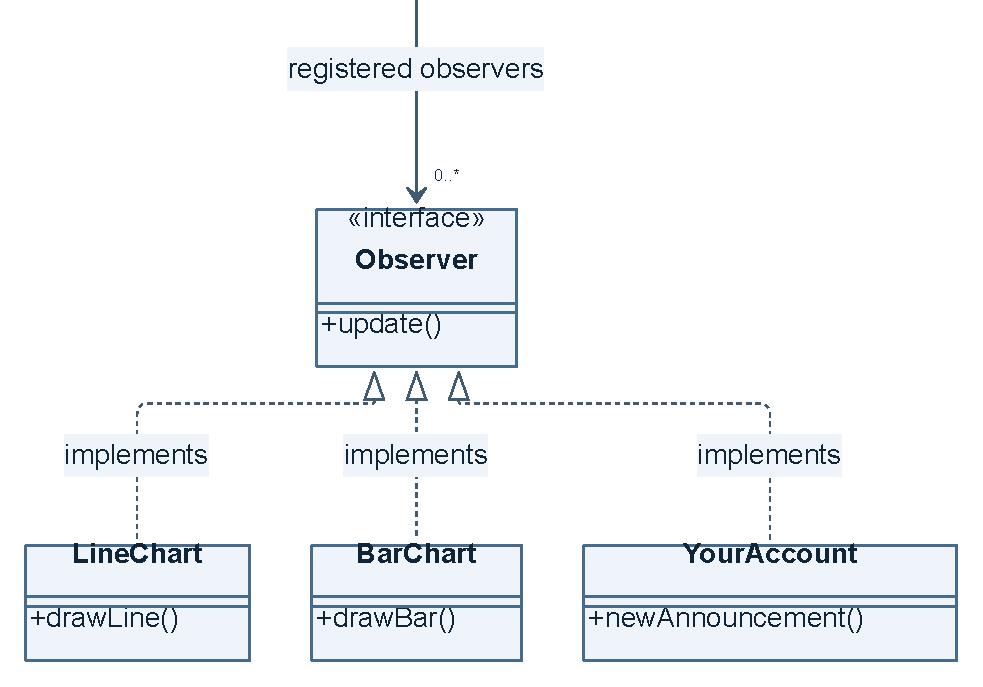
\includegraphics[width=251.00pt]{images/fig-029-compact-2.pdf}\end{minipage}
\captionof{figure}{10.6 Observer (L13; Tutorial 7) --- follow numbered panels; crossing arrows continue.}\end{minipage}\par\smallskip



{\fontsize{9}{11}\selectfont
\begin{longtable}{L{\dimexpr 0.23448\linewidth-5.63pt\relax}L{\dimexpr 0.37198\linewidth-8.93pt\relax}L{\dimexpr 0.39353\linewidth-9.44pt\relax}}
\toprule
\rowcolor{ice}\textbf{} & \textbf{\textbf{Pull}} & \textbf{\textbf{Push}} \\
\midrule\endfirsthead
\toprule\rowcolor{ice}\textbf{} & \textbf{\textbf{Pull}} & \textbf{\textbf{Push}} \\
\midrule\endhead
\multicolumn{3}{r}{\scriptsize Continued on next page}\\\endfoot
\bottomrule\endlastfoot
Subject sends & Simple notification (\code{update()}) & Detailed change data (\code{update(data)}) \\
Observer then & Calls back \code{get\allowbreak{}Data()} --- \textbf{two-way} & Needs no callback --- \textbf{one-way} \\
Coupling & Observer must know the subject's getters & Subject must know what observers need; may over-send \\
Efficiency & Observer fetches only if interested & Wastes data when observer is uninterested \\
\end{longtable}
}

\begin{studycolumns}
\vspace{0pt}
\textbf{Trade-off:} independent reuse and broadcast versus notification overhead, update storms, unspecified order and subscription-cleanup leaks. Selective notification filters registered interests; either push or pull can be used.
\subsection*{10.7 Factory (Static Factory)}
\sectionlabel{h-107-factory-static-factory}
\textbf{Simple/\allowbreak{}Static Factory} centralises runtime selection and construction, removes duplicate creation code and can provide lazy or singleton instances. It differs from GoF Factory Method (subclass-overridden creation) and Abstract Factory (families of related products).

\textbf{Examples:} JDBC creates vendor-specific Connections; Swing selects Look\&Feel; Eclipse loads registered ViewPart subclasses. Dynamic loading supports new configured classes without hard-coding them in the client. Construction remains a separate responsibility from Strategy delegation.
\subsection*{10.8 Fa\c{c}ade}
\sectionlabel{h-108-façade}
\textbf{Fa\c{c}ade} provides a unified higher-level interface to a subsystem. It reduces client dependencies and simplifies use. Costs: a poor facade needs rework; excessive facades add complexity/\allowbreak{}overhead. Direct subsystem access can still exist. Adapter instead converts an incompatible interface.
\end{studycolumns}

\subsection*{10.9 Other patterns you must be able to \emph{name} for a scenario}
\sectionlabel{h-109-other-patterns-you-must-be-able-to-_name_-for-a-scenario}

{\fontsize{9}{11}\selectfont
\begin{longtable}{L{\dimexpr 0.22481\linewidth-5.40pt\relax}L{\dimexpr 0.45466\linewidth-10.91pt\relax}L{\dimexpr 0.32053\linewidth-7.69pt\relax}}
\toprule
\rowcolor{ice}\textbf{Pattern} & \textbf{Scenario signal} & \textbf{Sketch} \\
\midrule\endfirsthead
\toprule\rowcolor{ice}\textbf{Pattern} & \textbf{Scenario signal} & \textbf{Sketch} \\
\midrule\endhead
\multicolumn{3}{r}{\scriptsize Continued on next page}\\\endfoot
\bottomrule\endlastfoot
\textbf{Singleton} & "exactly one instance", configuration/\allowbreak{}registry, lazy init & private ctor, static \code{get\allowbreak{}Instance()} \\
\textbf{Abstract Factory} & "create \textbf{families} of related objects" (controller \emph{or} look-and-feel for a view) & \code{Abstract\allowbreak{}Factory.\allowbreak{}create\allowbreak{}Button()/\allowbreak{}create\allowbreak{}Menu()} \\
\textbf{Factory Method} & Subclasses decide which class to instantiate & \code{creator.\allowbreak{}factory\allowbreak{}Method()} \\
\textbf{DAO} & Isolate persistence from domain logic & \code{Customer\allowbreak{}DAO.\allowbreak{}find(id)} \\
\textbf{Decorator} & Attach \textbf{additional} responsibilities dynamically (e.g. scrolling on a view) & \code{Scrolling\allowbreak{}View wraps View} \\
\textbf{Composite} & Nested views (Panel contains Button; nested Panels) & tree of \code{Component} \\
\textbf{Command} & Undo/\allowbreak{}redo of user actions & \code{Command.\allowbreak{}execute()/\allowbreak{}undo()} \\
\textbf{Adapter} & Convert one interface into another expected by the client & wrapper class \\
\textbf{Proxy} & Surrogate controlling access (remote/\allowbreak{}lazy/\allowbreak{}protection) & same interface as real subject \\
\end{longtable}
}
\par\Needspace{65pt}\phantomsection\label{answer-pattern-cost}
\textbf{Template C --- combine/\allowbreak{}criticise patterns:} combine only for distinct compatible forces; shared classes may play several roles if responsibilities stay clear. Give one concrete benefit and one cost (interfaces, indirection, lifecycle/\allowbreak{}configuration or tests). MVC combines Observer and Strategy; a smaller design can be preferable when variation is absent.

\chapteropen{Chapter 11: Model-View-Controller}{chapter-11}
\markboth{Ch. 11 | MVC}{}


\begin{studycolumns}
\vspace{0pt}
\begin{eli5box}One spreadsheet Model can feed a table and chart. Controllers interpret input; a Model change notifies Views so they refresh consistently.\end{eli5box}
\textbf{Answer check:} Trace input, Model update, notification and View refresh. MVC is triangular; it can coexist with layered services/\allowbreak{}persistence.
\subsection*{11.1 The problem MVC solves}
\sectionlabel{h-111-the-problem-mvc-solves}
Use MVC for interactive systems with changing input/\allowbreak{}display behaviour and multiple synchronised views of shared information. It separates presentation and interaction from core rules/\allowbreak{}data.
\end{studycolumns}

\subsection*{11.2 Components}
\sectionlabel{h-112-components}

{\fontsize{9}{11}\selectfont
\begin{longtable}{L{\dimexpr 0.15756\linewidth-5.04pt\relax}L{\dimexpr 0.46161\linewidth-14.77pt\relax}L{\dimexpr 0.17616\linewidth-5.64pt\relax}L{\dimexpr 0.20468\linewidth-6.55pt\relax}}
\toprule
\rowcolor{ice}\textbf{Component} & \textbf{Responsibility} & \textbf{Stereotype} & \textbf{Example} \\
\midrule\endfirsthead
\toprule\rowcolor{ice}\textbf{Component} & \textbf{Responsibility} & \textbf{Stereotype} & \textbf{Example} \\
\midrule\endhead
\multicolumn{4}{r}{\scriptsize Continued on next page}\\\endfoot
\bottomrule\endlastfoot
\textbf{Model} & Contains the \textbf{processing (operations) and the data} & \guillemotleft{}control\guillemotright{} + \guillemotleft{}entity\guillemotright{} & \code{Work\allowbreak{}Sheet}, \code{Sheet\allowbreak{}Manager} \\
\textbf{View} & Defines and manages \textbf{how data is presented}; each View provides a specific presentation of the same Model; each View \textbf{observes} the Model & \guillemotleft{}boundary\guillemotright{} & \code{Line\allowbreak{}Chart}, \code{Bar\allowbreak{}Chart} \\
\textbf{Controller} & Manages \textbf{user interaction}: captures input (mouse clicks, key presses) and passes interactions to View and Model; each View is associated with a Controller; user interacts \textbf{solely through Controllers} & \guillemotleft{}boundary\guillemotright{}/\allowbreak{}\guillemotleft{}control\guillemotright{} & \code{Edit\allowbreak{}WS}, \code{Edit\allowbreak{}WSCtrler} \\
\end{longtable}
}

\subsection*{11.3 The triangular structure (know the arrows by heart)}
\sectionlabel{h-113-the-triangular-structure-know-the-arrows-by-heart}

\par\smallskip\noindent\begin{minipage}{\linewidth}\centering
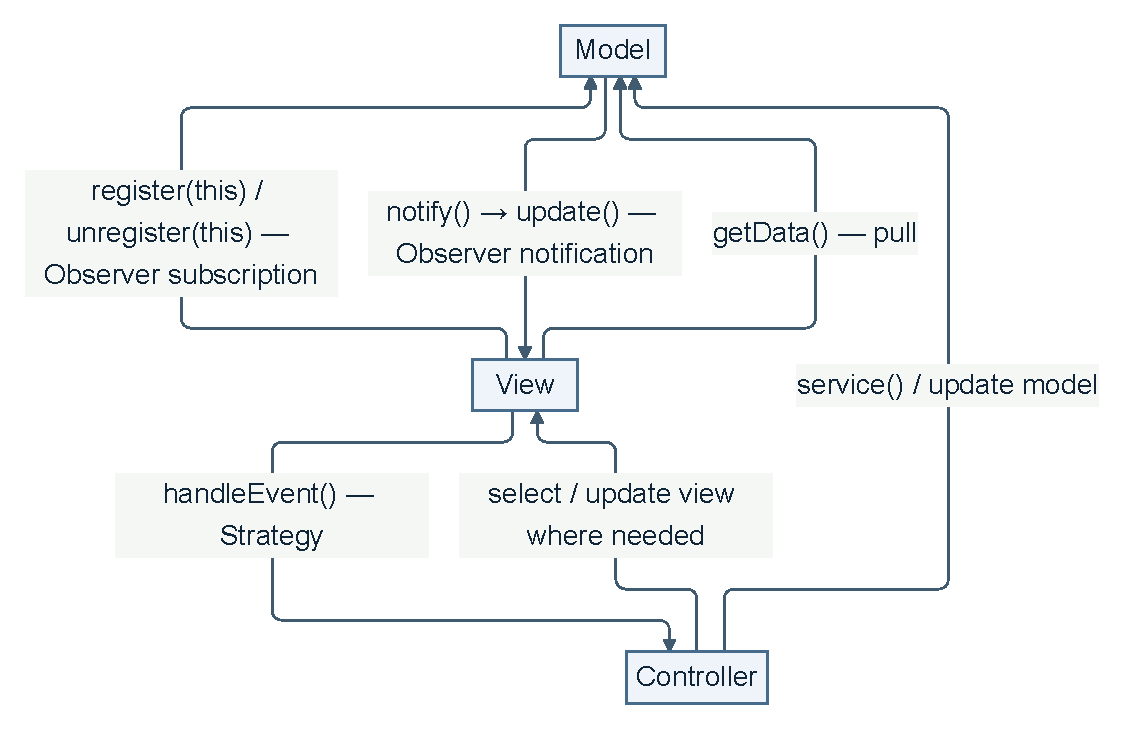
\includegraphics[width=331.20pt]{images/fig-032.pdf}
\captionof{figure}{11.3 The triangular structure (know the arrows by heart)}\end{minipage}\par\smallskip

\textbf{Arrow check:} View registers with Model; Controller invokes Model services; Model notifies subscribed Views; Views pull data and redraw. A subscribed Controller may also receive Model notifications (L15 pp. 22, 25). Observing the Model is different from observing the Controller.

\subsection*{11.4 Which patterns live inside MVC}
\sectionlabel{h-114-which-patterns-live-inside-mvc}

{\fontsize{9}{11}\selectfont
\begin{longtable}{L{\dimexpr 0.34699\linewidth-8.33pt\relax}L{\dimexpr 0.23017\linewidth-5.52pt\relax}L{\dimexpr 0.42284\linewidth-10.15pt\relax}}
\toprule
\rowcolor{ice}\textbf{Relationship} & \textbf{Pattern} & \textbf{Why} \\
\midrule\endfirsthead
\toprule\rowcolor{ice}\textbf{Relationship} & \textbf{Pattern} & \textbf{Why} \\
\midrule\endhead
\multicolumn{3}{r}{\scriptsize Continued on next page}\\\endfoot
\bottomrule\endlastfoot
\textbf{View \ensuremath{\leftrightarrow} Model; subscribed Controller \ensuremath{\leftrightarrow} Model} & \textbf{Observer} & Multiple views, loose coupling, automatic update \\
\textbf{View \ensuremath{\leftrightarrow} Controller} & \textbf{Strategy} & View delegates interface behaviour; controller swappable \ensuremath{\rightarrow} different responses to input; also View \ensuremath{\leftrightarrow} Look \& Feel \\
\textbf{Controller creation /\allowbreak{} Look \& Feel} & \textbf{Abstract Factory} & Create a controller or LAF for a view \\
\textbf{Nested views} & \textbf{Composite} & Panel contains Button; nested Panels \\
\textbf{Extra UI functionality (scrolling)} & \textbf{Decorator} & Attach additional UI functionality to a view \\
\textbf{Undo/\allowbreak{}redo of user actions} & \textbf{Command} & Support undo/\allowbreak{}redo \\
\end{longtable}
}

\begin{studycolumns}
\vspace{0pt}
\subsection*{11.5 Why MVC over plain layering (the exam argument)}
\sectionlabel{h-115-why-mvc-over-plain-layering-the-exam-argument}
\par\needspace{65pt}\phantomsection\label{answer-mvc}
\textbf{Template M --- MVC alternative:} map case state/\allowbreak{}rules to Model, presentations to Views and input handling to Controllers. Use Observer for consistent refresh; Strategy separates input/\allowbreak{}look-and-feel variation; Abstract Factory creates related UI objects. Benefits: multiple-view consistency, separate UI/\allowbreak{}domain change, testability. Costs: notification/\allowbreak{}lifecycle and multi-artifact complexity. It avoids delayed/\allowbreak{}excessive polling and concrete view-to-view callbacks; layering can remain underneath.
\subsection*{11.6 Pros /\allowbreak{} cons}
\sectionlabel{h-116-pros--cons}
\begin{referenceentries}
\textit{\textbf{Pros} / \textbf{Cons}}\par\smallskip
\noindent \textbf{Pros:} \textbf{Simultaneous development} --- multiple views per model; models can have multiple views\par
\noindent \textbf{Cons:} \textbf{Code navigability} and a pronounced \textbf{learning curve}\par\smallskip
\noindent \textbf{Pros:} \textbf{High cohesion} --- related actions grouped on a controller; views for a model grouped\par
\noindent \textbf{Cons:} Framework navigation is complex: new layers of abstraction, users must adapt to MVC's decomposition criteria\par\smallskip
\noindent \textbf{Pros:} \textbf{Low coupling} among models, views and controllers\par
\noindent \textbf{Cons:} \textbf{Multi-artifact consistency} --- one logical change touches three artefacts\par\smallskip
\end{referenceentries}\textbf{Traps:} MVC is not three deployment tiers. Its Controller is not automatically the analysis control stereotype: the course puts View/\allowbreak{}Controller in presentation boundaries, and entities plus business controls in Model. Controller updates Model; Model notifies subscribers; Views pull data and redraw.
\end{studycolumns}

\chapteropen{Chapter 12: Testing fundamentals and basis paths}{chapter-12}
\markboth{Ch. 12 | Testing}{}


\begin{studycolumns}
\vspace{0pt}
\begin{eli5box}
A test is a planned experiment. The input is what you try; the oracle says what should happen; the log records what did happen. Black-box testing asks whether behaviour meets the promise; white-box testing uses the code's branches and paths to choose experiments.
\end{eli5box}
\textbf{Answer check:} State the test level, input and independently justified oracle. For CFG work, keep graph conventions, node/edge counts and feasible traces consistent. CC is a basis size, not a minimum statement/branch suite. Generated tests are not evidence of execution.
\end{studycolumns}

\subsection*{Visual: separate test selection from code coverage}
\sectionlabel{h-visual-separate-test-selection-from-code-coverage}


\par\smallskip\noindent\begin{minipage}{\linewidth}\centering
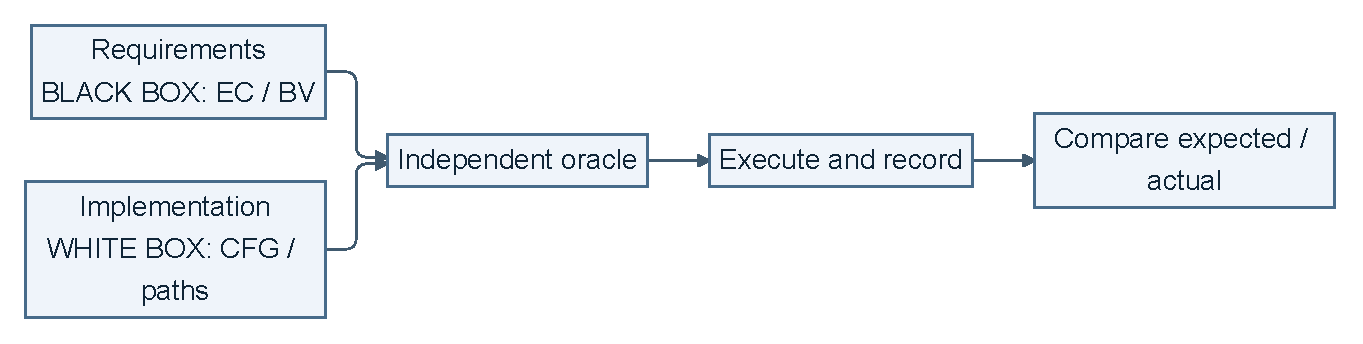
\includegraphics[width=400.66pt]{images/fig-033.pdf}
\captionof{figure}{separate test selection from code coverage}\end{minipage}\par\smallskip

\begin{studycolumns}
\vspace{0pt}



\needspace{4\baselineskip}
\subsection*{12.1 Definitions}
\sectionlabel{h-121-definitions}

\begin{quote}\small\color{navy}
A \textbf{software bug} is \emph{an error, flaw, failure or fault in a computer program or system that causes it to produce an incorrect or unexpected result, or to behave in unintended ways.}

\end{quote}


\begin{quote}\small\color{navy}
\textbf{Software testing} is \emph{an investigation conducted to provide stakeholders with information about the quality of the software product or service under test.}

\end{quote}
Three properties that decide many MCQs:

\begin{enumerate}
\item It is \textbf{dynamic execution} (you run the software).
\item It aims \textbf{to find bugs, not to prove that no bugs exist} (Dijkstra).
\item It reduces the \textbf{perceived risk} of the system not working to an acceptable value.
\end{enumerate}
\textbf{Not testing:} testing \ensuremath{\neq} debugging. Testing finds the failure; debugging locates and fixes the fault.

\needspace{4\baselineskip}
\subsection*{12.2 Why exhaustive testing is impossible}
\sectionlabel{h-122-why-exhaustive-testing-is-impossible}
For a 16-bit integer there are \textbf{2\textsuperscript{1}\textsuperscript{6} = 65 536} inputs. Even that is affordable once, but for realistic signatures the input space is astronomically large, so we must \textbf{select} inputs cleverly. That selection is exactly what \textbf{EC} and \textbf{BV} testing formalise.

\textbf{Selection rule:} random samples can miss the small regions where a defect changes output; use EC/BV to target those regions.
\end{studycolumns}

\Needspace{4\baselineskip}
\subsection*{12.3 Black box vs white box}
\sectionlabel{h-123-black-box-vs-white-box}


{\fontsize{9}{11}\selectfont
\begin{longtable}{L{\dimexpr 0.19829\linewidth-4.76pt\relax}L{\dimexpr 0.46795\linewidth-11.23pt\relax}L{\dimexpr 0.33377\linewidth-8.01pt\relax}}
\toprule
\rowcolor{ice}\textbf{} & \textbf{\textbf{Black box}} & \textbf{\textbf{White box}} \\
\midrule\endfirsthead
\toprule\rowcolor{ice}\textbf{} & \textbf{\textbf{Black box}} & \textbf{\textbf{White box}} \\
\midrule\endhead
\multicolumn{3}{r}{\scriptsize Continued on next page}\\\endfoot
\bottomrule\endlastfoot
What to analyse & \textbf{Requirements and specifications} & \textbf{Implementation details}, internal paths and structure \\
Example requirement & "The income of an applicant must be between \$1500 and \$8000 per month" & --- \\
Techniques & \textbf{Equivalence class testing, boundary value testing}, state-based testing & \textbf{Control flow testing} (CFG, basis paths), data flow testing \\
Pros & Directs the tester to a \textbf{very small subset} of inputs likely to find bugs; applicable at \textbf{all levels} & Gives a \textbf{coverage} notion \\
Cons & \textbf{Cannot infer code coverage from black-box inputs alone}; EC/\allowbreak{}requirement coverage can still be tracked & Needs code; misses "missing requirement" bugs \\
\end{longtable}
}

\begin{studycolumns}
\vspace{0pt}

\needspace{4\baselineskip}
\subsection*{12.4 Levels of testing (4)}
\sectionlabel{h-124-levels-of-testing-4}

\begin{referenceentries}
\textit{\textbf{Level} / \textbf{Scope}}\par\smallskip
\noindent \textbf{\textbf{Unit testing}}: Test a unit individually (the level used in this course)\par
\noindent \textbf{\textbf{Integration testing}}: Test units \textbf{in combination}\par
\noindent \textbf{\textbf{System testing}}: Everything: functionality, usability, reliability, performance, portability, security\ldots{}\par
\noindent \textbf{\textbf{Acceptance testing (UAT)}}: Customer accepts the software and pays\par
\end{referenceentries}
\needspace{4\baselineskip}
\subsection*{12.5 Ingredients of a test case (5 --- memorise)}
\sectionlabel{h-125-ingredients-of-a-test-case-5--memorise}

\begin{referenceentries}
\textit{\textbf{Ingredient} / \textbf{Description}}\par\smallskip
\noindent \textbf{\textbf{Name}}: Distinct name of the test case\par
\noindent \textbf{\textbf{Location}}: Path to the test program and its inputs\par
\noindent \textbf{\textbf{Input}}: Input data or commands\par
\noindent \textbf{\textbf{Oracle}}: \textbf{Expected} test output\par
\noindent \textbf{\textbf{Log}}: \textbf{Actual} output produced by the test\par
\end{referenceentries}
JUnit mapping: \code{@Test public void test\allowbreak{}Qualified\allowbreak{}Application()} = \textbf{Name}; the class/\allowbreak{}package = \textbf{Location}; the arguments to \code{analyze\allowbreak{}Application(.\allowbreak{}.\allowbreak{}.\allowbreak{})} = \textbf{Input}; the expected argument in \code{assert\allowbreak{}Equals(Application\allowbreak{}Result.\allowbreak{}Approval,\allowbreak{} result)} = \textbf{Oracle}; the recorded actual \code{result} and test report = \textbf{Log}.


\begin{quote}\small\color{navy}
\textbf{Trap:} \emph{oracle} = expected; \emph{log} = actual. Keep this distinction when naming test-case components.

\textbf{Oracle check:} derive expected behaviour from requirements; separately validate wrong requirements with stakeholders.

\end{quote}
\end{studycolumns}

\Needspace{4\baselineskip}
\subsection*{12.6 Execution order: cascading vs independent tests}
\sectionlabel{h-126-execution-order-cascading-vs-independent-tests}


{\fontsize{9}{11}\selectfont
\begin{longtable}{L{\dimexpr 0.20210\linewidth-4.85pt\relax}L{\dimexpr 0.41868\linewidth-10.05pt\relax}L{\dimexpr 0.37922\linewidth-9.10pt\relax}}
\toprule
\rowcolor{ice}\textbf{} & \textbf{\textbf{Cascading (dependent)}} & \textbf{\textbf{Independent}} \\
\midrule\endfirsthead
\toprule\rowcolor{ice}\textbf{} & \textbf{\textbf{Cascading (dependent)}} & \textbf{\textbf{Independent}} \\
\midrule\endhead
\multicolumn{3}{r}{\scriptsize Continued on next page}\\\endfoot
\bottomrule\endlastfoot
Shape & Create \ensuremath{\rightarrow} Read \ensuremath{\rightarrow} Update \ensuremath{\rightarrow} Delete \ensuremath{\rightarrow} Read-deleted (each builds on the last) & Self-contained cases for each feature \\
YES Benefit & \textbf{Smaller and simpler} test cases; realistic end-to-end sequence & \textbf{Parallel} test execution; failures are isolated \\
NO Cost & \textbf{One failure invalidates subsequent tests} & \textbf{Larger and more complex} test cases (each sets up its own state) \\
\end{longtable}
}

\begin{studycolumns}
\vspace{0pt}

\needspace{4\baselineskip}
\subsection*{12.7 Basis path testing (white box)}
\sectionlabel{h-127-basis-path-testing-white-box}

\begin{quote}\small\color{navy}
\textbf{Basis path testing} (structured testing) is a white-box method for designing test cases intended to exercise a \textbf{basis set of linearly independent control-flow paths}.

\end{quote}
Process:

\begin{enumerate}
\item Draw the \textbf{Control Flow Graph (CFG)}.
\item Compute the \textbf{Cyclomatic Complexity (CC)}.
\item Derive a set of \textbf{linearly independent paths} (the basis set) --- there are \textbf{CC} of them.
\item Generate a test case for \textbf{each} basis path.
\end{enumerate}
\textbf{Cyclomatic complexity (three equivalent formulas):}


\begin{ReferenceCode}
CC = E - N + 2        (E = edges, N = nodes; per connected component, P components -> +2P)
CC = number of binary decision nodes + 1   (one connected CFG)
CC = number of bounded regions + 1
\end{ReferenceCode}
For a connected, single-entry/\allowbreak{}single-exit CFG, CC is the number of paths in a \textbf{graph basis}. It is \textbf{not} a minimum for statement or branch coverage. Some graph paths are infeasible because of program data, so a structural basis is not automatically an executable test suite. L16, p. 10, loosely says ``all possible paths''; p. 11 illustrates a basis set instead. Loops can create infinitely many execution paths, so these are different coverage goals.

\textbf{Worked CFG:} Section 12.9 distinguishes graph bases from feasible execution and minimum coverage suites.
\end{studycolumns}

\Needspace{4\baselineskip}
\subsection*{12.8 Coverage criteria}
\sectionlabel{h-128-coverage-criteria}


{\fontsize{9}{11}\selectfont
\begin{longtable}{L{\dimexpr 0.26822\linewidth-6.44pt\relax}L{\dimexpr 0.39315\linewidth-9.44pt\relax}L{\dimexpr 0.33864\linewidth-8.13pt\relax}}
\toprule
\rowcolor{ice}\textbf{Criterion} & \textbf{Requirement} & \textbf{Implication} \\
\midrule\endfirsthead
\toprule\rowcolor{ice}\textbf{Criterion} & \textbf{Requirement} & \textbf{Implication} \\
\midrule\endhead
\multicolumn{3}{r}{\scriptsize Continued on next page}\\\endfoot
\bottomrule\endlastfoot
\textbf{Statement coverage} & Every \textbf{node} executed at least once & Weakest; misses branch-only bugs \\
\textbf{Branch (decision) coverage} & Every \textbf{edge} (true and false of every decision) taken at least once & \textbf{100\% branch \ensuremath{\Rightarrow} 100\% statement}, but not vice versa \\
\textbf{Path coverage} & Every \textbf{path} executed & Usually infeasible (loops \ensuremath{\Rightarrow} infinite paths) \\
\textbf{Basis-path coverage} & A feasible independent path set exercised; report infeasible structural paths & Practical middle ground \\
\end{longtable}
}

\begin{studycolumns}
\vspace{0pt}


\begin{quote}\small\color{navy}
\textbf{Trap:} "statement coverage implies branch coverage" is \textbf{false} (a \code{if} with no \code{else} whose body always executes gives 100\% statement but not 100\% branch). The reverse \emph{is} true.

\end{quote}
\needspace{4\baselineskip}
\subsection*{12.9 Worked white-box example you should be able to reproduce --- Tutorial 9}
\sectionlabel{h-129-worked-white-box-example-you-should-be-able-to-reproduce--tutorial-9}

\begin{ReferenceCode}
public int sum(int n, int upperbound){
 1  int result, i;
 2  result = 0;
 3  i = 0;
 4  if(n < 0) {
 5    n = -n;
 6  }
 7  while(i<n && result <= upperbound){
 8    i = i + 1;
 9    result = result + i;
10  }
11  if(result <= upperbound){
12    System.out.println("The sum is " + result);
13  } else {
14    System.out.println("The sum is too large!");
15  }
16  return result;
}
\end{ReferenceCode}
\textbf{CFG} --- 12 nodes (1, 2, 3, 4, 5, 7, 8, 9, 11, 12, 14, 16); the compound \code{while} guard is \textbf{one} node:


\needspace{273pt}
\par\smallskip\noindent\begin{minipage}{\linewidth}\centering
\begin{minipage}[t]{0.488\linewidth}\centering\scriptsize\textbf{1}\par\smallskip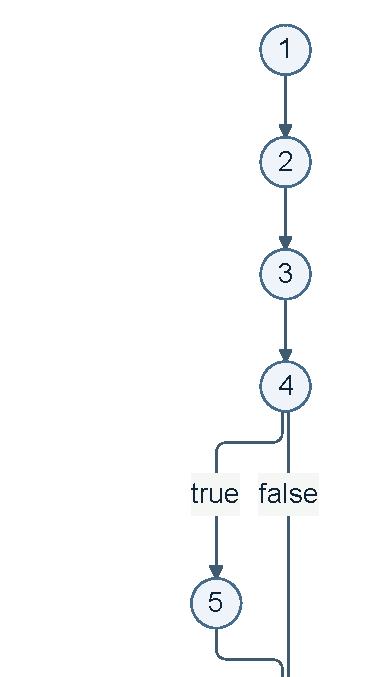
\includegraphics[width=108.10pt]{images/fig-035-compact-1.pdf}\end{minipage}\hfill
\begin{minipage}[t]{0.488\linewidth}\centering\scriptsize\textbf{2}\par\smallskip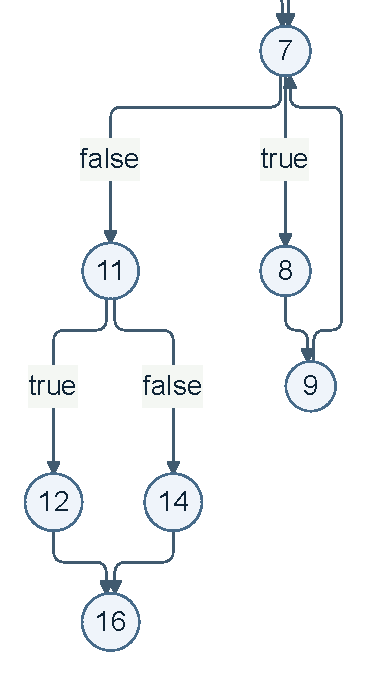
\includegraphics[width=108.10pt]{images/fig-035-compact-2.pdf}\end{minipage}
\captionof{figure}{12.9 Worked white-box example you should be able to reproduce --- Tutorial 9 --- follow numbered panels; crossing arrows continue.}\end{minipage}\par\smallskip


Exact edge list: \code{1\ensuremath{\rightarrow}2,\allowbreak{} 2\ensuremath{\rightarrow}3,\allowbreak{} 3\ensuremath{\rightarrow}4,\allowbreak{} 4\ensuremath{\rightarrow}5,\allowbreak{} 4\ensuremath{\rightarrow}7,\allowbreak{} 5\ensuremath{\rightarrow}7,\allowbreak{} 7\ensuremath{\rightarrow}8,\allowbreak{} 7\ensuremath{\rightarrow}11,\allowbreak{} 8\ensuremath{\rightarrow}9,\allowbreak{} 9\ensuremath{\rightarrow}7,\allowbreak{} 11\ensuremath{\rightarrow}12,\allowbreak{} 11\ensuremath{\rightarrow}14,\allowbreak{} 12\ensuremath{\rightarrow}16,\allowbreak{} 14\ensuremath{\rightarrow}16}.

\textbf{N = 12, E = 14 \ensuremath{\Rightarrow} CC = E \ensuremath{-} N + 2 = 14 \ensuremath{-} 12 + 2 = 4.} \emph{(Cross-check by predicates: \code{if(n<0)}, the \code{while}, \code{if(result <=\allowbreak{} upperbound)} = 3 decisions \ensuremath{\Rightarrow} 3 + 1 = 4.)}

\textbf{One feasible basis set for the combined-guard CFG (CC = 4):}
\end{studycolumns}


{\fontsize{9}{11}\selectfont
\begin{longtable}{L{\dimexpr 0.09590\linewidth-3.07pt\relax}L{\dimexpr 0.28882\linewidth-9.24pt\relax}L{\dimexpr 0.25186\linewidth-8.06pt\relax}L{\dimexpr 0.36342\linewidth-11.63pt\relax}}
\toprule
\rowcolor{ice}\textbf{\#} & \textbf{Path} & \textbf{Covering input} & \textbf{Expected output} \\
\midrule\endfirsthead
\toprule\rowcolor{ice}\textbf{\#} & \textbf{Path} & \textbf{Covering input} & \textbf{Expected output} \\
\midrule\endhead
\multicolumn{4}{r}{\scriptsize Continued on next page}\\\endfoot
\bottomrule\endlastfoot
1 & 1,2,3,4,7,11,12,16 & n = 0, ub = 100 & prints "The sum is 0", returns 0 \\
2 & 1,2,3,4,7,8,9,7,11,12,16 & n = 1, ub = 100 & prints "The sum is 1", returns 1 \\
3 & 1,2,3,4,5,7,8,9,7,11,12,16 & n = \ensuremath{-}1, ub = 100 & prints "The sum is 1", returns 1 \\
4 & 1,2,3,4,7,8,9,7,11,14,16 & n = 1, ub = 0 & prints "The sum is too large!", returns 1 \\
\end{longtable}
}

\textbf{Statement and branch coverage need only two tests}, not four:




{\fontsize{9}{11}\selectfont
\begin{longtable}{L{\dimexpr 0.30144\linewidth-7.23pt\relax}L{\dimexpr 0.35048\linewidth-8.41pt\relax}L{\dimexpr 0.34807\linewidth-8.35pt\relax}}
\toprule
\rowcolor{ice}\textbf{Input} & \textbf{Executed path} & \textbf{Expected print /\allowbreak{} return} \\
\midrule\endfirsthead
\toprule\rowcolor{ice}\textbf{Input} & \textbf{Executed path} & \textbf{Expected print /\allowbreak{} return} \\
\midrule\endhead
\multicolumn{3}{r}{\scriptsize Continued on next page}\\\endfoot
\bottomrule\endlastfoot
\code{n =\allowbreak{} \ensuremath{-}1,\allowbreak{} upperbound =\allowbreak{} 100} & \code{1,\allowbreak{}2,\allowbreak{}3,\allowbreak{}4,\allowbreak{}5,\allowbreak{}7,\allowbreak{}8,\allowbreak{}9,\allowbreak{}7,\allowbreak{}11,\allowbreak{}12,\allowbreak{}16} & \code{The sum is 1} /\allowbreak{} \code{1} \\
\code{n =\allowbreak{} 5,\allowbreak{} upperbound =\allowbreak{} 1} & \code{1,\allowbreak{}2,\allowbreak{}3,\allowbreak{}4,\allowbreak{}7,\allowbreak{}8,\allowbreak{}9,\allowbreak{}7,\allowbreak{}8,\allowbreak{}9,\allowbreak{}7,\allowbreak{}11,\allowbreak{}14,\allowbreak{}16} & \code{The sum is too large!} /\allowbreak{} \code{3} \\
\end{longtable}
}

\begin{studycolumns}
\vspace{0pt}

Together these cover all executable statements and both outcomes of each of the three combined decisions. Two is minimal because the final \code{if} takes only one outcome per call. Four paths are needed for the \textbf{illustrated basis set}, a stronger, different target. The method returns the sum \textbf{after} it has crossed the bound; it does not clamp the return value to \code{upperbound}.

\textbf{Compound-condition convention:} treating the whole \code{while} guard as node 7 gives \textbf{N = 12, E = 14, CC = 4}. Splitting short-circuit \code{\&\&} into nodes 7a (\code{i<n}) and 7b (\code{result<=\allowbreak{}upperbound}) gives \textbf{N = 13, E = 16, CC = 5}. In the split graph, 7a false skips 7b; 7a true reaches 7b; either false exits to 11. State the convention and make the formula match the graph.

The same two coverage tests above also exercise both outcomes of both operands in the split graph: the first ends with \code{i<n} false; the second ends with \code{i<n} true and \code{result<=\allowbreak{}upperbound} false. If a fifth basis path is requested for that graph, add \code{n =\allowbreak{} 1,\allowbreak{} upperbound =\allowbreak{} \ensuremath{-}1}: it skips the body because 7b is false immediately, prints \code{The sum is too large!} and returns \code{0}.

\textbf{Trace carefully:} \code{n =\allowbreak{} 4} with a large bound executes four iterations. A single iteration can be obtained with \code{n =\allowbreak{} 1} and a non-negative bound; \code{n =\allowbreak{} 2} needs a bound that stops the loop after the first addition. A claimed basis path must either match its stated input exactly or be labelled schematic.
\end{studycolumns}

\chapteropen{Chapter 13: Equivalence classes and boundary values}{chapter-13}
\markboth{Ch. 13 | EC and BV}{}


\begin{studycolumns}
\vspace{0pt}
\begin{eli5box}
Instead of trying every possible age, sort inputs into buckets that should behave alike. Then test the fence edges: just below, exactly on and just above. If you test two broken fields together, the first error may hide the second, so defensive tests usually break one parameter at a time.
\end{eli5box}
\textbf{Answer check:} State units, representation and inclusive endpoints; partition valid/invalid behaviour, then select full boundary triplets. Combine valid inputs and isolate one invalid parameter per defensive row. Give an oracle. String length, syntax, registration and dependency failures are separate checks.
\end{studycolumns}

\subsection*{Visual: build tests in the right order}
\sectionlabel{h-visual-build-tests-in-the-right-order}


\par\smallskip\noindent\begin{minipage}{\linewidth}\centering
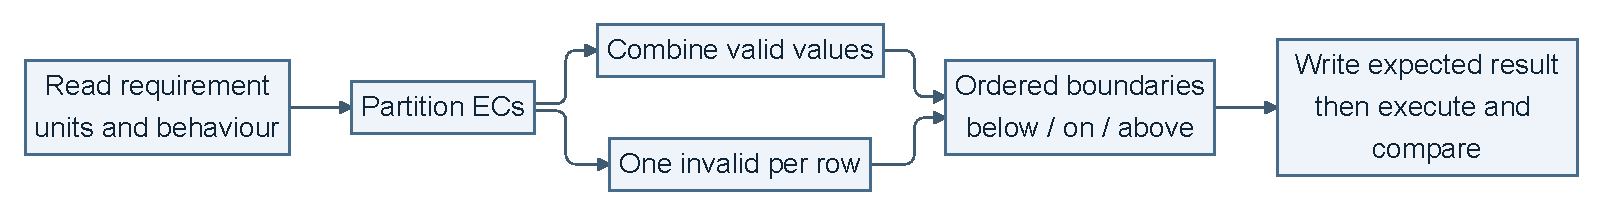
\includegraphics[width=471.96pt]{images/fig-036.pdf}
\captionof{figure}{build tests in the right order}\end{minipage}\par\smallskip

\begin{studycolumns}
\vspace{0pt}



\needspace{4\baselineskip}
\subsection*{13.1 Two assumptions behind black-box testing}
\sectionlabel{h-131-two-assumptions-behind-black-box-testing}
\begin{enumerate}
\item \textbf{A verifiable requirement /\allowbreak{} API specification exists} --- make software testable from inception. \emph{Not verifiable:} "The company must not hire too-young or too-old people." \emph{Verifiable:} "0--15 and 55--99: do not hire; 16--17: part-time; 18--54: full-time."
\item \textbf{The code must be testable} --- a 100-branch \code{if (age=\allowbreak{}=\allowbreak{}0) \ldots{} if (age=\allowbreak{}=\allowbreak{}99)} chain makes black-box testing ineffective compared with range conditions.
\end{enumerate}
\needspace{4\baselineskip}
\subsection*{13.2 Equivalence classes}
\sectionlabel{h-132-equivalence-classes}

\begin{quote}\small\color{navy}
A set of input values forms an \textbf{equivalence class (EC)} if:

\begin{itemize}
\item they are all \textbf{supposed to produce the same output};
\item if one value catches a bug, the others \textbf{probably will too};
\item if one value does not catch a bug, the others \textbf{probably will not either}.
\end{itemize}
\end{quote}
\end{studycolumns}

\Needspace{4\baselineskip}
\subsection*{13.3 Partition rules}
\sectionlabel{h-133-partition-rules}


{\fontsize{9}{11}\selectfont
\begin{longtable}{L{\dimexpr 0.34307\linewidth-8.23pt\relax}L{\dimexpr 0.36021\linewidth-8.64pt\relax}L{\dimexpr 0.29672\linewidth-7.12pt\relax}}
\toprule
\rowcolor{ice}\textbf{Input type} & \textbf{Valid ECs} & \textbf{Invalid ECs} \\
\midrule\endfirsthead
\toprule\rowcolor{ice}\textbf{Input type} & \textbf{Valid ECs} & \textbf{Invalid ECs} \\
\midrule\endhead
\multicolumn{3}{r}{\scriptsize Continued on next page}\\\endfoot
\bottomrule\endlastfoot
\textbf{Range of values} (\code{1500 \ensuremath{\leq} x \ensuremath{\leq} 80000}) & \textbf{ONE} valid EC (or more, if the requirement has several valid ranges --- e.g. hiring rules have 4) & \textbf{TWO} invalid ECs (\code{x \ensuremath{\leq} 1499} and \code{x \ensuremath{\geq} 80001}) \\
\textbf{Discrete values} (applicant type \ensuremath{\in} \{Person\}, property type \ensuremath{\in} \{HDB, Condo\}) & \textbf{ONE} valid EC (the listed set) & \textbf{ONE} invalid EC (everything else) \\
\end{longtable}
}

Worked partitions:




{\fontsize{9}{11}\selectfont
\begin{longtable}{L{\dimexpr 0.34550\linewidth-8.29pt\relax}L{\dimexpr 0.31302\linewidth-7.51pt\relax}L{\dimexpr 0.34148\linewidth-8.20pt\relax}}
\toprule
\rowcolor{ice}\textbf{Parameter} & \textbf{Valid EC(s)} & \textbf{Invalid EC(s)} \\
\midrule\endfirsthead
\toprule\rowcolor{ice}\textbf{Parameter} & \textbf{Valid EC(s)} & \textbf{Invalid EC(s)} \\
\midrule\endhead
\multicolumn{3}{r}{\scriptsize Continued on next page}\\\endfoot
\bottomrule\endlastfoot
Mortgage income (1500--80000) & 1500 \ensuremath{\leq} x \ensuremath{\leq} 80000 & x \ensuremath{\leq} 1499 ; x \ensuremath{\geq} 80001 \\
\#mortgages (0--5) & 0 \ensuremath{\leq} x \ensuremath{\leq} 5 & x \ensuremath{\leq} \ensuremath{-}1 ; x \ensuremath{\geq} 6 \\
Password length (4--8) & 4 \ensuremath{\leq} x \ensuremath{\leq} 8 & x \ensuremath{\leq} 3 ; x \ensuremath{\geq} 9 \\
Password characters (a--z, A--Z, 0--9) & \{a\ldots{}z, A\ldots{}Z, 0\ldots{}9\} & everything else (+, \ensuremath{-}, (, ), \ldots{}) \\
Applicant type (Person only) & \{Person\} & \{Company, Trust, Partnership, \ldots{}\} \\
Property type (HDB, Condo) & \{HDB, Condo\} & \{Townhouse, MobileHome, \ldots{}\} \\
Hiring age & 0--15 (no hire) ; 16--17 (part) ; 18--54 (full) ; 55--99 (no hire) & age \ensuremath{\leq} \ensuremath{-}1 ; age \ensuremath{\geq} 100 \\
\end{longtable}
}

\begin{studycolumns}
\vspace{0pt}


\begin{quote}\small\color{navy}
\textbf{Trap:} counting the \emph{hiring} rule as "one valid EC" is wrong --- there are \textbf{four} valid ECs because the lecture partitions \textbf{four contiguous ranges}. The two ``no hire'' ranges share an output but have different boundaries; four ranges do not mean four distinct output values.

\end{quote}
\needspace{4\baselineskip}
\subsection*{13.4 Designing test cases from ECs --- the two golden rules}
\sectionlabel{h-134-designing-test-cases-from-ecs--the-two-golden-rules}
\begin{enumerate}
\item \textbf{Valid tests:} you \textbf{may combine} valid values of \textbf{several} parameters in one test case --- choose one value from one EC of each parameter.
\item \textbf{Invalid tests:} \textbf{exactly ONE invalid value} per test case (one parameter, one EC); all other parameters take \textbf{valid} values.
\end{enumerate}
\textbf{Why only one invalid per case?} So that the failure can be attributed: you learn the error handling and behaviour for \textbf{each type of invalid input}. With four invalid values in one row, a rejection tells you nothing about which input caused it --- and error handling may mask each other.

\textbf{Small ECs:} testing every member can be practical for small sets/ranges, but does not make each member a separate EC.

\textbf{Testing by contract vs defensive testing}
\end{studycolumns}


{\fontsize{9}{11}\selectfont
\begin{longtable}{L{\dimexpr 0.22243\linewidth-5.34pt\relax}L{\dimexpr 0.32582\linewidth-7.82pt\relax}L{\dimexpr 0.45175\linewidth-10.84pt\relax}}
\toprule
\rowcolor{ice}\textbf{} & \textbf{\textbf{Testing by contract}} & \textbf{\textbf{Defensive testing}} \\
\midrule\endfirsthead
\toprule\rowcolor{ice}\textbf{} & \textbf{\textbf{Testing by contract}} & \textbf{\textbf{Defensive testing}} \\
\midrule\endhead
\multicolumn{3}{r}{\scriptsize Continued on next page}\\\endfoot
\bottomrule\endlastfoot
Cases & \textbf{Only valid} inputs (satisfying pre-conditions) & \textbf{Both valid and invalid} inputs \\
Assumption & Users use the code as intended & Users will not; test that invalid input does not cause unforeseen errors or abnormal termination \\
Preferred by & --- & \textbf{Testers} (if it breaks, the tester is blamed) \\
\end{longtable}
}

\Needspace{4\baselineskip}
\subsection*{13.5 Boundary value testing (BVT)}
\sectionlabel{h-135-boundary-value-testing-bvt}

\subsubsection*{Visual: see the mortgage-income partitions and their edges}
\sectionlabel{h-visual-see-the-mortgage-income-partitions-and-their-edges}



\par\smallskip\noindent\begin{minipage}{\linewidth}\centering
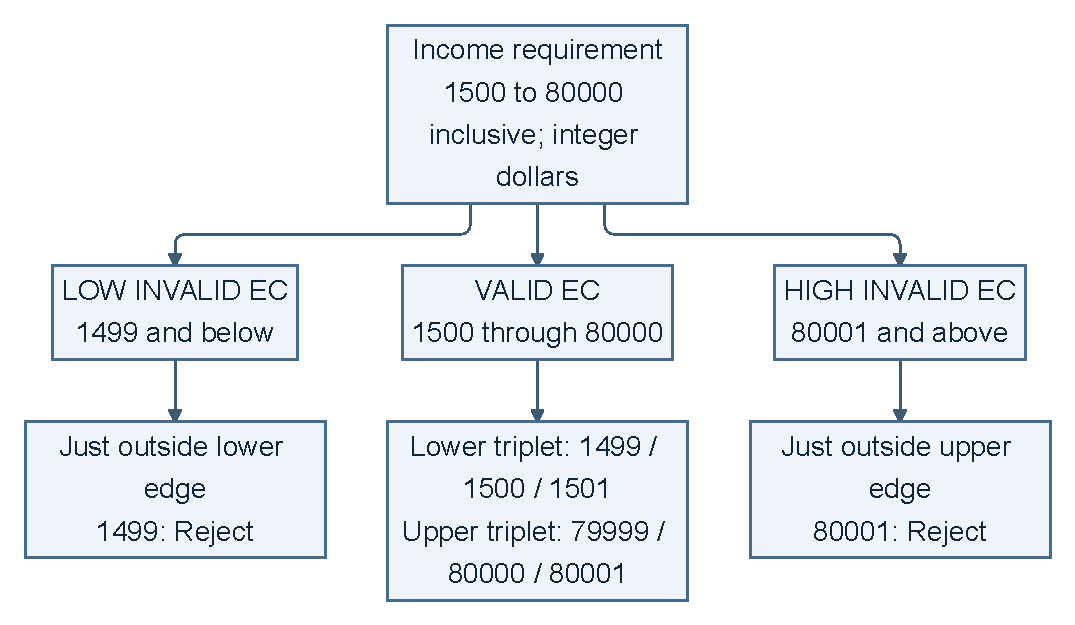
\includegraphics[width=316.48pt]{images/fig-037.pdf}
\captionof{figure}{see the mortgage-income partitions and their edges}\end{minipage}\par\smallskip

\begin{studycolumns}
\vspace{0pt}



\begin{quote}\small\color{navy}
For \textbf{each boundary of each range-of-values EC}, choose \textbf{three} values: one \textbf{on-the-boundary}, one \textbf{just-below}, one \textbf{just-above}. The size of the "just" step depends on the \textbf{unit} of the value.

\end{quote}
\textbf{In the lecture's terminology}, range-of-values parameters include integer counts. ``Discrete values'' means \textbf{unordered categories} such as Person/\allowbreak{}Company and HDB/\allowbreak{}Condo, which have no numeric BVs. Integer quantities such as mortgage count \textbf{do} have BVs.

\textbf{Worked BVs (full triplets, with the lecture's reduced valid/\allowbreak{}invalid selection):}
\end{studycolumns}


{\fontsize{9}{11}\selectfont
\begin{longtable}{L{\dimexpr 0.21399\linewidth-8.56pt\relax}L{\dimexpr 0.20246\linewidth-8.10pt\relax}L{\dimexpr 0.20697\linewidth-8.28pt\relax}L{\dimexpr 0.18829\linewidth-7.53pt\relax}L{\dimexpr 0.18829\linewidth-7.53pt\relax}}
\toprule
\rowcolor{ice}\textbf{Requirement} & \textbf{Lower boundary} & \textbf{Upper boundary} & \textbf{Valid BVs} & \textbf{Invalid BVs} \\
\midrule\endfirsthead
\toprule\rowcolor{ice}\textbf{Requirement} & \textbf{Lower boundary} & \textbf{Upper boundary} & \textbf{Valid BVs} & \textbf{Invalid BVs} \\
\midrule\endhead
\multicolumn{5}{r}{\scriptsize Continued on next page}\\\endfoot
\bottomrule\endlastfoot
Income 1500--80000 & 1499, \textbf{1500}, 1501 & 79999, \textbf{80000}, 80001 & \{1500, 80000\} & \{1499, 80001\} \\
\#mortgages 0--5 & \textbf{\ensuremath{-}1}, 0, 1 & 4, \textbf{5}, 6 & \{0, 5\} & \{\ensuremath{-}1, 6\} \\
Password length 4--8 & 3, \textbf{4}, 5 & 7, \textbf{8}, 9 & \{4, 8\} & \{3, 9\} \\
Hiring age 0--15 & \ensuremath{-}1, \textbf{0}, 1 & 14, \textbf{15}, 16 & \{0, 15\} (see de-dup below) & \{\ensuremath{-}1, 100\} \\
Hiring age 16--17 & 15, \textbf{16}, 17 & 16, \textbf{17}, 18 & \ldots{} & \ldots{} \\
Hiring age 18--54 & 17, \textbf{18}, 19 & 53, \textbf{54}, 55 & \ldots{} & \ldots{} \\
Hiring age 55--99 & 54, \textbf{55}, 56 & 98, \textbf{99}, 100 & \ldots{} & \ldots{} \\
\end{longtable}
}

\begin{studycolumns}
\vspace{0pt}

Following the \textbf{course's reduced BV selection}, the hiring sets are: \textbf{valid BVs = \{0, 15, 16, 17, 18, 54, 55, 99\}}; \textbf{invalid BVs = \{\ensuremath{-}1, 100\}}.

\textbf{The course's test-reduction rule (L18, pp. 11--15):}


\begin{quote}\small\color{navy}
Remove the just-below /\allowbreak{} just-above value from an EC's BVs (do \textbf{not} create a duplicate test case) if that value \textbf{falls into another EC} --- including the \emph{current} EC.

\end{quote}
Concretely: a just-below/\allowbreak{}just-above value is used as an \textbf{invalid test value only if it lies outside all valid ECs}. If it lands in another valid EC, that EC's own on-the-boundary value already covers it. (For 0--15, 1 is omitted because it stays inside the same EC; 16 is already a boundary of the next EC.) This is \textbf{more than removing equal duplicate values}: the slides also omit distinct interior neighbours. State the full triplets when asked for BVs, then identify the reduced test selection. Keeping all distinct triplet values is a valid stronger test suite; do not claim those values are duplicates.

\needspace{4\baselineskip}
\subsection*{13.6 Designing test cases from BVs}
\sectionlabel{h-136-designing-test-cases-from-bvs}
Same two rules as ECs, with BVs supplying the values:

\begin{itemize}
\item \textbf{Valid test cases:} combination of \textbf{on-the-boundary (valid) values}, one from each EC, combined across parameters.
\item \textbf{Invalid test cases:} \textbf{one} just-below/\allowbreak{}just-above (invalid) value per test case, with valid values for all other parameters.
\end{itemize}
For two range parameters \emph{A} and \emph{B}, the lecture uses these three test shapes:

\begin{enumerate}
\item \textbf{Valid A + Valid B} \ensuremath{\rightarrow} combination of valid inputs.
\item \textbf{Valid A + Invalid B} \ensuremath{\rightarrow} one invalid.
\item \textbf{Invalid A + Valid B} \ensuremath{\rightarrow} one invalid.
\end{enumerate}
\needspace{4\baselineskip}
\subsection*{13.7 Worked full example --- Mortgage application}
\sectionlabel{h-137-worked-full-example--mortgage-application}
\textbf{Requirements}

\begin{itemize}
\item Income must be \textbf{\$1500--\$80000/\allowbreak{}month} (L17/\allowbreak{}L18 worked problem, not L16's separate \$8000 example).
\item Number of mortgages per applicant must be \textbf{0--5}.
\item Only \textbf{Person} applicants are approved.
\item Only \textbf{HDB} and \textbf{Condo} properties are approved.
\end{itemize}
\textbf{ECs}
\end{studycolumns}


{\fontsize{9}{11}\selectfont
\begin{longtable}{L{\dimexpr 0.21333\linewidth-6.83pt\relax}L{\dimexpr 0.21333\linewidth-6.83pt\relax}L{\dimexpr 0.24633\linewidth-7.88pt\relax}L{\dimexpr 0.32702\linewidth-10.46pt\relax}}
\toprule
\rowcolor{ice}\textbf{Parameter} & \textbf{Valid EC(s)} & \textbf{Invalid EC(s)} & \textbf{BVs} \\
\midrule\endfirsthead
\toprule\rowcolor{ice}\textbf{Parameter} & \textbf{Valid EC(s)} & \textbf{Invalid EC(s)} & \textbf{BVs} \\
\midrule\endhead
\multicolumn{4}{r}{\scriptsize Continued on next page}\\\endfoot
\bottomrule\endlastfoot
Income & 1500--80000 & \ensuremath{\leq}1499 ; \ensuremath{\geq}80001 & valid \{1500, 80000\}; invalid \{1499, 80001\} \\
\#mortgage & 0--5 & \ensuremath{\leq}\ensuremath{-}1 ; \ensuremath{\geq}6 & valid \{0, 5\}; invalid \{\ensuremath{-}1, 6\} (you may additionally enumerate 1--4) \\
Applicant type & \{Person\} & \{Company, Trust, \ldots{}\} & none (discrete) \\
Property type & \{HDB, Condo\} & \{Townhouse, MobileHome, \ldots{}\} & none (discrete) \\
\end{longtable}
}

\textbf{Valid test cases} (combining valid values; enumerating the small discrete/\allowbreak{}range ECs)




{\fontsize{9}{11}\selectfont
\begin{longtable}{L{\dimexpr 0.07749\linewidth-3.72pt\relax}L{\dimexpr 0.18450\linewidth-8.86pt\relax}L{\dimexpr 0.18450\linewidth-8.86pt\relax}L{\dimexpr 0.18450\linewidth-8.86pt\relax}L{\dimexpr 0.18450\linewidth-8.86pt\relax}L{\dimexpr 0.18450\linewidth-8.86pt\relax}}
\toprule
\rowcolor{ice}\textbf{\#} & \textbf{Income} & \textbf{\#mortgage} & \textbf{Applicant} & \textbf{Property} & \textbf{Expected} \\
\midrule\endfirsthead
\toprule\rowcolor{ice}\textbf{\#} & \textbf{Income} & \textbf{\#mortgage} & \textbf{Applicant} & \textbf{Property} & \textbf{Expected} \\
\midrule\endhead
\multicolumn{6}{r}{\scriptsize Continued on next page}\\\endfoot
\bottomrule\endlastfoot
1 & \$1500 & 0 & Person & Condo & Approval \\
2 & \$2000 & 1 & Person & Condo & Approval \\
3 & \$5000 & 2 & Person & Condo & Approval \\
4 & \$12345 & 3 & Person & HDB & Approval \\
5 & \$76543 & 4 & Person & HDB & Approval \\
6 & \$80000 & 5 & Person & HDB & Approval \\
\end{longtable}
}


\begin{quote}\small\color{navy}
Note how one row already covers the single valid EC of \textbf{every} parameter (the lecture's point), and the remaining rows exist only to enumerate the small ECs' values.

\end{quote}
\textbf{Invalid test cases} (exactly one invalid per row, everything else valid)




{\fontsize{9}{11}\selectfont
\begin{longtable}{L{\dimexpr 0.07749\linewidth-3.72pt\relax}L{\dimexpr 0.18450\linewidth-8.86pt\relax}L{\dimexpr 0.18450\linewidth-8.86pt\relax}L{\dimexpr 0.18450\linewidth-8.86pt\relax}L{\dimexpr 0.18450\linewidth-8.86pt\relax}L{\dimexpr 0.18450\linewidth-8.86pt\relax}}
\toprule
\rowcolor{ice}\textbf{\#} & \textbf{Income} & \textbf{\#mortgage} & \textbf{Applicant} & \textbf{Property} & \textbf{Expected} \\
\midrule\endfirsthead
\toprule\rowcolor{ice}\textbf{\#} & \textbf{Income} & \textbf{\#mortgage} & \textbf{Applicant} & \textbf{Property} & \textbf{Expected} \\
\midrule\endhead
\multicolumn{6}{r}{\scriptsize Continued on next page}\\\endfoot
\bottomrule\endlastfoot
7 & \textbf{\$100} & 1 & Person & Condo & Reject \\
8 & \textbf{\$81000} & 2 & Person & HDB & Reject \\
9 & \$5000 & \textbf{\ensuremath{-}1} & Person & Condo & Reject \\
10 & \$10000 & \textbf{8} & Person & HDB & Reject \\
11 & \$12345 & 3 & \textbf{Company} & HDB & Reject \\
12 & \$76543 & 4 & Person & \textbf{Mobilehome} & Reject \\
\end{longtable}
}

\textbf{Avoid:} a row containing low income, eight mortgages, Company and Mobilehome simultaneously. Rejection cannot isolate which invalid class was exercised.


\Needspace{4\baselineskip}
\subsection*{13.8 Summary table (put this in your head --- it is a slide)}
\sectionlabel{h-138-summary-table-put-this-in-your-head--it-is-a-slide}


{\fontsize{9}{11}\selectfont
\begin{longtable}{L{\dimexpr 0.22429\linewidth-5.38pt\relax}L{\dimexpr 0.47432\linewidth-11.38pt\relax}L{\dimexpr 0.30138\linewidth-7.23pt\relax}}
\toprule
\rowcolor{ice}\textbf{} & \textbf{Range of values} & \textbf{Discrete values} \\
\midrule\endfirsthead
\toprule\rowcolor{ice}\textbf{} & \textbf{Range of values} & \textbf{Discrete values} \\
\midrule\endhead
\multicolumn{3}{r}{\scriptsize Continued on next page}\\\endfoot
\bottomrule\endlastfoot
\textbf{ECs} & ONE or more valid EC; \textbf{TWO} invalid ECs & ONE valid EC; ONE invalid EC \\
\textbf{BVs} & For each EC: lower boundary \ensuremath{\rightarrow} on /\allowbreak{} just-below /\allowbreak{} just-above; upper boundary \ensuremath{\rightarrow} on /\allowbreak{} just-below /\allowbreak{} just-above & \textbf{NO boundary values} \\
\end{longtable}
}

\begin{studycolumns}
\vspace{0pt}


\begin{quote}\small\color{navy}
\textbf{Trap \#1 (off-by-one).} For \code{0 \ensuremath{\leq} x \ensuremath{\leq} 5}, BVs are \textbf{\ensuremath{-}1, 0, 1} and \textbf{4, 5, 6} --- \emph{not} 0, 0.5, 1 (that is only for continuous/\allowbreak{}real-valued inputs where the unit allows halves).


\textbf{Endpoint check:} inclusive endpoints are valid; classify each neighbour against the specification, not merely its position in a triplet.

\textbf{Adjacent ECs:} deduplicate shared boundary/neighbour values; do not repeat the same input for both classes.


\textbf{Sensor check:} distinguish out-of-range input from in-range-but-business-rejected readings (Section 13.9).

\end{quote}
\needspace{4\baselineskip}
\subsection*{13.9 Worked example --- GES silo (Tutorial 8)}
\sectionlabel{h-139-worked-example--ges-silo-tutorial-8}
\textbf{Given:} humidity 0--100\%, normal 35--50\%; temperature \ensuremath{-}10--100 \textdegree{}C, normal 40--60 \textdegree{}C. The question says a silo cannot accept grain if either reading ``exceeds normal levels''.

\textbf{State the interpretation:} the solution below permits acceptance only when \textbf{both readings are inside their inclusive normal ranges}. The wording does not explicitly resolve below-normal readings. Confirm that interpretation with the client; if ``exceeds'' means only above the upper bound, the below-normal oracle changes. Assume integer percentage points and whole degrees for \ensuremath{\pm}1 BVs. Real-valued sensors require a specified resolution; \ensuremath{-}10 \textdegree{}C here is a stated input limit, not a universal physical minimum.
\end{studycolumns}


{\fontsize{9}{11}\selectfont
\begin{longtable}{L{\dimexpr 0.21809\linewidth-6.98pt\relax}L{\dimexpr 0.24919\linewidth-7.97pt\relax}L{\dimexpr 0.28620\linewidth-9.16pt\relax}L{\dimexpr 0.24652\linewidth-7.89pt\relax}}
\toprule
\rowcolor{ice}\textbf{Parameter} & \textbf{Valid normal input: permit acceptance} & \textbf{Valid sensor input: block acceptance} & \textbf{Outside stated sensor range} \\
\midrule\endfirsthead
\toprule\rowcolor{ice}\textbf{Parameter} & \textbf{Valid normal input: permit acceptance} & \textbf{Valid sensor input: block acceptance} & \textbf{Outside stated sensor range} \\
\midrule\endhead
\multicolumn{4}{r}{\scriptsize Continued on next page}\\\endfoot
\bottomrule\endlastfoot
Humidity & 35--50 & 0--34; 51--100 & \ensuremath{\leq}\ensuremath{-}1; \ensuremath{\geq}101 \\
Temperature & 40--60 & \ensuremath{-}10--39; 61--100 & \ensuremath{\leq}\ensuremath{-}11; \ensuremath{\geq}101 \\
\end{longtable}
}

``Valid sensor input'' and ``eligible to accept grain'' are different predicates. The three in-range ECs have specified business outcomes under the stated interpretation. Out-of-range input needs a validation policy; the tutorial does \textbf{not} specify an error code, message or recovery action.

\textbf{Full boundary triplets for all in-range ECs:}




{\fontsize{9}{11}\selectfont
\begin{longtable}{L{\dimexpr 0.21789\linewidth-5.23pt\relax}L{\dimexpr 0.32277\linewidth-7.75pt\relax}L{\dimexpr 0.45934\linewidth-11.02pt\relax}}
\toprule
\rowcolor{ice}\textbf{Parameter} & \textbf{Lower/\allowbreak{}upper boundaries of its ECs} & \textbf{Triplets (on \ensuremath{\pm}1)} \\
\midrule\endfirsthead
\toprule\rowcolor{ice}\textbf{Parameter} & \textbf{Lower/\allowbreak{}upper boundaries of its ECs} & \textbf{Triplets (on \ensuremath{\pm}1)} \\
\midrule\endhead
\multicolumn{3}{r}{\scriptsize Continued on next page}\\\endfoot
\bottomrule\endlastfoot
Humidity & 0, 34, 35, 50, 51, 100 & (\ensuremath{-}1,0,1); (33,34,35); (34,35,36); (49,50,51); (50,51,52); (99,100,101) \\
Temperature & \ensuremath{-}10, 39, 40, 60, 61, 100 & (\ensuremath{-}11,\ensuremath{-}10,\ensuremath{-}9); (38,39,40); (39,40,41); (59,60,61); (60,61,62); (99,100,101) \\
\end{longtable}
}

Following the lecture's reduced BV selection gives humidity \code{\{\ensuremath{-}1,\allowbreak{}0,\allowbreak{}34,\allowbreak{}35,\allowbreak{}50,\allowbreak{}51,\allowbreak{}100,\allowbreak{}101\}} and temperature \code{\{\ensuremath{-}11,\allowbreak{}\ensuremath{-}10,\allowbreak{}39,\allowbreak{}40,\allowbreak{}60,\allowbreak{}61,\allowbreak{}100,\allowbreak{}101\}}. Interior neighbours may additionally be retained for stronger boundary checks.




{\fontsize{9}{11}\selectfont
\begin{longtable}{L{\dimexpr 0.09692\linewidth-3.10pt\relax}L{\dimexpr 0.23077\linewidth-7.38pt\relax}L{\dimexpr 0.23077\linewidth-7.38pt\relax}L{\dimexpr 0.44155\linewidth-14.13pt\relax}}
\toprule
\rowcolor{ice}\textbf{\#} & \textbf{Humidity} & \textbf{Temperature} & \textbf{Expected outcome under the stated interpretation} \\
\midrule\endfirsthead
\toprule\rowcolor{ice}\textbf{\#} & \textbf{Humidity} & \textbf{Temperature} & \textbf{Expected outcome under the stated interpretation} \\
\midrule\endhead
\multicolumn{4}{r}{\scriptsize Continued on next page}\\\endfoot
\bottomrule\endlastfoot
1 & 35 & 40 & Permit acceptance: both lower normal boundaries \\
2 & 50 & 60 & Permit acceptance: both upper normal boundaries \\
3 & 0 & 45 & Block: humidity below normal, valid sensor input \\
4 & 34 & 45 & Block: humidity just below normal \\
5 & 51 & 45 & Block: humidity just above normal \\
6 & 100 & 45 & Block: humidity above normal, at sensor limit \\
7 & 45 & \ensuremath{-}10 & Block: temperature below normal, at sensor limit \\
8 & 45 & 39 & Block: temperature just below normal \\
9 & 45 & 61 & Block: temperature just above normal \\
10 & 45 & 100 & Block: temperature above normal, at sensor limit \\
11 & \ensuremath{-}1 & 45 & Out-of-range humidity; validation response TBD \\
12 & 101 & 45 & Out-of-range humidity; validation response TBD \\
13 & 45 & \ensuremath{-}11 & Out-of-range temperature; validation response TBD \\
14 & 45 & 101 & Out-of-range temperature; validation response TBD \\
\end{longtable}
}

Rows 3--10 isolate one abnormal reading; rows 11--14 isolate one invalid sensor input. Acceptance also depends on capacity/\allowbreak{}type/\allowbreak{}grade in the complete GES, but Tutorial 8 isolates the sensor rule.



\chapteropen{Chapter 14: GES: difficult constraints}{chapter-14}
\markboth{Ch. 14 | GES case}{}


\begin{studycolumns}
\vspace{0pt}
\begin{eli5box}
The Grain Elevator System is a practice world for turning one story into many consistent models. A proposed shipment is a plan; a recorded quantity is what actually arrived. Do not add a proposal to the stored amount before the arrival is measured and accepted.
\end{eli5box}
\textbf{Answer check:} Keep proposed and actual grain quantities distinct. Check exact thresholds and started-block charges. A warning is not automatically input rejection. Do not invent sensor-failure, resolution or below-normal policies.


\subsection*{14.1 Domain facts}
\sectionlabel{h-141-domain-facts}

\begin{referenceentries}
\textit{\textbf{Fact} / \textbf{Value}}\par\smallskip
\noindent \textbf{Grain types}: Wheat, barley, long grain rice, short grain rice, oats, hops\par
\noindent \textbf{Grades}: High and low for each grain type\par
\noindent \textbf{Non-empty silo}: Stores only one grain type and grade\par
\noindent \textbf{Empty silo}: May be assigned any accepted grain type and grade\par
\noindent \textbf{Silos}: 12: 1--6 hold 8 000 bushels each; 7--12 hold 12 000 each\par
\noindent \textbf{Total capacity (derived)}: 6 \ensuremath{\times} 8 000 + 6 \ensuremath{\times} 12 000 = \textbf{120 000 bushels}\par
\noindent \textbf{Truck load}: 150--180 bushels\par
\noindent \textbf{Rail car capacity}: 2 000 bushels\par
\noindent \textbf{Arrival}: Trucks from growers/\allowbreak{}sellers only; plate number, driver and seller recorded\par
\noindent \textbf{Departure}: Rail cars to processing plants/\allowbreak{}buyers only; serial number, conductor and buyer recorded\par
\noindent \textbf{Monitoring}: Humidity and temperature sensors send readings periodically\par
\noindent \textbf{Abnormal alert}: \textbf{Sensors} alert both GES and an external grain dryer; affected silo cannot accept more grain until both readings return to normal\par
\end{referenceentries}
The supplement supplies no numeric normal ranges; \textbf{Tutorial 8} supplies those thresholds.


\subsection*{14.2 Hard modelling checks}
\begin{itemize}
\item \textbf{Proposal versus fact:} allocation is a proposed amount per arrival/silo pair. Stock and shipment logs change only after the manager reports actual deposits, whether accepting or overruling the proposal. Partial acceptance is allowed; no-capacity and zero-quantity logging need an agreed policy.
\item \textbf{Overrule is not a bypass:} capacity, compatible grain type/grade and permitted environmental conditions still constrain the chosen silo. Log quantity, type/grade, time, manager, direction, vehicle and the relevant people/organisations.
\item \textbf{Reports:} distinguish capacity remaining for the currently stored type from uncommitted capacity. A pending delivery is not inventory already stored.
\end{itemize}
\subsection*{14.3 Boundary and use-case traps}
GES means tracking software: Manager and directly interacting sensors are actors; Seller/Buyer/Driver/Conductor are recorded entities. Sensors alert the external dryer directly. Arrival includes allocation; optional overrule extends the arrival behaviour. Actual-deposit reporting is required in both paths. Routine use-case descriptions follow Chapter 3's template.
\subsection*{14.4 Class-model traps}
An arrival can use several silos; each silo receives many arrivals over time. An Allocation class carries the proposed amount for that pair. Keep actual deposits distinct. An Arrival uses a Truck; a Departure uses a RailCar. Do not attach both vehicle types to every shipment or assume all business roles inherit Person.
\needspace{4\baselineskip}
\subsection*{14.5 Silo condition state machine (requirement E)}
\sectionlabel{h-145-silo-condition-state-machine-requirement-e}
Model \textbf{environmental condition separately from empty/\allowbreak{}non-empty/\allowbreak{}full}. An empty silo can be abnormal; unloading does not itself restore normal conditions. Sensors, rather than GES, send the dryer alert.


\needspace{375pt}
\par\smallskip\noindent\begin{minipage}{\linewidth}\centering
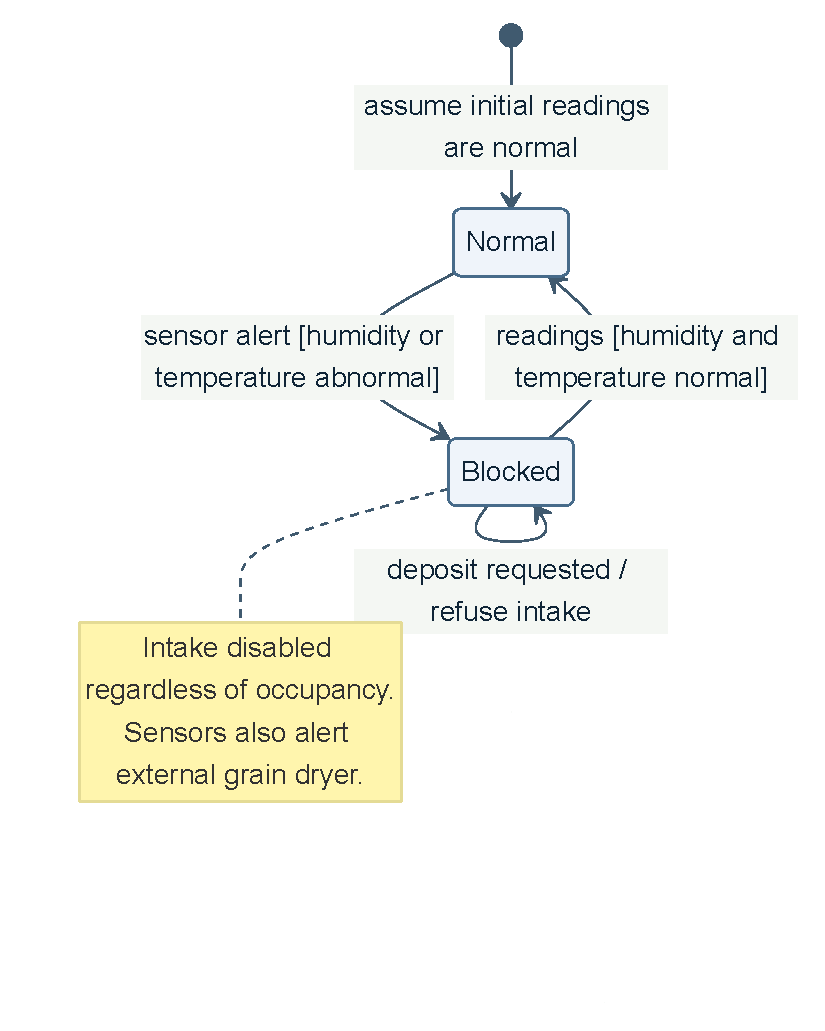
\includegraphics[width=239.91pt]{images/fig-041.pdf}
\captionof{figure}{14.5 Silo condition state machine (requirement E)}\end{minipage}\par\smallskip


The initial normal reading is a stated model assumption. Unknown initial readings and sensor-failure policy remain TBD. ``Intake disabled'' is a constraint; \code{refuse intake} is an event response, not a continuously running \code{do/\allowbreak{}} activity. Returning to Normal removes the sensor block; capacity and type/\allowbreak{}grade constraints still apply.


\subsection*{14.6 Hard arrival invariant}
\textbf{Plan, then record reality:} offer load; compute eligible silo proposal; accept/overrule; unload; report actual amounts and shipment details; update stock/log; acknowledge. Routine class/use-case/sequence drawings are omitted here; the invariants above are the part that cannot be copied blindly from a generic model.
\end{studycolumns}

\chapteropen{Chapter 15: Hard tutorial questions}{chapter-15}
\markboth{Ch. 15 | Hard tutorials}{}


\begin{studycolumns}
\vspace{0pt}
\begin{eli5box}The hard part is keeping two independent changes separate: which plants want an event, and how each plant receives it. A subscription list chooses who; a channel strategy chooses how.\end{eli5box}
\textbf{Other hard exercises, answered once:} Tutorial 8's normal/sensor-range ECs and ambiguous below-normal policy are in Section 13.9. Tutorial 9's compound conditions, feasible traces and two-test coverage suite are in Section 12.9. The routine projector and basic tutorial walkthroughs are omitted.
\end{studycolumns}
\Needspace{100pt}
\subsection*{Hard tutorial: selective Observer + channel Strategy}
\begin{studycolumns}
\sectionlabel{h-tutorial-7--observer--factory}
\textbf{Q1.} GES notifies processing plants on grain arrival/\allowbreak{}departure; plants register \textbf{interests in specific grain types}; notification via preferred channel \textbf{email, SMS, or both}; interests and channels \textbf{vary over time}; must be \textbf{easily extended} to new channels.

\begin{itemize}
\item \textbf{Design problem:} one-to-many notification with runtime-variable subscribers and \emph{two} varying dimensions (interest + channel).
\item \textbf{Patterns:} \textbf{Observer} (subscription + notification: \code{attach/\allowbreak{}detach/\allowbreak{}notify}, \code{update} with interests \ensuremath{\rightarrow} \textbf{selective notification}) \textbf{+ Strategy} for the communication means (\code{Email\allowbreak{}Notifier}, \code{SMSNotifier}, \code{Composite\allowbreak{}Notifier} for "both") \textbf{+ an optional Factory} to create the notifier for a plant's current preference.
\item \textbf{Trap:} "combination of these means" \ensuremath{\Rightarrow} the \textbf{Composite} pattern is also defensible for email+SMS; say so and justify.
\end{itemize}
\end{studycolumns}


\par\smallskip\noindent\begin{minipage}{\linewidth}\centering
\begin{minipage}[t]{0.488\linewidth}\centering\scriptsize\textbf{1}\par\smallskip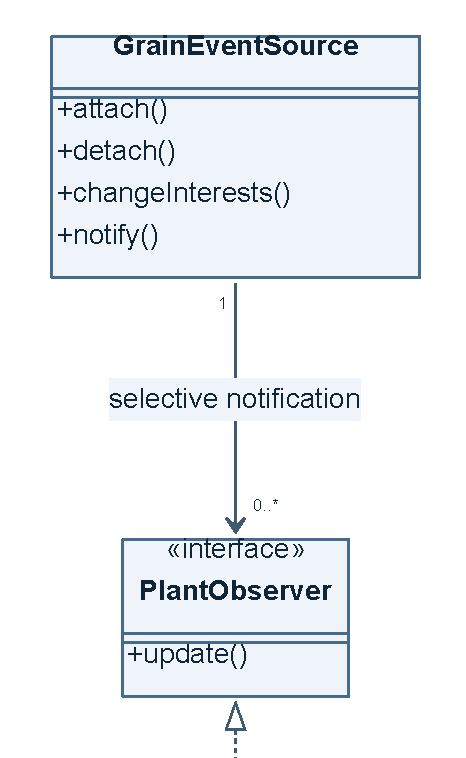
\includegraphics[width=137.08pt]{images/fig-046-compact-1.pdf}\end{minipage}\hfill
\begin{minipage}[t]{0.488\linewidth}\centering\scriptsize\textbf{2}\par\smallskip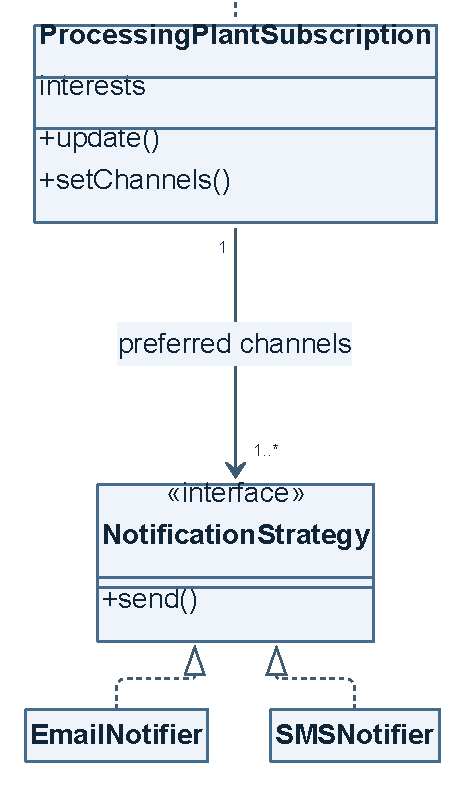
\includegraphics[width=137.08pt]{images/fig-046-compact-2.pdf}\end{minipage}
\captionof{figure}{Hard tutorial: selective Observer + channel Strategy --- follow numbered panels; crossing arrows continue.}\end{minipage}\par\smallskip



\textbf{Channel check:} interests and delivery channels change independently. Send through each selected channel so ``both'' is supported; channel creation may use an optional Factory.


\chapteropen{Chapter 16: AI engineering and agentic systems}{chapter-16}
\markboth{Ch. 16 | AI systems}{}


\begin{studycolumns}
\vspace{0pt}
\begin{eli5box}
Treat an LLM like a fluent assistant who can still misunderstand the task. It can suggest code, tests or tags, but another part of the system must check the result. Asking the assistant to promise 'I am correct' is not the same as measuring correctness.
\end{eli5box}
\textbf{Answer check:} Separate LLM proposals from deterministic validators, policy gates and execution. Valid JSON can still have a wrong shape, disallowed tags or too many tags. An LLM-selected role does not authenticate a user; agent agreement does not prove passing tests.
\end{studycolumns}


\par\smallskip\noindent\begin{minipage}{\linewidth}\centering
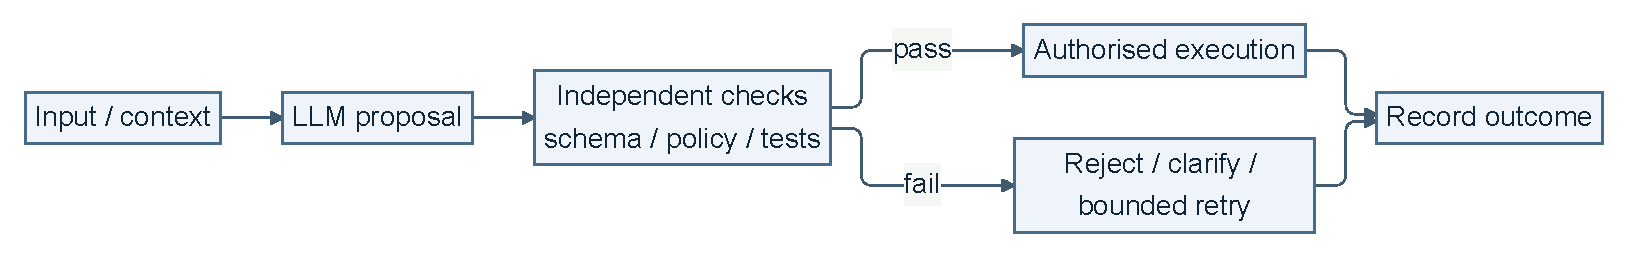
\includegraphics[width=479.32pt]{images/extra-trust.pdf}
\captionof{figure}{LLM outputs need independent checks; generation is not verification}\end{minipage}\par\smallskip

\begin{studycolumns}
\vspace{0pt}



\needspace{4\baselineskip}
\subsection*{16.1 AI engineering vocabulary}
\sectionlabel{h-161-ai-engineering-vocabulary}

\begin{referenceentries}
\textit{\textbf{Term} / \textbf{Definition}}\par\smallskip
\noindent \textbf{\textbf{AI engineering}}: The discipline of \textbf{building, deploying and maintaining AI-powered systems} in the real world; it fuses AI research (what is possible), software engineering (what works reliably) and domain expertise (what matters)\par
\noindent \textbf{\textbf{AI vs ML vs DL}}: AI = broad science of mimicking human abilities; ML = algorithms that improve through experience; DL = multi-layer neural networks for complex patterns\par
\noindent \textbf{\textbf{AI engineering vs ML engineering}}: The guest decks contrast traditional model development/\allowbreak{}training with applications built on foundation models; treat this as a focus distinction, not an exclusive definition\par
\noindent \textbf{\textbf{LLM pipeline}}: Tokenisation \ensuremath{\rightarrow} embeddings \ensuremath{\rightarrow} attention \ensuremath{\rightarrow} next-token prediction \ensuremath{\rightarrow} (training adjusted the weights)\par
\noindent \textbf{\textbf{RAG}}: Retrieval-augmented generation: fetch relevant documents, then generate grounded on them\par
\noindent \textbf{\textbf{Agent}}: Plans and executes a \textbf{sequence of actions} to achieve a goal --- plans across steps, keeps state/\allowbreak{}memory, uses tools, loops until done (vs a stateless, one-shot chatbot)\par
\noindent \textbf{\textbf{ReAct loop}}: THINK \ensuremath{\rightarrow} ACT \ensuremath{\rightarrow} OBSERVE \ensuremath{\rightarrow} THINK \ldots{} with tools, memory, and a \textbf{condition} for termination\par
\noindent \textbf{\textbf{MCP}}: Model Context Protocol --- standard way to expose tools/\allowbreak{}context to models\par
\noindent \textbf{\textbf{Agent risks}}: infinite loops \ensuremath{\cdot} \textbf{indirect prompt injection} \ensuremath{\cdot} \textbf{irreversible actions}\par
\end{referenceentries}
\needspace{4\baselineskip}
\subsection*{16.2 AI failure modes worth remembering}
\sectionlabel{h-162-ai-failure-modes-worth-remembering}

\begin{referenceentries}
\textit{\textbf{Failure} / \textbf{Description}}\par\smallskip
\noindent \textbf{\textbf{Hallucination}}: Confidently stating factually wrong things (e.g. non-existent case citations)\par
\noindent \textbf{\textbf{Bias}}: Amplifying historical discrimination (e.g. a hiring model downgrading r\'{e}sum\'{e}s)\par
\noindent \textbf{\textbf{Prompt injection}}: Malicious instructions hidden in content the model reads (direct vs \textbf{indirect})\par
\noindent \textbf{\textbf{Over-reliance}}: Automation bias --- humans stop checking the output\par
\end{referenceentries}
\textbf{Evaluation challenges:} natural complexity \ensuremath{\cdot} open-ended tasks with multiple valid answers \ensuremath{\cdot} black-box nature \ensuremath{\cdot} benchmark saturation \ensuremath{\cdot} emerging capabilities.

\needspace{4\baselineskip}
\subsection*{16.3 TDD vs BDD vs SDD (the one comparison worth knowing)}
\sectionlabel{h-163-tdd-vs-bdd-vs-sdd-the-one-comparison-worth-knowing}

\begin{referenceentries}
\textit{\textbf{Question it answers}}\par\smallskip
\noindent \textbf{\textbf{TDD} (test-driven development)}: \emph{How do you verify \textbf{one behaviour}?} Write a test first, then code to make it pass\par
\noindent \textbf{\textbf{BDD} (behaviour-driven development)}: \emph{How do \textbf{users/\allowbreak{}business} expect it to act?} Write scenarios in business language, implement against them\par
\noindent \textbf{\textbf{SDD} (spec-driven development)}: \emph{What should the \textbf{system} do?} Write the spec first, implement to match it\par
\end{referenceentries}
\textbf{The SDD loop:} \textbf{Discuss \ensuremath{\rightarrow} Specify \ensuremath{\rightarrow} Delegate \ensuremath{\rightarrow} Evaluate}, with a \textbf{human review checkpoint} for every submitted change. Anti-pattern: \emph{vibe coding} --- vague request \ensuremath{\rightarrow} plausible code \ensuremath{\rightarrow} hope ("fragile \& ungrounded").

\textbf{Mapping back onto SC2006 (the useful part):}


\begin{referenceentries}
\textit{\textbf{SDD phase} / \textbf{SC2006 equivalent}}\par\smallskip
\noindent \textbf{Discuss}: Requirements \textbf{elicitation} (interview/\allowbreak{}workshop, learn the problem domain, name what is out of scope)\par
\noindent \textbf{Specify}: \textbf{SRS} + use case descriptions + data dictionary (the "written spec that survives the session")\par
\noindent \textbf{Delegate}: Implementation (object design \ensuremath{\rightarrow} code)\par
\noindent \textbf{Evaluate}: \textbf{Validation \& verification}, acceptance testing, UAT\par
\end{referenceentries}


\par\smallskip{\color{line}\hrule}\smallskip
\needspace{4\baselineskip}
\subsection*{16.4 AI engineering practice: adapting, evaluating and operating systems}
\sectionlabel{h-164-ai-engineering-practice-adapting-evaluating-and-operating-systems}
The practice deck develops three layers: \textbf{application development} (interface, prompts, context, evaluation), \textbf{model development} (adaptation/\allowbreak{}training, datasets, inference optimisation, evaluation) and \textbf{infrastructure} (compute/\allowbreak{}data management, serving, monitoring).

\begin{itemize}
\item \textbf{Prompt engineering:} specify task, instructions, examples and context. Fast to change; it does not update the model's weights or make unsupported output automatically correct.
\item \textbf{RAG:} retrieve relevant external documents and supply them as generation context. Useful for private or changing knowledge; retrieval quality, latency and document maintenance still matter.
\item \textbf{Fine-tuning:} adapt model weights using suitable labelled examples for a narrow task or desired behaviour. It needs data and training effort; distinguish it from adding context at inference time.
\item \textbf{Evaluation:} use representative tests and quantitative/\allowbreak{}qualitative review throughout development, including component tests and end-to-end behaviour. The Understanding deck also covers fairness, privacy, hallucination, prompt injection and monitoring after deployment.
\item \textbf{Operations:} the practice deck includes REST APIs, containerised dependencies, Kubernetes for orchestration, and CI/\allowbreak{}CD/\allowbreak{}continuous training. Architecture combines the application, model, retrieval/\allowbreak{}data and serving layers; no single tool guarantees quality.
\end{itemize}
The agentic-development deck adds \textbf{automated}, \textbf{observed} and \textbf{human} evaluation evidence: unit/\allowbreak{}integration tests, type checks/\allowbreak{}lint/\allowbreak{}builds; runtime/\allowbreak{}UI behaviour and logs; requirements traceability, diff review, security/\allowbreak{}privacy/\allowbreak{}maintainability. It advocates short feedback loops, enforced checks and searchable structured logs. Passing those checks establishes only what the checks cover, not absence of bugs.

\needspace{4\baselineskip}
\subsection*{16.5 Architecture extension in the Thursday system-design deck}
\sectionlabel{h-165-architecture-extension-in-the-thursday-system-design-deck}
\code{Lecture\_\allowbreak{}12\_\allowbreak{}System\_\allowbreak{}Design\_\allowbreak{}2026\_\allowbreak{}Thursday.\allowbreak{}pdf}, pp. 8--14, discusses intelligence, a three-level capability system (\textbf{foundational, integrative, applied}), LLM agent architecture and brain-inspired agent architecture. These are exploratory architecture examples, not new GES requirements or additional GoF patterns. Their assessment status is not stated in the files.
\end{studycolumns}

\chapteropen{Chapter 17: Examination answer checklist}{chapter-17}
\markboth{Ch. 17 | Exam playbook}{}


\begin{studycolumns}
\vspace{0pt}
\begin{eli5box}
An open-book reference is a labelled toolbox, not a substitute for knowing which tool a question needs. Read the command word, find the right template, then fill it using this case's facts. Every answer should make the examiner's checking job easy.
\end{eli5box}

\subsection*{Final answer checks}
\begin{enumerate}
\item Use this paper's names, units, role permissions and constraints consistently across all four questions.
\item Diagram: external actors; goal names; correct arrows; multiplicities at both association ends; guarded decisions; bars for concurrency.
\item Design: justify each component/pattern against a case requirement; include a trade-off, not only a name.
\item Tests: valid baseline, exactly one invalid field per defensive row, exact boundary equality and an independently justified expected result.
\end{enumerate}
\textbf{Pattern answer template:} Problem [what must vary]; pattern [name and mechanism]; roles [case classes]; consequence [benefit and cost].
\needspace{4\baselineskip}
\subsection*{Command-word decoder for exam prompts}
\sectionlabel{h-1712-common-word-decoder-for-exam-prompts}

\begin{referenceentries}
\textit{\textbf{Prompt says} / \textbf{They want}}\par\smallskip
\noindent \textbf{"Atomise"}: Numbered, single-assertion, verifiable statements\par
\noindent \textbf{"Identify the design problem"}: The \emph{smell} + the \emph{force}, before any pattern name\par
\noindent \textbf{"Apply the appropriate pattern"}: Name + class diagram + role table\par
\noindent \textbf{"Systematically design test cases"}: A \textbf{table} with one row per test case and an oracle column\par
\noindent \textbf{"Discuss"}: Two sides + a verdict + a trade-off\par
\noindent \textbf{"With justification"}: One sentence of \emph{why} per decision\par
\noindent \textbf{"Draw"}: Correct \textbf{notation}, not prose\par
\end{referenceentries}

\par\smallskip{\color{line}\hrule}\smallskip
\end{studycolumns}

\phantomsection\addcontentsline{toc}{section}{Source index}\section*{Source index}\label{source-notes}

\begin{studycolumns}
\vspace{0pt}
Lecture citations (L1--L18), tutorial numbers and section references throughout identify the evidence. All source PDFs are in the adjacent \code{lectures/}, \code{tutorial/} and \code{pyps/} folders. The editable study guide is \code{../SC2006\_Study\_Guide.md}.
\begin{itemize}
\item \textbf{Chapters 1--6:} Introduction; Requirements Elicitation 1--3; Conceptual Models; Dynamic Models; Writing SRS; UMLSpecNotes.
\item \textbf{Chapters 7--8:} Software Processes -- Basics; Agile Software Development -- Basics, including its image slides.
\item \textbf{Chapters 9--11:} System Design (both decks), Object Design (both decks), Design Patterns, MVC (both versions). The file named \code{Lecture\_13\_System\_Design\_2026.pdf} opens as Object Design.
\item \textbf{Chapters 12--13:} Test Fundamentals/Testing Introduction; Equivalence Class Testing; Boundary Value Testing (2026 and other supplied versions).
\item \textbf{Chapters 14--15:} Tutorial Questions and the scanned GES supplement. Tutorial-only examples remain in Chapter 15; shared answers appear once in their topic chapter.
\item \textbf{Chapter 16:} Understanding AI Engineering; AI Engineering as a practice -- NTU; Agentic Software Engineering; Thursday System Design extension. These guest topics have no separately confirmed assessment status in the supplied files.
\end{itemize}
\textbf{Source conflicts:} use hollow-triangle UML generalization; keep the course's historical Scrum wording distinct from current-standard claims; distinguish graph bases from feasible traces; use the problem's stated mortgage upper limit (8000 versus 80000); \code{800001} in the separate summary is a typo for \code{80001}. Full BV triplets and reduced course selections are labelled separately. Local GES and paper-specific assumptions remain beside the relevant answer.
\end{studycolumns}

\section*{Past-year papers and worked answers}\label{papers-start}
\fontsize{9}{10.5}\selectfont

\textbf{Paper format observed:} two hours, four compulsory 25-mark questions. Budget about 30 minutes per question, including reading/checking. The linked originals supply exact wording and Appendix A; prompts here are summaries. Worked designs are examples, not unique solutions.

{\fontsize{8.5}{9.8}\selectfont
\begin{longtable}{L{\dimexpr 0.37840\linewidth-9.08pt\relax}L{\dimexpr 0.20818\linewidth-5.00pt\relax}L{\dimexpr 0.41343\linewidth-9.92pt\relax}}
\toprule
\rowcolor{ice}\textbf{Paper} & \textbf{Scenario} & \textbf{Main modelling variation} \\
\midrule\endfirsthead
\toprule\rowcolor{ice}\textbf{Paper} & \textbf{Scenario} & \textbf{Main modelling variation} \\
\midrule\endhead
\multicolumn{3}{r}{\scriptsize Continued on next page}\\\endfoot
\bottomrule\endlastfoot
\href{run:/Users/bryangoh/Work/ntu-cs/sc2006/pyps/SC2006\_AY2223\_S1\_Questions.pdf}{AY2022/\allowbreak{}23 S1} & Car sales & Hold-car use case, conceptual classes, dialog map \\
\href{run:/Users/bryangoh/Work/ntu-cs/sc2006/pyps/SC2006\_AY2223\_S2\_Questions.pdf}{AY2022/\allowbreak{}23 S2} & Shopping chatbot & Replacement use case, conceptual classes, activity diagram \\
\href{run:/Users/bryangoh/Work/ntu-cs/sc2006/pyps/SC2006\_AY2324\_S1\_Questions.pdf}{AY2023/\allowbreak{}24 S1} & DevSecOps & Security-check use case, classes, activity diagram \\
\href{run:/Users/bryangoh/Work/ntu-cs/sc2006/pyps/SC2006\_AY2324\_S2\_Questions.pdf}{AY2023/\allowbreak{}24 S2} & CodeAgent & Reviewer use case, classes, QA-Checker state machine \\
\href{run:/Users/bryangoh/Work/ntu-cs/sc2006/pyps/SC2006\_AY2425\_S1\_Questions.pdf}{AY2024/\allowbreak{}25 S1} & Task management & Assignment use case, classes, task lifecycle activity diagram \\
\href{run:/Users/bryangoh/Work/ntu-cs/sc2006/pyps/SC2006\_AY2425\_S2\_Questions.pdf}{AY2024/\allowbreak{}25 S2} & Disaster Warning System & Stakeholders/\allowbreak{}requirements, sensor state machine, linking activity \\
\href{run:/Users/bryangoh/Work/ntu-cs/sc2006/pyps/SC2006\_AY2526\_S1\_Questions.pdf}{AY2025/\allowbreak{}26 S1} & Smart home & Guest access use case, controller state machine, voice activity \\
\href{run:/Users/bryangoh/Work/ntu-cs/sc2006/pyps/SC2006\_AY2526\_S2\_Questions.pdf}{AY2025/\allowbreak{}26 S2} & Restaurant recommendations & JSON-check activity, recommendation classes, conversation state machine \\
\end{longtable}
}
\textbf{Common testing conventions:} reset/isolate rows; keep fixtures and other inputs valid; combine valid coverage but use exactly one invalid field per defensive row. Accept means input validation passes, not that later external operations succeed. Reject means controlled failure without data mutation/crash. Oracles come from requirements; unclear behaviour is labelled TBD. Full triplets are retained; categorical membership has no numeric boundary.

\textbf{Answer map:} Q1 uses Chapters 2--3; modelling uses 4--5; process/Scrum uses 7--8; architecture/patterns uses 9--11; testing uses 12--13; AI checks use 16. Apply the method to the case rather than copying an earlier case's classes or limits.

\textbf{Drawing convention:} Mermaid approximates UML use-case/activity notation. In an examination, use UML actors, boundaries, ellipses, arrowheads, initial/final nodes, bars and guarded diamonds as explained in Chapters 3--5.


\section*{Older papers: grouped question bank}\label{older-bank}
\phantomsection\addcontentsline{toc}{section}{Older papers: cases and question map}
\markboth{Older papers | Case map}{}
The four older papers (AY2022/23 and AY2023/24) are grouped by question type. Each case retains its own prompt, diagrams, constraints and testing rows. The four newer papers follow in chronological order.

\begin{longtable}{L{.28\linewidth}L{.14\linewidth}L{.14\linewidth}L{.14\linewidth}L{.14\linewidth}}
\toprule\rowcolor{ice}\textbf{Older case} & \textbf{Q1} & \textbf{Q2} & \textbf{Q3} & \textbf{Q4}\\\midrule\endhead
Car sales & p.\ \pageref{old-2223-s1-q1} & p.\ \pageref{old-2223-s1-q2} & p.\ \pageref{old-2223-s1-q3} & p.\ \pageref{old-2223-s1-q4}\\
Shopping chatbot & p.\ \pageref{old-2223-s2-q1} & p.\ \pageref{old-2223-s2-q2} & p.\ \pageref{old-2223-s2-q3} & p.\ \pageref{old-2223-s2-q4}\\
DevSecOps & p.\ \pageref{old-2324-s1-q1} & p.\ \pageref{old-2324-s1-q2} & p.\ \pageref{old-2324-s1-q3} & p.\ \pageref{old-2324-s1-q4}\\
CodeAgent & p.\ \pageref{old-2324-s2-q1} & p.\ \pageref{old-2324-s2-q2} & p.\ \pageref{old-2324-s2-q3} & p.\ \pageref{old-2324-s2-q4}\\
\bottomrule
\end{longtable}
\begin{studycolumns}
\subsection*{AY2022/23 S1: Car sales}\label{paper-2223-s1}
\sectionlabel{h-161-ay202223-semester-1--car-selling-system-x}
\textbf{Source:} \href{run:/Users/bryangoh/Work/ntu-cs/sc2006/pyps/SC2006\_AY2223\_S1\_Questions.pdf}{Question paper}, Q1--Q4 on PDF pp. 1--3; Appendix A on p. 4.

\textbf{Case facts.} Visitors browse/\allowbreak{}search new and used cars. A registered, logged-in user can hold one car by paying a deposit through the dealer's payment system. A car has only one holder at a time; another user cannot hold or buy it. Cancellation/\allowbreak{}expiry causes a refund. A buyer completes purchase with dealer staff. Staff log in, view car information, manage orders and complete delivery only after full-payment confirmation. A sales manager additionally manages car listings and generates sales reports.
\subsection*{AY2022/23 S2: Shopping chatbot}\label{paper-2223-s2}
\sectionlabel{h-162-ay202223-semester-2--customer-service-chatbot}
\textbf{Source:} \href{run:/Users/bryangoh/Work/ntu-cs/sc2006/pyps/SC2006\_AY2223\_S2\_Questions.pdf}{Question paper}, Q1--Q4 on PDF pp. 1--4; Appendix A on p. 5.

\textbf{Case facts.} The chatbot answers product/\allowbreak{}pricing/\allowbreak{}availability queries and helps logged-in customers manage carts, orders, payment/\allowbreak{}delivery details, status, replacements and refunds. Free replacement/\allowbreak{}refund is available within seven days of delivery, with item photos, purchase receipt and reasons. The company confirms or rejects the request; the chatbot communicates instructions or rejection.
\subsection*{AY2023/24 S1: DevSecOps}\label{paper-2324-s1}
\sectionlabel{h-171-ay202324-semester-1--devsecops-platform}
\textbf{Source:} \href{run:/Users/bryangoh/Work/ntu-cs/sc2006/pyps/SC2006\_AY2324\_S1\_Questions.pdf}{Question paper}, Q1--Q4 on PDF pp. 1--3; Appendix A on p. 4.

\textbf{Case facts.} A developer supplies a local project or GitHub link. The platform analyses security and quality using four external toolsets: SCA, SAST, DAST and IAST. It generates a report and offers mitigation recommendations. Project-selection help is optional. Developers may rerun selected toolsets to verify fixes and generate reports on request.
\subsection*{AY2023/24 S2: CodeAgent}\label{paper-2324-s2}
\sectionlabel{h-172-ay202324-semester-2--codeagent}
\textbf{Source:} \href{run:/Users/bryangoh/Work/ntu-cs/sc2006/pyps/SC2006\_AY2324\_S2\_Questions.pdf}{Question paper}, Q1--Q4 on PDF pp. 1--4; Appendix A on p. 5.

\textbf{Case facts.} Seven internal agents are User, CEO, CPO, CTO, Reviewer, Coder and QA-Checker. The first six correspond to user roles; users log in to interact with the corresponding agents. Code review recognises input modality/\allowbreak{}language; Reviewer checks commit-message consistency, vulnerability injection and formatting; Coder revises code; Coder/\allowbreak{}CTO/\allowbreak{}CEO summarise the work. Paired agents converse under QA-Checker supervision until the answer is appropriate or a dialogue limit is reached. Logs/\allowbreak{}reports are generated on request.
\end{studycolumns}

\fontsize{9}{10.5}\selectfont
\par\Needspace{100pt}\section*{Older Q1: Use-case models and descriptions}\label{older-q1}
\phantomsection\addcontentsline{toc}{section}{Older Q1: Use-case models and descriptions}
\markboth{Older papers | Q1}{}
\textbf{Shared method:} use the boundary/relationship and description checks in Chapter 3, p.\ \pageref{chapter-3}. Each case retains its own actors, flow and failure rules.
\par\Needspace{85pt}\subsection*{AY2022/23 S1: Car sales --- Q1 (25 marks)}\label{old-2223-s1-q1}

\sectionlabel{h-q1--use-cases-25-marks}
\textbf{(a) Identify actors/\allowbreak{}use cases and draw their relationships (17). (b) Describe holding a car: actors, preconditions, flow and alternatives (8).}


\textbf{(a)} Actors: Visitor, Registered Customer, Dealer Staff, Sales Manager and external Dealer Payment System. Registered Customer can do the visitor's browsing; Sales Manager inherits staff capabilities. The system itself, its database and a car are not actors.





\par\smallskip\noindent\begin{minipage}{\linewidth}\centering
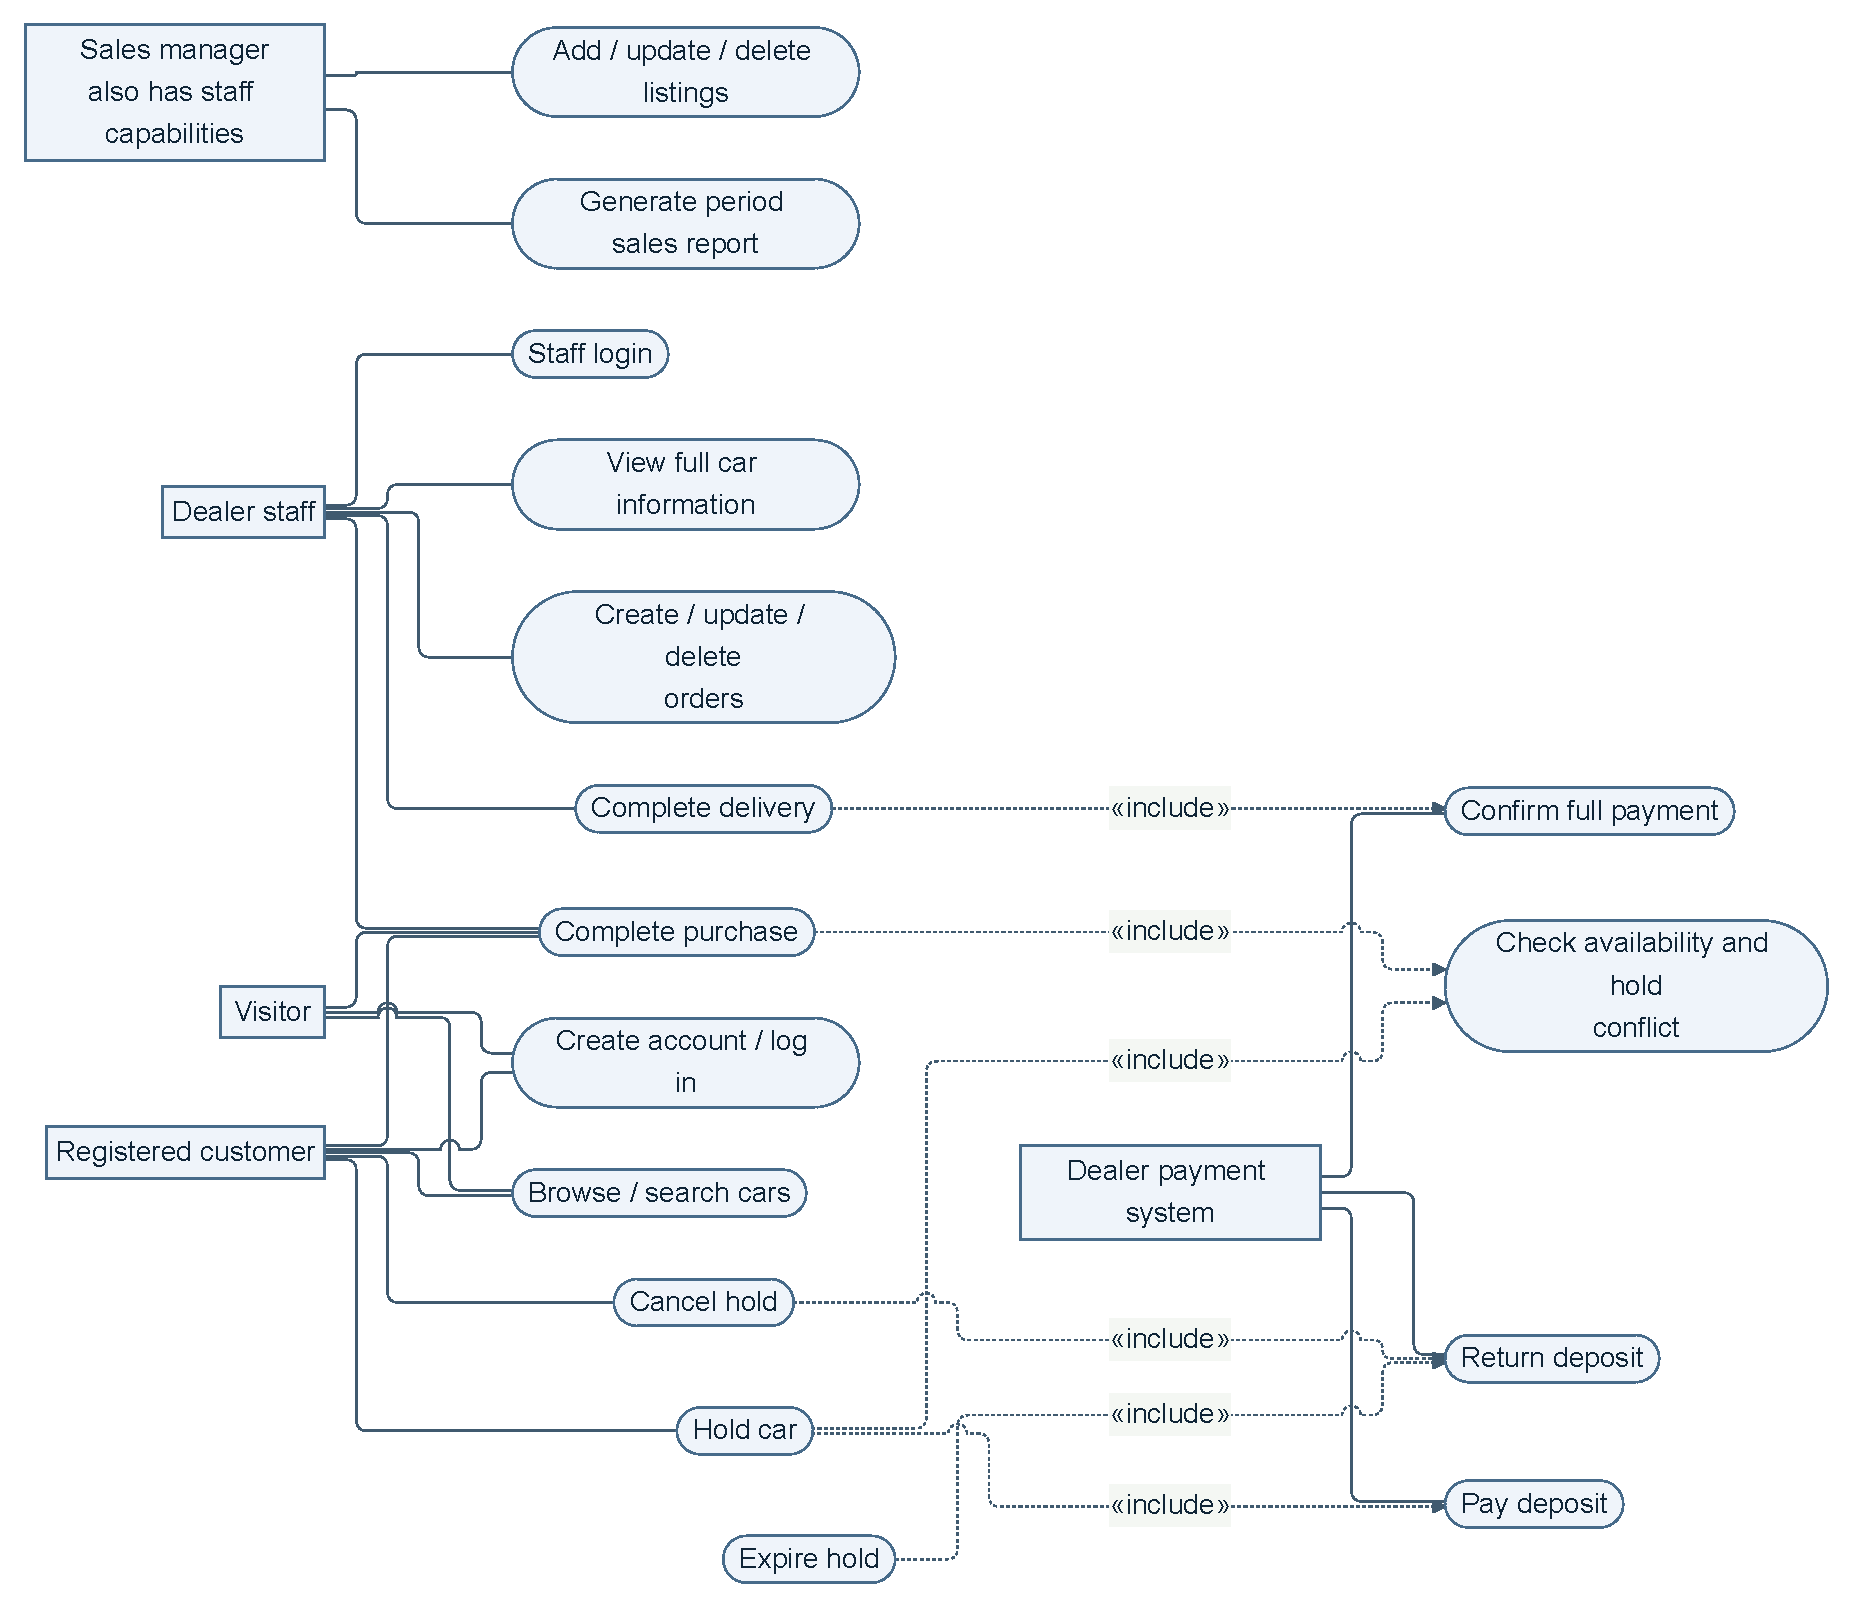
\includegraphics[width=506.64pt]{images/fig-048.pdf}
\captionof{figure}{Car sales: Q1 --- Use cases (25 marks)}\end{minipage}\par\smallskip

\begin{studycolumns}
\vspace{0pt}




Generalization: Customer to Visitor; Sales Manager to Staff. Expiry is an internally scheduled system action; a timer need not be invented as an external actor. The appendix does not explicitly require an account/\allowbreak{}deposit for a direct purchase with staff; those requirements apply to holding a car. A failed deposit is an alternative flow. The question says use relationships \textbf{where appropriate}, so an artificial extension is unnecessary.

\textbf{(b) Use case: Hold Car.} Primary actor: Registered Customer. Supporting actor: Dealer Payment System. Preconditions: customer is authenticated; selected car exists, is unsold and is not already under an active hold. Normal flow:

\begin{enumerate}
\item Customer selects a car and requests a hold.
\item System checks current availability and displays deposit/\allowbreak{}hold terms. The duration and deposit amount come from dealer policy; the paper gives no numbers.
\item Customer confirms and authorises the deposit through the payment system.
\item Payment system confirms success. System creates the hold for that customer and marks the car unavailable to other customers until expiry.
\item System displays the hold reference and expiry time.
\end{enumerate}
Alternatives: failed/\allowbreak{}cancelled payment creates no active hold; a concurrent hold/\allowbreak{}purchase causes rejection rather than double allocation; expiry or user cancellation ends the hold and requests a refund. A payment confirmed after an allocation conflict must be compensated/\allowbreak{}refunded. \textbf{Design assumption:} availability checks and allocation are made atomic, with a pending reservation/\allowbreak{}payment reconciliation mechanism. Do not imply that an initial availability check alone prevents races.
\end{studycolumns}

\par\Needspace{85pt}\subsection*{AY2022/23 S2: Shopping chatbot --- Q1 (25 marks)}\label{old-2223-s2-q1}


\begin{studycolumns}
\vspace{0pt}
\sectionlabel{h-q1--use-cases-25-marks-1}
\textbf{(a) Actors/\allowbreak{}use cases and relationships (17). (b) Item-replacement description with actors, preconditions, normal/\allowbreak{}alternative flows (8).}


\textbf{(a)} The chatbot is the system being modelled, not an external actor. Customer is the primary actor. Existing Web-Based Shopping System is a supporting actor outside the chatbot boundary; company approval is supplied through that system. If company staff directly operate a chatbot approval interface, they become another actor, but that interface is not specified.
\end{studycolumns}


\par\smallskip\noindent\begin{minipage}{\linewidth}\centering
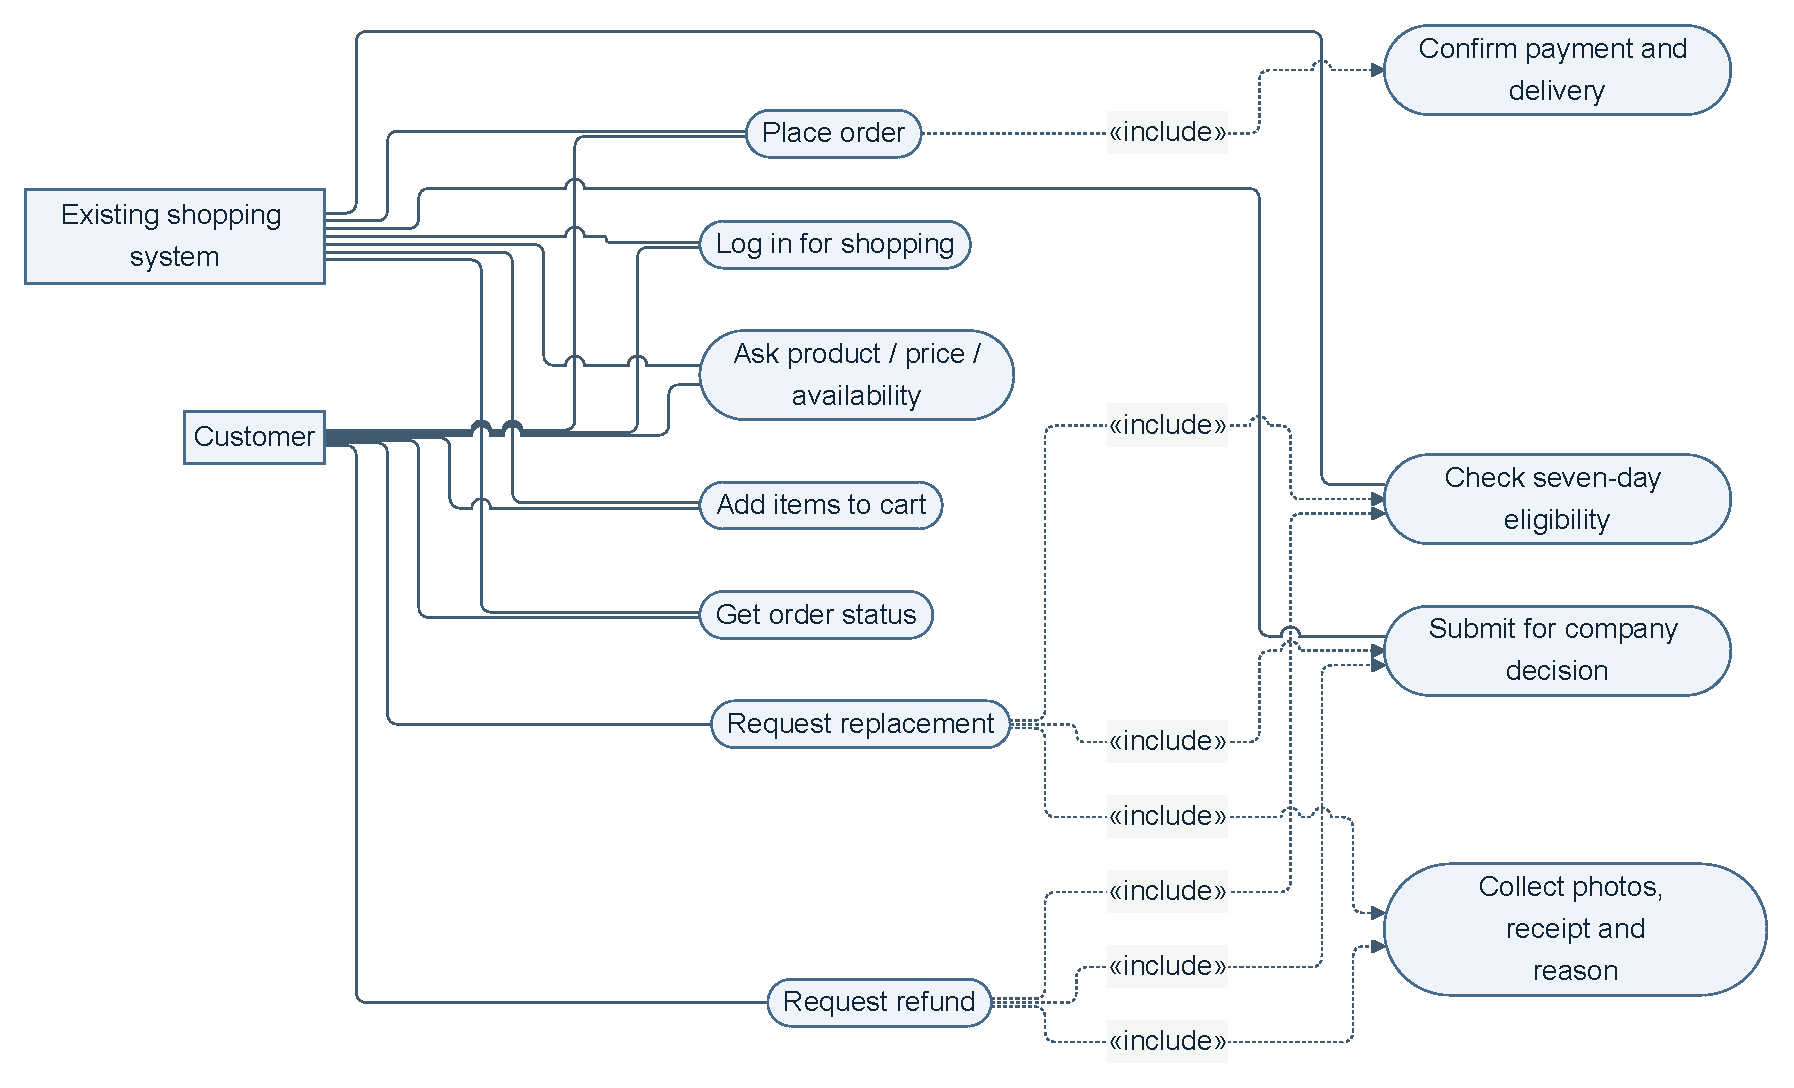
\includegraphics[width=461.44pt]{images/fig-053.pdf}
\captionof{figure}{Shopping chatbot: Q1 --- Use cases (25 marks)}\end{minipage}\par\smallskip

\begin{studycolumns}
\vspace{0pt}



Approval leads to replacement/refund instructions; rejection is an alternative flow. Shopping actions require a valid authenticated session, while product enquiries can precede login.

\textbf{(b) Use case: Request Item Replacement.} Actors: Customer, Existing Shopping System (including company decision service). Preconditions: customer is logged in; the delivered purchase can be identified. Normal flow:

\begin{enumerate}
\item Customer asks for replacement and selects the purchased item/\allowbreak{}order.
\item Chatbot retrieves purchase/\allowbreak{}delivery details and checks the seven-day rule.
\item Chatbot asks for item photos, receipt and replacement reason; customer supplies them.
\item Chatbot validates completeness and submits the request to the existing system for company confirmation.
\item On approval, chatbot sends the company-provided replacement procedure and request reference.
\end{enumerate}
Alternatives: outside the eligibility period, reject the free replacement; missing evidence, request correction; company rejects, communicate rejection; integration failure, report pending/\allowbreak{}failure without falsely confirming approval. \textbf{Assumption:} ``within seven days'' includes the seventh day; the exact timestamp/\allowbreak{}timezone policy needs agreement. Company review may be asynchronous, so ``submitted/\allowbreak{}pending'' is distinct from ``approved''.
\end{studycolumns}

\par\Needspace{85pt}\subsection*{AY2023/24 S1: DevSecOps --- Q1 (25 marks)}\label{old-2324-s1-q1}

\sectionlabel{h-q1--use-cases-25-marks-2}
\textbf{(a) Actors, use cases and relationships (17). (b) Describe the security-check functionality (8).}


\textbf{(a)} Primary actor: Developer. Supporting actors: external SCA/\allowbreak{}SAST/\allowbreak{}DAST/\allowbreak{}IAST services and GitHub for remote project retrieval. The platform's own scanner coordinator and report store are internal components, not actors.




\par\smallskip\noindent\begin{minipage}{\linewidth}\centering
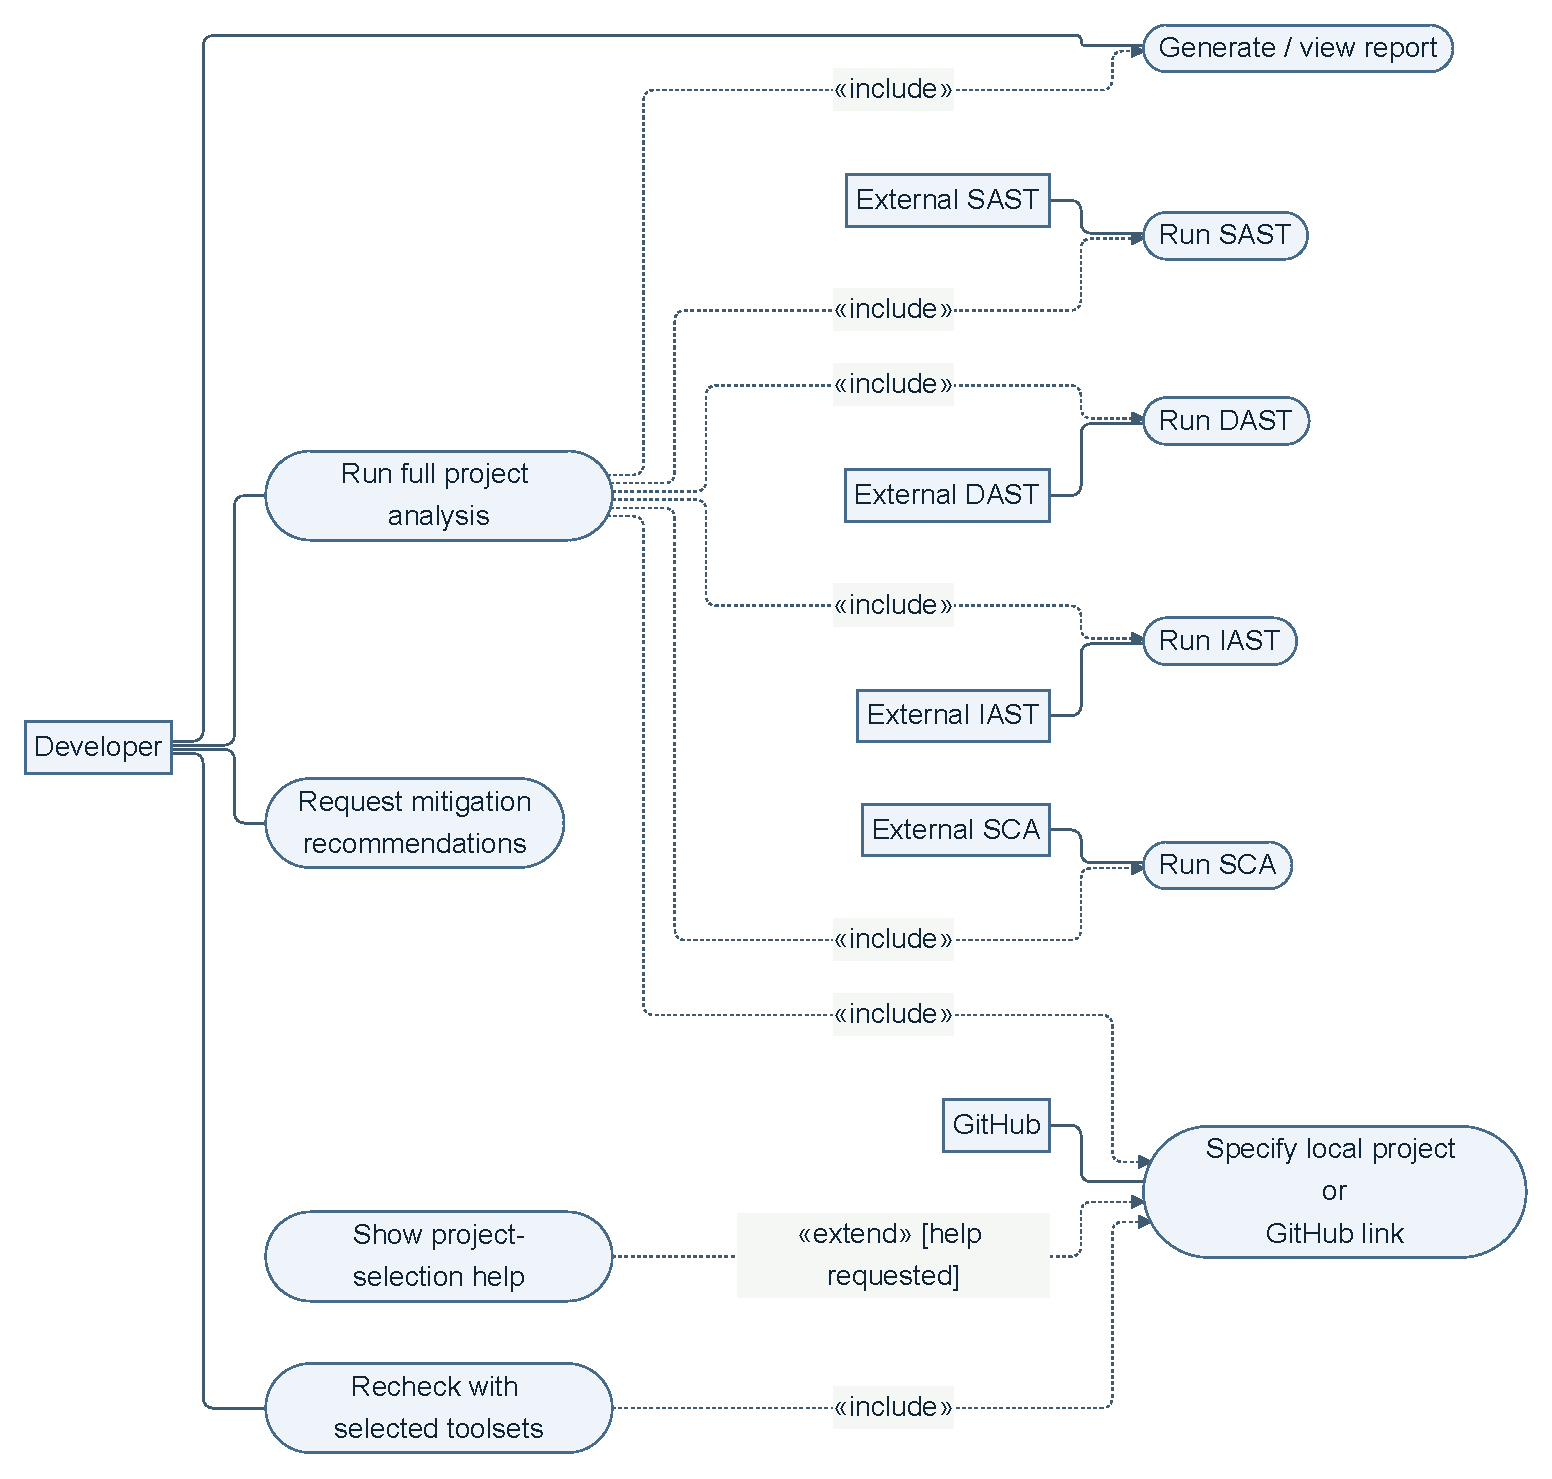
\includegraphics[width=436.92pt]{images/fig-058.pdf}
\captionof{figure}{DevSecOps: Q1 --- Use cases (25 marks)}\end{minipage}\par\smallskip

\begin{studycolumns}
\vspace{0pt}



Selected reruns invoke only chosen engines; the diagram's four mandatory includes apply to the \textbf{full-analysis} use case. GitHub participates only in the remote-source alternative. Mitigation is available after a report; it need not be automatically included in every scan. Selection help is a genuine optional extension.

\textbf{(b) Use case: Check Project Security.} Actors: Developer; selected external analysis toolsets; GitHub when applicable. Preconditions: project is accessible; required engines are available/\allowbreak{}configured. Normal flow:

\begin{enumerate}
\item Developer specifies local source or a GitHub link; platform obtains the project.
\item Platform runs all four toolsets for an initial full analysis, or the developer selects toolsets for a verification rerun.
\item Each selected toolset returns its findings; platform associates results with the project/\allowbreak{}version and combines them.
\item Platform generates and displays a security/\allowbreak{}quality report.
\item On request, platform supplies mitigation recommendations.
\end{enumerate}
Alternatives: developer requests selection help; inaccessible source produces a corrective message; unsupported/\allowbreak{}failed/\allowbreak{}timed-out engine is reported with explicit incomplete status, not a clean result; developer fixes issues and reruns selected checks. Version tagging and incomplete-result status are proposed design details needed for trustworthy results. The paper does not specify a login requirement, so do not invent one as a case fact.
\end{studycolumns}

\par\Needspace{85pt}\subsection*{AY2023/24 S2: CodeAgent --- Q1 (25 marks)}\label{old-2324-s2-q1}

\sectionlabel{h-q1--use-cases-25-marks-3}
\textbf{(a) Actors/\allowbreak{}use cases/\allowbreak{}relationships (19). (b) Reviewer-agent use case description (6).}


\textbf{(a)} With the \textbf{whole CodeAgent platform} as the system boundary, agents are internal software, not external human actors. Model the six corresponding external user roles and their authenticated interactions. Appendix wording is unusual; this boundary/\allowbreak{}role interpretation is explicit rather than silently treating every program as an actor.







\par\smallskip\noindent\begin{minipage}{\linewidth}\centering
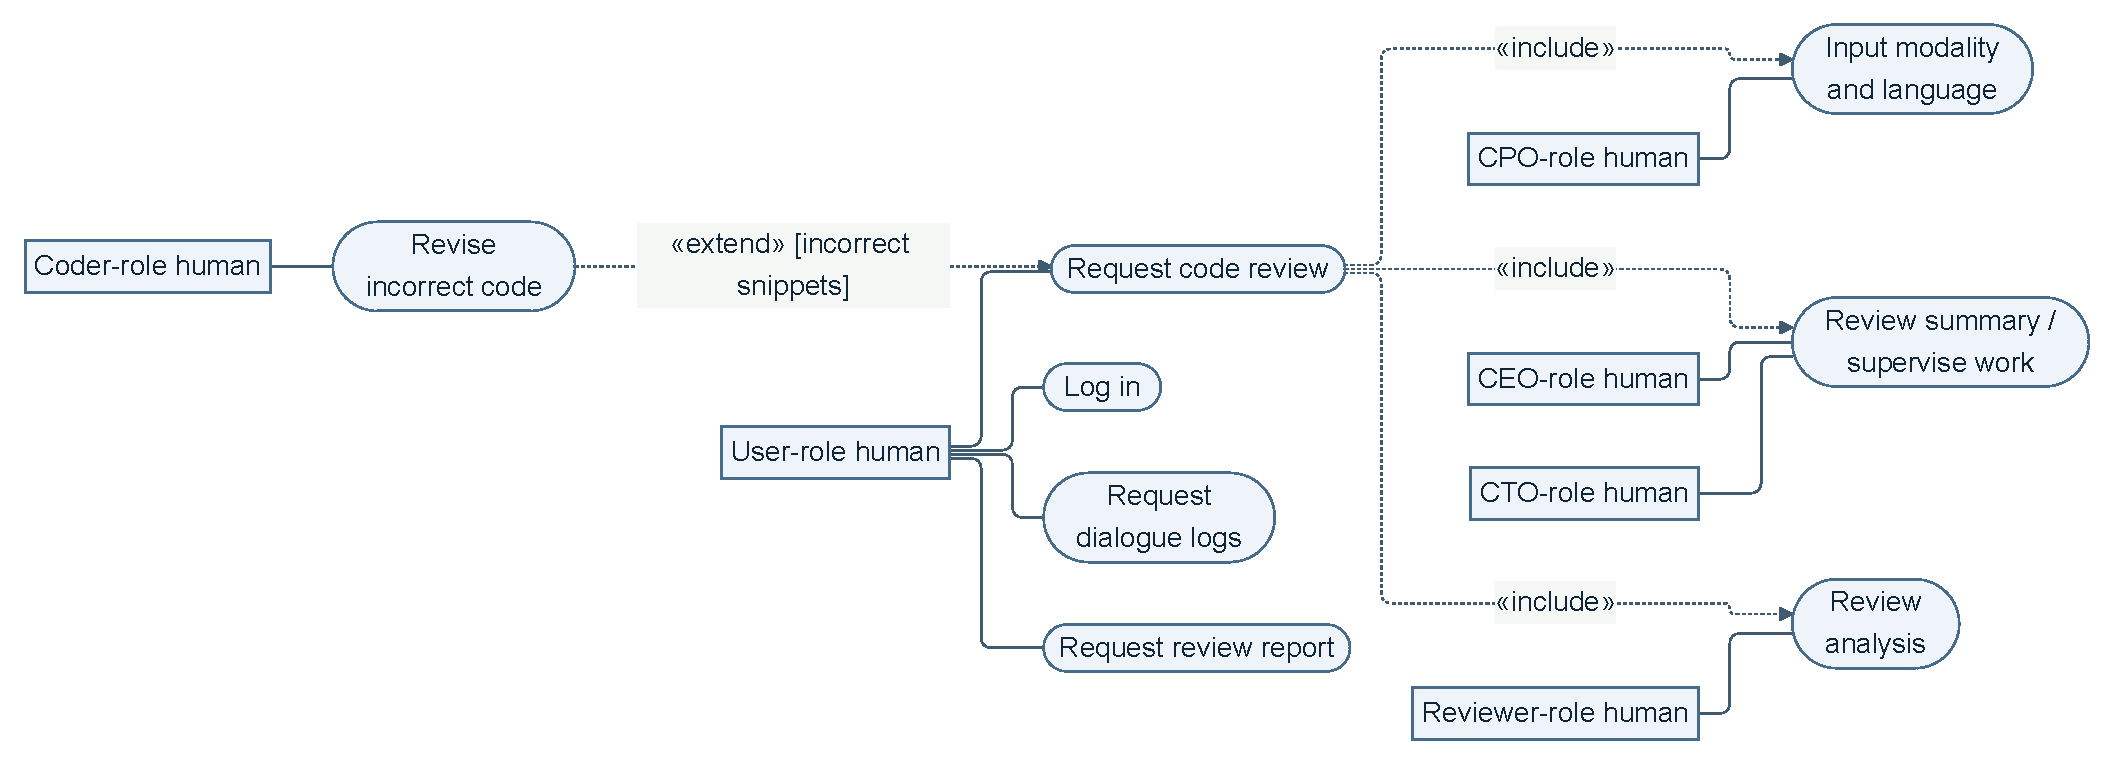
\includegraphics[width=514.00pt]{images/fig-063.pdf}
\captionof{figure}{CodeAgent: Q1 --- Use cases (25 marks)}\end{minipage}\par\smallskip





Detail view of the same \textbf{Perform review analysis} use case:




\par\smallskip\noindent\begin{minipage}{\linewidth}\centering
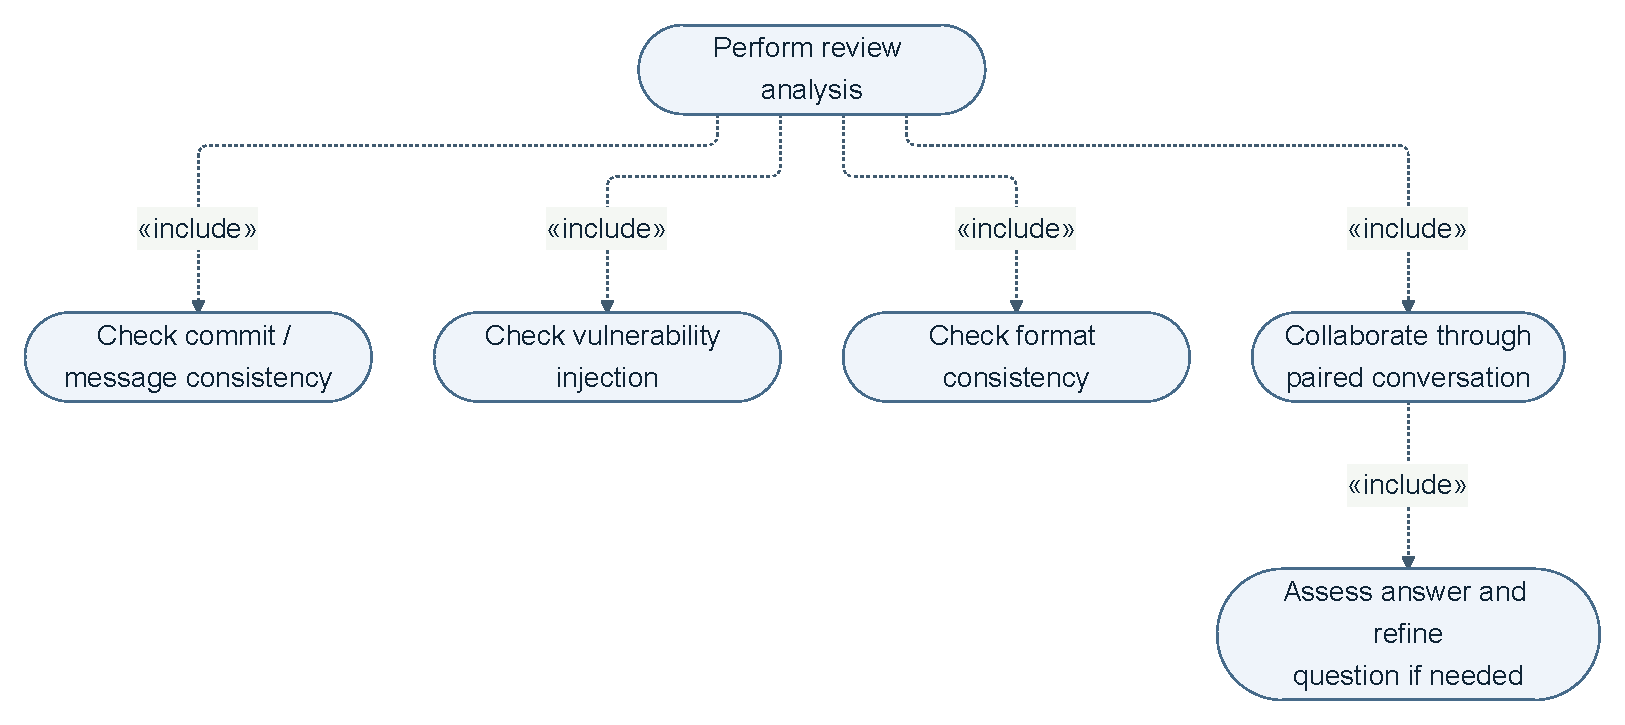
\includegraphics[width=457.60pt]{images/fig-064.pdf}
\captionof{figure}{CodeAgent: Q1 --- Use cases (25 marks)}\end{minipage}\par\smallskip

\begin{studycolumns}
\vspace{0pt}



All six role users can log in, interact with their corresponding agents, and request permitted outputs; show generalization to a common Authenticated User actor in exact UML rather than implying that only User-role humans log in. Internal CEO/\allowbreak{}CPO/\allowbreak{}Coder collaboration and Coder/\allowbreak{}CTO/\allowbreak{}CEO summarisation occur through agent orchestration; external users need not manually perform every subtask. QA-Checker needs no extra human actor.

\textbf{(b) Use case: Review Submitted Code.} Primary actor: authenticated requesting user/\allowbreak{}Reviewer-role user, according to the interface boundary chosen above. Preconditions: commit, commit message and original files are available; prior input recognition identifies modality/\allowbreak{}language. Flow: submit review request; Reviewer obtains code/\allowbreak{}context with Coder's help; analyse commit-message consistency, introduced vulnerabilities and formatting; conduct supervised conversations where needed; create an analysis report with observations and suggested revisions; provide it to Coder/\allowbreak{}user. Alternatives: missing/\allowbreak{}unreadable inputs, ask for correction; inappropriate answers, QA-Checker appends instructions and retries within the limit; limit exhausted, report unresolved/\allowbreak{}incomplete analysis rather than claiming success. Coder's subsequent revision is conditional on finding incorrect snippets.
\end{studycolumns}


\fontsize{9}{10.5}\selectfont
\par\Needspace{100pt}\section*{Older Q2: Conceptual models, behaviour and process}\label{older-q2}
\phantomsection\addcontentsline{toc}{section}{Older Q2: Conceptual models, behaviour and process}
\markboth{Older papers | Q2}{}
\textbf{Shared method:} apply Chapters 4--5 to the named object/workflow; use \hyperref[answer-waterfall]{W, p.\ \pageref{answer-waterfall}} and \hyperref[answer-scrum]{S, p.\ \pageref{answer-scrum}} for process questions.
\par\Needspace{85pt}\subsection*{AY2022/23 S1: Car sales --- Q2 (25 marks)}\label{old-2223-s1-q2}

\sectionlabel{h-q2--analysis-and-process-25-marks}
\textbf{(a) Hold-car conceptual classes with boundary/\allowbreak{}control/\allowbreak{}entity stereotypes (8). (b) Dialog map for holding a car (8). (c) Can customer involvement fix Waterfall's response to changing requirements? (4). (d) Estimate Scrum progress and timely completion (5).}


\textbf{(a)} The external payment system is represented by a payment boundary, not an entity.




\par\smallskip\noindent\begin{minipage}{\linewidth}\centering
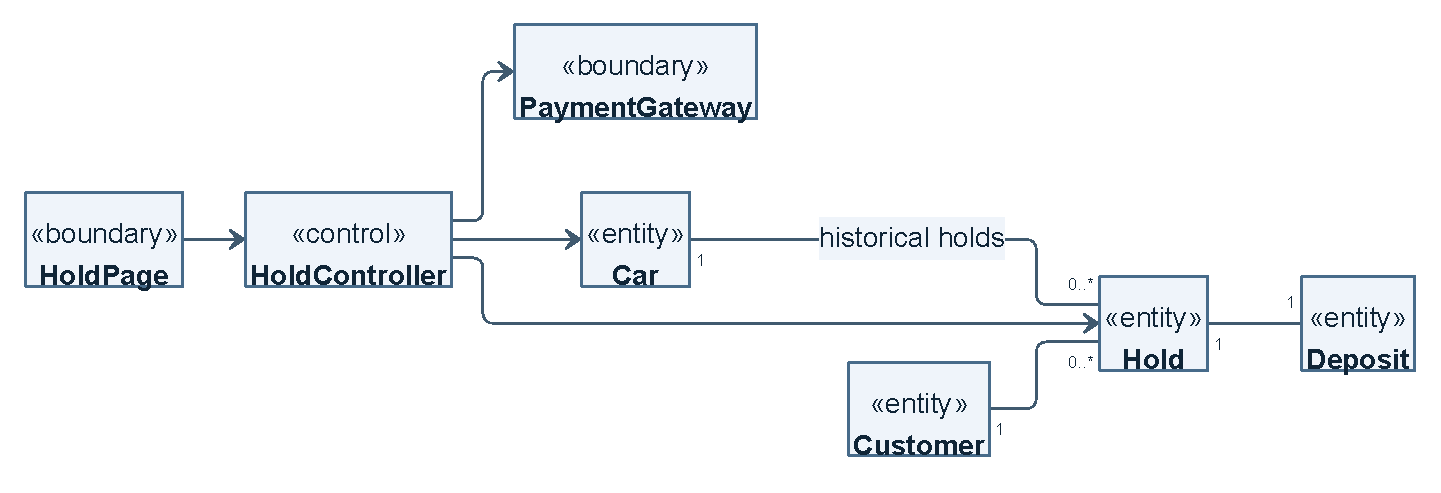
\includegraphics[width=405.68pt]{images/fig-049.pdf}
\captionof{figure}{Car sales: Q2 --- Analysis and process (25 marks)}\end{minipage}\par\smallskip



Constraint: each Car has \textbf{at most one active Hold}, even though historical holds are many. Customer may have multiple holds on different cars; Appendix A does not prohibit that. Attributes/\allowbreak{}operations are deliberately omitted for this analysis question.

\textbf{(b)} The hold dialog models screens, not physical car states.




\par\smallskip\noindent\begin{minipage}{\linewidth}\centering
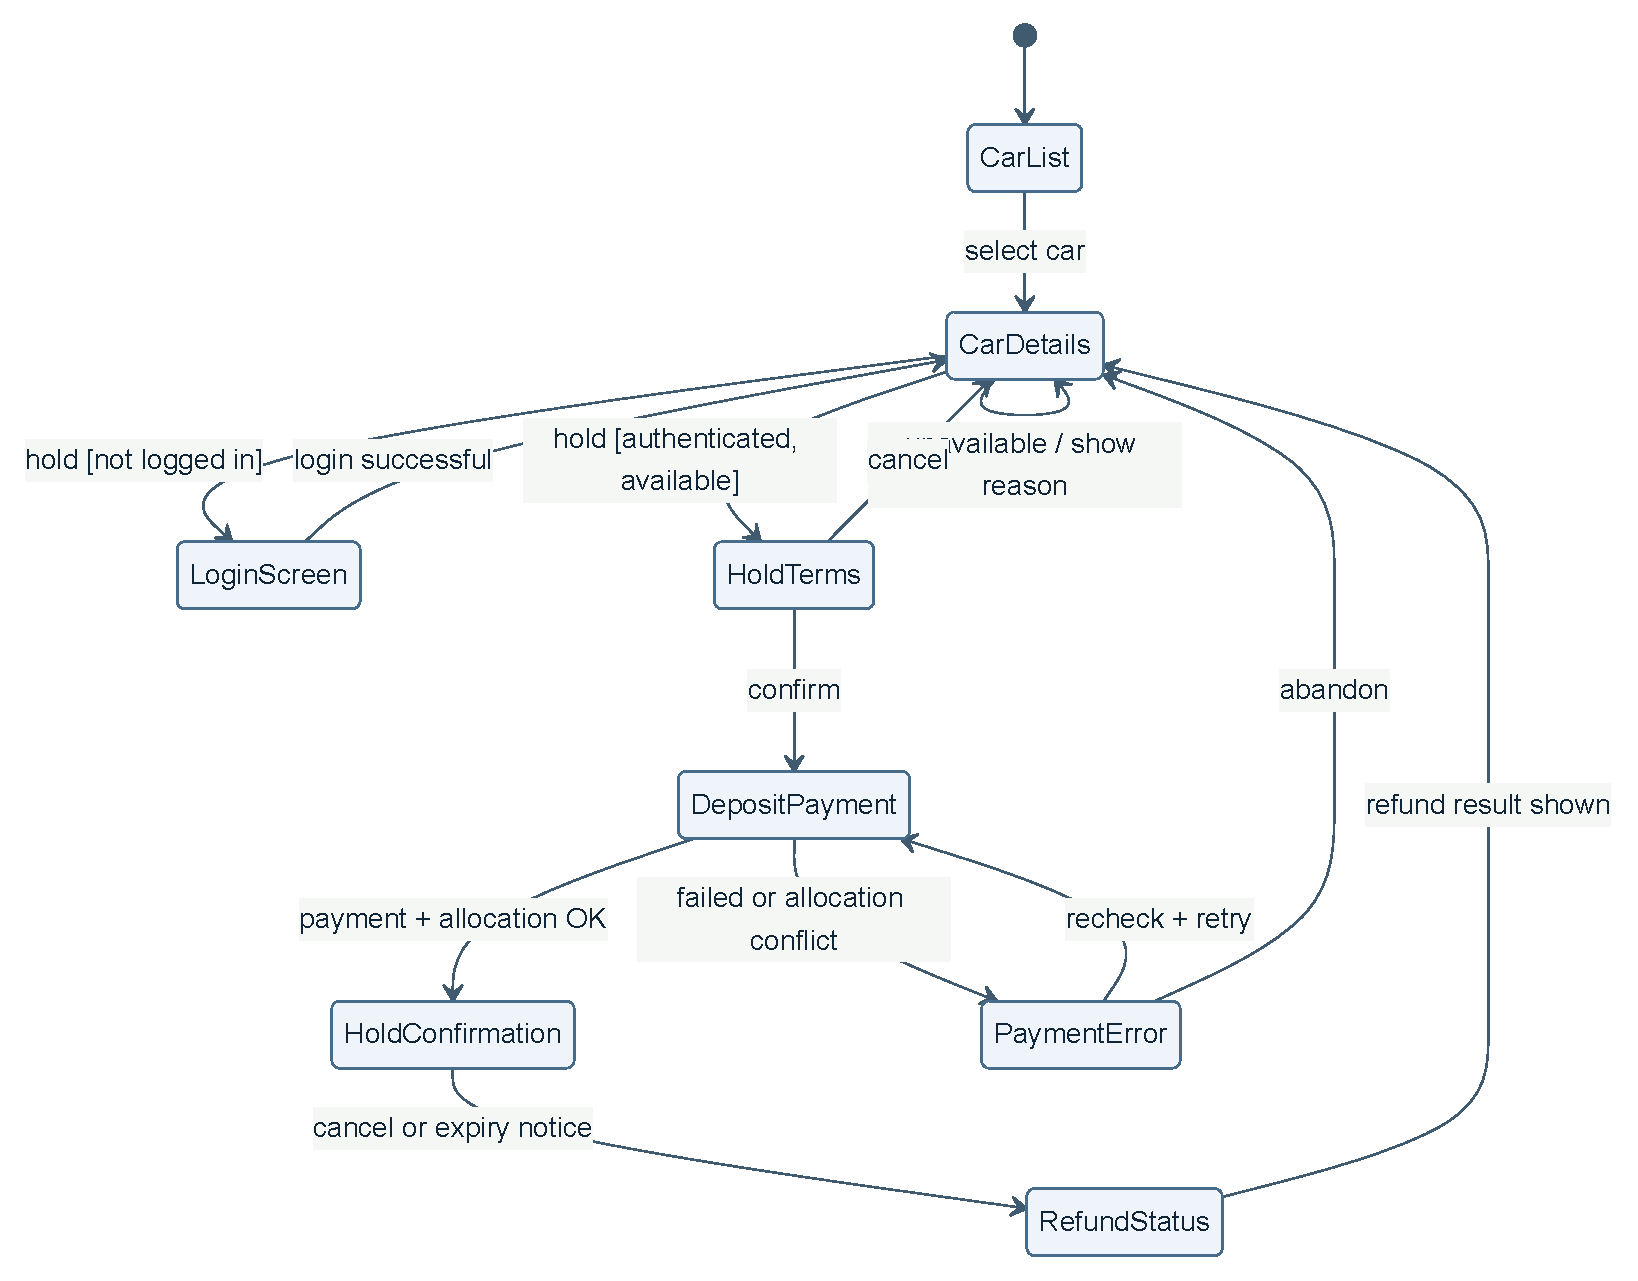
\includegraphics[width=461.12pt]{images/fig-050.pdf}
\captionof{figure}{Car sales: Q2 --- Analysis and process (25 marks)}\end{minipage}\par\smallskip



Terms/\allowbreak{}error/\allowbreak{}refund screens are proposed interface details. The business invariants from Q1 still apply.

\textbf{(c)} Use \hyperref[answer-waterfall]{W, p.\ \pageref{answer-waterfall}}: customer reviews expose change early; agreed downstream impact/replanning is still necessary.

\textbf{(d)} Use \hyperref[answer-scrum]{S, p.\ \pageref{answer-scrum}}: track remaining effort/velocity with a burndown; forecast capacity and negotiate priorities as scope changes.
\par\Needspace{85pt}\subsection*{AY2022/23 S2: Shopping chatbot --- Q2 (25 marks)}\label{old-2223-s2-q2}

\sectionlabel{h-q2--analysis-and-development-process-25-marks}
\textbf{(a) Replacement conceptual classes with stereotypes (7). (b) Replacement activity with user/\allowbreak{}chatbot/\allowbreak{}existing-system participants (8). (c) Why reuse-based integration/\allowbreak{}configuration can force requirement compromises, and mitigation (4). (d) Scrum Master response to a bug threatening sprint completion (6).}


\textbf{(a)}




\par\smallskip\noindent\begin{minipage}{\linewidth}\centering
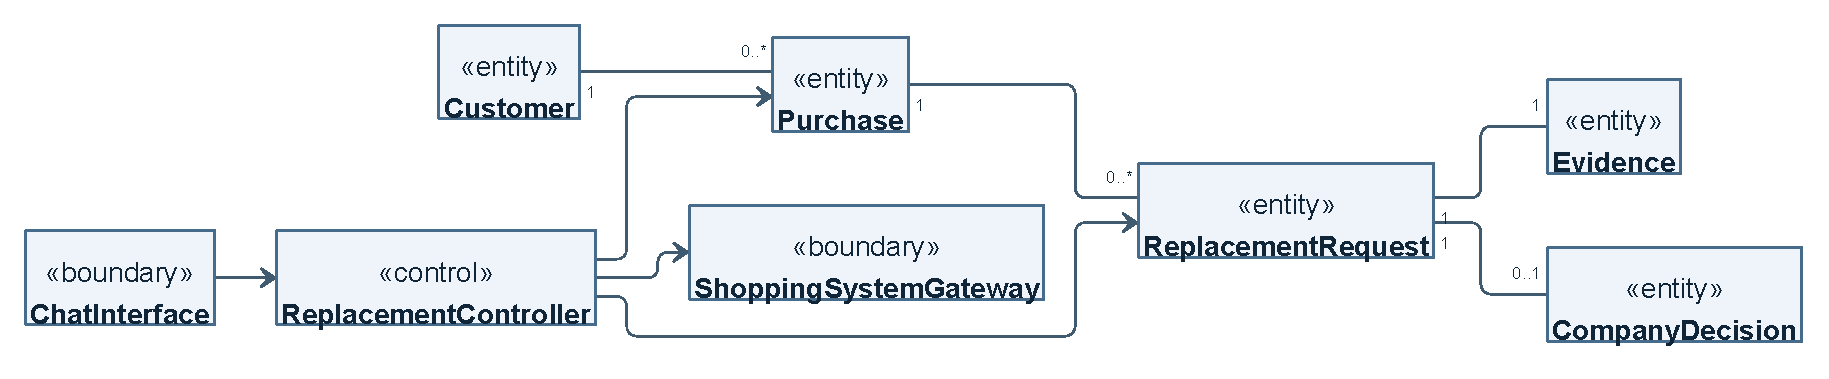
\includegraphics[width=514.00pt]{images/fig-054.pdf}
\captionof{figure}{Shopping chatbot: Q2 --- Analysis and development process (25 marks)}\end{minipage}\par\smallskip



Decision is absent while pending. Evidence groups photos, receipt and reason; its presence does not imply that an incomplete submission is approved.

\textbf{(b)} Subgraphs approximate activity swimlanes. Company approval is an activity of the existing system's organisation, not an autonomous chatbot decision.






\par\smallskip\noindent\begin{minipage}{\linewidth}\centering
{\scriptsize\textbf{Eligibility and evidence}}\par\smallskip
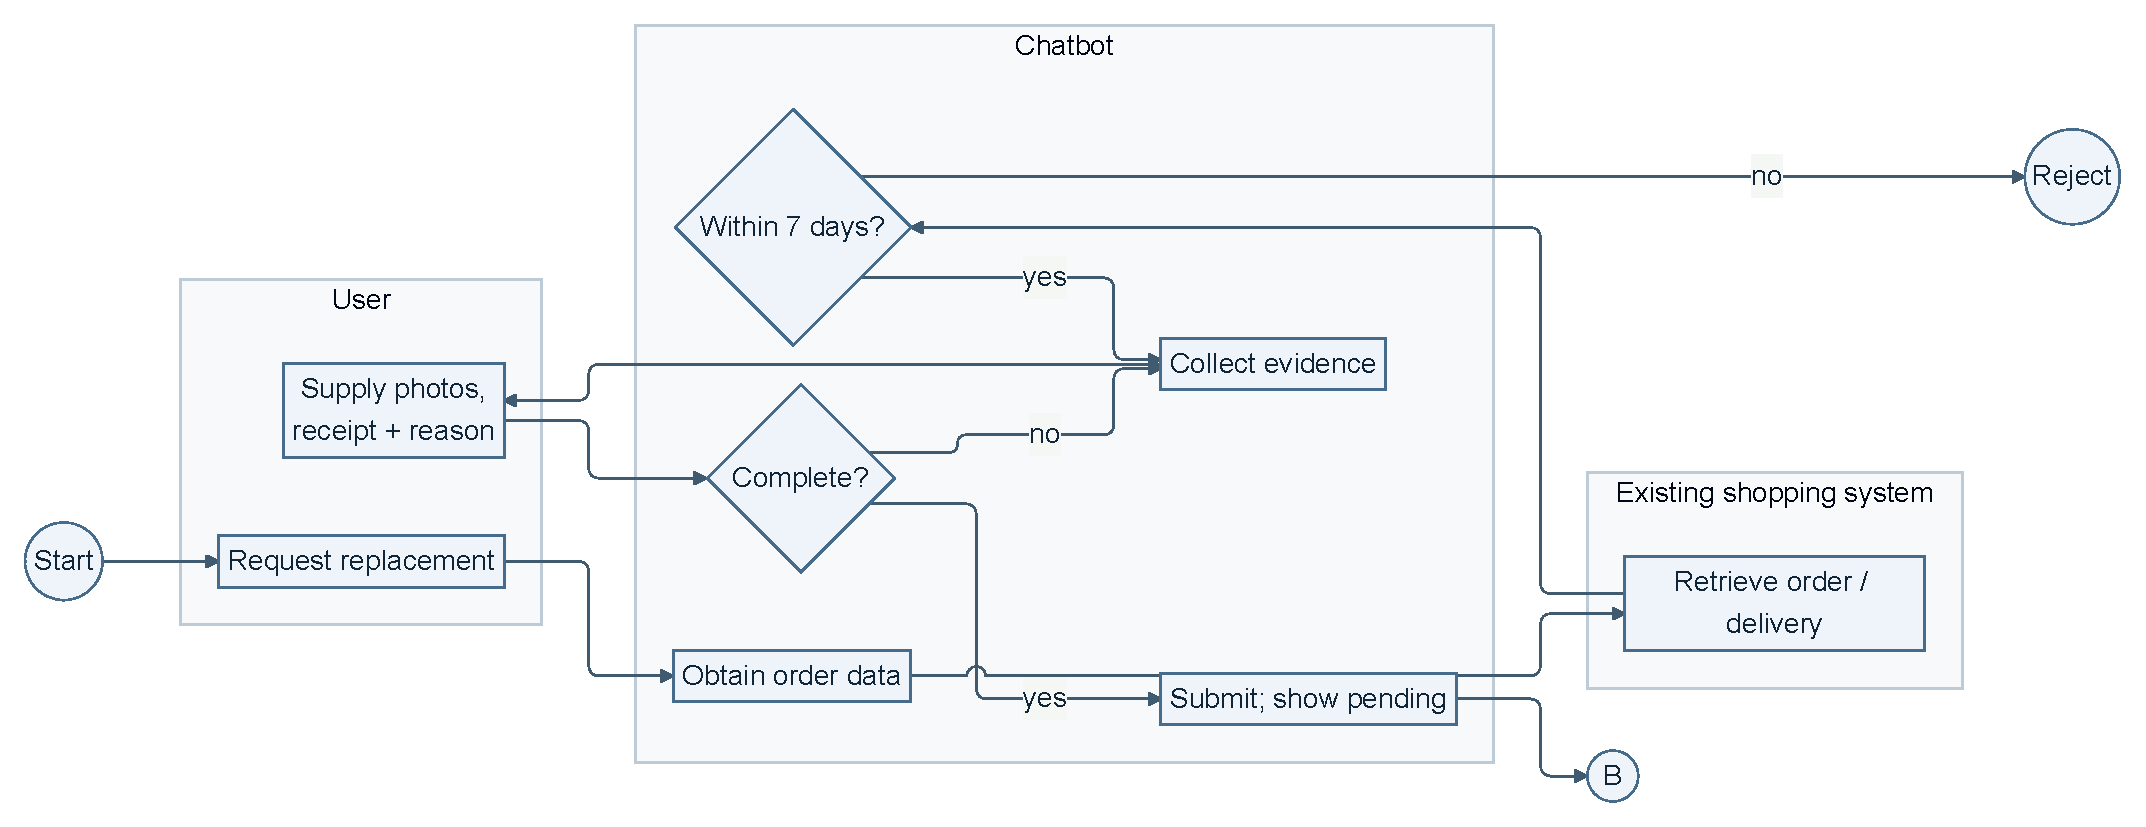
\includegraphics[width=514.00pt]{images/fig-055-a.pdf}\par\smallskip
{\scriptsize\textbf{Company decision and outcome}}\par\smallskip
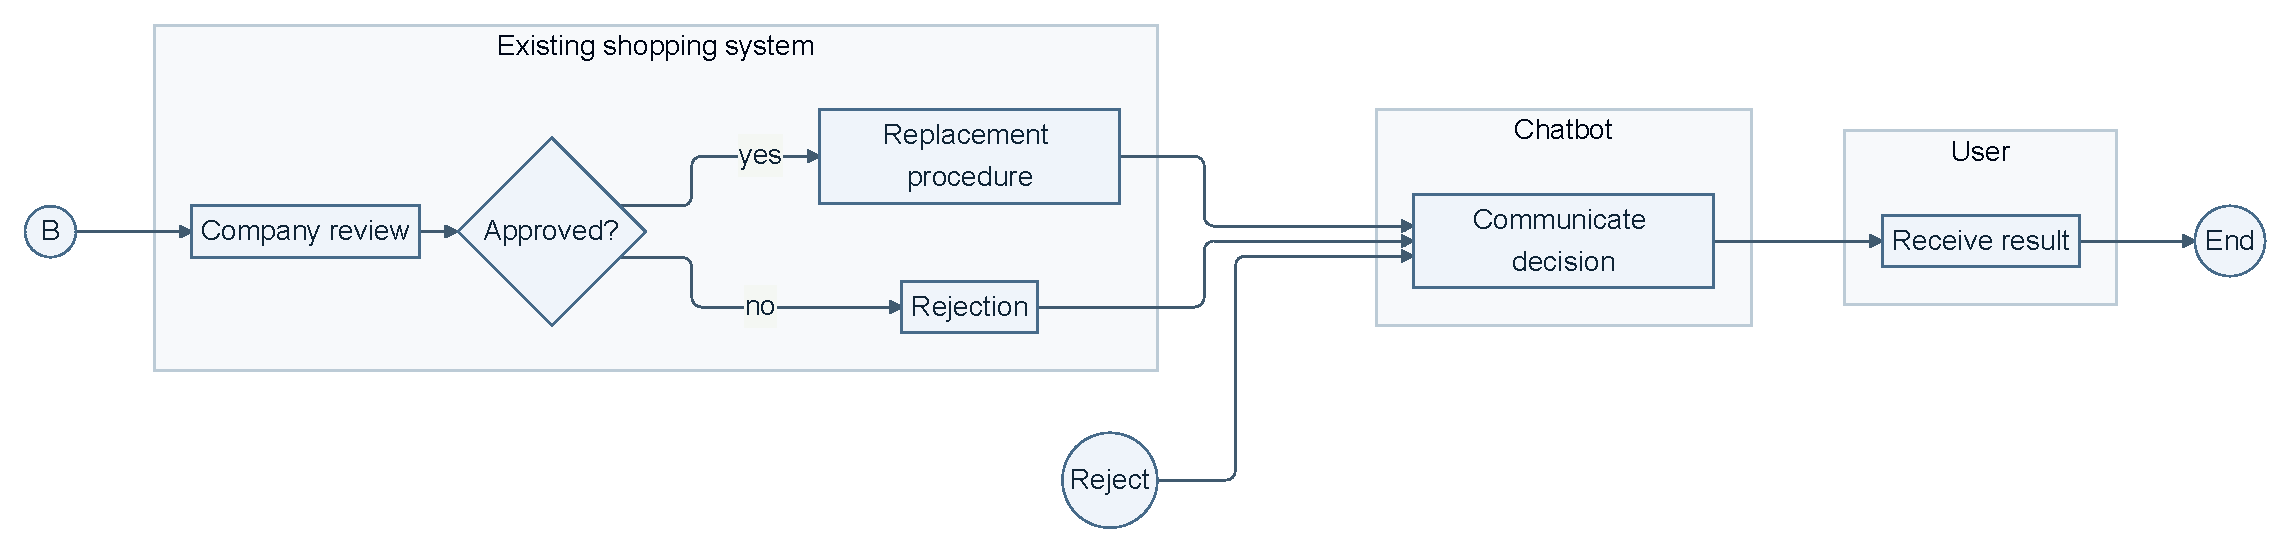
\includegraphics[width=514.00pt]{images/fig-055-b.pdf}\par\smallskip
\captionof{figure}{Shopping chatbot: Q2 --- Analysis and development process (25 marks)}\end{minipage}\par\smallskip









\textbf{(c)} Use \hyperref[answer-waterfall]{W, p.\ \pageref{answer-waterfall}} for reuse: compare the existing shop with must-have requirements, prototype its interfaces, negotiate acceptable compromises and adapt/build unmet essentials.

\textbf{(d)} Apply \hyperref[answer-scrum]{S, p.\ \pageref{answer-scrum}}: expose the bug, let developers investigate, assess Sprint Goal/severity, negotiate less essential work and review prevention. The Scrum Master facilitates.
\par\Needspace{85pt}\subsection*{AY2023/24 S1: DevSecOps --- Q2 (25 marks)}\label{old-2324-s1-q2}

\sectionlabel{h-q2--analysis-and-agile-25-marks}
\textbf{(a) Security-check conceptual classes/\allowbreak{}stereotypes (8). (b) Activity diagram with swimlanes (8). (c) Explain how incremental development can be plan-driven or agile (4). (d) Why may agile struggle with widely varying team skills? (5).}


\textbf{(a)}




\par\smallskip\noindent\begin{minipage}{\linewidth}\centering
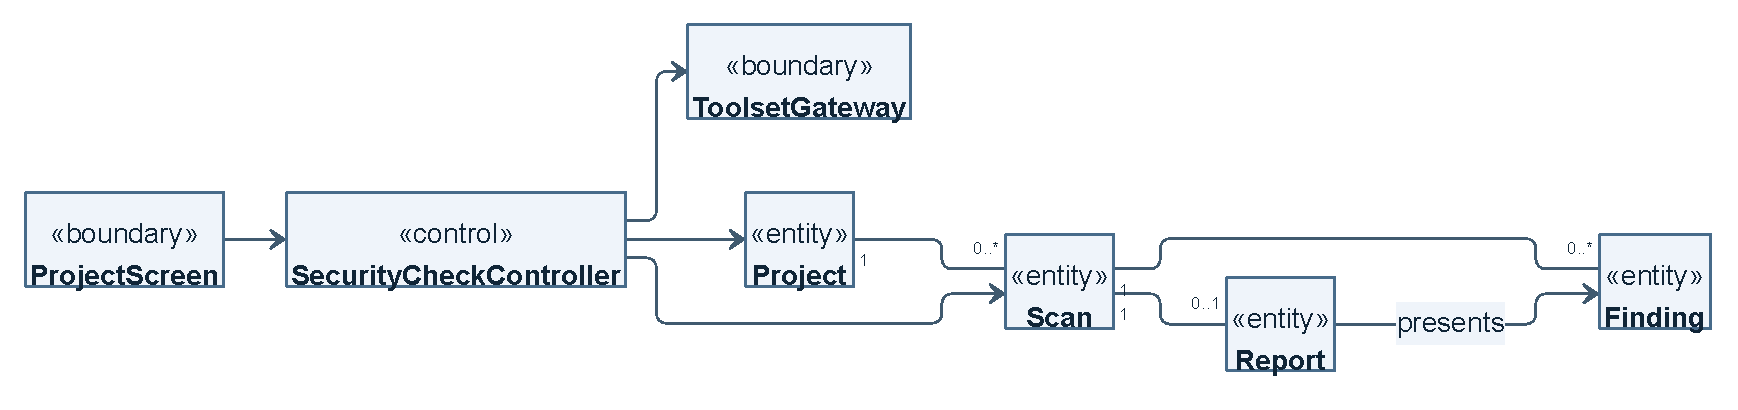
\includegraphics[width=488.84pt]{images/fig-059.pdf}
\captionof{figure}{DevSecOps: Q2 --- Analysis and agile (25 marks)}\end{minipage}\par\smallskip



\textbf{(b)} The external tool lane represents selected engines, not people inside the platform. Activities may be scheduled in parallel if dependencies permit; that scheduling is not specified by Appendix A.






\par\smallskip\noindent\begin{minipage}{\linewidth}\centering
{\scriptsize\textbf{A: scan and report}}\par\smallskip
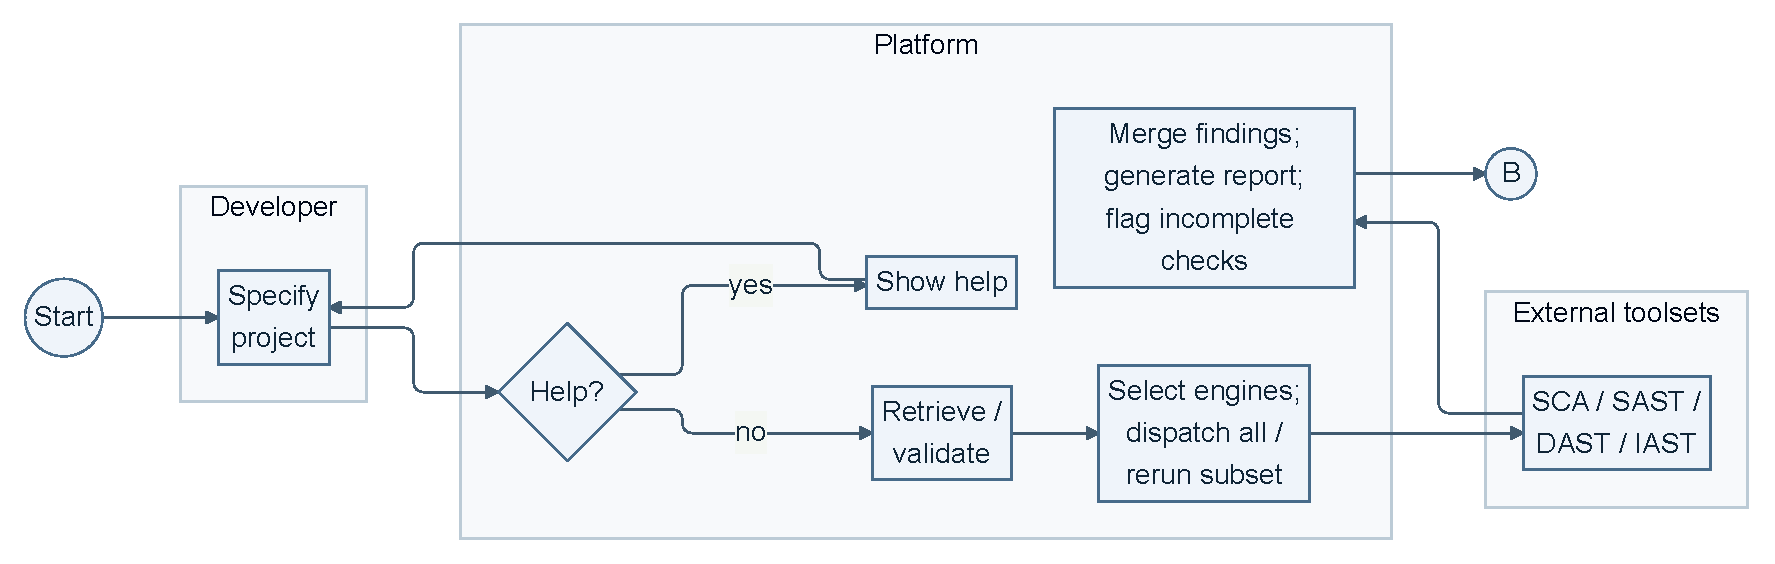
\includegraphics[width=454.00pt]{images/fig-060-a.pdf}\par\smallskip
{\scriptsize\textbf{B: review, mitigation and selected rerun}}\par\smallskip
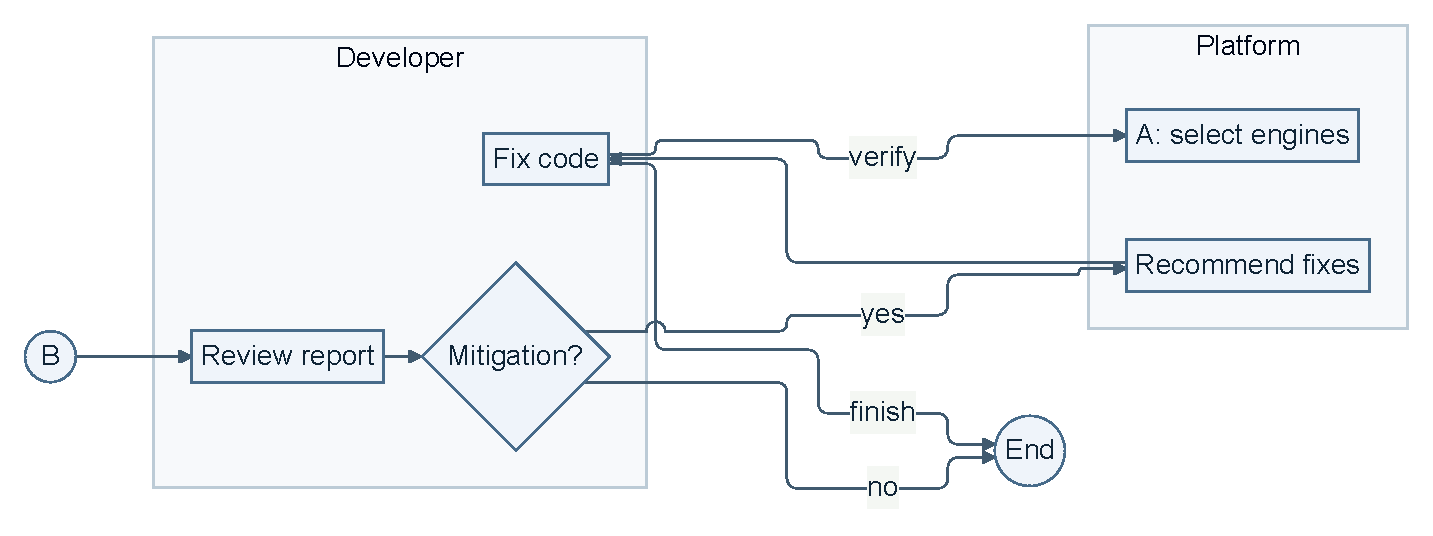
\includegraphics[width=366.80pt]{images/fig-060-b.pdf}\par\smallskip
\captionof{figure}{DevSecOps: DevSecOps activity workflow --- combined scan/report and review/rerun phases; B continues below, A returns to engine selection.}\end{minipage}\par\smallskip










\textbf{(c)} Use \hyperref[answer-waterfall]{W, p.\ \pageref{answer-waterfall}}: increments may be preplanned or reprioritised through feedback; delivery structure alone does not establish agile management.

\textbf{(d)} Use \hyperref[answer-scrum]{S, p.\ \pageref{answer-scrum}}: uneven skills risk quality, estimates, expert bottlenecks and integration. Pair/mentor, standardise and automate tests; diversity itself is not disqualifying.
\par\Needspace{85pt}\subsection*{AY2023/24 S2: CodeAgent --- Q2 (25 marks)}\label{old-2324-s2-q2}

\sectionlabel{h-q2--reviewer-analysis-qa-states-and-process-25-marks}
\textbf{(a) Reviewer conceptual classes/\allowbreak{}stereotypes (9). (b) QA-Checker state machine (7). (c) Two ways plan-driven projects can handle changing requirements (4). (d) Importance of Scrum velocity (5).}


\textbf{(a)}




\par\smallskip\noindent\begin{minipage}{\linewidth}\centering
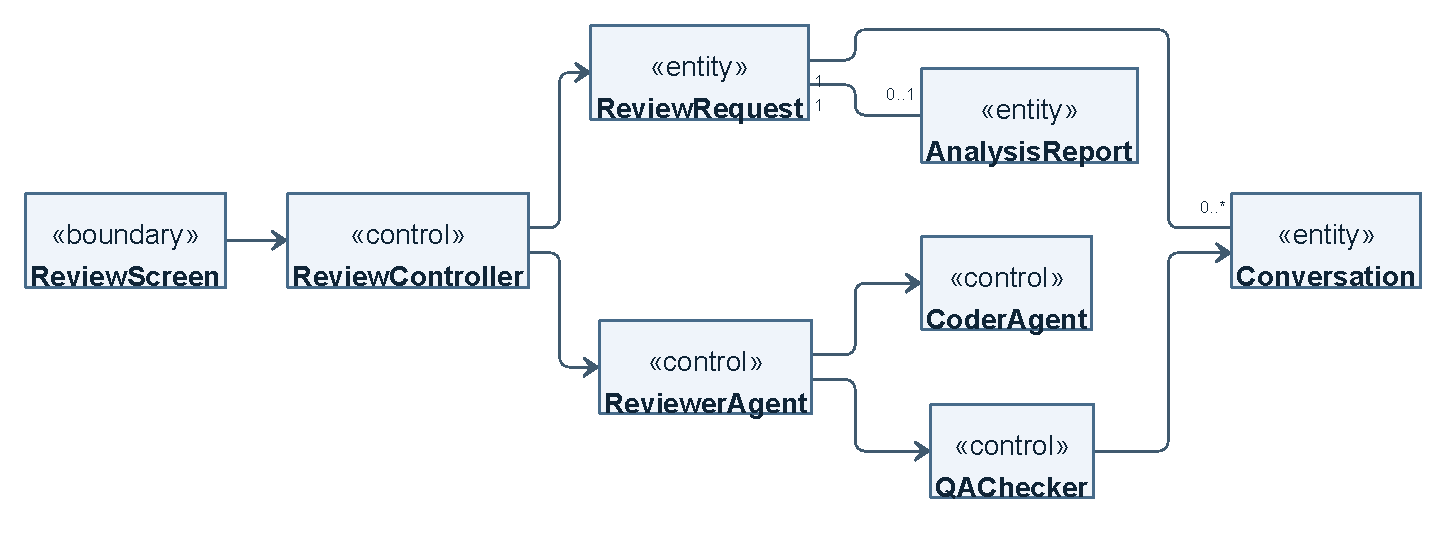
\includegraphics[width=407.44pt]{images/fig-065.pdf}
\captionof{figure}{CodeAgent: Q2 --- Reviewer analysis, QA states and process (25 marks)}\end{minipage}\par\smallskip



Agents coordinate behaviour; they are not merely stored domain records. ReviewRequest groups commit, message and original files. Report is absent before completion; unresolved status is possible.

\textbf{(b)} Let \code{n} count answers received and \code{max} be the configured maximum dialogue count. Assume \code{max \ensuremath{\geq} 1}. On the first received answer set \code{n=\allowbreak{}1}.




\par\smallskip\noindent\begin{minipage}{\linewidth}\centering
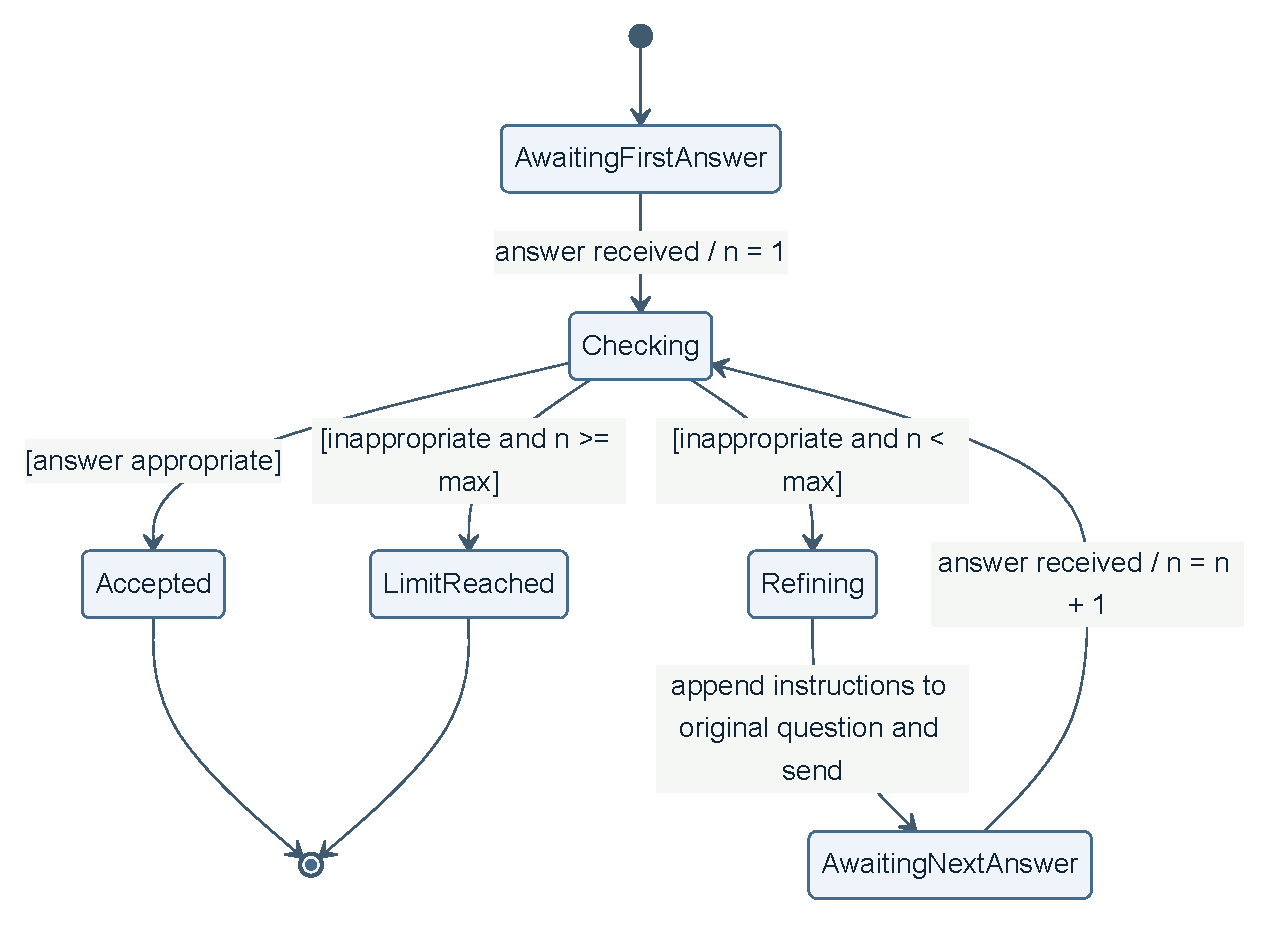
\includegraphics[width=357.72pt]{images/fig-066.pdf}
\captionof{figure}{CodeAgent: Q2 --- Reviewer analysis, QA states and process (25 marks)}\end{minipage}\par\smallskip

\begin{studycolumns}
\vspace{0pt}



Accept an appropriate answer even on the last permitted round. LimitReached means unresolved, not accepted. This models supervision of \textbf{one conversation}; a new conversation starts a new instance/\allowbreak{}reset.

\textbf{(c)} Apply \hyperref[answer-waterfall]{W, p.\ \pageref{answer-waterfall}} with two measures: early prototypes/reviews or planned increments; approved change control updating affected baselines, schedule, budget and tests.

\textbf{(d)} Use \hyperref[answer-scrum]{S, p.\ \pageref{answer-scrum}}: completed velocity supports feasible sprint selection and remaining-effort forecasts. Reforecast capacity; exclude unfinished work and inflated estimates.
\end{studycolumns}


\fontsize{9}{10.5}\selectfont
\par\Needspace{100pt}\section*{Older Q3: Architecture, NFRs and patterns}\label{older-q3}
\phantomsection\addcontentsline{toc}{section}{Older Q3: Architecture, NFRs and patterns}
\markboth{Older papers | Q3}{}
\textbf{Shared method:} use \hyperref[answer-architecture]{A, p.\ \pageref{answer-architecture}}, \hyperref[shared-pattern]{P, p.\ \pageref{shared-pattern}}, \hyperref[answer-mvc]{M, p.\ \pageref{answer-mvc}} and \hyperref[answer-pattern-cost]{C, p.\ \pageref{answer-pattern-cost}}. The case answers supply the concrete responsibilities, constraints and trade-offs.
\par\Needspace{85pt}\subsection*{AY2022/23 S1: Car sales --- Q3 (25 marks)}\label{old-2223-s1-q3}

\sectionlabel{h-q3--architecture-and-pattern-composition-25-marks}
\textbf{(a)(i) Architecture and detailed classes (8); (ii) alternative using a different pattern and its advantages (6). (b)(i) Combined-pattern car-sales scenario and classes (8); (ii) when patterns can be combined/\allowbreak{}merged, with an example (3).}


\textbf{(a)(i)} Apply the shared layered frame. HoldController enforces allocation/\allowbreak{}refund rules rather than putting them into the page. Extend Q2's conceptual model as follows:







\par\smallskip\noindent\begin{minipage}{\linewidth}\centering
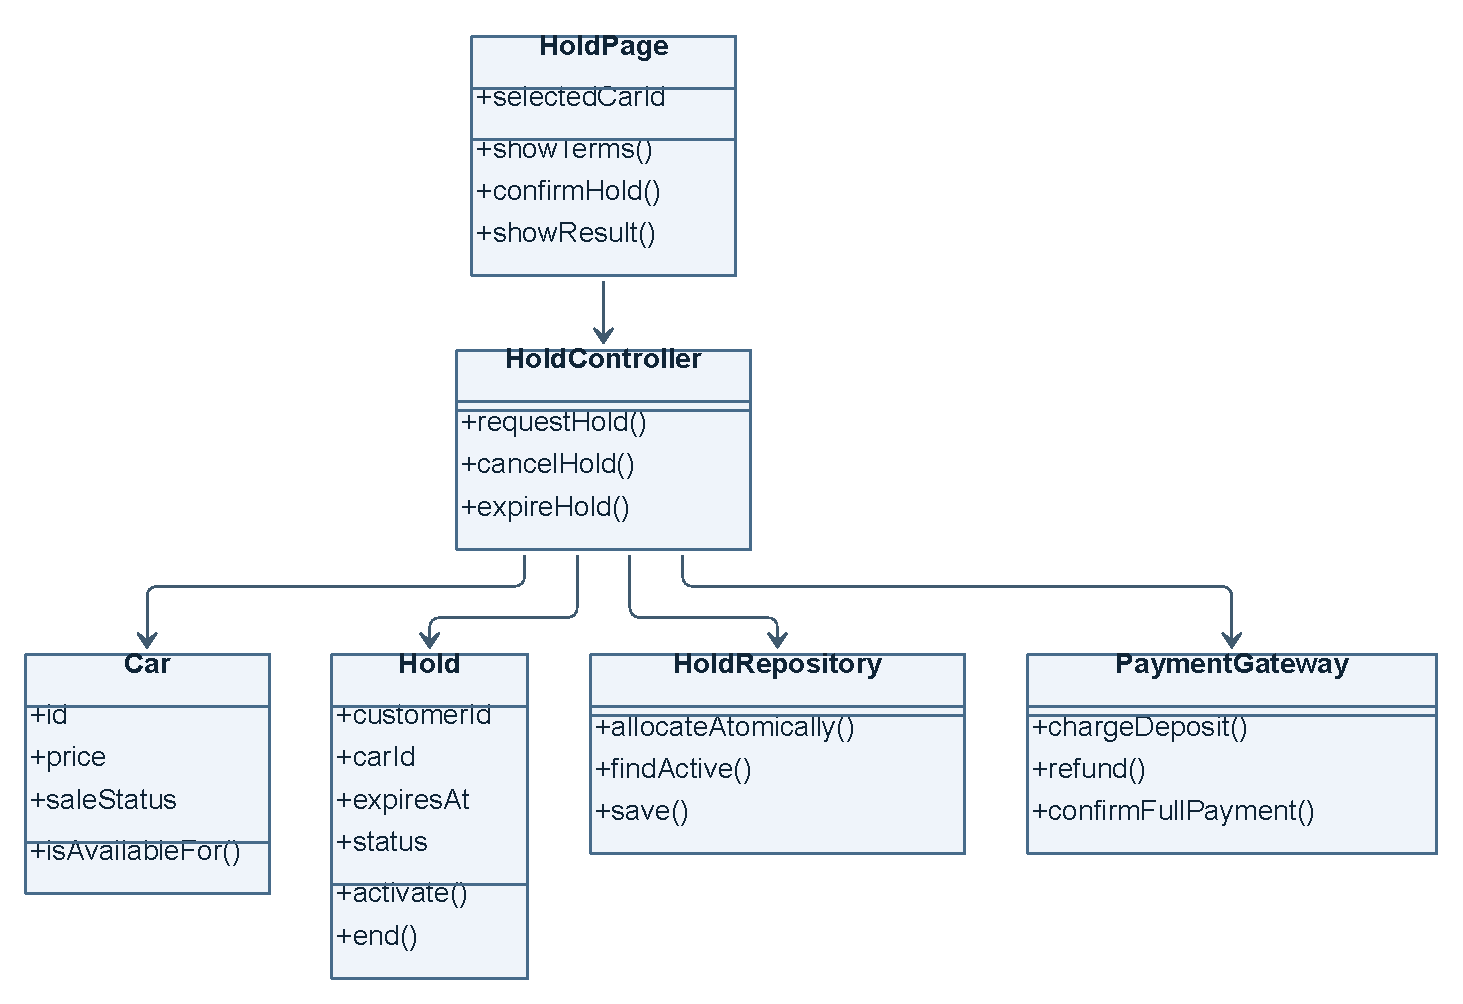
\includegraphics[width=408.22pt]{images/fig-051.pdf}
\captionof{figure}{Car sales: Q3 --- Architecture and pattern composition (25 marks)}\end{minipage}\par\smallskip

\begin{studycolumns}
\vspace{0pt}





Order/\allowbreak{}delivery controls similarly require full-payment confirmation before delivery. Persistence must enforce active-hold uniqueness; payment callbacks need reconciliation to avoid recording inconsistent states.

\textbf{(a)(ii)} Apply \hyperref[answer-mvc]{M, p.\ \pageref{answer-mvc}}. Model: Car/Hold plus services; Views: listing/details/status screens; Controller: HoldController. Notify both staff and customers when hold state changes; layered persistence can remain.

\textbf{(b)(i)} Combine \textbf{Strategy} with \textbf{Simple Factory} for selecting a dealer payment provider. This is a proposed extension; the appendix only requires integration with the dealer payment system.


\textbf{Class diagram:} use \hyperref[shared-pattern]{P, p.\ \pageref{shared-pattern}}. Context = \code{Hold\allowbreak{}Controller}; Strategy = \code{Payment\allowbreak{}Strategy}; Factory = \code{Payment\allowbreak{}Factory}. Concrete strategies: \code{Card\allowbreak{}Payment}, \code{Wallet\allowbreak{}Payment}. Interface/concrete operations: \code{charge()}, \code{refund()}. Provider selection is a proposed extension; retain availability, allocation and refund rules.



Patterns do not replace validation or transaction handling.

\textbf{(b)(ii)} Use \hyperref[answer-pattern-cost]{C, p.\ \pageref{answer-pattern-cost}}. MVC combines Observer/Strategy; the payment example separates behaviour from construction. Shared classes are acceptable when responsibilities stay clear.
\end{studycolumns}

\par\Needspace{85pt}\subsection*{AY2022/23 S2: Shopping chatbot --- Q3 (25 marks)}\label{old-2223-s2-q3}

\sectionlabel{h-q3--chatbot-architecture-and-combined-patterns-25-marks}
\textbf{(a)(i) Architecture/\allowbreak{}detailed classes (8); (ii) alternative pattern and advantages (6). (b)(i) Combined patterns and class diagram (8); (ii) structural method for comparing architectures (3).}


\textbf{(a)(i)} Apply the shared layered frame with a gateway to the existing shop. Keep order/\allowbreak{}replacement decisions in deterministic services; natural-language interpretation identifies the requested operation.




\par\smallskip\noindent\begin{minipage}{\linewidth}\centering
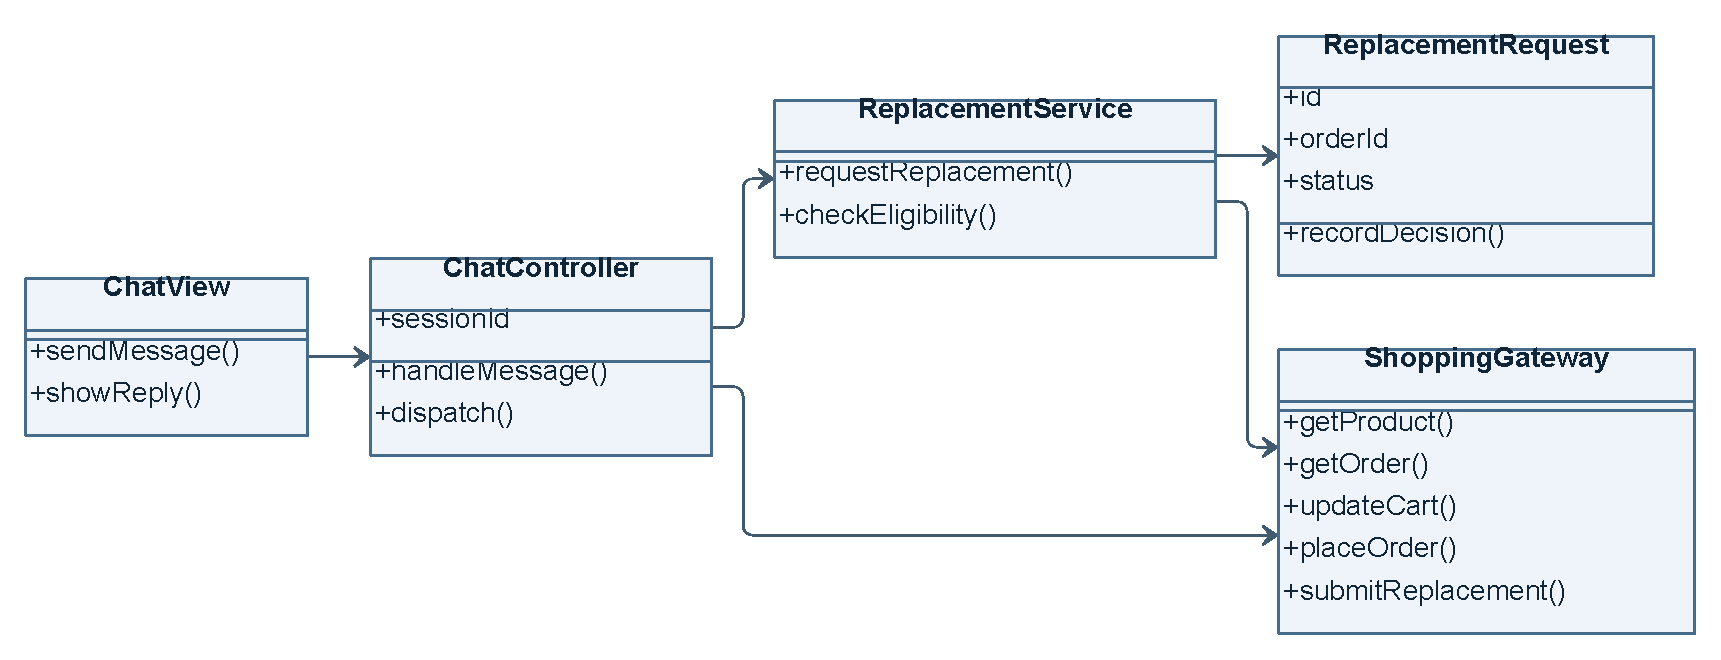
\includegraphics[width=484.44pt]{images/fig-056.pdf}
\captionof{figure}{Shopping chatbot: Q3 --- Chatbot architecture and combined patterns (25 marks)}\end{minipage}\par\smallskip

\begin{studycolumns}
\vspace{0pt}



\textbf{(a)(ii)} Apply \hyperref[answer-mvc]{M, p.\ \pageref{answer-mvc}}. Models: conversation/cart/replacement request; Views: chat and order status; Controllers: input handling. Notify both views when the company decision arrives; retain layered services underneath.

\textbf{(b)(i)} Combine Strategy for handling different intents with Simple Factory for selecting the handler:


\textbf{Class diagram:} use \hyperref[shared-pattern]{P, p.\ \pageref{shared-pattern}}. Context = \code{Chat\allowbreak{}Controller}; Strategy = \code{Intent\allowbreak{}Handler}; Factory = \code{Handler\allowbreak{}Factory}. Concrete strategies: \code{Product\allowbreak{}Query\allowbreak{}Handler}, \code{Replacement\allowbreak{}Handler}, \code{Refund\allowbreak{}Handler}. Interface/concrete operations: \code{execute()}. The chatbot selects behaviour; the existing shop still makes the company approval decision.





\textbf{(b)(ii)} Use \hyperref[answer-architecture]{A, p.\ \pageref{answer-architecture}}: compare cohesion, coupling, cycles and change propagation. A changed shopping API should affect its gateway, not every handler/view; raw class/edge counts alone prove little.
\end{studycolumns}

\par\Needspace{85pt}\subsection*{AY2023/24 S1: DevSecOps --- Q3 (25 marks)}\label{old-2324-s1-q3}


\begin{studycolumns}
\vspace{0pt}
\sectionlabel{h-q3--quality-attributes-and-architecture-25-marks}
\textbf{(a)(i) Important NFRs (6); (ii) detailed architecture/\allowbreak{}classes addressing them (8). (b)(i) Combined-pattern scenario/\allowbreak{}classes (6); (ii) can AI design software architectures? (5).}


\textbf{(a)(i)} Apply \hyperref[answer-architecture]{A, p.\ \pageref{answer-architecture}} to three proposed NFRs: source confidentiality/isolated execution; replaceable interoperable engines; responsive, reliable long-running scans. Agree measurable criteria rather than inventing guaranteed numbers.

\textbf{(a)(ii)} Add plug-in engine boundaries to the shared layered frame. A scan coordinator implements a Facade for the UI; a stable Engine interface supports replacement tool adapters. Proposed queued jobs and isolated execution address responsiveness and fault containment.
\end{studycolumns}


\par\smallskip\noindent\begin{minipage}{\linewidth}\centering
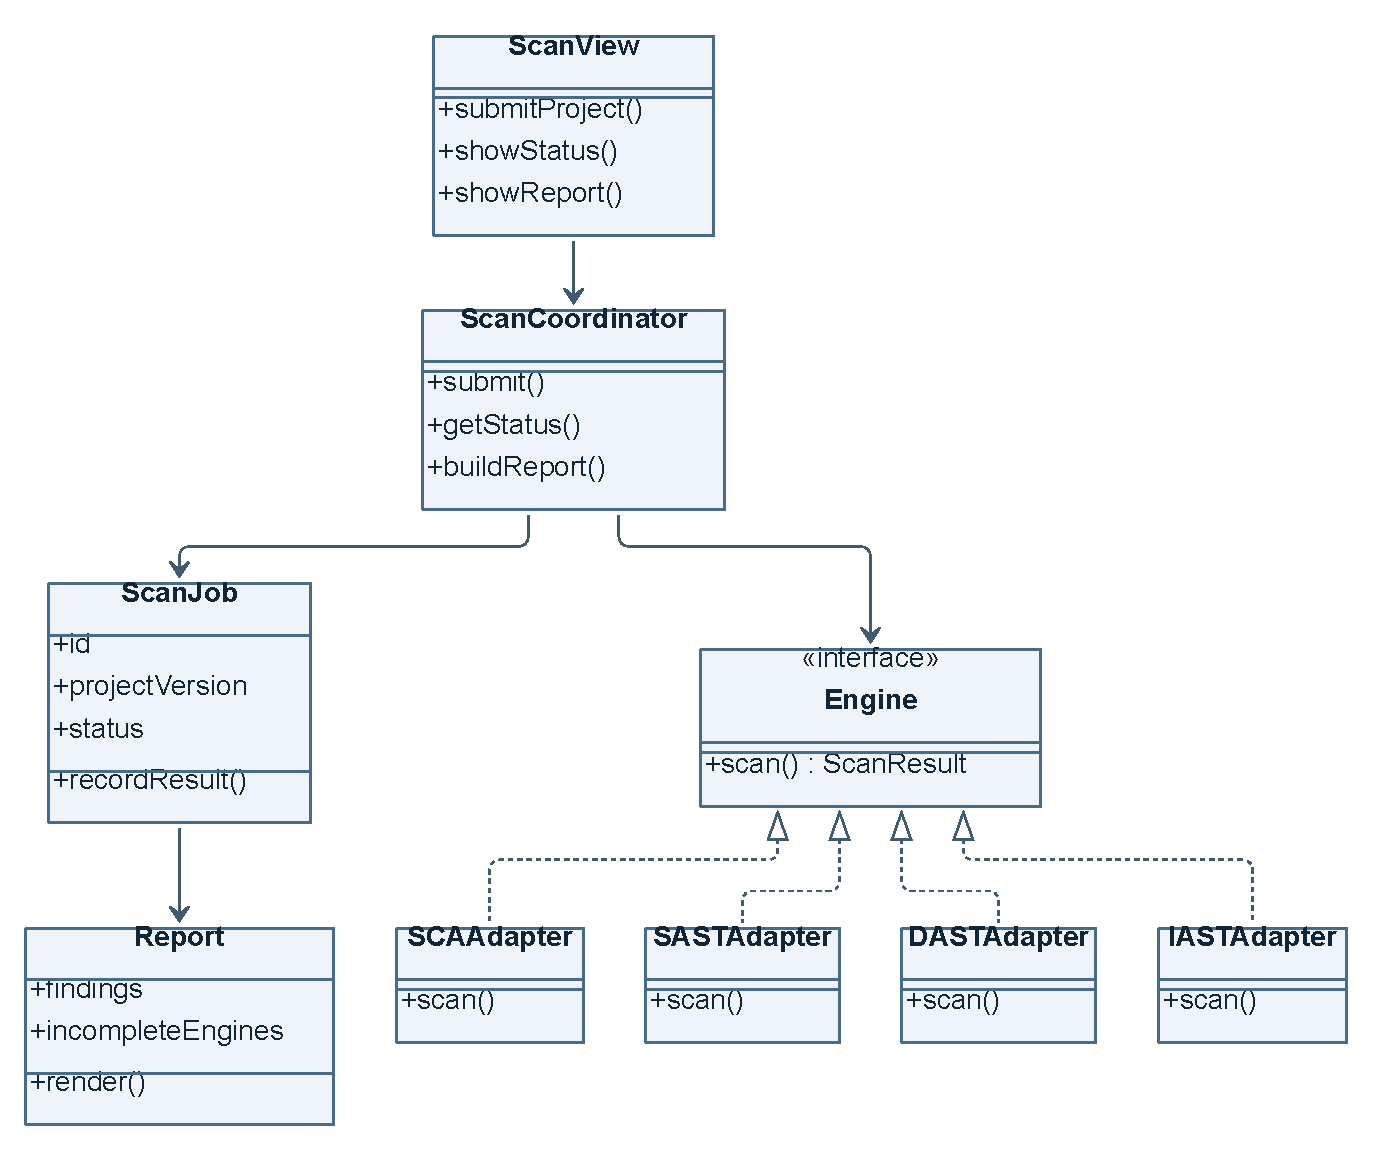
\includegraphics[width=386.32pt]{images/fig-061.pdf}
\captionof{figure}{DevSecOps: Q3 --- Quality attributes and architecture (25 marks)}\end{minipage}\par\smallskip

\begin{studycolumns}
\vspace{0pt}




Isolate source access and credentials at adapter/\allowbreak{}execution boundaries; apply timeouts and preserve partial-failure information. Adding an engine should add an adapter rather than change UI or report-domain rules. These choices directly connect the architecture to the proposed NFRs.

\textbf{(b)(i)} Combine Strategy and Simple Factory: engines share the Engine contract while an EngineFactory creates configured adapters. ScanCoordinator uses the resulting strategies without knowing their concrete classes.


\textbf{Class diagram:} use \hyperref[shared-pattern]{P, p.\ \pageref{shared-pattern}}. Context = \code{Scan\allowbreak{}Coordinator}; Strategy = \code{Engine}; Factory = \code{Engine\allowbreak{}Factory}. Concrete strategies: \code{SASTAdapter}, \code{SCAAdapter}, \code{DASTAdapter}, \code{IASTAdapter}. Interface/concrete operations: \code{scan()}. Create configured tool adapters; preserve the engine result/partial-failure contract.





\textbf{(b)(ii)} AI can propose candidate NFRs, architectures, diagrams and trade-offs. It cannot set missing stakeholder priorities or prove security/performance/integration fitness. Ground it in requirements, review traceability and validate risky decisions with prototypes/tests and human judgement.
\end{studycolumns}

\par\Needspace{85pt}\subsection*{AY2023/24 S2: CodeAgent --- Q3 (25 marks)}\label{old-2324-s2-q3}


\begin{studycolumns}
\vspace{0pt}
\sectionlabel{h-q3--extending-codeagent-and-architecture-25-marks}
\textbf{(a)(i) Two additional agent roles (3); (ii) one important NFR (3); (iii) detailed architecture addressing it (8). (b)(i) Combined-pattern scenario/\allowbreak{}classes (6); (ii) can CodeAgent replace development teams? (5).}


\textbf{(a)(i)} A \textbf{Test Engineer agent} creates/\allowbreak{}executes candidate regression tests and reports evidence; a \textbf{Requirements Analyst agent} clarifies requests and checks traceability between requirements and reviewed changes. These are proposed additions, distinct from the existing conversation-focused QA-Checker.

\textbf{(a)(ii)} Choose \textbf{extensibility/\allowbreak{}maintainability}: new agent roles and analysis strategies should be addable without changing all existing agents. The request to introduce roles makes this a defensible priority; correctness/\allowbreak{}security would also require attention in a real platform.

\textbf{(a)(iii)} Use layered UI/\allowbreak{}orchestration/\allowbreak{}domain boundaries with plug-in agents. A coordinator schedules phases and supervised conversations; agents implement a common contract; configuration/\allowbreak{}registry selects roles. This avoids hard-coded peer dependencies throughout the UI.
\end{studycolumns}


\par\smallskip\noindent\begin{minipage}{\linewidth}\centering
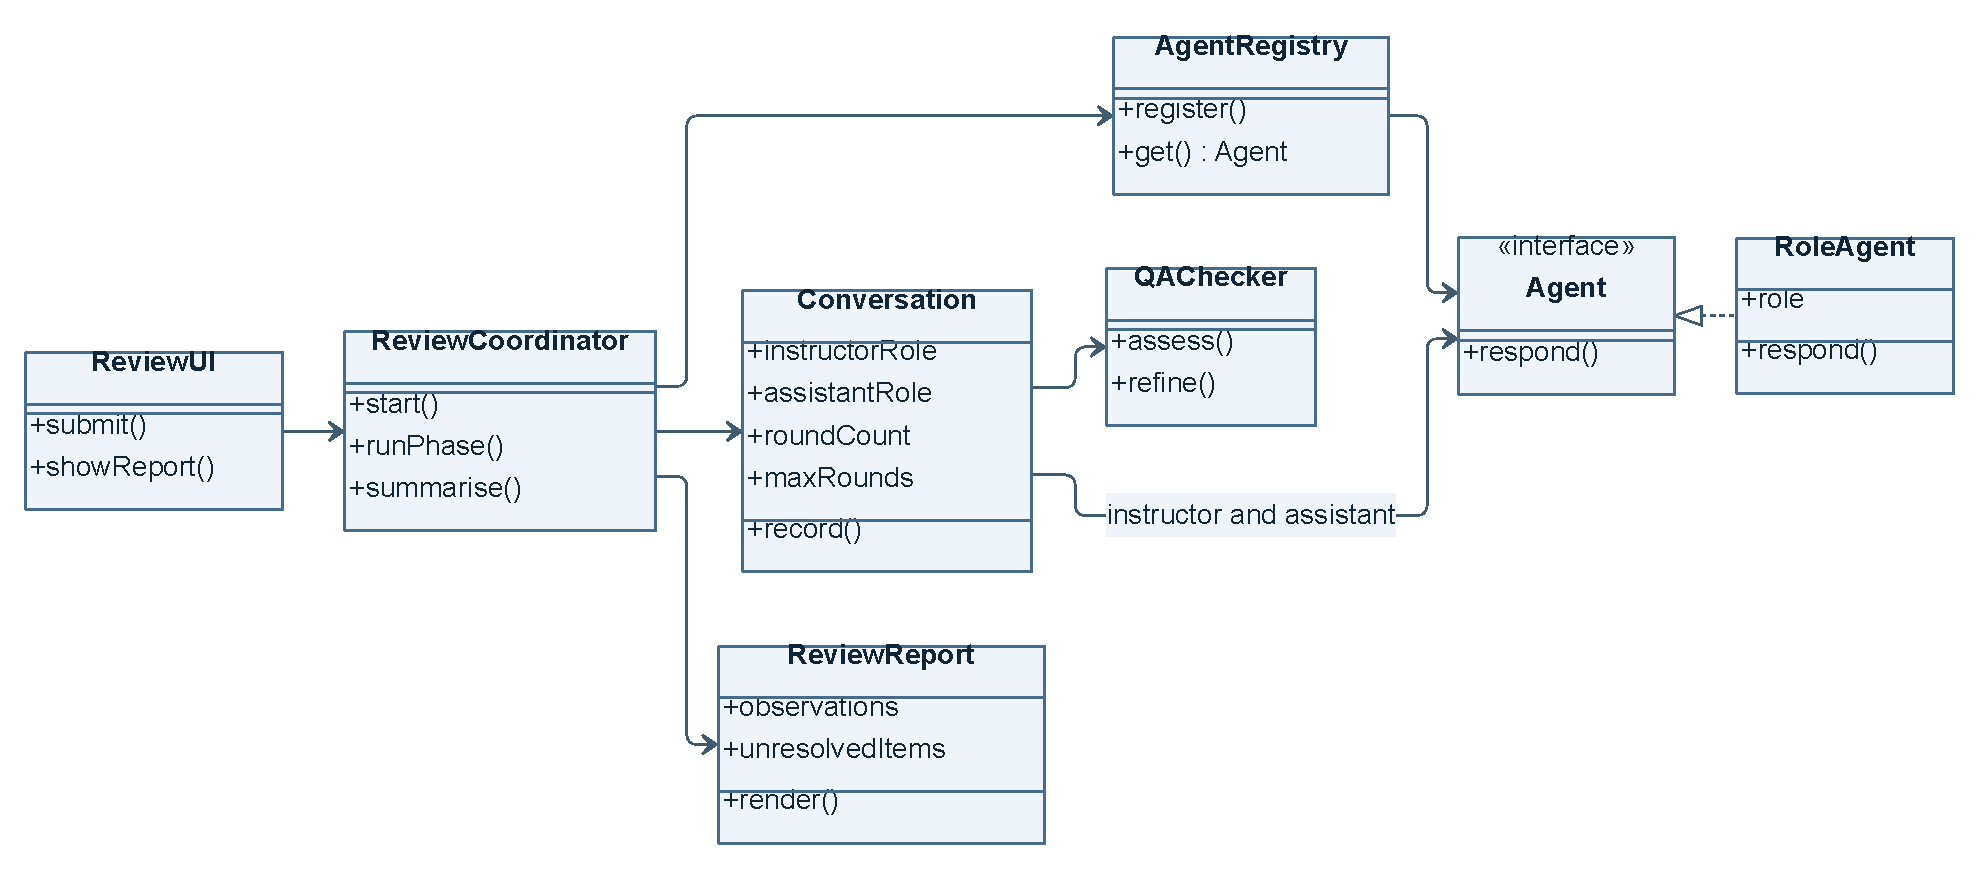
\includegraphics[width=514.00pt]{images/fig-067.pdf}
\captionof{figure}{CodeAgent: Q3 --- Extending CodeAgent and architecture (25 marks)}\end{minipage}\par\smallskip

\begin{studycolumns}
\vspace{0pt}



Configure RoleAgent for User/\allowbreak{}CEO/\allowbreak{}CPO/\allowbreak{}CTO/\allowbreak{}Reviewer/\allowbreak{}Coder, or add new Agent implementations. Persist logs and preserve unresolved status when conversation limits are reached. The registry approach supports the chosen extensibility NFR; storage and orchestration should not depend on one concrete role.

\textbf{(b)(i)} Combine Strategy for analysis methods with Simple Factory for constructing the requested checks:


\textbf{Class diagram:} use \hyperref[shared-pattern]{P, p.\ \pageref{shared-pattern}}. Context = \code{Reviewer\allowbreak{}Agent}; Strategy = \code{Review\allowbreak{}Check}; Factory = \code{Check\allowbreak{}Factory}. Concrete strategies: \code{Consistency\allowbreak{}Check}, \code{Vulnerability\allowbreak{}Check}, \code{Format\allowbreak{}Check}. Interface/concrete operations: \code{analyse()}. Choose the requested review check without hard-coding it in the reviewer.



Reviewer's three analyses retain separate responsibilities, while creation is centralised. A new check can be registered without duplicating the review workflow.

\textbf{(b)(ii)} CodeAgent assists review/revision, but does not replace stakeholder negotiation, requirements clarification, architecture judgement, independent validation, operations or accountability. Agent agreement is not proof of correct software; accept changes using reviewed outputs and executable tests.
\end{studycolumns}


\fontsize{9}{10.5}\selectfont
\par\Needspace{100pt}\section*{Older Q4: Input testing and applied testing/maintenance}\label{older-q4}
\phantomsection\addcontentsline{toc}{section}{Older Q4: Input testing and applied testing/maintenance}
\markboth{Older papers | Q4}{}
\begin{studycolumns}
\textbf{Shared input interpretation.} The older questions specify an ASCII identifier/description, a fixed-digit integer, a calendar-date range and an allowed category set. Assume positive numeric integers (leading zeroes do not count), inclusive complete years and one-day date resolution. Parsing policy is an explicit assumption; do not invent ASCII length, printable-only or nonempty restrictions.
\textbf{Shared EC/BV checks.} Each category set is one valid EC; testing all members adds coverage, not extra ECs. ASCII membership and unordered categories have no specified ordered application boundary. Malformed numbers/nonexistent dates are extra EC tests. Keep all boundary triplets and exactly one invalid field per defensive row. All original rows follow under their own cases.
\end{studycolumns}
\par\Needspace{85pt}\subsection*{AY2022/23 S1: Car sales --- Q4 (25 marks)}\label{old-2223-s1-q4}

\sectionlabel{h-q4--input-testing-test-levels-and-maintenance-25-marks}
\textbf{(a)(i) Derive ECs for Car Model, Price, Manufacturing Date and Color (4). (ii) Give on/\allowbreak{}below/\allowbreak{}above boundary values (4). (iii) Design defensive tests (5).}


\textbf{Input interpretation.} Car Model must be ASCII; Price is a 6-digit integer; Manufacturing Date is between 2010 and 2022; Color is one of \code{White}, \code{Black}, \code{Blue}, \code{Red}, \code{Others}. Apply the shared input interpretation above.

\textbf{(i) Equivalence classes:}




{\fontsize{8.5}{9.8}\selectfont
\begin{longtable}{L{\dimexpr 0.22341\linewidth-5.36pt\relax}L{\dimexpr 0.32885\linewidth-7.89pt\relax}L{\dimexpr 0.44775\linewidth-10.75pt\relax}}
\toprule
\rowcolor{ice}\textbf{Field} & \textbf{Valid EC} & \textbf{Invalid ECs} \\
\midrule\endfirsthead
\toprule\rowcolor{ice}\textbf{Field} & \textbf{Valid EC} & \textbf{Invalid ECs} \\
\midrule\endhead
\multicolumn{3}{r}{\scriptsize Continued on next page}\\\endfoot
\bottomrule\endlastfoot
Car Model & ASCII text & Text containing non-ASCII characters \\
Price & Integer 100000\ldots{}999999 & Integer below 100000; integer above 999999; malformed/\allowbreak{}non-integer input at the input boundary \\
Manufacturing Date & Real calendar date 2010-01-01\ldots{}2022-12-31 & Real date before 2010-01-01; real date after 2022-12-31; malformed/\allowbreak{}nonexistent date \\
Color & One EC containing \{White, Black, Blue, Red, Others\} & Any unlisted value \\
\end{longtable}
}



\textbf{(ii) Boundary triplets:}




{\fontsize{8.5}{9.8}\selectfont
\begin{longtable}{L{\dimexpr 0.27158\linewidth-8.69pt\relax}L{\dimexpr 0.24073\linewidth-7.70pt\relax}L{\dimexpr 0.24384\linewidth-7.80pt\relax}L{\dimexpr 0.24384\linewidth-7.80pt\relax}}
\toprule
\rowcolor{ice}\textbf{Field /\allowbreak{} boundary} & \textbf{Just below} & \textbf{On boundary} & \textbf{Just above} \\
\midrule\endfirsthead
\toprule\rowcolor{ice}\textbf{Field /\allowbreak{} boundary} & \textbf{Just below} & \textbf{On boundary} & \textbf{Just above} \\
\midrule\endhead
\multicolumn{4}{r}{\scriptsize Continued on next page}\\\endfoot
\bottomrule\endlastfoot
Price: minimum & 99999 (reject) & 100000 (accept) & 100001 (accept) \\
Price: maximum & 999998 (accept) & 999999 (accept) & 1000000 (reject) \\
Manufacturing Date: earliest & 2009-12-31 (reject) & 2010-01-01 (accept) & 2010-01-02 (accept) \\
Manufacturing Date: latest & 2022-12-30 (accept) & 2022-12-31 (accept) & 2023-01-01 (reject) \\
\end{longtable}
}



\textbf{(iii) Defensive suite:}




{\fontsize{8.5}{9.8}\selectfont
\begin{longtable}{L{\dimexpr 0.17225\linewidth-6.89pt\relax}L{\dimexpr 0.17225\linewidth-6.89pt\relax}L{\dimexpr 0.17530\linewidth-7.01pt\relax}L{\dimexpr 0.17225\linewidth-6.89pt\relax}L{\dimexpr 0.30796\linewidth-12.32pt\relax}}
\toprule
\rowcolor{ice}\textbf{Car Model} & \textbf{Price} & \textbf{Manufacturing Date} & \textbf{Color} & \textbf{Expected /\allowbreak{} purpose} \\
\midrule\endfirsthead
\toprule\rowcolor{ice}\textbf{Car Model} & \textbf{Price} & \textbf{Manufacturing Date} & \textbf{Color} & \textbf{Expected /\allowbreak{} purpose} \\
\midrule\endhead
\multicolumn{5}{r}{\scriptsize Continued on next page}\\\endfoot
\bottomrule\endlastfoot
\code{CAR-\allowbreak{}A} & \code{100000} & \code{2010-\allowbreak{}01-\allowbreak{}01} & \code{White} & Accept --- valid boundaries /\allowbreak{} category coverage \\
\code{CAR-\allowbreak{}A} & \code{100001} & \code{2010-\allowbreak{}01-\allowbreak{}02} & \code{Black} & Accept --- valid boundaries /\allowbreak{} category coverage \\
\code{CAR-\allowbreak{}A} & \code{999998} & \code{2022-\allowbreak{}12-\allowbreak{}30} & \code{Blue} & Accept --- valid boundaries /\allowbreak{} category coverage \\
\code{CAR-\allowbreak{}A} & \code{999999} & \code{2022-\allowbreak{}12-\allowbreak{}31} & \code{Red} & Accept --- valid boundaries /\allowbreak{} category coverage \\
\code{CAR-\allowbreak{}A} & \code{549999} & \code{2016-\allowbreak{}07-\allowbreak{}01} & \code{Others} & Accept --- interior baseline /\allowbreak{} category coverage \\
\code{caf\'{e}} & \code{549999} & \code{2016-\allowbreak{}07-\allowbreak{}01} & \code{White} & Reject --- non-ASCII Car Model \\
\code{CAR-\allowbreak{}A} & \code{99999} & \code{2016-\allowbreak{}07-\allowbreak{}01} & \code{White} & Reject --- Price below minimum \\
\code{CAR-\allowbreak{}A} & \code{1000000} & \code{2016-\allowbreak{}07-\allowbreak{}01} & \code{White} & Reject --- Price above maximum \\
\code{CAR-\allowbreak{}A} & \code{549999} & \code{2009-\allowbreak{}12-\allowbreak{}31} & \code{White} & Reject --- Manufacturing Date below minimum \\
\code{CAR-\allowbreak{}A} & \code{549999} & \code{2023-\allowbreak{}01-\allowbreak{}01} & \code{White} & Reject --- Manufacturing Date above maximum \\
\code{CAR-\allowbreak{}A} & \code{549999} & \code{2016-\allowbreak{}07-\allowbreak{}01} & \code{Unknown} & Reject --- unlisted Color \\
\code{CAR-\allowbreak{}A} & \code{12x} & \code{2016-\allowbreak{}07-\allowbreak{}01} & \code{White} & Reject --- malformed integer; extra defensive case \\
\code{CAR-\allowbreak{}A} & \code{549999} & \code{2010-\allowbreak{}02-\allowbreak{}30} & \code{White} & Reject --- nonexistent calendar date; extra defensive case \\
\end{longtable}
}

\begin{studycolumns}
\vspace{0pt}

\textbf{(b)(i) Give at least two unit/\allowbreak{}system testing differences (4). (ii) Why might grey-box testing be better in some cases? (6). (iii) When is refactoring needed? (2).}


\textbf{(i)} Unit: isolate a component (e.g. Hold expiry) with test doubles; fast, cheap failure localisation. System: verify the integrated application against requirements, e.g. payment creates a hold and delivery requires full payment. It exposes end-to-end interaction faults.

\textbf{(ii)} Grey-box testing uses partial knowledge of interfaces/state/storage to target cases while keeping externally specified oracles. Separate hold/payment records suggest callback-order and reconciliation tests. It can improve fault targeting/cost, but does not guarantee structural coverage or replace black-box requirement checks.

\textbf{(iii)} Refactor costly duplication, coupling or unclear responsibilities. Preserve observable behaviour and check with regression tests; adding features or changing requirements is not refactoring.
\end{studycolumns}

\par\Needspace{85pt}\subsection*{AY2022/23 S2: Shopping chatbot --- Q4 (25 marks)}\label{old-2223-s2-q4}


\begin{studycolumns}
\vspace{0pt}
\sectionlabel{h-q4--order-inputs-and-ai-assisted-maintenancetesting-25-marks}
\textbf{(a)(i) Derive ECs for Product ID, Quantity, Payment Date and Shipping method (4). (ii) Give on/\allowbreak{}below/\allowbreak{}above boundary values (4). (iii) Design defensive tests (5).}


\textbf{Input interpretation.} Product ID must be ASCII; Quantity is a 7-digit integer; Payment Date is between 2010 and 2023; Shipping method is one of \code{Flat rate}, \code{Express}, \code{Next-\allowbreak{}day Delivery}, \code{Pickup}, \code{Others}. Apply the shared input interpretation above.

\textbf{(i) Equivalence classes:}
\end{studycolumns}


{\fontsize{8.5}{9.8}\selectfont
\begin{longtable}{L{\dimexpr 0.21671\linewidth-5.20pt\relax}L{\dimexpr 0.34718\linewidth-8.33pt\relax}L{\dimexpr 0.43611\linewidth-10.47pt\relax}}
\toprule
\rowcolor{ice}\textbf{Field} & \textbf{Valid EC} & \textbf{Invalid ECs} \\
\midrule\endfirsthead
\toprule\rowcolor{ice}\textbf{Field} & \textbf{Valid EC} & \textbf{Invalid ECs} \\
\midrule\endhead
\multicolumn{3}{r}{\scriptsize Continued on next page}\\\endfoot
\bottomrule\endlastfoot
Product ID & ASCII text & Text containing non-ASCII characters \\
Quantity & Integer 1000000\ldots{}9999999 & Integer below 1000000; integer above 9999999; malformed/\allowbreak{}non-integer input at the input boundary \\
Payment Date & Real calendar date 2010-01-01\ldots{}2023-12-31 & Real date before 2010-01-01; real date after 2023-12-31; malformed/\allowbreak{}nonexistent date \\
Shipping method & One EC containing \{Flat rate, Express, Next-day Delivery, Pickup, Others\} & Any unlisted value \\
\end{longtable}
}



\textbf{(ii) Boundary triplets:}




{\fontsize{8.5}{9.8}\selectfont
\begin{longtable}{L{\dimexpr 0.26293\linewidth-8.41pt\relax}L{\dimexpr 0.24365\linewidth-7.80pt\relax}L{\dimexpr 0.24671\linewidth-7.89pt\relax}L{\dimexpr 0.24671\linewidth-7.89pt\relax}}
\toprule
\rowcolor{ice}\textbf{Field /\allowbreak{} boundary} & \textbf{Just below} & \textbf{On boundary} & \textbf{Just above} \\
\midrule\endfirsthead
\toprule\rowcolor{ice}\textbf{Field /\allowbreak{} boundary} & \textbf{Just below} & \textbf{On boundary} & \textbf{Just above} \\
\midrule\endhead
\multicolumn{4}{r}{\scriptsize Continued on next page}\\\endfoot
\bottomrule\endlastfoot
Quantity: minimum & 999999 (reject) & 1000000 (accept) & 1000001 (accept) \\
Quantity: maximum & 9999998 (accept) & 9999999 (accept) & 10000000 (reject) \\
Payment Date: earliest & 2009-12-31 (reject) & 2010-01-01 (accept) & 2010-01-02 (accept) \\
Payment Date: latest & 2023-12-30 (accept) & 2023-12-31 (accept) & 2024-01-01 (reject) \\
\end{longtable}
}



\textbf{(iii) Defensive suite:}




{\fontsize{8.5}{9.8}\selectfont
\begin{longtable}{L{\dimexpr 0.17253\linewidth-6.90pt\relax}L{\dimexpr 0.17253\linewidth-6.90pt\relax}L{\dimexpr 0.17253\linewidth-6.90pt\relax}L{\dimexpr 0.17253\linewidth-6.90pt\relax}L{\dimexpr 0.30989\linewidth-12.40pt\relax}}
\toprule
\rowcolor{ice}\textbf{Product ID} & \textbf{Quantity} & \textbf{Payment Date} & \textbf{Shipping method} & \textbf{Expected /\allowbreak{} purpose} \\
\midrule\endfirsthead
\toprule\rowcolor{ice}\textbf{Product ID} & \textbf{Quantity} & \textbf{Payment Date} & \textbf{Shipping method} & \textbf{Expected /\allowbreak{} purpose} \\
\midrule\endhead
\multicolumn{5}{r}{\scriptsize Continued on next page}\\\endfoot
\bottomrule\endlastfoot
\code{P100} & \code{1000000} & \code{2010-\allowbreak{}01-\allowbreak{}01} & \code{Flat rate} & Accept --- valid boundaries /\allowbreak{} category coverage \\
\code{P100} & \code{1000001} & \code{2010-\allowbreak{}01-\allowbreak{}02} & \code{Express} & Accept --- valid boundaries /\allowbreak{} category coverage \\
\code{P100} & \code{9999998} & \code{2023-\allowbreak{}12-\allowbreak{}30} & \code{Next-\allowbreak{}day Delivery} & Accept --- valid boundaries /\allowbreak{} category coverage \\
\code{P100} & \code{9999999} & \code{2023-\allowbreak{}12-\allowbreak{}31} & \code{Pickup} & Accept --- valid boundaries /\allowbreak{} category coverage \\
\code{P100} & \code{5499999} & \code{2016-\allowbreak{}07-\allowbreak{}01} & \code{Others} & Accept --- interior baseline /\allowbreak{} category coverage \\
\code{caf\'{e}} & \code{5499999} & \code{2016-\allowbreak{}07-\allowbreak{}01} & \code{Flat rate} & Reject --- non-ASCII Product ID \\
\code{P100} & \code{999999} & \code{2016-\allowbreak{}07-\allowbreak{}01} & \code{Flat rate} & Reject --- Quantity below minimum \\
\code{P100} & \code{10000000} & \code{2016-\allowbreak{}07-\allowbreak{}01} & \code{Flat rate} & Reject --- Quantity above maximum \\
\code{P100} & \code{5499999} & \code{2009-\allowbreak{}12-\allowbreak{}31} & \code{Flat rate} & Reject --- Payment Date below minimum \\
\code{P100} & \code{5499999} & \code{2024-\allowbreak{}01-\allowbreak{}01} & \code{Flat rate} & Reject --- Payment Date above maximum \\
\code{P100} & \code{5499999} & \code{2016-\allowbreak{}07-\allowbreak{}01} & \code{Unknown} & Reject --- unlisted Shipping method \\
\code{P100} & \code{12x} & \code{2016-\allowbreak{}07-\allowbreak{}01} & \code{Flat rate} & Reject --- malformed integer; extra defensive case \\
\code{P100} & \code{5499999} & \code{2010-\allowbreak{}02-\allowbreak{}30} & \code{Flat rate} & Reject --- nonexistent calendar date; extra defensive case \\
\end{longtable}
}

\begin{studycolumns}
\vspace{0pt}

\textbf{(b)(i) Use requirement understanding to assist testing (3). (ii) Use code summarisation for testing (3). (iii) Give two maintainability uses (6).}


\textbf{(i)} Turn requirements into a traceable candidate test catalogue: normal/\allowbreak{}alternative use-case flows, input ECs/\allowbreak{}BVs and expected results. Review cases against the actual requirements, then implement automated tests. The company-confirmation rule must not disappear merely because a generated test assumes automatic approval.

\textbf{(ii)} Summarise branches, state changes and dependencies to identify candidate unit tests, branch/\allowbreak{}path cases and integration failures. Compare the code's apparent behaviour with the independently specified intended behaviour; a summary of a bug must not become the test oracle. Run tests and inspect coverage rather than treating generated prose as evidence of execution.

\textbf{(iii)} Two useful applications: \textbf{program comprehension/\allowbreak{}documentation}, where code summaries explain responsibilities and dependencies to maintainers; and \textbf{change/\allowbreak{}refactoring assistance}, where candidate patches remove duplication or address a change request, accompanied by regression tests and human review. Generated explanations and patches can be wrong, so validate them against code, requirements and tests. These are applied suggestions, not official marking points or guarantees of an AI product's capabilities.
\end{studycolumns}

\par\Needspace{85pt}\subsection*{AY2023/24 S1: DevSecOps --- Q4 (25 marks)}\label{old-2324-s1-q4}


\begin{studycolumns}
\vspace{0pt}
\sectionlabel{h-q4--project-inputs-and-testing-strategy-25-marks}
\textbf{(a)(i) Derive ECs for Project ID, Scan Time Limit (minutes), Last Commit Date and Scan Engines (4). (ii) Give on/\allowbreak{}below/\allowbreak{}above boundary values (4). (iii) Design defensive tests (5).}


\textbf{Input interpretation.} Project ID must be ASCII; Scan Time Limit (minutes) is a 6-digit integer; Last Commit Date is between 2000 and 2023; Scan Engines is one of \code{SAST}, \code{SCA}, \code{DAST}, \code{IAST}, \code{All Engines}. Apply the shared input interpretation above.

\textbf{(i) Equivalence classes:}
\end{studycolumns}


{\fontsize{8.5}{9.8}\selectfont
\begin{longtable}{L{\dimexpr 0.23358\linewidth-5.61pt\relax}L{\dimexpr 0.32667\linewidth-7.84pt\relax}L{\dimexpr 0.43974\linewidth-10.55pt\relax}}
\toprule
\rowcolor{ice}\textbf{Field} & \textbf{Valid EC} & \textbf{Invalid ECs} \\
\midrule\endfirsthead
\toprule\rowcolor{ice}\textbf{Field} & \textbf{Valid EC} & \textbf{Invalid ECs} \\
\midrule\endhead
\multicolumn{3}{r}{\scriptsize Continued on next page}\\\endfoot
\bottomrule\endlastfoot
Project ID & ASCII text & Text containing non-ASCII characters \\
Scan Time Limit (minutes) & Integer 100000\ldots{}999999 & Integer below 100000; integer above 999999; malformed/\allowbreak{}non-integer input at the input boundary \\
Last Commit Date & Real calendar date 2000-01-01\ldots{}2023-12-31 & Real date before 2000-01-01; real date after 2023-12-31; malformed/\allowbreak{}nonexistent date \\
Scan Engines & One EC containing \{SAST, SCA, DAST, IAST, All Engines\} & Any unlisted value \\
\end{longtable}
}



\textbf{(ii) Boundary triplets:}




{\fontsize{8.5}{9.8}\selectfont
\begin{longtable}{L{\dimexpr 0.30361\linewidth-9.72pt\relax}L{\dimexpr 0.23015\linewidth-7.36pt\relax}L{\dimexpr 0.23312\linewidth-7.46pt\relax}L{\dimexpr 0.23312\linewidth-7.46pt\relax}}
\toprule
\rowcolor{ice}\textbf{Field /\allowbreak{} boundary} & \textbf{Just below} & \textbf{On boundary} & \textbf{Just above} \\
\midrule\endfirsthead
\toprule\rowcolor{ice}\textbf{Field /\allowbreak{} boundary} & \textbf{Just below} & \textbf{On boundary} & \textbf{Just above} \\
\midrule\endhead
\multicolumn{4}{r}{\scriptsize Continued on next page}\\\endfoot
\bottomrule\endlastfoot
Scan Time Limit (minutes): minimum & 99999 (reject) & 100000 (accept) & 100001 (accept) \\
Scan Time Limit (minutes): maximum & 999998 (accept) & 999999 (accept) & 1000000 (reject) \\
Last Commit Date: earliest & 1999-12-31 (reject) & 2000-01-01 (accept) & 2000-01-02 (accept) \\
Last Commit Date: latest & 2023-12-30 (accept) & 2023-12-31 (accept) & 2024-01-01 (reject) \\
\end{longtable}
}



\textbf{(iii) Defensive suite:}




{\fontsize{8.5}{9.8}\selectfont
\begin{longtable}{L{\dimexpr 0.17031\linewidth-6.81pt\relax}L{\dimexpr 0.17031\linewidth-6.81pt\relax}L{\dimexpr 0.17233\linewidth-6.89pt\relax}L{\dimexpr 0.17031\linewidth-6.81pt\relax}L{\dimexpr 0.31673\linewidth-12.67pt\relax}}
\toprule
\rowcolor{ice}\textbf{Project ID} & \textbf{Scan Time Limit (minutes)} & \textbf{Last Commit Date} & \textbf{Scan Engines} & \textbf{Expected /\allowbreak{} purpose} \\
\midrule\endfirsthead
\toprule\rowcolor{ice}\textbf{Project ID} & \textbf{Scan Time Limit (minutes)} & \textbf{Last Commit Date} & \textbf{Scan Engines} & \textbf{Expected /\allowbreak{} purpose} \\
\midrule\endhead
\multicolumn{5}{r}{\scriptsize Continued on next page}\\\endfoot
\bottomrule\endlastfoot
\code{PROJ1} & \code{100000} & \code{2000-\allowbreak{}01-\allowbreak{}01} & \code{SAST} & Accept --- valid boundaries /\allowbreak{} category coverage \\
\code{PROJ1} & \code{100001} & \code{2000-\allowbreak{}01-\allowbreak{}02} & \code{SCA} & Accept --- valid boundaries /\allowbreak{} category coverage \\
\code{PROJ1} & \code{999998} & \code{2023-\allowbreak{}12-\allowbreak{}30} & \code{DAST} & Accept --- valid boundaries /\allowbreak{} category coverage \\
\code{PROJ1} & \code{999999} & \code{2023-\allowbreak{}12-\allowbreak{}31} & \code{IAST} & Accept --- valid boundaries /\allowbreak{} category coverage \\
\code{PROJ1} & \code{549999} & \code{2011-\allowbreak{}07-\allowbreak{}01} & \code{All Engines} & Accept --- interior baseline /\allowbreak{} category coverage \\
\code{caf\'{e}} & \code{549999} & \code{2011-\allowbreak{}07-\allowbreak{}01} & \code{SAST} & Reject --- non-ASCII Project ID \\
\code{PROJ1} & \code{99999} & \code{2011-\allowbreak{}07-\allowbreak{}01} & \code{SAST} & Reject --- Scan Time Limit (minutes) below minimum \\
\code{PROJ1} & \code{1000000} & \code{2011-\allowbreak{}07-\allowbreak{}01} & \code{SAST} & Reject --- Scan Time Limit (minutes) above maximum \\
\code{PROJ1} & \code{549999} & \code{1999-\allowbreak{}12-\allowbreak{}31} & \code{SAST} & Reject --- Last Commit Date below minimum \\
\code{PROJ1} & \code{549999} & \code{2024-\allowbreak{}01-\allowbreak{}01} & \code{SAST} & Reject --- Last Commit Date above maximum \\
\code{PROJ1} & \code{549999} & \code{2011-\allowbreak{}07-\allowbreak{}01} & \code{Unknown} & Reject --- unlisted Scan Engines \\
\code{PROJ1} & \code{12x} & \code{2011-\allowbreak{}07-\allowbreak{}01} & \code{SAST} & Reject --- malformed integer; extra defensive case \\
\code{PROJ1} & \code{549999} & \code{2000-\allowbreak{}02-\allowbreak{}30} & \code{SAST} & Reject --- nonexistent calendar date; extra defensive case \\
\end{longtable}
}

\begin{studycolumns}
\vspace{0pt}

\textbf{(b) Apply unit, integration, system and acceptance testing to the platform (8). (c) Design projects that exercise the four engines (4).}


\textbf{(b)} Unit: test validators, result parsers and report aggregation with tool doubles. Integration: test source retrieval, each real tool adapter, result interchange and timeout/\allowbreak{}error handling. System: run an end-to-end local/\allowbreak{}GitHub submission through scans, report and mitigation, including selected reruns and partial failures. Acceptance: developers evaluate agreed workflows and quality criteria on representative projects, checking that reports are useful and findings trace to source/\allowbreak{}version. Begin test design early and automate regression checks; one level cannot substitute for all others.

\textbf{(c)} Prepare controlled projects with known ground truth and clean counterparts: vulnerable dependency/\allowbreak{}component for SCA; a known insecure code construct for SAST; a safely deployed application with an observable runtime vulnerability for DAST; an instrumented test application exercising a known vulnerable path for IAST. Check detection, location, severity/\allowbreak{}report mapping and absence of false positives on corrected versions. Include unsupported inputs, tool failure and mixed-engine cases. Run intentionally vulnerable fixtures only in an isolated test environment. ``Found at least one issue'' alone is not a sufficient oracle.
\end{studycolumns}

\par\Needspace{85pt}\subsection*{AY2023/24 S2: CodeAgent --- Q4 (25 marks)}\label{old-2324-s2-q4}


\begin{studycolumns}
\vspace{0pt}
\sectionlabel{h-q4--inputs-qa-effectiveness-and-evolution-25-marks}
\textbf{(a)(i) Derive ECs for Project Description, Development Time Limit (minutes), Launch Date and Application Type (4). (ii) Give on/\allowbreak{}below/\allowbreak{}above boundary values (4). (iii) Design defensive tests (7).}


\textbf{Input interpretation.} Project Description must be ASCII; Development Time Limit (minutes) is a 4-digit integer; Launch Date is between 2000 and 2026; Application Type is one of \code{Desktop Application}, \code{Web Site}, \code{Mobile App}, \code{AI Application}, \code{All Types}. Apply the shared input interpretation above.

\textbf{(i) Equivalence classes:}
\end{studycolumns}


{\fontsize{8.5}{9.8}\selectfont
\begin{longtable}{L{\dimexpr 0.24443\linewidth-5.87pt\relax}L{\dimexpr 0.34254\linewidth-8.22pt\relax}L{\dimexpr 0.41304\linewidth-9.91pt\relax}}
\toprule
\rowcolor{ice}\textbf{Field} & \textbf{Valid EC} & \textbf{Invalid ECs} \\
\midrule\endfirsthead
\toprule\rowcolor{ice}\textbf{Field} & \textbf{Valid EC} & \textbf{Invalid ECs} \\
\midrule\endhead
\multicolumn{3}{r}{\scriptsize Continued on next page}\\\endfoot
\bottomrule\endlastfoot
Project Description & ASCII text & Text containing non-ASCII characters \\
Development Time Limit (minutes) & Integer 1000\ldots{}9999 & Integer below 1000; integer above 9999; malformed/\allowbreak{}non-integer input at the input boundary \\
Launch Date & Real calendar date 2000-01-01\ldots{}2026-12-31 & Real date before 2000-01-01; real date after 2026-12-31; malformed/\allowbreak{}nonexistent date \\
Application Type & One EC containing \{Desktop Application, Web Site, Mobile App, AI Application, All Types\} & Any unlisted value \\
\end{longtable}
}



\textbf{(ii) Boundary triplets:}




{\fontsize{8.5}{9.8}\selectfont
\begin{longtable}{L{\dimexpr 0.31233\linewidth-9.99pt\relax}L{\dimexpr 0.22716\linewidth-7.27pt\relax}L{\dimexpr 0.23025\linewidth-7.37pt\relax}L{\dimexpr 0.23025\linewidth-7.37pt\relax}}
\toprule
\rowcolor{ice}\textbf{Field /\allowbreak{} boundary} & \textbf{Just below} & \textbf{On boundary} & \textbf{Just above} \\
\midrule\endfirsthead
\toprule\rowcolor{ice}\textbf{Field /\allowbreak{} boundary} & \textbf{Just below} & \textbf{On boundary} & \textbf{Just above} \\
\midrule\endhead
\multicolumn{4}{r}{\scriptsize Continued on next page}\\\endfoot
\bottomrule\endlastfoot
Development Time Limit (minutes): minimum & 999 (reject) & 1000 (accept) & 1001 (accept) \\
Development Time Limit (minutes): maximum & 9998 (accept) & 9999 (accept) & 10000 (reject) \\
Launch Date: earliest & 1999-12-31 (reject) & 2000-01-01 (accept) & 2000-01-02 (accept) \\
Launch Date: latest & 2026-12-30 (accept) & 2026-12-31 (accept) & 2027-01-01 (reject) \\
\end{longtable}
}



\textbf{(iii) Defensive suite:}




{\fontsize{8.5}{9.8}\selectfont
\begin{longtable}{L{\dimexpr 0.17913\linewidth-7.17pt\relax}L{\dimexpr 0.16137\linewidth-6.45pt\relax}L{\dimexpr 0.16137\linewidth-6.45pt\relax}L{\dimexpr 0.19368\linewidth-7.75pt\relax}L{\dimexpr 0.30445\linewidth-12.18pt\relax}}
\toprule
\rowcolor{ice}\textbf{Project Description} & \textbf{Development Time Limit (minutes)} & \textbf{Launch Date} & \textbf{Application Type} & \textbf{Expected /\allowbreak{} purpose} \\
\midrule\endfirsthead
\toprule\rowcolor{ice}\textbf{Project Description} & \textbf{Development Time Limit (minutes)} & \textbf{Launch Date} & \textbf{Application Type} & \textbf{Expected /\allowbreak{} purpose} \\
\midrule\endhead
\multicolumn{5}{r}{\scriptsize Continued on next page}\\\endfoot
\bottomrule\endlastfoot
\code{Build service} & \code{1000} & \code{2000-\allowbreak{}01-\allowbreak{}01} & \code{Desktop Application} & Accept --- valid boundaries /\allowbreak{} category coverage \\
\code{Build service} & \code{1001} & \code{2000-\allowbreak{}01-\allowbreak{}02} & \code{Web Site} & Accept --- valid boundaries /\allowbreak{} category coverage \\
\code{Build service} & \code{9998} & \code{2026-\allowbreak{}12-\allowbreak{}30} & \code{Mobile App} & Accept --- valid boundaries /\allowbreak{} category coverage \\
\code{Build service} & \code{9999} & \code{2026-\allowbreak{}12-\allowbreak{}31} & \code{AI Application} & Accept --- valid boundaries /\allowbreak{} category coverage \\
\code{Build service} & \code{5499} & \code{2013-\allowbreak{}07-\allowbreak{}01} & \code{All Types} & Accept --- interior baseline /\allowbreak{} category coverage \\
\code{caf\'{e}} & \code{5499} & \code{2013-\allowbreak{}07-\allowbreak{}01} & \code{Desktop Application} & Reject --- non-ASCII Project Description \\
\code{Build service} & \code{999} & \code{2013-\allowbreak{}07-\allowbreak{}01} & \code{Desktop Application} & Reject --- Development Time Limit (minutes) below minimum \\
\code{Build service} & \code{10000} & \code{2013-\allowbreak{}07-\allowbreak{}01} & \code{Desktop Application} & Reject --- Development Time Limit (minutes) above maximum \\
\code{Build service} & \code{5499} & \code{1999-\allowbreak{}12-\allowbreak{}31} & \code{Desktop Application} & Reject --- Launch Date below minimum \\
\code{Build service} & \code{5499} & \code{2027-\allowbreak{}01-\allowbreak{}01} & \code{Desktop Application} & Reject --- Launch Date above maximum \\
\code{Build service} & \code{5499} & \code{2013-\allowbreak{}07-\allowbreak{}01} & \code{Unknown} & Reject --- unlisted Application Type \\
\code{Build service} & \code{12x} & \code{2013-\allowbreak{}07-\allowbreak{}01} & \code{Desktop Application} & Reject --- malformed integer; extra defensive case \\
\code{Build service} & \code{5499} & \code{2000-\allowbreak{}02-\allowbreak{}30} & \code{Desktop Application} & Reject --- nonexistent calendar date; extra defensive case \\
\end{longtable}
}

\begin{studycolumns}
\vspace{0pt}

\textbf{(b) Improve QA-Checker with course testing techniques (6). (c) Extend CodeAgent for maintenance/\allowbreak{}evolution (4).}


\textbf{(b)} Derive EC/\allowbreak{}BV tests from requirements for candidate code, including invalid inputs and limits. Generate normal/\allowbreak{}alternative scenario tests and independently reviewed expected outputs. Use structural analysis for branch/\allowbreak{}basis-path coverage where code is available, then run unit, integration and system tests in isolation. Regression suites compare revised code with required existing behaviour; known-defect fixtures check whether the agent detects real issues. Record actual results/\allowbreak{}coverage and return failures to Coder. QA-Checker must distinguish conversational relevance from executable correctness; generated tests and oracles need review because agents may share the same mistake.

\textbf{(c)} Add versioned change requests and impact analysis linking requirements, affected components and tests. Maintain code/\allowbreak{}documentation/\allowbreak{}version history and decision logs. Let maintenance agents propose patches/\allowbreak{}refactorings, run regression and compatibility tests, and require review before acceptance. Update reports/\allowbreak{}documentation and retain a rollback path. These additions support continuing evolution rather than regenerating the entire project without preserving behaviour.
\end{studycolumns}


\fontsize{9}{10.5}\selectfont

\par\Needspace{120pt}\medskip
\section*{Paper 5: AY2024/\allowbreak{}25 Semester 1 --- Collaborative task management}\label{paper-2425-s1}
\phantomsection\addcontentsline{toc}{section}{Paper 5: AY2024/25 Semester 1 --- Collaborative task management}\markboth{AY2024/25 S1}{}
\sectionlabel{h-181-ay202425-semester-1--collaborative-task-management}
\textbf{Source:} \href{run:/Users/bryangoh/Work/ntu-cs/sc2006/pyps/SC2006\_AY2425\_S1\_Questions.pdf}{Question paper}, Q1--Q4 on PDF pp. 1--3; Appendix A on p. 4.




\begin{studycolumns}
\vspace{0pt}
\textbf{Case facts.} Registered users log in; access is role based. Members create tasks; team leaders/\allowbreak{}project managers verify and assign them to an individual or team, setting deadlines/\allowbreak{}milestones. Tasks have categories, priorities and tags. Reassignment is allowed, but a task cannot have two assignments simultaneously. Finished tasks can be updated/\allowbreak{}deleted. Chat, comments and documents support collaboration; dashboards show progress/\allowbreak{}overdue work/\allowbreak{}workloads; email and in-app notifications cover deadlines, upcoming tasks and priority changes, with configurable alerts.

\needspace{4\baselineskip}
\subsection*{Q1 --- Use cases (25 marks)}
\sectionlabel{h-q1--use-cases-25-marks-4}
\textbf{(a) Actors/\allowbreak{}use cases/\allowbreak{}relationships (19). (b) Task-assignment use case with actors, preconditions and alternative flows (6).}


\textbf{(a)} Actors: Team Member, Team Leader, Project Manager and external Email Server. Leaders/\allowbreak{}managers have member capabilities; model actor generalization in UML. The dashboard and notification subsystem are internal, not actors.
\end{studycolumns}


\par\smallskip\noindent\begin{minipage}{\linewidth}\centering
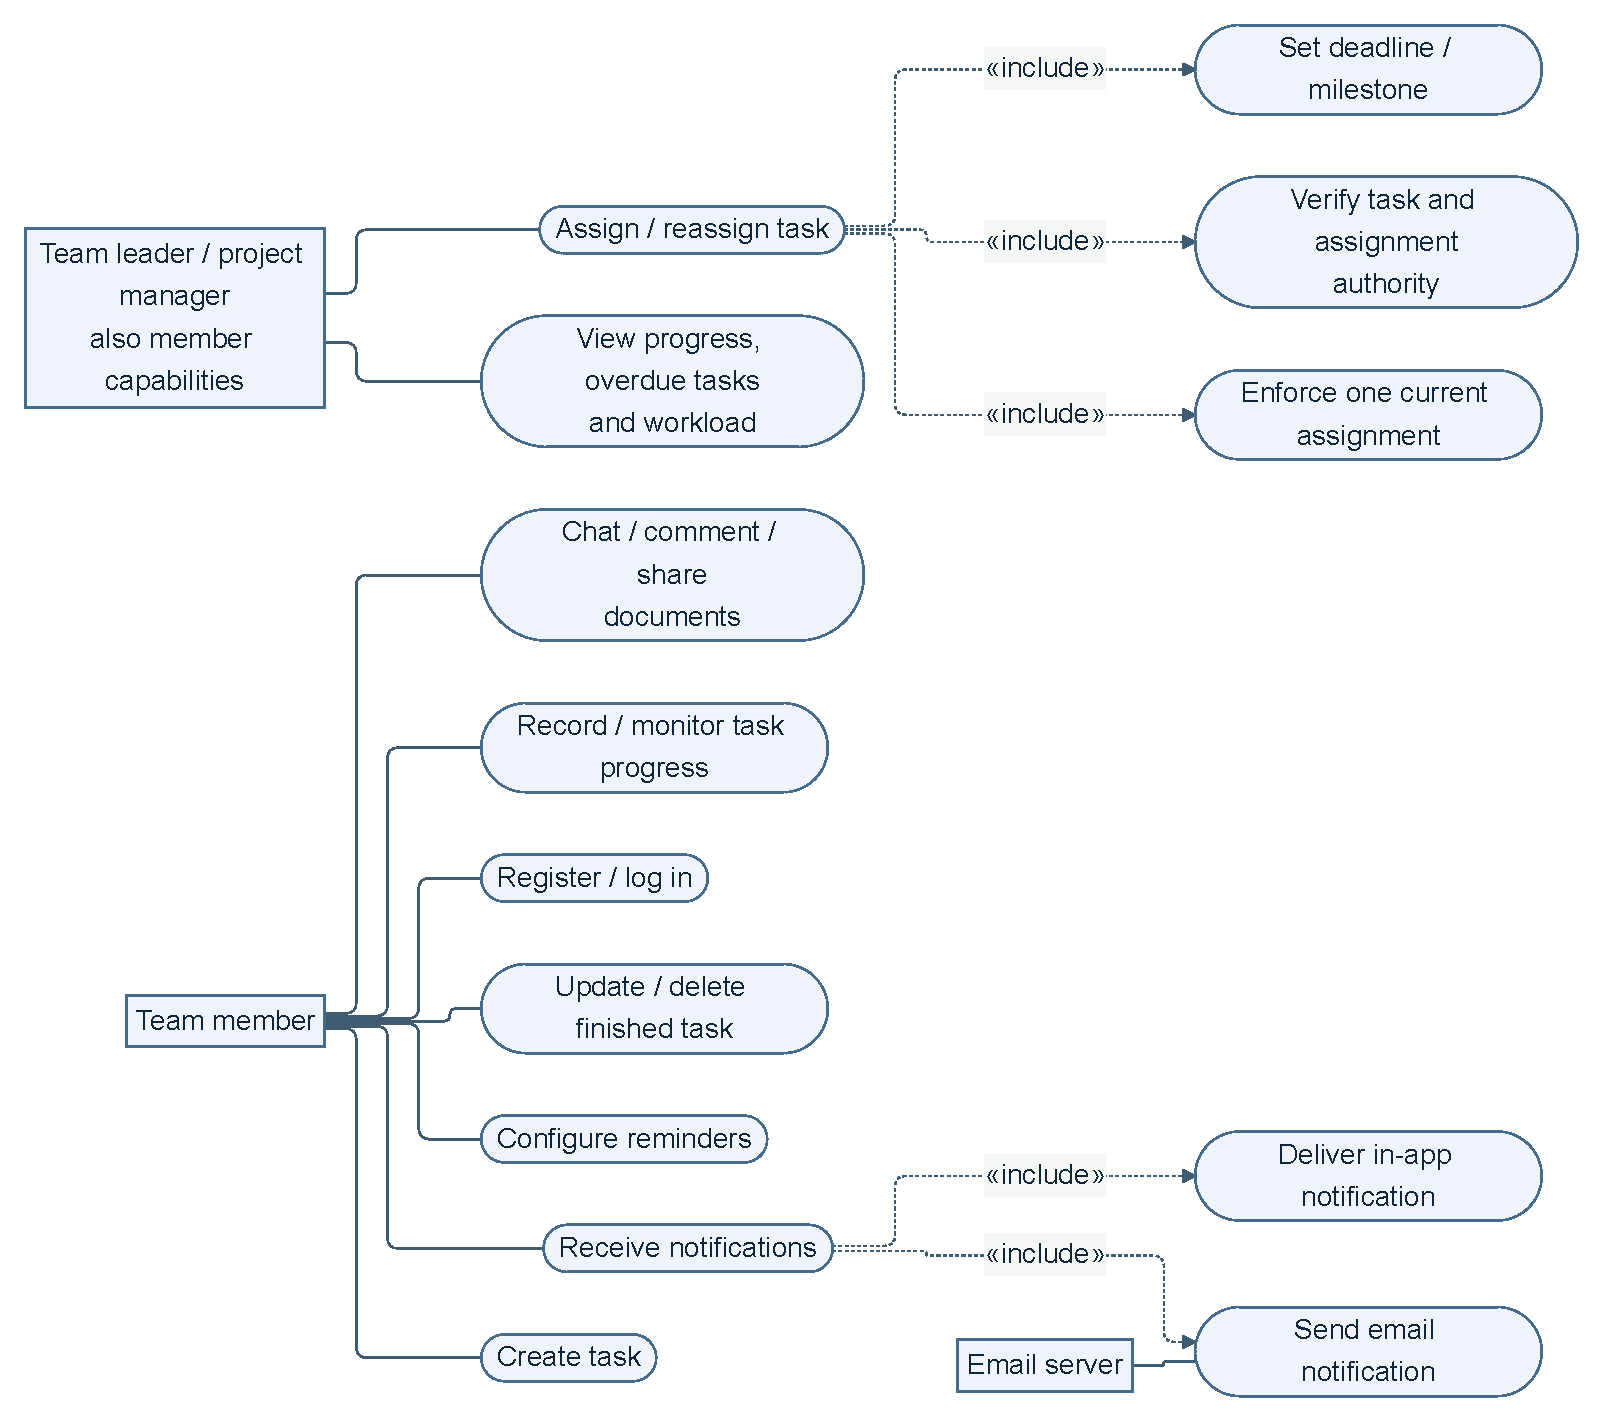
\includegraphics[width=451.44pt]{images/fig-069.pdf}
\captionof{figure}{Q1 --- Use cases (25 marks)}\end{minipage}\par\smallskip

\begin{studycolumns}
\vspace{0pt}



Every protected action requires a valid session and appropriate role. Member permissions for modifying/\allowbreak{}deleting tasks must follow the agreed access policy; the appendix does not say every member can modify every task. Include categorisation/\allowbreak{}priority/\allowbreak{}tag fields in Create/\allowbreak{}Update Task descriptions rather than treating each field entry as a separate user goal. No optional extension is needed simply to satisfy the diagram wording.

\textbf{(b) Use case: Assign Task.} Primary actor: authenticated Team Leader or Project Manager. Preconditions: task exists and actor is authorised; chosen individual/\allowbreak{}team exists. Normal flow: actor selects task; system presents task and current assignment; actor verifies task, chooses one assignee and specifies deadline/\allowbreak{}milestones; system validates rights and details; system atomically records the assignment and exposes updated workload/\allowbreak{}progress. Alternatives: unverified/\allowbreak{}invalid task or unavailable assignee, request correction; unauthorised actor, reject; concurrent assignment change, reject/\allowbreak{}reload; reassignment, replace the old assignment atomically instead of appending a second active assignment. \textbf{Assumption:} ``one assignment'' means one assignee target, which may be an individual or a team, not only one person within a team.

\needspace{4\baselineskip}
\subsection*{Q2 --- Analysis, lifecycle and process (25 marks)}
\sectionlabel{h-q2--analysis-lifecycle-and-process-25-marks}
\textbf{(a) Assignment conceptual classes/\allowbreak{}stereotypes (9). (b) Activity/\allowbreak{}swimlane diagram from task creation to deletion (7). (c) Waterfall response to drastic mid-project requirement change (4). (d) Improve customer satisfaction after a disappointing first agile sprint (5).}


\textbf{(a)}
\end{studycolumns}


\par\smallskip\noindent\begin{minipage}{\linewidth}\centering
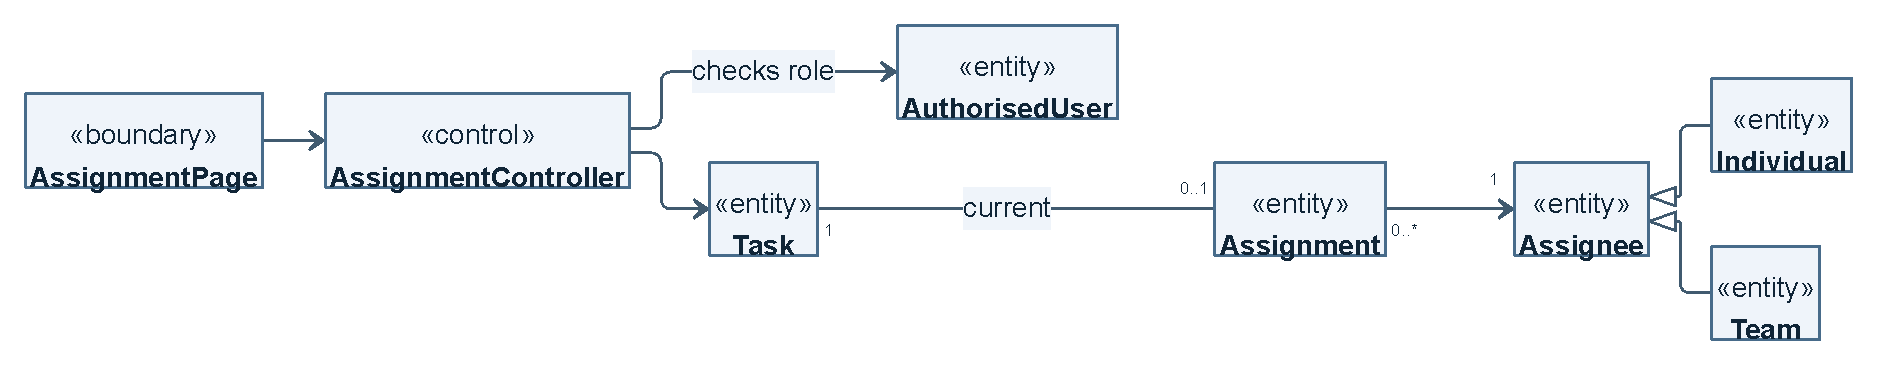
\includegraphics[width=514.00pt]{images/fig-070.pdf}
\captionof{figure}{Q2 --- Analysis, lifecycle and process (25 marks)}\end{minipage}\par\smallskip



If assignment history is added, use \code{0.\allowbreak{}.\allowbreak{}*} historical assignments plus an explicit \textbf{at most one active assignment} constraint; do not remove the invariant.

\textbf{(b)} The appendix permits update/\allowbreak{}deletion after completion, so those actions appear after Finished. Reassignment is an atomic replacement. Deletion is optional, not an automatic consequence of finishing.







\par\smallskip\noindent\begin{minipage}{\linewidth}\centering
{\scriptsize\textbf{A: create, verify and assign}}\par\smallskip
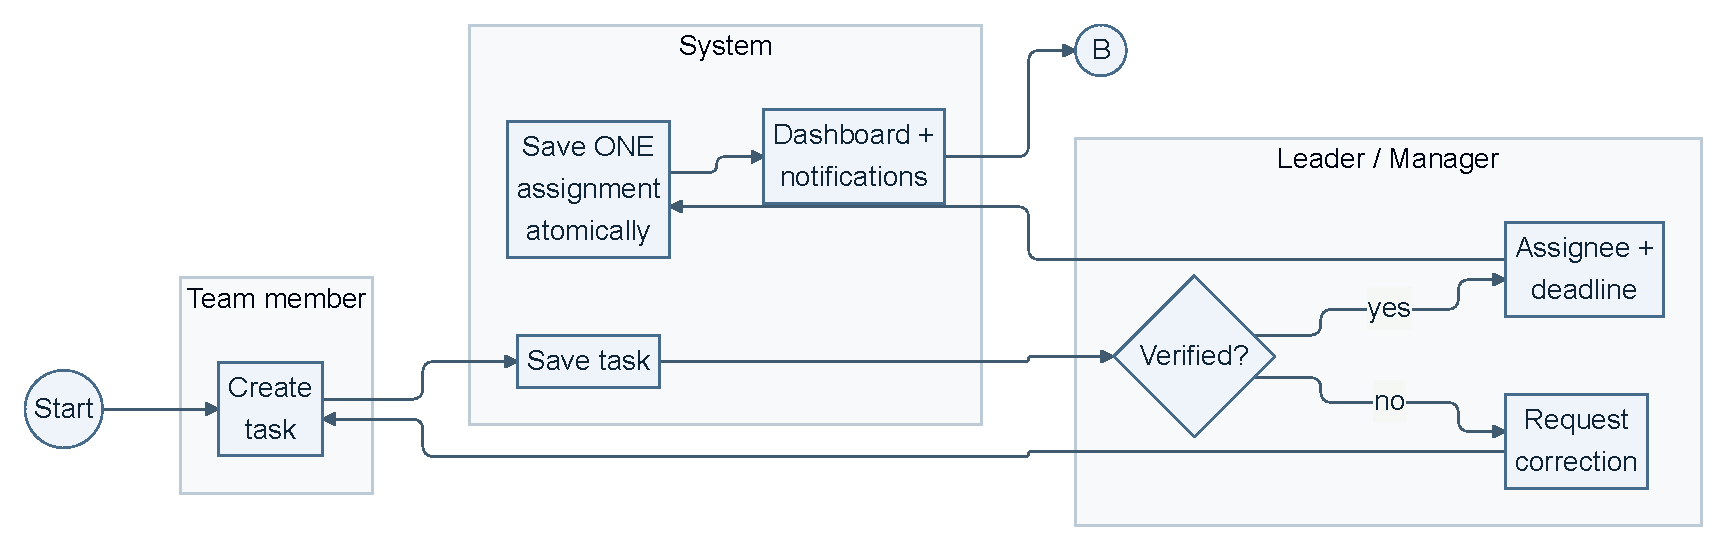
\includegraphics[width=442.00pt]{images/fig-071-a.pdf}\par\smallskip
{\scriptsize\textbf{B: work, reassign or finish}}\par\smallskip
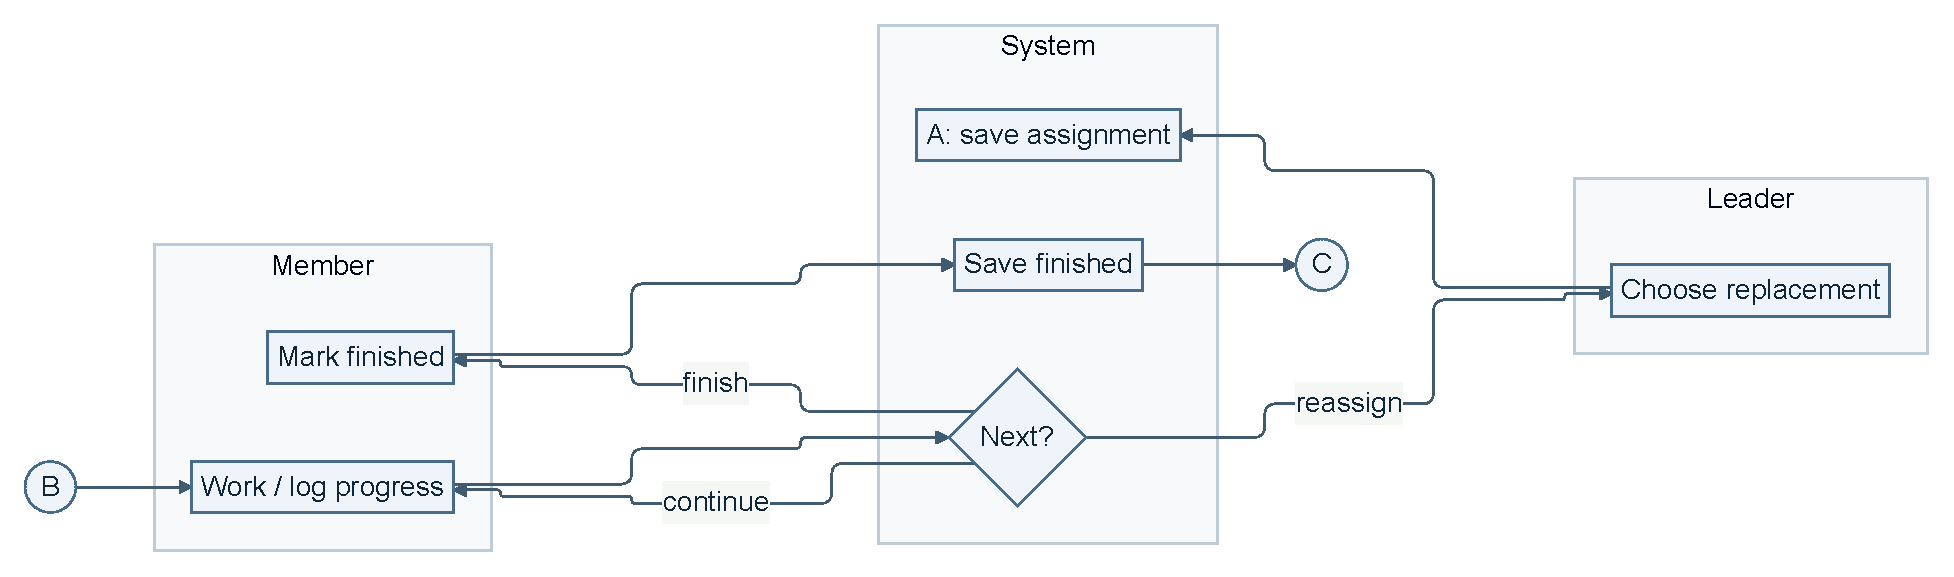
\includegraphics[width=500.00pt]{images/fig-071-b.pdf}\par\smallskip
{\scriptsize\textbf{C: authorised finished-task actions}}\par\smallskip
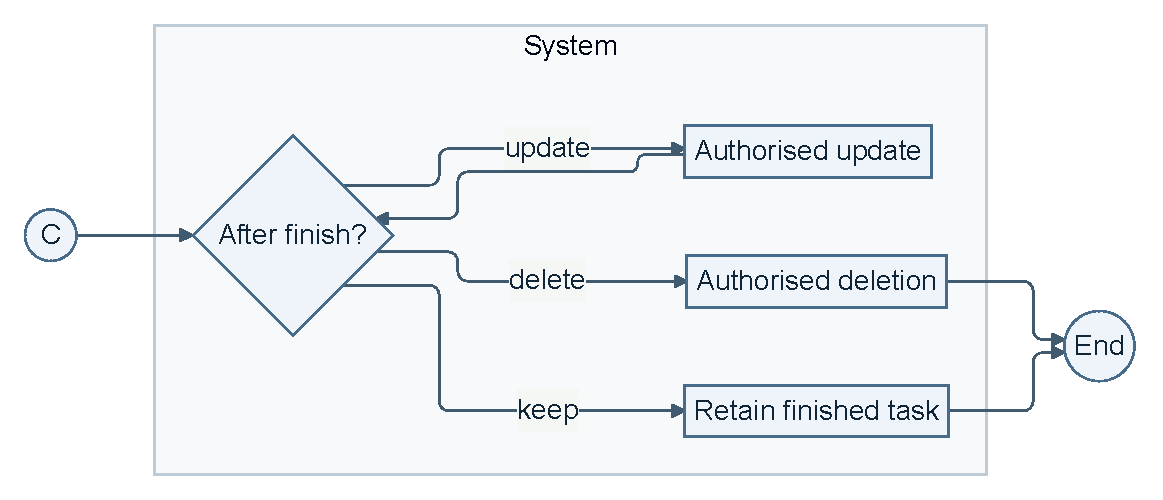
\includegraphics[width=297.20pt]{images/fig-071-c.pdf}\par\smallskip
\captionof{figure}{Q2 --- Analysis, lifecycle and process (25 marks) --- B/C continue below; A returns to atomic assignment.}\end{minipage}\par\smallskip

\begin{studycolumns}
\vspace{0pt}













\textbf{(c)} Apply \hyperref[answer-waterfall]{W, p.\ \pageref{answer-waterfall}} to the drastic task-system change; update affected artefacts and agree revised scope/schedule. Persistent change may justify incremental/agile delivery.

\textbf{(d)} Apply \hyperref[answer-scrum]{S, p.\ \pageref{answer-scrum}}: clarify unmet needs/acceptance criteria, reprioritise value with the PO, choose smaller usable increments and retrospect on estimates/capacity/integration.

\needspace{4\baselineskip}
\subsection*{Q3 --- Architecture, NFR and patterns (25 marks)}
\sectionlabel{h-q3--architecture-nfr-and-patterns-25-marks}
\textbf{(a)(i) Detailed architecture/\allowbreak{}classes (8); (ii) one relevant NFR and alternative architecture addressing it (8). (b)(i) Combined-pattern scenario/\allowbreak{}classes (6); (ii) is combining patterns always beneficial? (3).}


\textbf{(a)(i)} Use a layered task application: UI boundaries, application services, task/\allowbreak{}assignment entities and repositories/\allowbreak{}notification gateways.
\end{studycolumns}


\par\smallskip\noindent\begin{minipage}{\linewidth}\centering
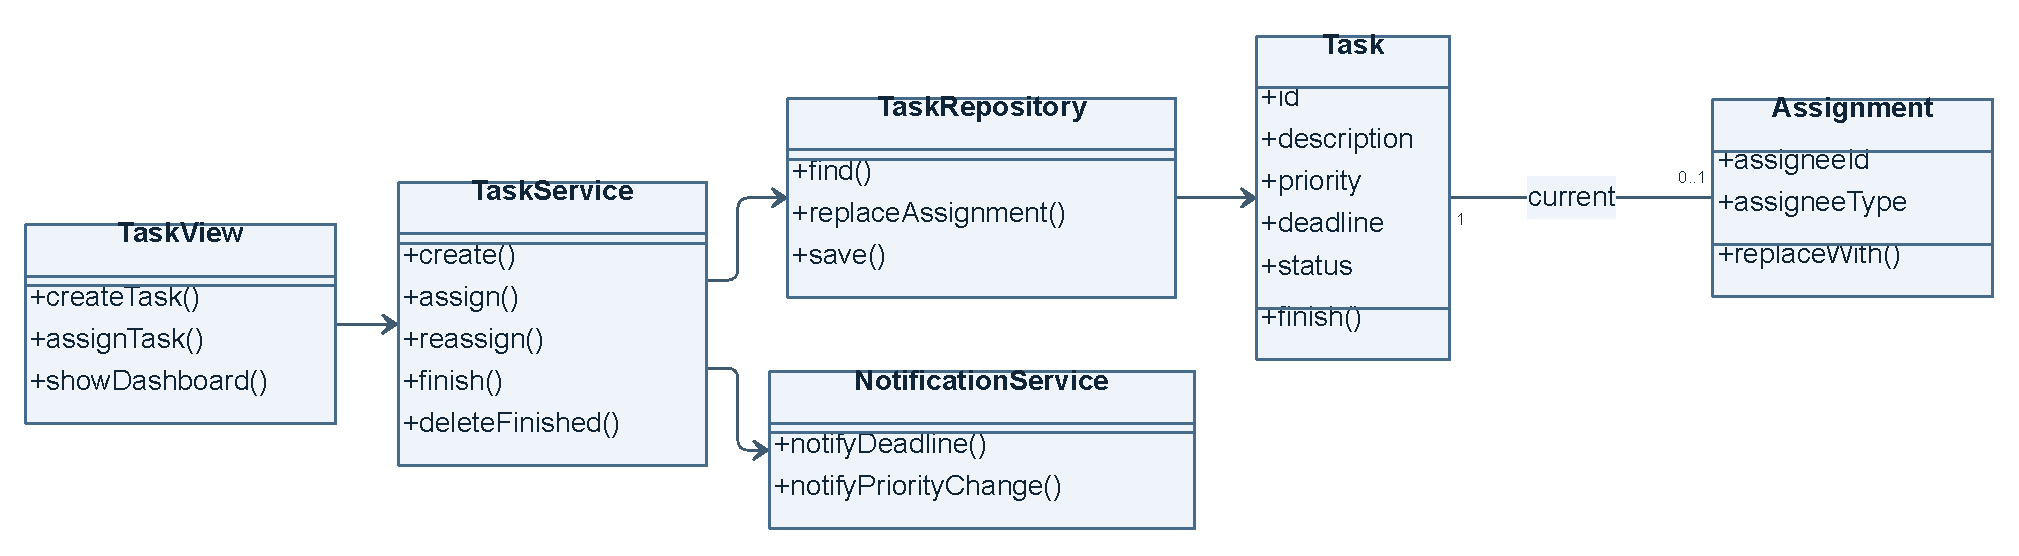
\includegraphics[width=514.00pt]{images/fig-072.pdf}
\captionof{figure}{Q3 --- Architecture, NFR and patterns (25 marks) --- assignment replacement is atomic}\end{minipage}\par\smallskip



\textbf{(a)(ii)} Choose \textbf{security/\allowbreak{}access control}, explicitly motivated by role-based access and sensitive team information. An alternative centralised \textbf{client--server architecture with a security Facade} places all task operations behind authenticated server-side authorisation. Browser/\allowbreak{}UI role checks alone cannot protect the data.




\par\smallskip\noindent\begin{minipage}{\linewidth}\centering
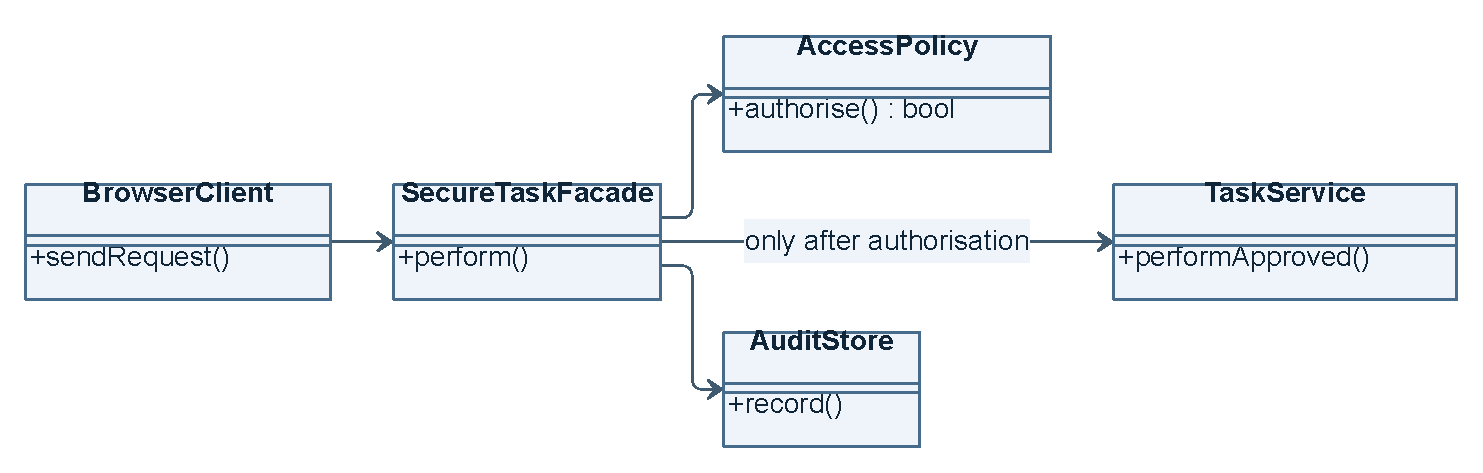
\includegraphics[width=417.56pt]{images/fig-073.pdf}
\captionof{figure}{Q3 --- Architecture, NFR and patterns (25 marks)}\end{minipage}\par\smallskip

\begin{studycolumns}
\vspace{0pt}



Keep Task/\allowbreak{}Assignment/\allowbreak{}Repository from Q3(a)(i) behind TaskService. Centralisation makes policy consistent across clients and supports audited denials; it adds a server/\allowbreak{}network dependency. Audit storage is a proposed security measure, not an explicit appendix feature. Layering and client--server are compatible architectural dimensions; the alternative adds a trust boundary rather than claiming that these styles are mutually exclusive.

\textbf{(b)(i)} Combine Observer with Simple Factory for email and in-app notifications. A task subject notifies both subscribed channels on relevant events; a factory creates/\allowbreak{}configures channel observers. Deadline timers also publish events rather than requiring a task to mutate every second.
\end{studycolumns}


\par\smallskip\noindent\begin{minipage}{\linewidth}\centering
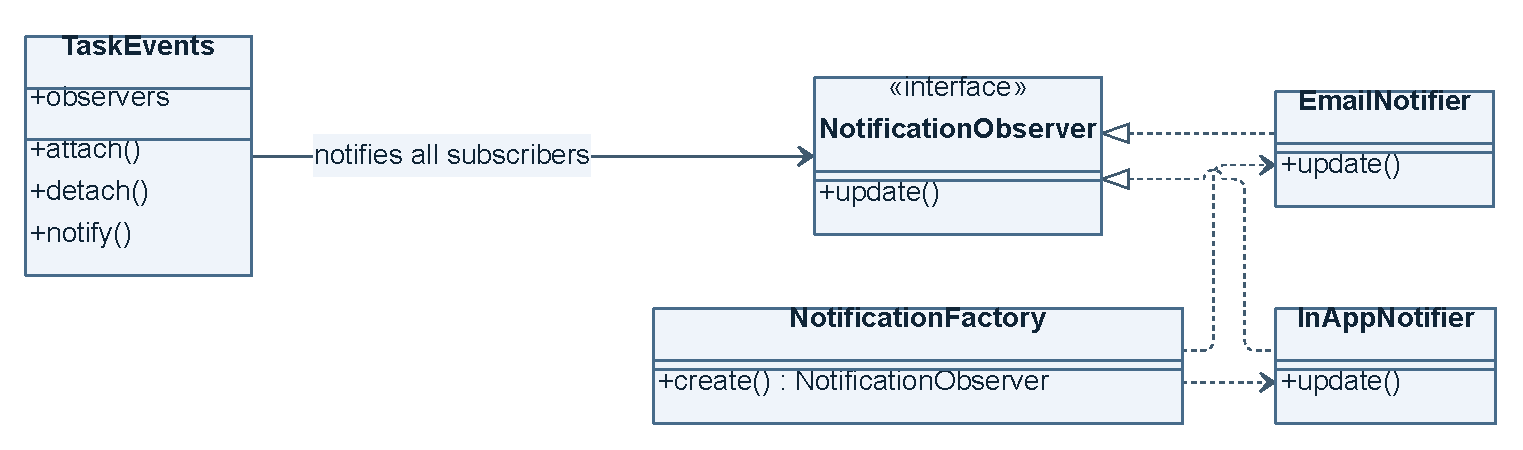
\includegraphics[width=428.56pt]{images/fig-074.pdf}
\captionof{figure}{Q3 --- Architecture, NFR and patterns (25 marks)}\end{minipage}\par\smallskip

\begin{studycolumns}
\vspace{0pt}



Factory governs creation; Observer governs runtime notification without coupling task code to concrete delivery channels. The requirements call for email \textbf{and} in-app messages, not arbitrarily selecting only one.

\textbf{(b)(ii)} No: apply \hyperref[answer-pattern-cost]{C, p.\ \pageref{answer-pattern-cost}}. Email and in-app notifications justify separate channels; unrelated patterns add cost without solving another force.

\needspace{4\baselineskip}
\subsection*{Q4 --- Task inputs, shift-left and maintenance (25 marks)}
\sectionlabel{h-q4--task-inputs-shift-left-and-maintenance-25-marks}
\textbf{(a)(i) Derive ECs for Task Description, Resource needed, Deadline and Task Priority (4). (ii) Give on/\allowbreak{}below/\allowbreak{}above boundary values (4). (iii) Design defensive tests (5).}


\textbf{Input interpretation.} Task Description must be ASCII; Resource needed is a 4-digit integer; Deadline is between 2024 and 2026; Task Priority is one of \code{Critical}, \code{High}, \code{Normal}, \code{Low}, \code{Very Low}. Assume a positive 4-digit numeric value (not a string whose leading zeroes count as digits), inclusive complete calendar years, and one-day date resolution. These interpretations are stated because the brief does not specify parsing details. Do not invent an ASCII-field length limit.

\textbf{(i) Equivalence classes:}
\end{studycolumns}


{\fontsize{8.5}{9.8}\selectfont
\begin{longtable}{L{\dimexpr 0.22368\linewidth-5.37pt\relax}L{\dimexpr 0.33177\linewidth-7.96pt\relax}L{\dimexpr 0.44455\linewidth-10.67pt\relax}}
\toprule
\rowcolor{ice}\textbf{Field} & \textbf{Valid EC} & \textbf{Invalid ECs} \\
\midrule\endfirsthead
\toprule\rowcolor{ice}\textbf{Field} & \textbf{Valid EC} & \textbf{Invalid ECs} \\
\midrule\endhead
\multicolumn{3}{r}{\scriptsize Continued on next page}\\\endfoot
\bottomrule\endlastfoot
Task Description & ASCII text & Text containing non-ASCII characters \\
Resource needed & Integer 1000\ldots{}9999 & Integer below 1000; integer above 9999; malformed/\allowbreak{}non-integer input at the input boundary \\
Deadline & Real calendar date 2024-01-01\ldots{}2026-12-31 & Real date before 2024-01-01; real date after 2026-12-31; malformed/\allowbreak{}nonexistent date \\
Task Priority & One EC containing \{Critical, High, Normal, Low, Very Low\} & Any unlisted value \\
\end{longtable}
}

The category set is \textbf{one valid EC}, although testing all its few members is useful. No empty-string prohibition or printable-only ASCII restriction is supplied; clarify those separately instead of asserting an invented oracle.

\textbf{(ii) Boundary triplets:}




{\fontsize{8.5}{9.8}\selectfont
\begin{longtable}{L{\dimexpr 0.27680\linewidth-8.86pt\relax}L{\dimexpr 0.23890\linewidth-7.64pt\relax}L{\dimexpr 0.24215\linewidth-7.75pt\relax}L{\dimexpr 0.24215\linewidth-7.75pt\relax}}
\toprule
\rowcolor{ice}\textbf{Field /\allowbreak{} boundary} & \textbf{Just below} & \textbf{On boundary} & \textbf{Just above} \\
\midrule\endfirsthead
\toprule\rowcolor{ice}\textbf{Field /\allowbreak{} boundary} & \textbf{Just below} & \textbf{On boundary} & \textbf{Just above} \\
\midrule\endhead
\multicolumn{4}{r}{\scriptsize Continued on next page}\\\endfoot
\bottomrule\endlastfoot
Resource needed: minimum & 999 (reject) & 1000 (accept) & 1001 (accept) \\
Resource needed: maximum & 9998 (accept) & 9999 (accept) & 10000 (reject) \\
Deadline: earliest & 2023-12-31 (reject) & 2024-01-01 (accept) & 2024-01-02 (accept) \\
Deadline: latest & 2026-12-30 (accept) & 2026-12-31 (accept) & 2027-01-01 (reject) \\
\end{longtable}
}

ASCII membership and unordered categories have no specified application-level ordered boundary. Malformed values are additional EC tests, not numeric/\allowbreak{}date neighbours.

\textbf{(iii) Defensive suite.} Use the common testing conventions below; valid rows combine boundaries, invalid rows isolate one field. The full boundary suite is retained.




{\fontsize{8.5}{9.8}\selectfont
\begin{longtable}{L{\dimexpr 0.18631\linewidth-7.45pt\relax}L{\dimexpr 0.16907\linewidth-6.76pt\relax}L{\dimexpr 0.16907\linewidth-6.76pt\relax}L{\dimexpr 0.16907\linewidth-6.76pt\relax}L{\dimexpr 0.30647\linewidth-12.26pt\relax}}
\toprule
\rowcolor{ice}\textbf{Task Description} & \textbf{Resource needed} & \textbf{Deadline} & \textbf{Task Priority} & \textbf{Expected /\allowbreak{} purpose} \\
\midrule\endfirsthead
\toprule\rowcolor{ice}\textbf{Task Description} & \textbf{Resource needed} & \textbf{Deadline} & \textbf{Task Priority} & \textbf{Expected /\allowbreak{} purpose} \\
\midrule\endhead
\multicolumn{5}{r}{\scriptsize Continued on next page}\\\endfoot
\bottomrule\endlastfoot
\code{Implement API} & \code{1000} & \code{2024-\allowbreak{}01-\allowbreak{}01} & \code{Critical} & Accept --- valid boundaries /\allowbreak{} category coverage \\
\code{Implement API} & \code{1001} & \code{2024-\allowbreak{}01-\allowbreak{}02} & \code{High} & Accept --- valid boundaries /\allowbreak{} category coverage \\
\code{Implement API} & \code{9998} & \code{2026-\allowbreak{}12-\allowbreak{}30} & \code{Normal} & Accept --- valid boundaries /\allowbreak{} category coverage \\
\code{Implement API} & \code{9999} & \code{2026-\allowbreak{}12-\allowbreak{}31} & \code{Low} & Accept --- valid boundaries /\allowbreak{} category coverage \\
\code{Implement API} & \code{5499} & \code{2025-\allowbreak{}07-\allowbreak{}01} & \code{Very Low} & Accept --- interior baseline /\allowbreak{} category coverage \\
\code{caf\'{e}} & \code{5499} & \code{2025-\allowbreak{}07-\allowbreak{}01} & \code{Critical} & Reject --- non-ASCII Task Description \\
\code{Implement API} & \code{999} & \code{2025-\allowbreak{}07-\allowbreak{}01} & \code{Critical} & Reject --- Resource needed below minimum \\
\code{Implement API} & \code{10000} & \code{2025-\allowbreak{}07-\allowbreak{}01} & \code{Critical} & Reject --- Resource needed above maximum \\
\code{Implement API} & \code{5499} & \code{2023-\allowbreak{}12-\allowbreak{}31} & \code{Critical} & Reject --- Deadline below minimum \\
\code{Implement API} & \code{5499} & \code{2027-\allowbreak{}01-\allowbreak{}01} & \code{Critical} & Reject --- Deadline above maximum \\
\code{Implement API} & \code{5499} & \code{2025-\allowbreak{}07-\allowbreak{}01} & \code{Unknown} & Reject --- unlisted Task Priority \\
\code{Implement API} & \code{12x} & \code{2025-\allowbreak{}07-\allowbreak{}01} & \code{Critical} & Reject --- malformed integer; extra defensive case \\
\code{Implement API} & \code{5499} & \code{2024-\allowbreak{}02-\allowbreak{}30} & \code{Critical} & Reject --- nonexistent calendar date; extra defensive case \\
\end{longtable}
}

\begin{studycolumns}
\vspace{0pt}

\textbf{(b) Why is shift-left testing useful? (4). (c) Four maintenance challenges and mitigations (8).}


\textbf{(b)} Reviewing requirements and designing tests early exposes ambiguity before it spreads into design/\allowbreak{}code. Early unit/\allowbreak{}integration automation provides fast feedback, reduces downstream rework and makes changes safer. Examples: identify the one-assignment invariant during analysis and test the service before building the dashboard. Shift-left complements rather than eliminates later system, performance and acceptance testing.

\textbf{(c)}
\end{studycolumns}


{\fontsize{8.5}{9.8}\selectfont
\begin{longtable}{L{\dimexpr 0.38681\linewidth-6.19pt\relax}L{\dimexpr 0.61319\linewidth-9.81pt\relax}}
\toprule
\rowcolor{ice}\textbf{Challenge} & \textbf{Mitigation} \\
\midrule\endfirsthead
\toprule\rowcolor{ice}\textbf{Challenge} & \textbf{Mitigation} \\
\midrule\endhead
\multicolumn{2}{r}{\scriptsize Continued on next page}\\\endfoot
\bottomrule\endlastfoot
Understanding unfamiliar/\allowbreak{}poorly documented legacy code & Maintain architecture/\allowbreak{}decision notes, clear interfaces and traceable change history; use code reviews and onboarding. \\
Regressions caused by changes & Automate regression tests, check integration/\allowbreak{}compatibility, and use reviewed version-controlled changes with rollback. \\
Increasing technical debt and coupling & Refactor incrementally with behaviour-preservation checks; keep responsibilities and boundaries clear. \\
Changing requirements/\allowbreak{}dependencies and operational environments & Perform impact analysis, prioritise changes, maintain supported dependency versions, and update requirements/\allowbreak{}tests/\allowbreak{}documentation together. \\
\end{longtable}
}

Tie each challenge to its remedy rather than listing four generic ``best practices'' without explanation.


\par\Needspace{120pt}\medskip
\section*{Paper 6: AY2024/\allowbreak{}25 Semester 2 --- Disaster Warning System (DWS)}\label{paper-2425-s2}
\phantomsection\addcontentsline{toc}{section}{Paper 6: AY2024/25 Semester 2 --- Disaster Warning System (DWS)}\markboth{AY2024/25 S2}{}
\sectionlabel{h-182-ay202425-semester-2--disaster-warning-system-dws}
\textbf{Source:} \href{run:/Users/bryangoh/Work/ntu-cs/sc2006/pyps/SC2006\_AY2425\_S2\_Questions.pdf}{Question paper}, Q1--Q4 on PDF pp. 1--4; Appendix A on p. 5.




\begin{studycolumns}
\vspace{0pt}
\textbf{Case facts.} A local government deploys a configurable DWS. Its manager registers/\allowbreak{}deregisters physically connected sensors and alert systems, links/\allowbreak{}unlinks registered sensor--alert pairs, and chooses safe measurement ranges. Registered sensors send integer updates at any time; an out-of-range value triggers the linked alert. Changes and received/\allowbreak{}sent messages are recorded. More than 24 hours without an update from a registered sensor causes a manager alert. The manager can retrieve the full record.

\needspace{4\baselineskip}
\subsection*{Q1 --- Stakeholders, requirements and use cases (25 marks)}
\sectionlabel{h-q1--stakeholders-requirements-and-use-cases-25-marks}
\textbf{(a) Four stakeholders and interests (4). (b) Three FRs and three NFRs (6). (c) Actors/\allowbreak{}use cases/\allowbreak{}relationships (15).}


\textbf{(a)} Local government: public safety, budget and dependable operation. DWS manager: correct configuration, sensor health and usable records. Emergency responders/\allowbreak{}alert recipients: timely, accurate, actionable warnings. Residents: protection from disasters and avoidance of missed/\allowbreak{}false alarms. A stakeholder need not directly operate the software and therefore need not be an actor.

\textbf{(b) Three FRs:} (1) accept sensor/\allowbreak{}alert registration only when physical connection is detected; (2) maintain configured links/\allowbreak{}ranges and trigger linked alerts for out-of-range integer measurements; (3) notify the manager when a registered sensor has supplied no update for over 24 hours. Recording and record retrieval are additional FRs.

\textbf{Three proposed NFRs:} (1) flexibility/\allowbreak{}interoperability across different deployments and sensor/\allowbreak{}alert implementations; (2) availability/\allowbreak{}reliability for ongoing monitoring and fault recovery; (3) performance for timely processing and delivery of alerts under the agreed peak sensor workload. Flexibility is explicit in the case; measurable availability, latency and recovery targets must be agreed, not invented. ``Log all messages'' is functional behaviour, not automatically an NFR merely because it concerns auditing.

\textbf{(c)} Actors: DWS Manager, external Sensor, external Alert System. Time passage is an event, not necessarily an actor.
\end{studycolumns}


\par\smallskip\noindent\begin{minipage}{\linewidth}\centering
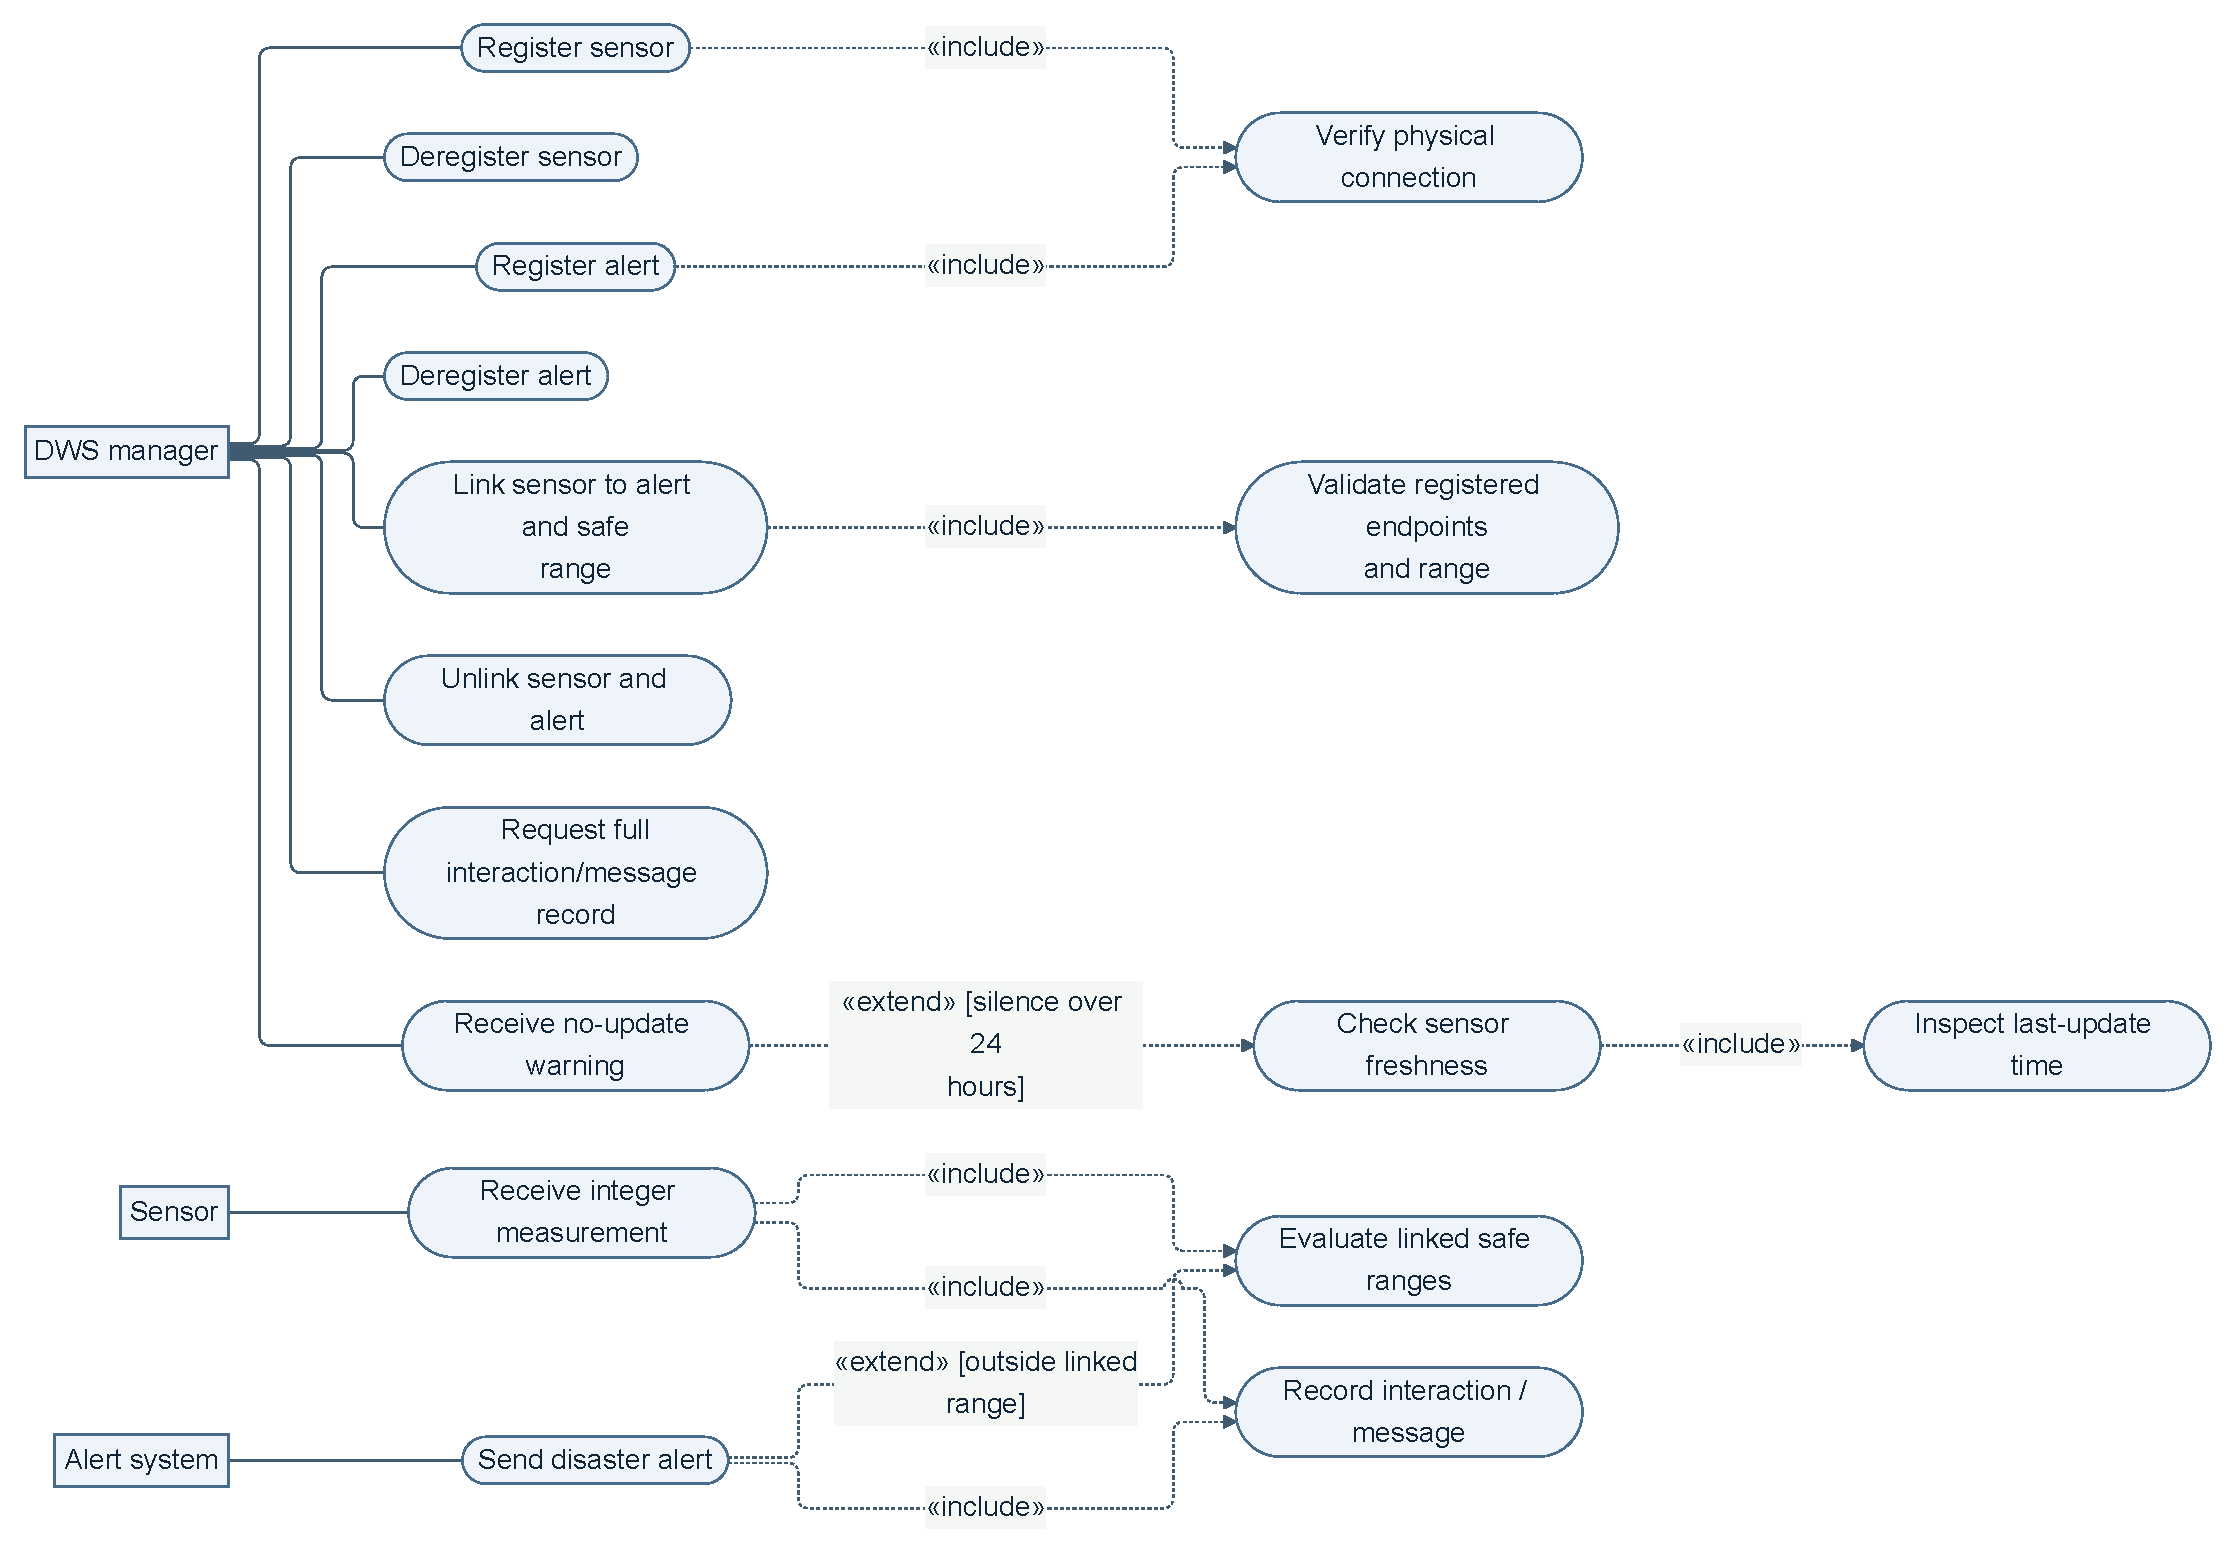
\includegraphics[width=514.00pt]{images/fig-075.pdf}
\captionof{figure}{Q1 --- Stakeholders, requirements and use cases (25 marks)}\end{minipage}\par\smallskip

\begin{studycolumns}
\vspace{0pt}













Registration, deregistration, linking and unlinking also include recording; add their arrows to the shared Record use case in exact UML. The physical-connection check applies only to registration. Safe-range alerting is conditional, making \code{\guillemotleft{}extend\guillemotright{}} reasonable here. The system must not let an unregistered sensor bypass its configured registration policy.

\needspace{4\baselineskip}
\subsection*{Q2 --- Sensor behaviour and process (25 marks)}
\sectionlabel{h-q2--sensor-behaviour-and-process-25-marks}
\textbf{(a) Sensor-object state machine (6). (b) Linking activity/\allowbreak{}swimlanes (7). (c)(i) Choose Waterfall or Agile for changing requirements (3); (ii) manage changes (3). (d) Scrum response to an urgent mid-sprint feature request (6).}


\textbf{(a)} Model the sensor's \textbf{DWS-side lifecycle}, since this software cannot dictate the internal hardware's physical operating states. A registered sensor is monitored even when quiet; silence is not automatic deregistration. A registration timestamp starts monitoring until the first update, a necessary stated assumption because the appendix does not define that initial timer.
\end{studycolumns}


\par\smallskip\noindent\begin{minipage}{\linewidth}\centering
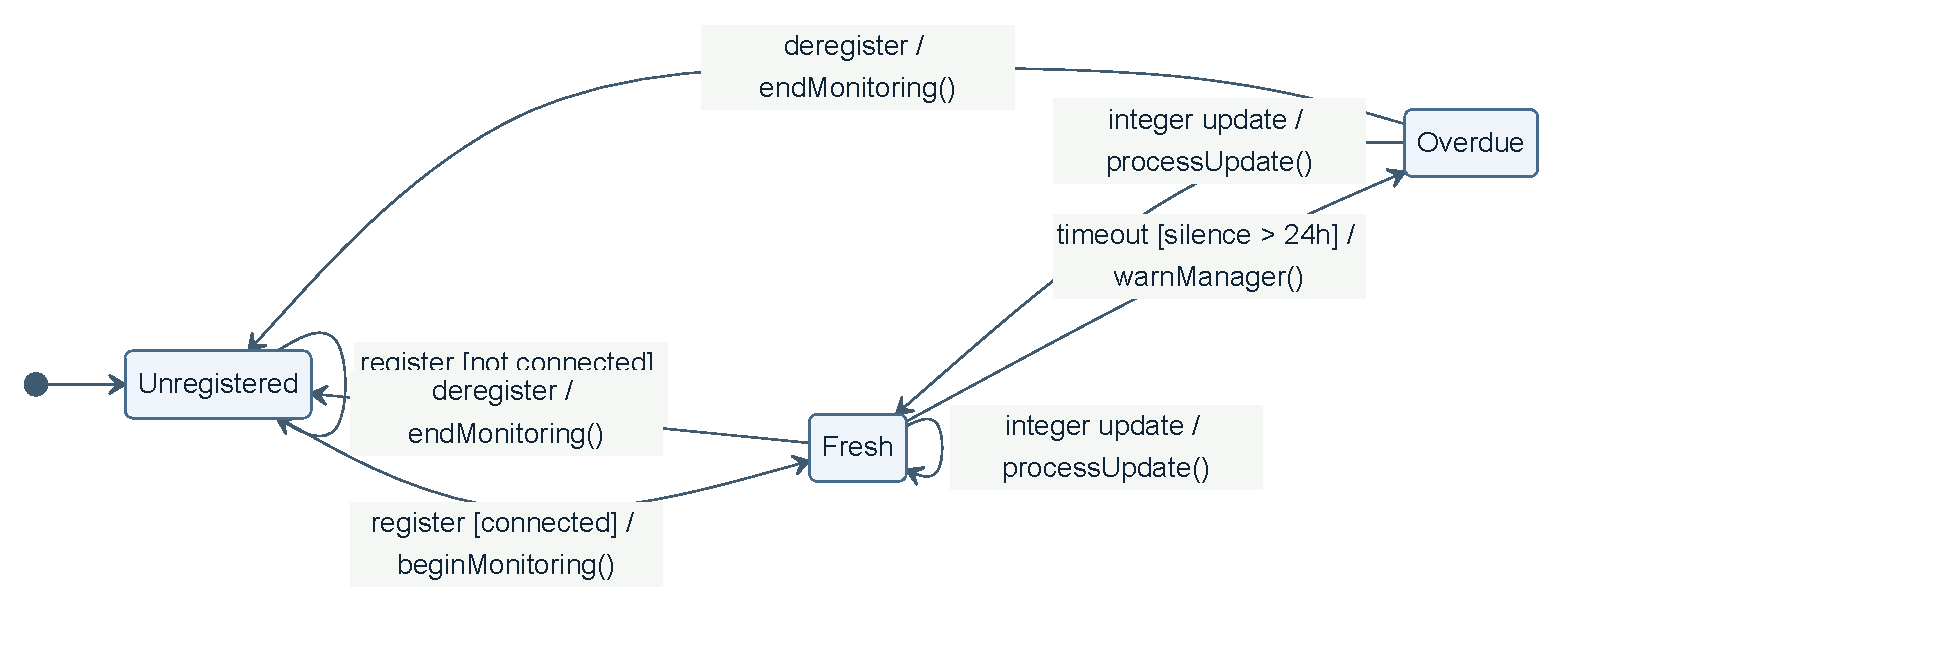
\includegraphics[width=514.00pt]{images/fig-076.pdf}
\captionof{figure}{Q2 --- Sensor behaviour and process (25 marks)}\end{minipage}\par\smallskip





\code{begin\allowbreak{}Monitoring()} records registration and starts freshness timing; \code{process\allowbreak{}Update()} records the valid measurement, evaluates linked ranges and resets freshness; \code{end\allowbreak{}Monitoring()} records deregistration and stops monitoring/\allowbreak{}subscriptions. Exactly 24 hours is not ``over 24 hours''. Repeated warning frequency is unspecified; assume one warning per overdue episode unless the client defines reminders. Invalid-type messages are rejected/\allowbreak{}logged by a defensive integration boundary, not treated as valid measurements.

\textbf{(b)}






\par\smallskip\noindent\begin{minipage}{\linewidth}\centering
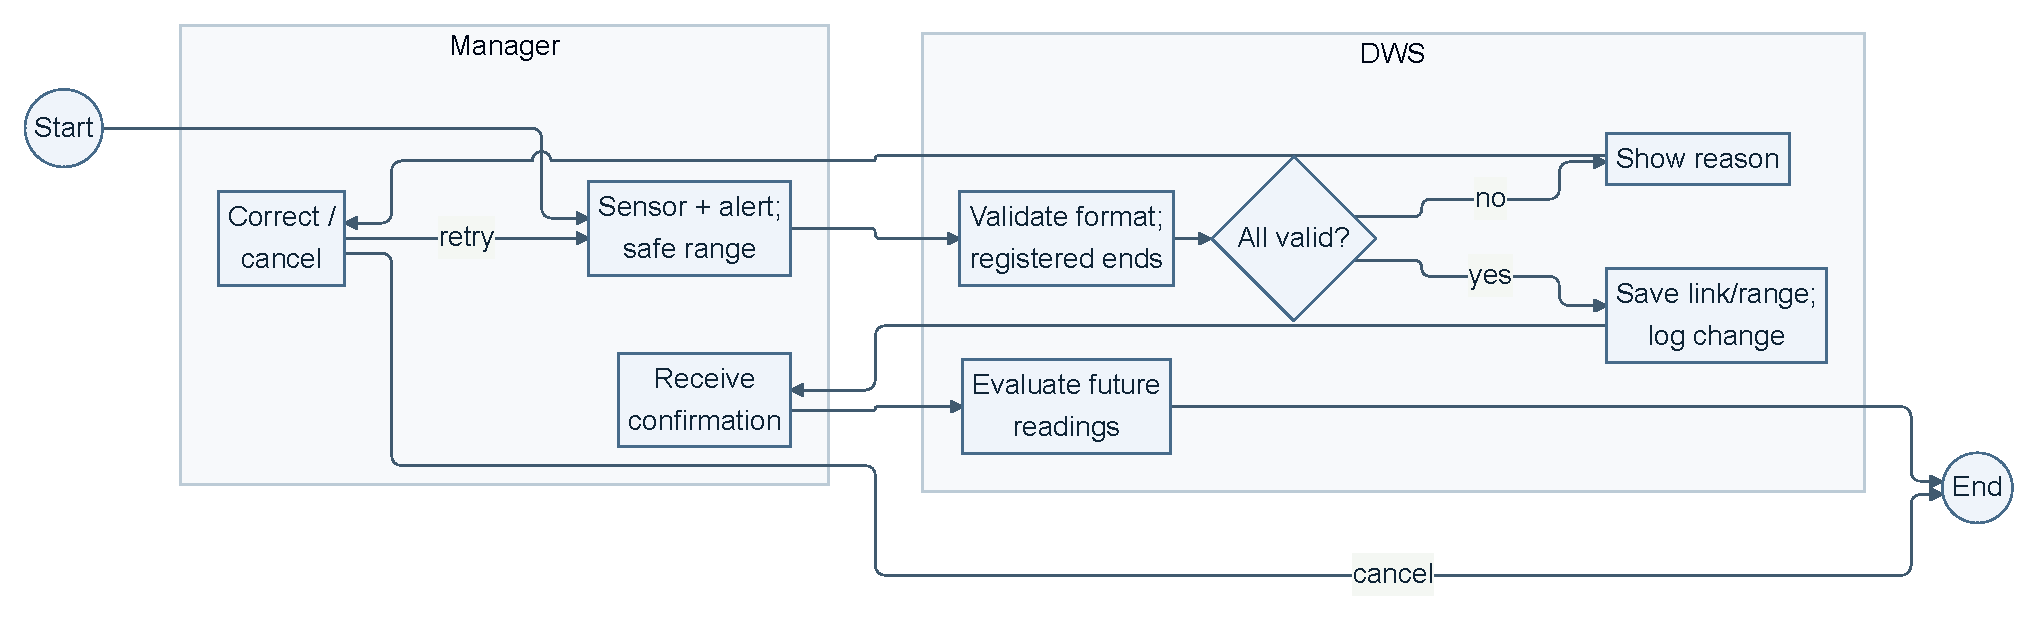
\includegraphics[width=514.00pt]{images/fig-077.pdf}
\captionof{figure}{Q2 --- Sensor behaviour and process (25 marks)}\end{minipage}\par\smallskip

\begin{studycolumns}
\vspace{0pt}









Linking does not require an immediate disaster measurement, nor does it automatically send an alert. Preserve the existing configuration if validation fails.

\textbf{(c)(i)} Recommend Agile/\allowbreak{}incremental delivery because requirements may change and early stakeholder feedback can refine configuration and warning workflows. Retain appropriate safety reviews, documentation and rigorous testing; ``agile'' does not mean no planning.

\textbf{(c)(ii)} Capture changes in a prioritised backlog, clarify acceptance criteria, analyse safety/\allowbreak{}interface impacts and select feasible increments. Protect the current sprint's goal; negotiate later scope and re-estimate affected work, then validate changes with regression and acceptance tests.

\textbf{(d)} Use \hyperref[answer-scrum]{S, p.\ \pageref{answer-scrum}}: PO/developers assess urgency and goal impact; normally backlog the feature for a later sprint. Negotiate transparent scope changes; only the PO cancels an obsolete goal.

\needspace{4\baselineskip}
\subsection*{Q3 --- DWS architecture, Observer and responsibility (25 marks)}
\sectionlabel{h-q3--dws-architecture-observer-and-responsibility-25-marks}
\textbf{(a) Architecture/\allowbreak{}justification (3). (b)(i) Most applicable pattern (3); (ii) detailed classes (10). (c)(i) One reason for/\allowbreak{}against blaming the vendor for a crash on a string measurement (2); (ii) two other responsible parties (4); (iii) three prevention/\allowbreak{}risk-reduction measures (3).}


\textbf{(a)} An event-driven architecture, with layered configuration, monitoring/\allowbreak{}domain and device-integration services, fits asynchronous measurements. A registry manages runtime membership, a monitor evaluates configured links, and gateways deliver alerts while a record store preserves interactions. Isolate malformed or failing devices so one sensor cannot crash monitoring for all others.

\textbf{(b)(i)} \textbf{Observer}: sensor subjects publish measurements to a DWS observer that can subscribe/\allowbreak{}unsubscribe at runtime. This avoids tight coupling to a fixed sensor set and avoids requiring the DWS to synchronously poll for every update. Distinguish domain registration from subscription: the registration service coordinates both, but a list of objects alone is not Observer.

\textbf{(b)(ii)}
\end{studycolumns}


\par\smallskip\noindent\begin{minipage}{\linewidth}\centering
{\scriptsize\textbf{Observer protocol}}\par\smallskip
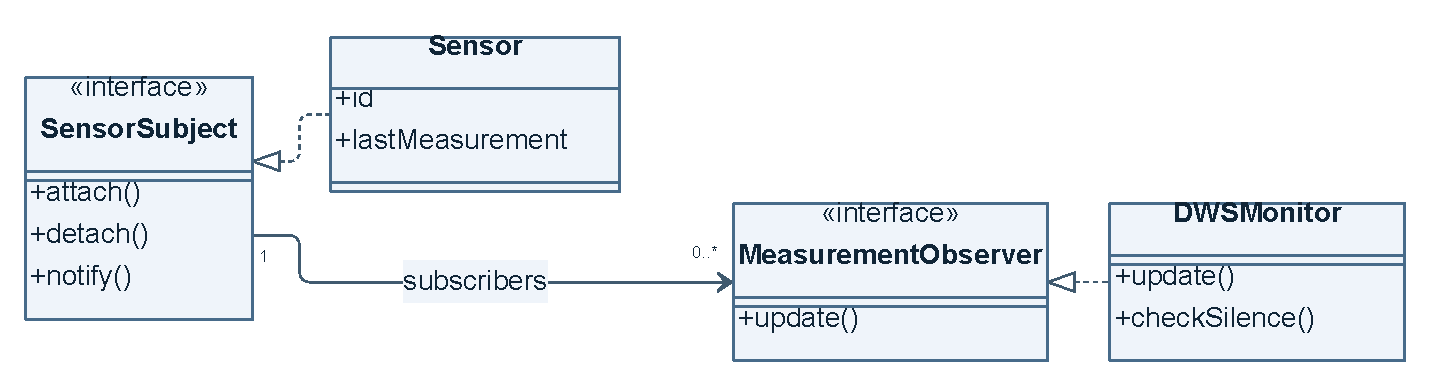
\includegraphics[width=366.00pt]{images/fig-078-protocol.pdf}\par\smallskip
{\scriptsize\textbf{DWS collaborations; DWSMonitor is shared}}\par\smallskip
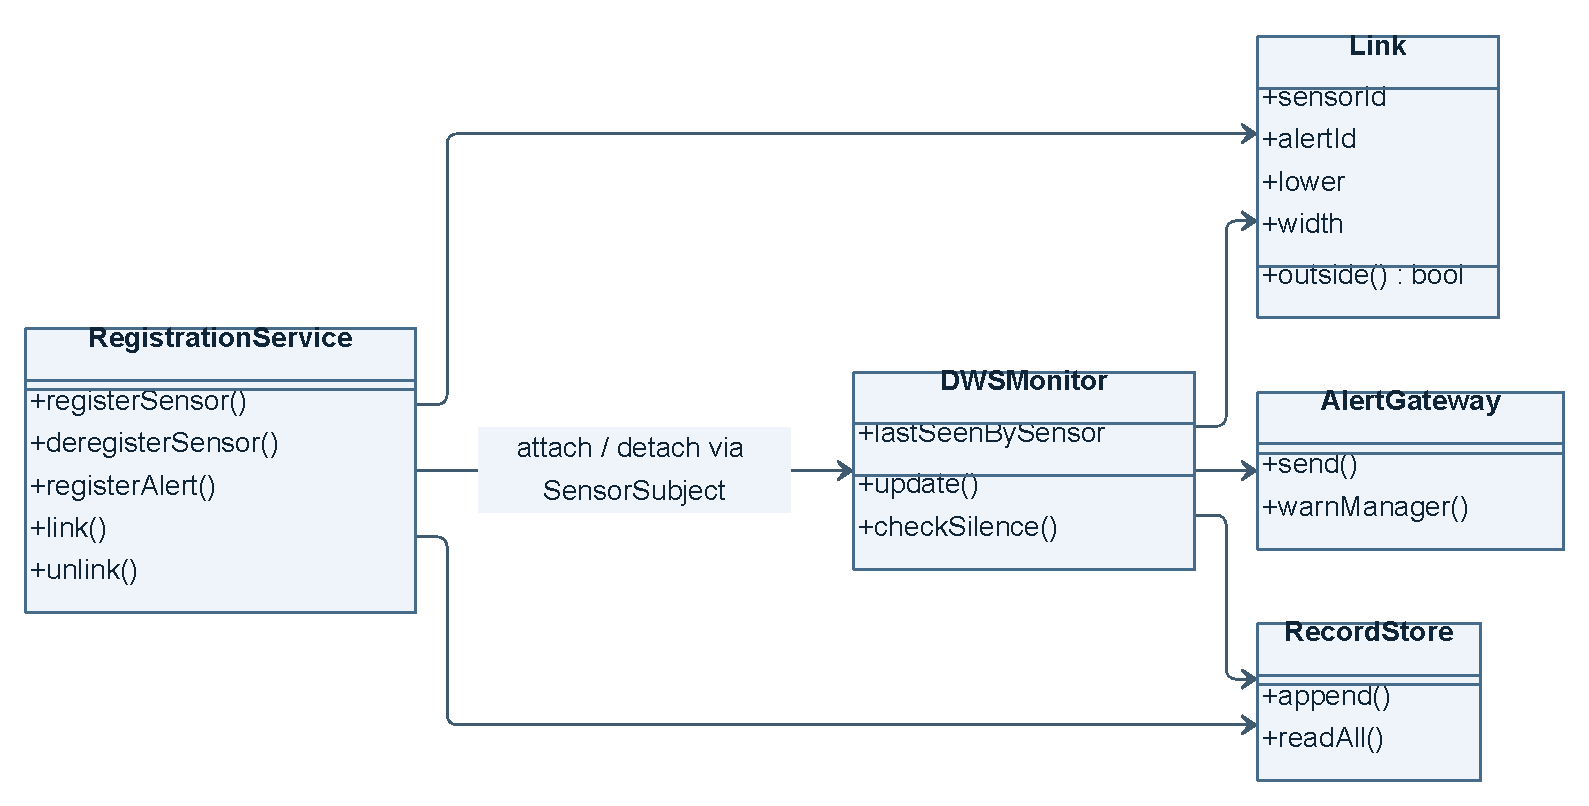
\includegraphics[width=406.80pt]{images/fig-078-services.pdf}\par\smallskip
\captionof{figure}{Q3 --- DWS architecture, Observer and responsibility (25 marks)}\end{minipage}\par\smallskip

\begin{studycolumns}
\vspace{0pt}









For heterogeneous external devices, a sensor adapter can expose SensorSubject while translating the real protocol. \code{update} validates integer messages, records them, updates freshness, evaluates every matching Link, and records any sent alerts. Registration verifies connection before subscribing. Link changes are recorded. Deregistration stops monitoring/\allowbreak{}subscriptions; the policy for dependent links must be agreed rather than leaving dangling references. Use overflow-safe arithmetic for safe-range calculations.

\textbf{(c)(i)} Engineering arguments \textbf{for} responsibility: a foreseeable malformed external input should be rejected/\allowbreak{}isolated rather than causing a system-wide outage, especially in a warning system. \textbf{Against:} the third-party sensor violated the specified integer interface contract; the DWS vendor did not control that sensor's implementation. Both facts can be relevant; neither alone settles all responsibility.

\textbf{(c)(ii)} Sensor manufacturer: emitted a value outside the agreed protocol or failed to validate its output. Client/\allowbreak{}integrator: installed or approved incompatible equipment without verifying conformance and deployment integration. Explain the actual contribution rather than assigning blame solely because a party exists.

\textbf{(c)(iii)} Three measures: (1) validate types/\allowbreak{}ranges and contain exceptions at every device boundary; (2) run defensive, fault-injection and third-party conformance/\allowbreak{}integration tests, including string messages and disconnected devices; (3) document interface contracts, supported-device requirements and acceptance evidence, with monitoring and clear failure reporting. Documentation reduces ambiguity but does not substitute for robust error handling.

\needspace{4\baselineskip}
\subsection*{Q4 --- DWS defensive tests and dependent inputs (25 marks)}
\sectionlabel{h-q4--dws-defensive-tests-and-dependent-inputs-25-marks}
\textbf{Given:} deployed sensor \code{smoke concentration}, alert \code{fire}; signed five-digit decimal \code{N} (e.g. \code{+83220}, \code{-\allowbreak{}00123}); unsigned five-digit non-negative decimal \code{M} (e.g. \code{12345}, \code{00020}). Safe upper bound is \code{N+M}. Individually, integer values outside \code{\ensuremath{-}32768\ldots{}32767} must be rejected.

\textbf{(a) ECs for the four inputs (5). (b) Boundary triplets (4). (c) Defensive test suite (8). (d) Consequences of additionally restricting \code{N+M} to signed 16-bit range (4). (e)(i) Difficulty of one generic deployment-independent suite (2); (ii) solution (2).}


\textbf{(a) Treat formatting and parsed numeric value separately.} Assume exactly one sign and five ASCII digits for N, and exactly five ASCII digits without a sign for M. Leading zeroes are required/\allowbreak{}allowed as in the paper. ASCII names must also identify registered endpoints in this deployment.
\end{studycolumns}


{\fontsize{8.5}{9.8}\selectfont
\begin{longtable}{L{\dimexpr 0.19522\linewidth-4.69pt\relax}L{\dimexpr 0.34556\linewidth-8.29pt\relax}L{\dimexpr 0.45922\linewidth-11.02pt\relax}}
\toprule
\rowcolor{ice}\textbf{Field} & \textbf{Valid EC} & \textbf{Invalid ECs} \\
\midrule\endfirsthead
\toprule\rowcolor{ice}\textbf{Field} & \textbf{Valid EC} & \textbf{Invalid ECs} \\
\midrule\endhead
\multicolumn{3}{r}{\scriptsize Continued on next page}\\\endfoot
\bottomrule\endlastfoot
Sensor name & Exact registered name \code{smoke concentration} & Other ASCII name not registered; name containing non-ASCII characters \\
Alert name & Exact registered name \code{fire} & Other ASCII name not registered; name containing non-ASCII characters \\
N & Format \code{[+-\allowbreak{}][0-\allowbreak{}9]\{5\}} and parsed value \code{\ensuremath{-}32768 \ensuremath{\leq} N \ensuremath{\leq} 32767} & Well-formed value below \ensuremath{-}32768; well-formed value above 32767; malformed representation \\
M & Format \code{[0-\allowbreak{}9]\{5\}} and parsed value \code{0 \ensuremath{\leq} M \ensuremath{\leq} 32767} & Well-formed value above 32767; malformed representation, including a negative/\allowbreak{}sign-bearing input \\
\end{longtable}
}

These partitions are disjoint when numeric invalid classes are restricted to correctly formatted values. \code{+83220} illustrates the required shape but is \textbf{invalid under the additional 16-bit rule}. Negative M cannot satisfy its unsigned format. No assumption that every ASCII name is registered is allowed.

\textbf{(b)} Numeric triplets, written using the required formats:




{\fontsize{8.5}{9.8}\selectfont
\begin{longtable}{L{\dimexpr 0.24105\linewidth-7.71pt\relax}L{\dimexpr 0.26405\linewidth-8.45pt\relax}L{\dimexpr 0.24835\linewidth-7.95pt\relax}L{\dimexpr 0.24655\linewidth-7.89pt\relax}}
\toprule
\rowcolor{ice}\textbf{Boundary} & \textbf{Just below} & \textbf{On boundary} & \textbf{Just above} \\
\midrule\endfirsthead
\toprule\rowcolor{ice}\textbf{Boundary} & \textbf{Just below} & \textbf{On boundary} & \textbf{Just above} \\
\midrule\endhead
\multicolumn{4}{r}{\scriptsize Continued on next page}\\\endfoot
\bottomrule\endlastfoot
N minimum \ensuremath{-}32768 & \code{-\allowbreak{}32769} reject & \code{-\allowbreak{}32768} accept & \code{-\allowbreak{}32767} accept \\
N maximum 32767 & \code{+32766} accept & \code{+32767} accept & \code{+32768} reject \\
M minimum 0 & \code{-\allowbreak{}00001} reject (format) & \code{00000} accept & \code{00001} accept \\
M maximum 32767 & \code{32766} accept & \code{32767} accept & \code{32768} reject \\
\end{longtable}
}

\begin{studycolumns}
\vspace{0pt}

Name membership has no ordered boundary. Extra/\allowbreak{}missing digits and signs are format tests, not numeric boundary neighbours. The just-below-zero M representation is necessarily invalid in format; there is no negative, unsigned, well-formed M string.

\textbf{(c)} In this initial version, the \textbf{sum has no extra 16-bit rejection rule}. For each row keep all other inputs valid. Abbreviations in the table: \code{S =\allowbreak{} smoke concentration}, \code{A =\allowbreak{} fire}; \code{other sensor} and \code{other alert} are stipulated unregistered. A means accepted link/\allowbreak{}configuration, R means clean rejection without changing links or crashing.
\end{studycolumns}


{\fontsize{8.5}{9.8}\selectfont
\begin{longtable}{L{\dimexpr 0.18697\linewidth-7.48pt\relax}L{\dimexpr 0.18697\linewidth-7.48pt\relax}L{\dimexpr 0.18697\linewidth-7.48pt\relax}L{\dimexpr 0.18697\linewidth-7.48pt\relax}L{\dimexpr 0.25211\linewidth-10.08pt\relax}}
\toprule
\rowcolor{ice}\textbf{Sensor} & \textbf{Alert} & \textbf{N} & \textbf{M} & \textbf{Expected /\allowbreak{} purpose} \\
\midrule\endfirsthead
\toprule\rowcolor{ice}\textbf{Sensor} & \textbf{Alert} & \textbf{N} & \textbf{M} & \textbf{Expected /\allowbreak{} purpose} \\
\midrule\endhead
\multicolumn{5}{r}{\scriptsize Continued on next page}\\\endfoot
\bottomrule\endlastfoot
S & A & \code{+00000} & \code{00020} & A --- baseline \\
S & A & \code{-\allowbreak{}32768} & \code{00000} & A --- N lower, M lower \\
S & A & \code{-\allowbreak{}32767} & \code{00001} & A --- valid lower neighbours \\
S & A & \code{+32766} & \code{32766} & A --- valid upper neighbours; sum restriction absent \\
S & A & \code{+32767} & \code{32767} & A --- valid maxima; sum restriction absent \\
S & A & \code{-\allowbreak{}32769} & \code{00020} & R --- N too small \\
S & A & \code{+32768} & \code{00020} & R --- N too large \\
S & A & \code{+00000} & \code{32768} & R --- M too large \\
S & A & \code{+00000} & \code{-\allowbreak{}00001} & R --- M negative /\allowbreak{} forbidden sign \\
other sensor & A & \code{+00000} & \code{00020} & R --- sensor not registered \\
\code{fum\'{e}e} & A & \code{+00000} & \code{00020} & R --- sensor non-ASCII \\
S & other alert & \code{+00000} & \code{00020} & R --- alert not registered \\
S & \code{feu-\allowbreak{}\'{e}} & \code{+00000} & \code{00020} & R --- alert non-ASCII \\
S & A & \code{00000} & \code{00020} & R --- N missing sign \\
S & A & \code{+0000} & \code{00020} & R --- N too few digits \\
S & A & \code{+000000} & \code{00020} & R --- N too many digits \\
S & A & \code{+00a00} & \code{00020} & R --- N non-digit \\
S & A & \code{+00000} & \code{+00020} & R --- M forbidden sign \\
S & A & \code{+00000} & \code{0020} & R --- M too few digits \\
S & A & \code{+00000} & \code{000020} & R --- M too many digits \\
S & A & \code{+00000} & \code{00a20} & R --- M non-digit \\
\end{longtable}
}

\begin{studycolumns}
\vspace{0pt}

Use fresh/\allowbreak{}reset fixtures for each row so an existing link does not alter the oracle. Exactly one \textbf{parameter} is invalid in each rejected row; a malformed parameter can violate more than one format predicate. Supplement with physical-connection/\allowbreak{}registration tests at the appropriate integration boundary.

\textbf{(d)} Now M's valid numeric range depends on N:

\code{0 \ensuremath{\leq} M \ensuremath{\leq} min(32767,\allowbreak{} 32767 \ensuremath{-} N)}, with valid N already in \code{\ensuremath{-}32768\ldots{}32767}.

The sum cannot underflow because M is non-negative, but it can overflow. Partition the \textbf{pair} \code{(N,\allowbreak{}M)} into sum-valid and sum-too-large cases in addition to independent format/\allowbreak{}range classes. For N=\code{+32760}, M=\code{00006}, \code{00007}, \code{00008} exercise below/\allowbreak{}on/\allowbreak{}above the upper sum boundary; the last is now rejected. At N=\code{+32767}, only M=\code{00000} is valid. Reclassify earlier maximum-pair tests rather than reusing their old acceptance oracles. Compute the sum in a wider/\allowbreak{}checked representation before testing its range.

\textbf{(e)(i)} Registered names and even available devices vary by deployment. A name valid in one installation can be invalid in another; a supposedly ``invalid'' hard-coded name may actually be registered elsewhere. Physical connections and existing links also affect results.

\textbf{(e)(ii)} Parameterise the suite with known registered names, verified absent ASCII names and resettable configuration. Prefer a controlled fixture that registers a test sensor and alert (using connected simulators/\allowbreak{}test devices), runs the suite, and restores state. Validate fixture preconditions; do not label deployment differences as software defects.
\end{studycolumns}

\fontsize{9}{10.5}\selectfont

\par\Needspace{120pt}\medskip
\section*{Paper 7: AY2025/\allowbreak{}26 Semester 1 --- Smart Home Control System}\label{paper-2526-s1}
\phantomsection\addcontentsline{toc}{section}{Paper 7: AY2025/26 Semester 1 --- Smart Home Control System}\markboth{AY2025/26 S1}{}
\sectionlabel{h-191-ay202526-semester-1--smart-home-control-system}
\textbf{Source:} \href{run:/Users/bryangoh/Work/ntu-cs/sc2006/pyps/SC2006\_AY2526\_S1\_Questions.pdf}{Question paper}, Q1--Q4 on PDF pp. 1--3; Appendix A on p. 4.




\begin{studycolumns}
\vspace{0pt}
\textbf{Case facts.} Owners control lights, AC and door locks through a mobile app or LLM-powered voice assistant. The assistant interprets voice requests and can ask clarifying questions. Owners grant/\allowbreak{}revoke temporary guest access to specific doors. Guests may lock/\allowbreak{}unlock only during their permitted period; denied out-of-window attempts are logged. Administrators manage accounts, credentials and access rights but do not control devices. All guest-access activity is logged.

\needspace{4\baselineskip}
\subsection*{Q1 --- Use cases (25 marks)}
\sectionlabel{h-q1--use-cases-25-marks-5}
\textbf{(a) Actors/\allowbreak{}use cases/\allowbreak{}relationships (18). (b) Guest door-access description (7).}


\textbf{(a)} Actors: Homeowner, Guest, Administrator and external controlled devices (Lights, AC, Door Locks). App and voice assistant are interfaces/\allowbreak{}components of the SHCS, not additional human users. An external hosted speech/\allowbreak{}LLM service can be a supporting actor if that deployment boundary is chosen, but hosting is not specified in this appendix.
\end{studycolumns}


\par\smallskip\noindent\begin{minipage}{\linewidth}\centering
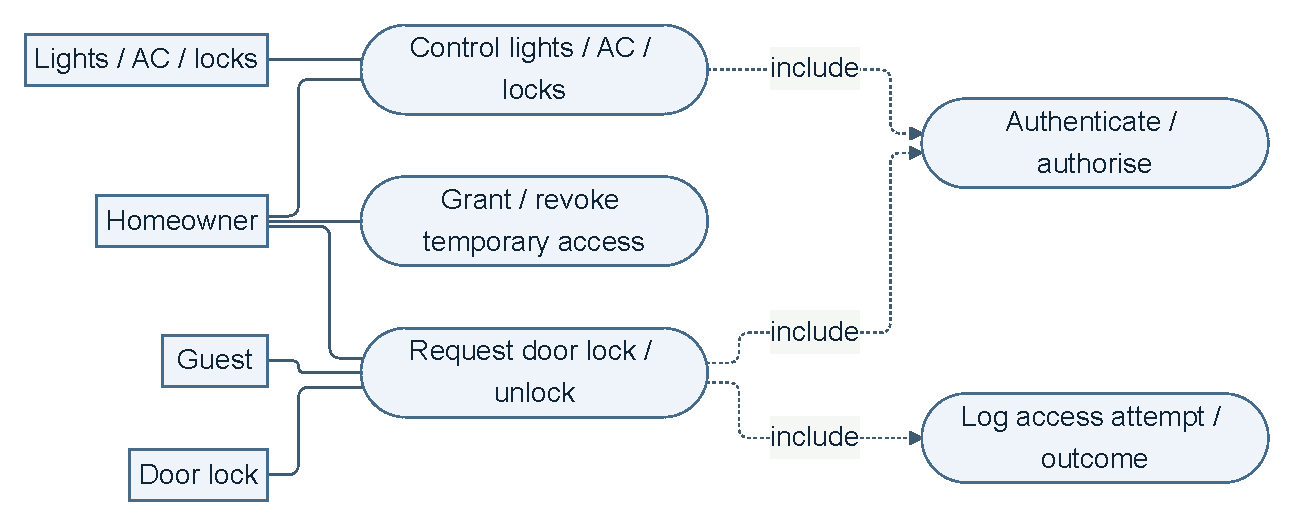
\includegraphics[width=364.32pt]{images/fig-079-user.pdf}
\captionof{figure}{Q1 --- Use cases (25 marks) --- device control and access}\end{minipage}\par\smallskip


\par\smallskip\noindent\begin{minipage}{\linewidth}\centering
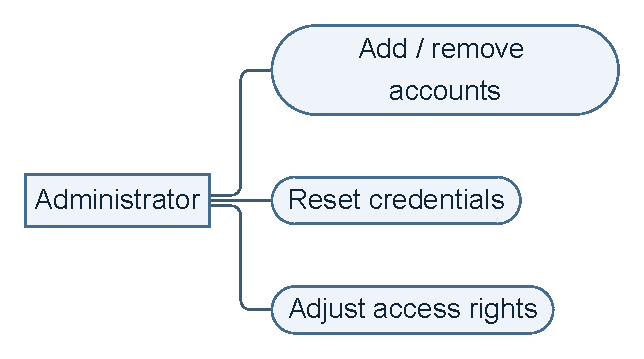
\includegraphics[width=181.28pt]{images/fig-079-admin.pdf}
\captionof{figure}{Q1 --- Use cases (25 marks) --- account administration}\end{minipage}\par\smallskip



\par\smallskip\noindent\begin{minipage}{\linewidth}\centering
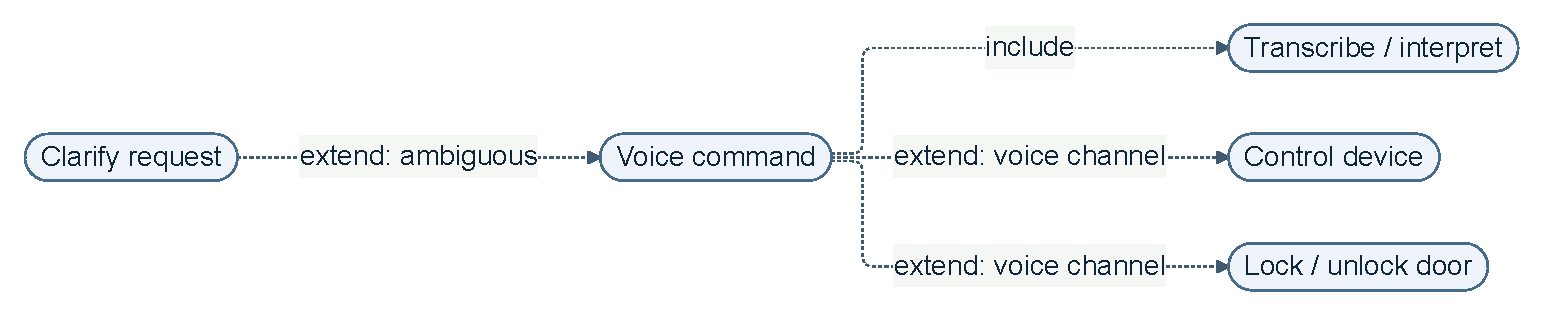
\includegraphics[width=434.72pt]{images/fig-079-voice.pdf}
\captionof{figure}{Q1 --- Use cases (25 marks) --- optional voice channel and clarification}\end{minipage}\par\smallskip

\begin{studycolumns}
\vspace{0pt}




Authorisation includes a guest's door-specific grant, revocation status and current time. Do not generalise Administrator from Homeowner or give administrators device-control associations. An owner-granted access period is not a one-time login token or permission for every door. Both permitted and denied guest attempts must reach the log.

\textbf{(b) Use case: Guest Door Access.} Primary actor: Guest. Supporting actor: Door Lock; voice interface if selected. Preconditions: guest identity can be authenticated; door and guest grant can be identified. Do \textbf{not} require ``current time is valid'' as the only precondition if the description must cover out-of-window denial. Flow: guest requests lock/\allowbreak{}unlock for a specific door through app or voice; system interprets/\allowbreak{}clarifies the request as needed; authenticate guest; check action, door, grant, revocation and time; execute permitted command through the lock interface; record request/\allowbreak{}time/\allowbreak{}outcome and show confirmation. Alternatives: no grant, revoked grant, wrong door or outside period, deny and log; ambiguous command, clarify without unlocking; device failure, log failure and report it rather than claiming success. A voice utterance alone is not proof of identity.

\needspace{4\baselineskip}
\subsection*{Q2 --- Access states, voice activity and process (25 marks)}
\sectionlabel{h-q2--access-states-voice-activity-and-process-25-marks}
\textbf{(a) Temporary guest access-controller state machine (4). (b) Guest voice-unlock activity/\allowbreak{}swimlanes (8). (c) Waterfall/\allowbreak{}Agile comparison: flexibility, customer involvement, delivery and one advantage each (5). (d) Two sprint advantages and two challenges, with examples (8).}


\textbf{(a)} Model one guest--door grant. \textbf{Assumption:} a time window is half-open \code{[start,\allowbreak{}end)}; the paper requires a strict window but does not specify endpoint inclusion. Agree the exact policy before implementation/\allowbreak{}testing.
\end{studycolumns}


\par\smallskip\noindent\begin{minipage}{\linewidth}\centering
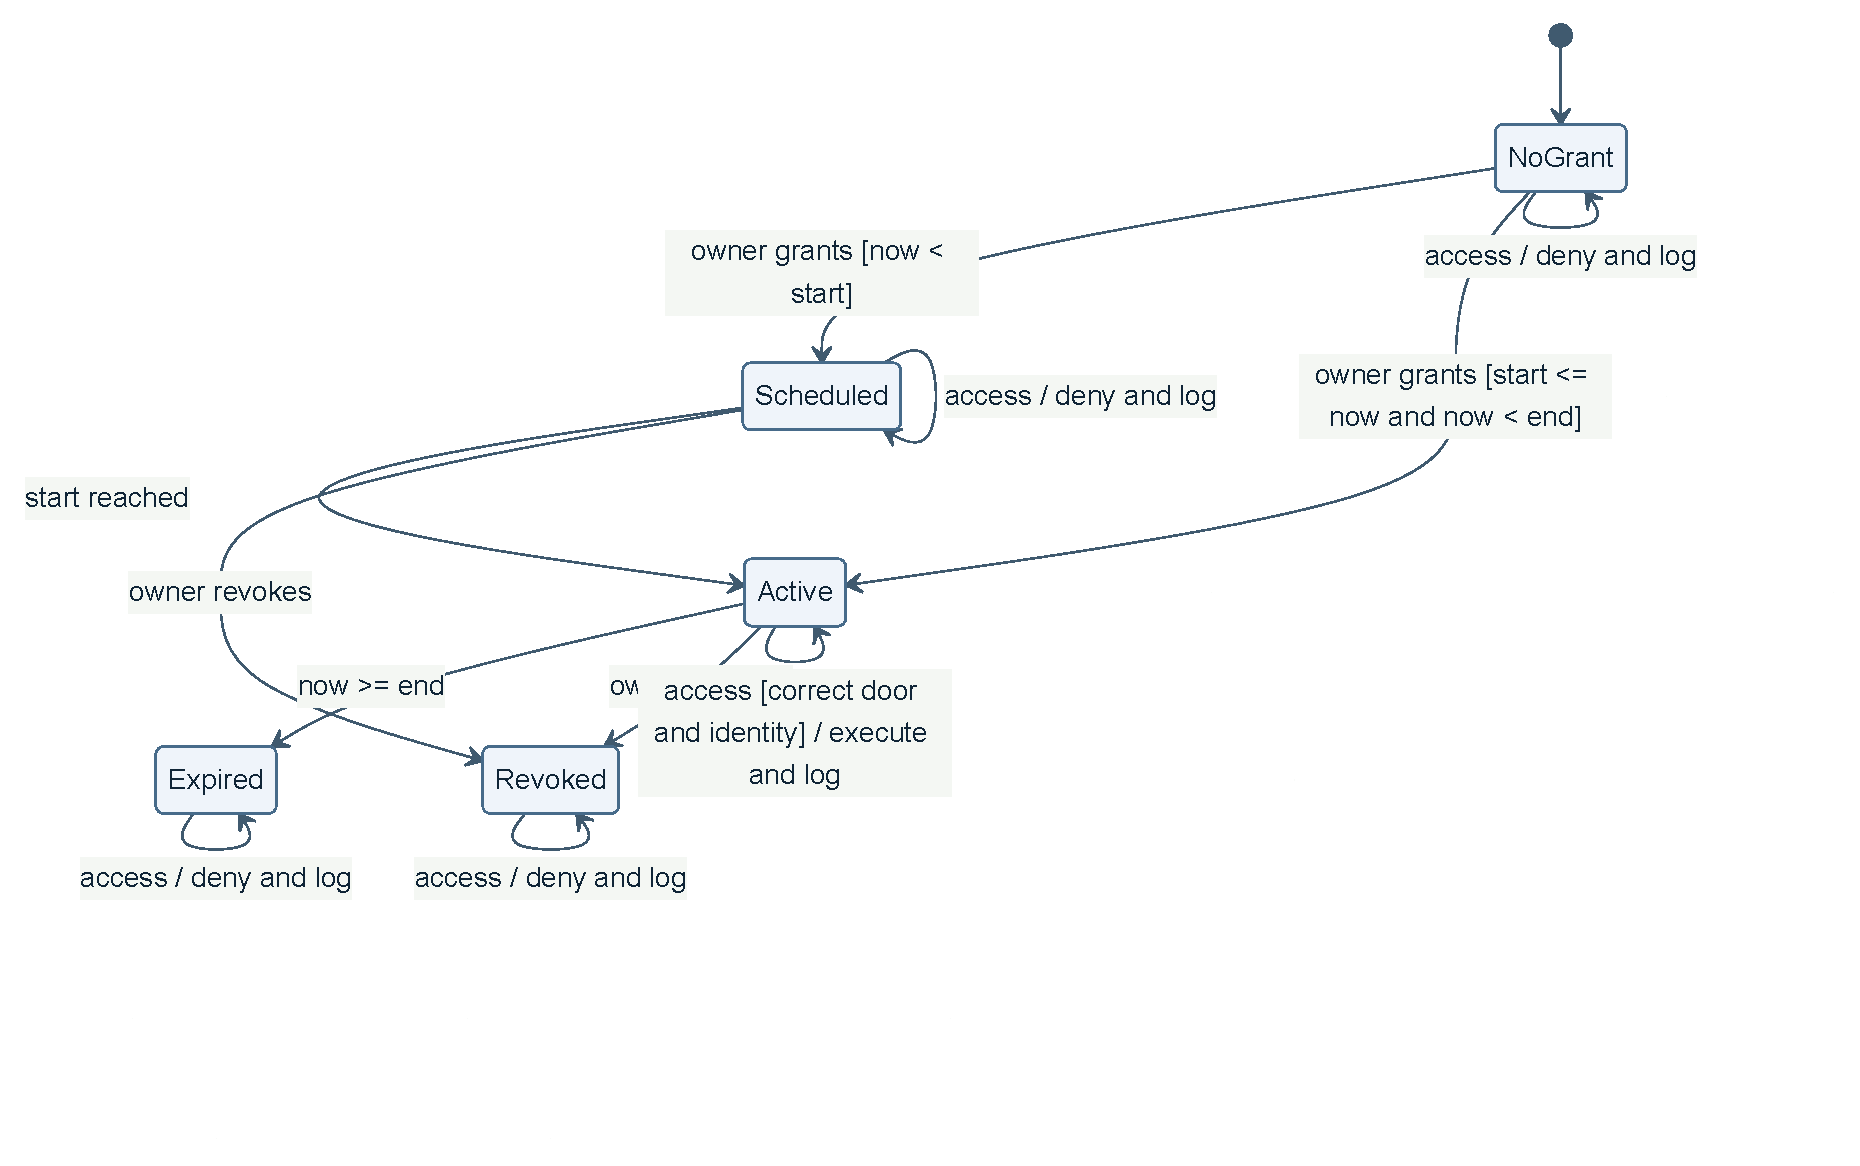
\includegraphics[width=446.65pt]{images/fig-080.pdf}
\captionof{figure}{Q2 --- Access states, voice activity and process (25 marks)}\end{minipage}\par\smallskip


A new grant can create a fresh controller/\allowbreak{}grant instance. A command arriving late must recheck time before execution; being previously Active is not enough.





\textbf{(b)}


\par\smallskip\noindent\begin{minipage}{\linewidth}\centering
{\scriptsize\textbf{Interpret and clarify}}\par\smallskip
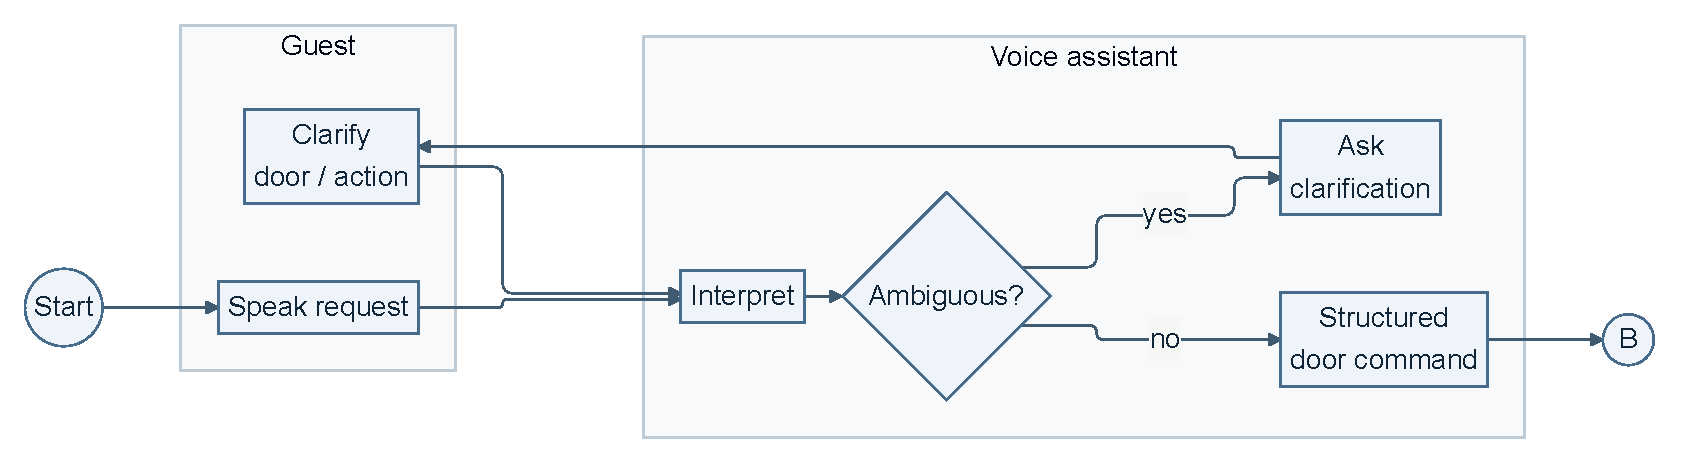
\includegraphics[width=430.00pt]{images/fig-081-a.pdf}\par\smallskip
{\scriptsize\textbf{Enforce policy, operate lock, log result}}\par\smallskip
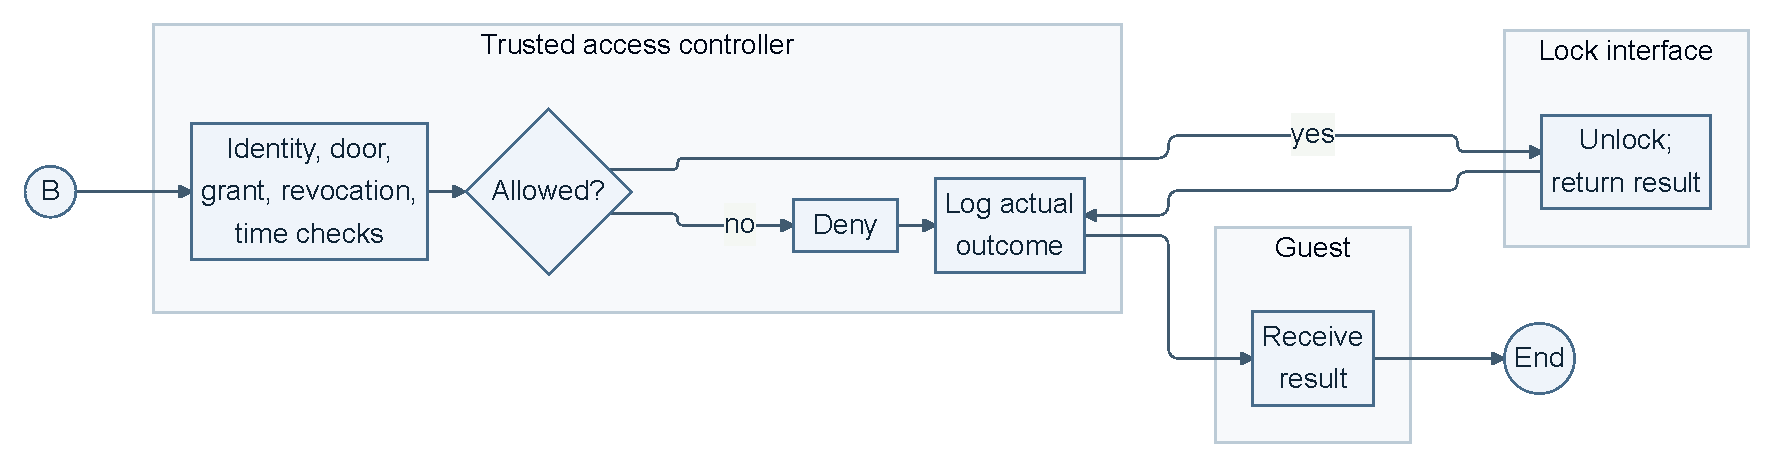
\includegraphics[width=454.00pt]{images/fig-081-b.pdf}\par\smallskip
\captionof{figure}{Q2 --- Access states, voice activity and process (25 marks)}\end{minipage}\par\smallskip

\begin{studycolumns}
\vspace{0pt}










LLM output proposes an action; deterministic access rules decide whether it can occur. Failure to interpret/\allowbreak{}authenticate must not unlock the door.

\textbf{(c)} Compare flexibility, customer involvement, delivery and strengths using \hyperref[answer-waterfall]{W, p.\ \pageref{answer-waterfall}}. Apply the comparison to owner/guest/device access increments.

\textbf{(d)} Apply \hyperref[answer-scrum]{S, p.\ \pageref{answer-scrum}}. Two benefits: owner feedback on voice clarification; visible tested guest-access increments. Two challenges: oversized voice/device work (split/spike) and hardware/urgent-change dependencies (doubles, early integration and backlog negotiation).

\needspace{4\baselineskip}
\subsection*{Q3 --- Smart-home architecture and pattern judgement (25 marks)}
\sectionlabel{h-q3--smart-home-architecture-and-pattern-judgement-25-marks}
\textbf{(a)(i) Architecture/\allowbreak{}detailed classes (8); (ii) one NFR and alternative architecture (8). (b)(i) Combined-pattern scenario/\allowbreak{}classes (6); (ii) evaluate the cost of pattern overuse (3).}


\textbf{(a)(i)} Use layered channel interfaces, application command control, domain access policy and device gateways. Both app and voice requests reach the same trusted policy before actuation.
\end{studycolumns}


\par\smallskip\noindent\begin{minipage}{\linewidth}\centering
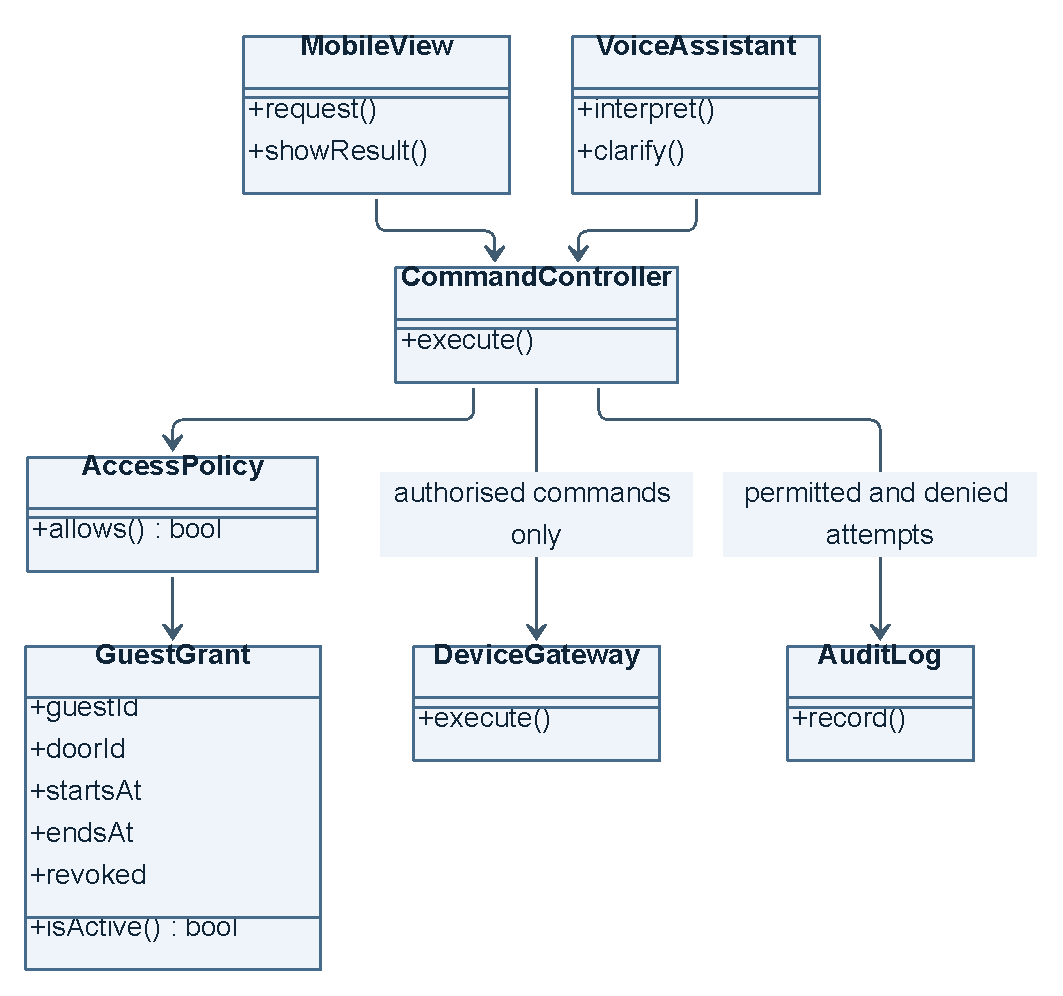
\includegraphics[width=298.90pt]{images/fig-082.pdf}
\captionof{figure}{Q3 --- Smart-home architecture and pattern judgement (25 marks)}\end{minipage}\par\smallskip




\textbf{(a)(ii)} Choose \textbf{security}, explicitly required by authentication, role separation and time-limited door grants. An alternative \textbf{client--server architecture with a security Facade/\allowbreak{}reference gate} treats app and LLM processing as untrusted input channels. Only a trusted server-side access service can invoke device gateways. Account administration uses a separate authorised API and does not confer device-control rights.




\par\smallskip\noindent\begin{minipage}{\linewidth}\centering
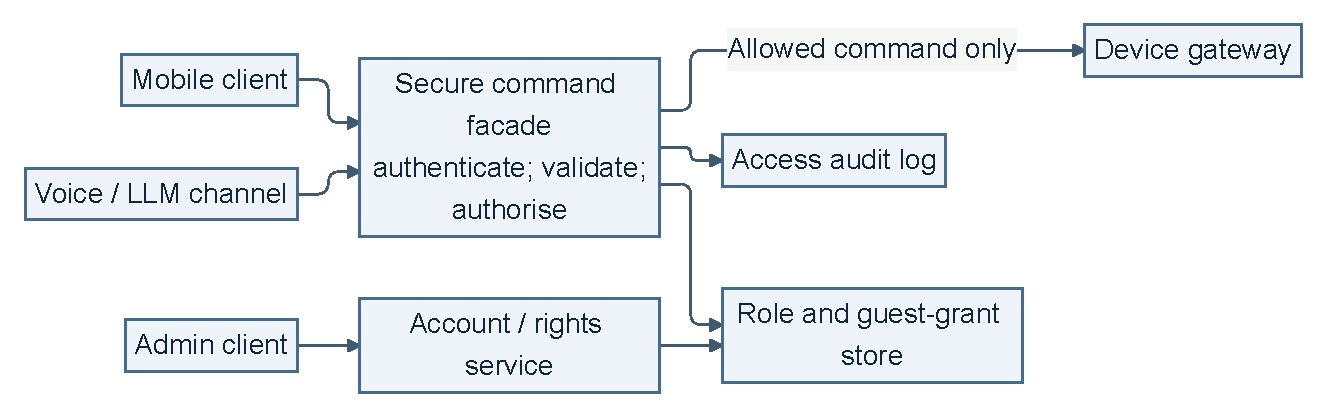
\includegraphics[width=374.00pt]{images/fig-083.pdf}
\captionof{figure}{Q3 --- Smart-home architecture and pattern judgement (25 marks)}\end{minipage}\par\smallskip

\begin{studycolumns}
\vspace{0pt}



Compared with policy spread among clients, a central gate prevents channel-specific bypasses and keeps one authoritative time/\allowbreak{}grant check. It introduces connectivity/\allowbreak{}availability concerns that require explicit failure behaviour; door access must not silently bypass checks when the policy service fails. This is a deployment/\allowbreak{}trust-boundary alternative compatible with layered internals.

\textbf{(b)(i)} Combine Strategy for role-specific permission policies with Simple Factory for selecting the policy from the \textbf{authenticated role}, never an LLM-supplied role string.





\textbf{Class diagram:} use \hyperref[shared-pattern]{P, p.\ \pageref{shared-pattern}}. Context = \code{Access\allowbreak{}Service}; Strategy = \code{Access\allowbreak{}Policy}; Factory = \code{Policy\allowbreak{}Factory}. Concrete strategies: \code{Owner\allowbreak{}Policy}, \code{Guest\allowbreak{}Policy}, \code{Administrator\allowbreak{}Policy}. Interface/concrete operations: \code{allows()}. Select from the authenticated role, never an LLM role string. Guest checks door/time/revocation; Administrator denies device control.







\textbf{(b)(ii)} Agree: use \hyperref[answer-pattern-cost]{C, p.\ \pageref{answer-pattern-cost}}. Trivial access rules may need only a policy table; introduce patterns for actual policy variation/coupling.

\needspace{4\baselineskip}
\subsection*{Q4 --- User inputs and automation (25 marks)}
\sectionlabel{h-q4--user-inputs-and-automation-25-marks}
\textbf{(a)(i) Derive ECs for Name, Phone Number, Access Expiry Date and Type of the User (4). (ii) Give on/\allowbreak{}below/\allowbreak{}above boundary values (4). (iii) Design defensive tests (5).}


\textbf{Input interpretation.} Name must be ASCII; Phone Number is a 8-digit integer; Access Expiry Date is between 2025 and 2030; Type of the User is one of \code{Administrator}, \code{Owner}, \code{Guest}, \code{One Time User}. Assume a positive 8-digit numeric value (not a string whose leading zeroes count as digits), inclusive complete calendar years, and one-day date resolution. These interpretations are stated because the brief does not specify parsing details. Do not invent an ASCII-field length limit.

\textbf{(i) Equivalence classes:}
\end{studycolumns}


{\fontsize{8.5}{9.8}\selectfont
\begin{longtable}{L{\dimexpr 0.21857\linewidth-5.25pt\relax}L{\dimexpr 0.33977\linewidth-8.15pt\relax}L{\dimexpr 0.44166\linewidth-10.60pt\relax}}
\toprule
\rowcolor{ice}\textbf{Field} & \textbf{Valid EC} & \textbf{Invalid ECs} \\
\midrule\endfirsthead
\toprule\rowcolor{ice}\textbf{Field} & \textbf{Valid EC} & \textbf{Invalid ECs} \\
\midrule\endhead
\multicolumn{3}{r}{\scriptsize Continued on next page}\\\endfoot
\bottomrule\endlastfoot
Name & ASCII text & Text containing non-ASCII characters \\
Phone Number & Integer 10000000\ldots{}99999999 & Integer below 10000000; integer above 99999999; malformed/\allowbreak{}non-integer input at the input boundary \\
Access Expiry Date & Real calendar date 2025-01-01\ldots{}2030-12-31 & Real date before 2025-01-01; real date after 2030-12-31; malformed/\allowbreak{}nonexistent date \\
Type of the User & One EC containing \{Administrator, Owner, Guest, One Time User\} & Any unlisted value \\
\end{longtable}
}

The category set is \textbf{one valid EC}, although testing all its few members is useful. No empty-string prohibition or printable-only ASCII restriction is supplied; clarify those separately instead of asserting an invented oracle.

\textbf{(ii) Boundary triplets:}




{\fontsize{8.5}{9.8}\selectfont
\begin{longtable}{L{\dimexpr 0.27995\linewidth-8.96pt\relax}L{\dimexpr 0.23807\linewidth-7.62pt\relax}L{\dimexpr 0.24099\linewidth-7.71pt\relax}L{\dimexpr 0.24099\linewidth-7.71pt\relax}}
\toprule
\rowcolor{ice}\textbf{Field /\allowbreak{} boundary} & \textbf{Just below} & \textbf{On boundary} & \textbf{Just above} \\
\midrule\endfirsthead
\toprule\rowcolor{ice}\textbf{Field /\allowbreak{} boundary} & \textbf{Just below} & \textbf{On boundary} & \textbf{Just above} \\
\midrule\endhead
\multicolumn{4}{r}{\scriptsize Continued on next page}\\\endfoot
\bottomrule\endlastfoot
Phone Number: minimum & 9999999 (reject) & 10000000 (accept) & 10000001 (accept) \\
Phone Number: maximum & 99999998 (accept) & 99999999 (accept) & 100000000 (reject) \\
Access Expiry Date: earliest & 2024-12-31 (reject) & 2025-01-01 (accept) & 2025-01-02 (accept) \\
Access Expiry Date: latest & 2030-12-30 (accept) & 2030-12-31 (accept) & 2031-01-01 (reject) \\
\end{longtable}
}

ASCII membership and unordered categories have no specified application-level ordered boundary. Malformed values are additional EC tests, not numeric/\allowbreak{}date neighbours.

\textbf{(iii) Defensive suite.} Use the common testing conventions below; valid rows combine boundaries, invalid rows isolate one field. The full boundary suite is retained.




{\fontsize{8.5}{9.8}\selectfont
\begin{longtable}{L{\dimexpr 0.16951\linewidth-6.78pt\relax}L{\dimexpr 0.16951\linewidth-6.78pt\relax}L{\dimexpr 0.17251\linewidth-6.90pt\relax}L{\dimexpr 0.17980\linewidth-7.19pt\relax}L{\dimexpr 0.30866\linewidth-12.35pt\relax}}
\toprule
\rowcolor{ice}\textbf{Name} & \textbf{Phone Number} & \textbf{Access Expiry Date} & \textbf{Type of the User} & \textbf{Expected /\allowbreak{} purpose} \\
\midrule\endfirsthead
\toprule\rowcolor{ice}\textbf{Name} & \textbf{Phone Number} & \textbf{Access Expiry Date} & \textbf{Type of the User} & \textbf{Expected /\allowbreak{} purpose} \\
\midrule\endhead
\multicolumn{5}{r}{\scriptsize Continued on next page}\\\endfoot
\bottomrule\endlastfoot
\code{Alex} & \code{10000000} & \code{2025-\allowbreak{}01-\allowbreak{}01} & \code{Administrator} & Accept --- valid boundaries /\allowbreak{} category coverage \\
\code{Alex} & \code{10000001} & \code{2025-\allowbreak{}01-\allowbreak{}02} & \code{Owner} & Accept --- valid boundaries /\allowbreak{} category coverage \\
\code{Alex} & \code{99999998} & \code{2030-\allowbreak{}12-\allowbreak{}30} & \code{Guest} & Accept --- valid boundaries /\allowbreak{} category coverage \\
\code{Alex} & \code{99999999} & \code{2030-\allowbreak{}12-\allowbreak{}31} & \code{One Time User} & Accept --- valid boundaries /\allowbreak{} category coverage \\
\code{Alex} & \code{54999999} & \code{2027-\allowbreak{}07-\allowbreak{}01} & \code{Administrator} & Accept --- interior baseline /\allowbreak{} category coverage \\
\code{caf\'{e}} & \code{54999999} & \code{2027-\allowbreak{}07-\allowbreak{}01} & \code{Administrator} & Reject --- non-ASCII Name \\
\code{Alex} & \code{9999999} & \code{2027-\allowbreak{}07-\allowbreak{}01} & \code{Administrator} & Reject --- Phone Number below minimum \\
\code{Alex} & \code{100000000} & \code{2027-\allowbreak{}07-\allowbreak{}01} & \code{Administrator} & Reject --- Phone Number above maximum \\
\code{Alex} & \code{54999999} & \code{2024-\allowbreak{}12-\allowbreak{}31} & \code{Administrator} & Reject --- Access Expiry Date below minimum \\
\code{Alex} & \code{54999999} & \code{2031-\allowbreak{}01-\allowbreak{}01} & \code{Administrator} & Reject --- Access Expiry Date above maximum \\
\code{Alex} & \code{54999999} & \code{2027-\allowbreak{}07-\allowbreak{}01} & \code{Unknown} & Reject --- unlisted Type of the User \\
\code{Alex} & \code{12x} & \code{2027-\allowbreak{}07-\allowbreak{}01} & \code{Administrator} & Reject --- malformed integer; extra defensive case \\
\code{Alex} & \code{54999999} & \code{2025-\allowbreak{}02-\allowbreak{}30} & \code{Administrator} & Reject --- nonexistent calendar date; extra defensive case \\
\end{longtable}
}

\begin{studycolumns}
\vspace{0pt}

The Q4 category \code{One Time User} is valid for this input question, although Appendix A does not define that role's device permissions. Do not invent its access policy from the category name.

\textbf{(b) How can LLMs assist automated testing? (4). (c) At least four challenges of fully automated development (8).}


\textbf{(b)} Use requirements and code context to propose tests, fixtures, boundary cases and automation scripts; run them through a real test runner and report actual results. Generate guest-access cases for wrong door, revocation and exact time edges, and validate expected results against the agreed policy. Review generated code/\allowbreak{}oracles and measure meaningful coverage. An LLM's claim that a test passed is not execution evidence; voice-language tests also need representative ambiguous/\allowbreak{}adversarial requests and repeatability controls.

\textbf{(c)} Four challenges with consequences: \textbf{ambiguous/\allowbreak{}incomplete requirements} require stakeholder clarification, otherwise correct-looking code solves the wrong problem; \textbf{incorrect or nondeterministic generation} can introduce defects/\allowbreak{}security flaws, requiring independent execution and review; \textbf{integration/\allowbreak{}context limits} make existing interfaces, hardware behaviour and cross-component invariants hard to preserve; \textbf{validation and accountability} require trusted oracles, quality-attribute evidence and responsibility for consequential decisions. Maintenance adds further difficulty because changes must preserve compatibility, intent and operational safety across versions. In this case, a plausible voice response cannot establish that a physical door was correctly authorised or operated.
\end{studycolumns}

\par\Needspace{120pt}\medskip
\section*{Paper 8: AY2025/\allowbreak{}26 Semester 2 --- Restaurant Recommendation System}\label{paper-2526-s2}
\phantomsection\addcontentsline{toc}{section}{Paper 8: AY2025/26 Semester 2 --- Restaurant Recommendation System}\markboth{AY2025/26 S2}{}
\sectionlabel{h-192-ay202526-semester-2--restaurant-recommendation-system}
\textbf{Source:} \href{run:/Users/bryangoh/Work/ntu-cs/sc2006/pyps/SC2006\_AY2526\_S2\_Questions.pdf}{Question paper}, Q1--Q4 on PDF pp. 1--3; Appendix A on p. 4.




\begin{studycolumns}
\vspace{0pt}
\textbf{Case facts.} Anonymous users converse with an LLM about food preferences. Conversation ends after ten user/\allowbreak{}assistant message pairs or an earlier Finished action. The same LLM then returns JSON containing up to five tags from a fixed set of twenty. Invalid JSON, out-of-set tags or more than five tags produces an error and a restart invitation. With valid tags, user provides postcode and integer travel radius; recommendations stay within radius and sort by decreasing count of matching tags. Clicking a restaurant website records preferences and selection. Administrators authenticate to maintain restaurant entries and view selection logs.

\needspace{4\baselineskip}
\subsection*{Q1 --- Use cases and JSON-check activity (25 marks)}
\sectionlabel{h-q1--use-cases-and-json-check-activity-25-marks}
\textbf{(a) Actors/\allowbreak{}use cases/\allowbreak{}relationships (18). (b) Activity/\allowbreak{}swimlane diagram for checking JSON output (7).}


\textbf{(a)} Actors: Anonymous User, Administrator, and external LLM Service if externally hosted (explicitly the deployment considered in Q3(c)). The database and validation function are internal components. A restaurant website need not be a supporting actor merely because the browser follows its link.
\end{studycolumns}


\par\smallskip\noindent\begin{minipage}{\linewidth}\centering
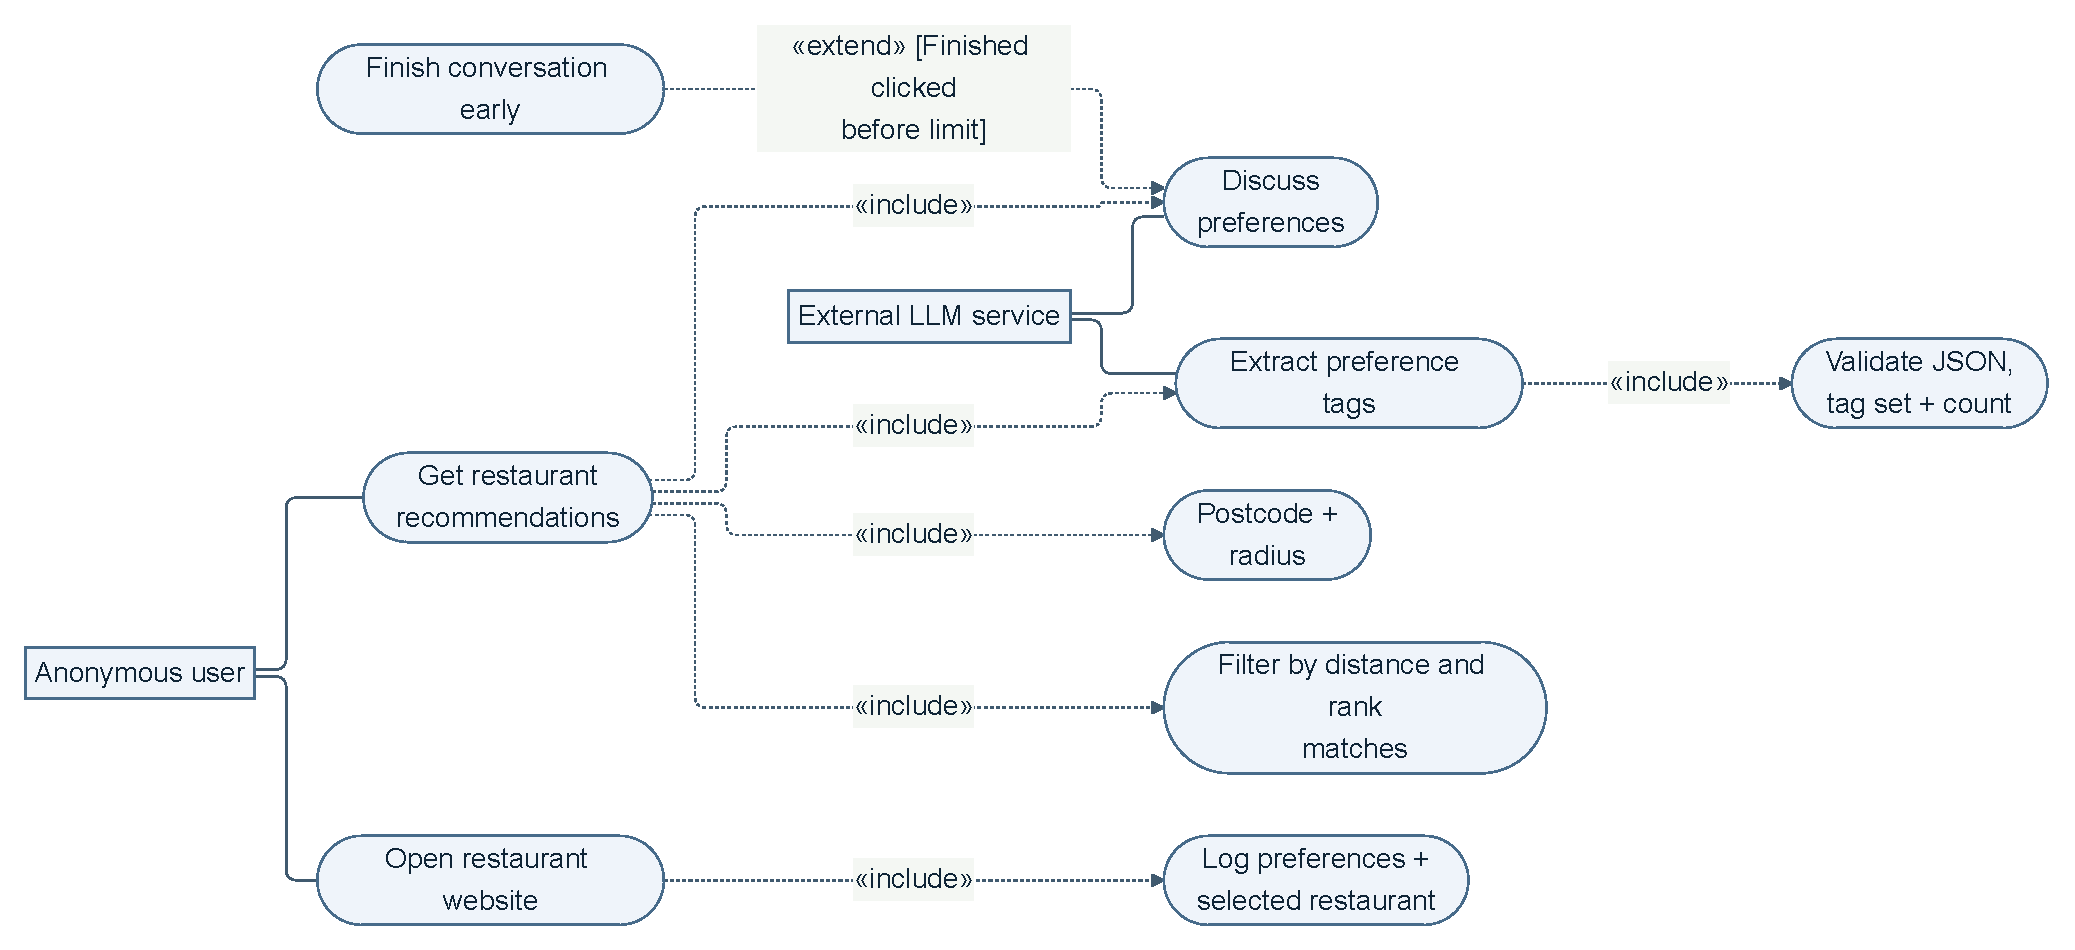
\includegraphics[width=514.00pt]{images/fig-085-user.pdf}
\captionof{figure}{Q1 --- Use cases and JSON-check activity (25 marks) --- anonymous user and supporting LLM view}\end{minipage}\par\smallskip








\par\smallskip\noindent\begin{minipage}{\linewidth}\centering
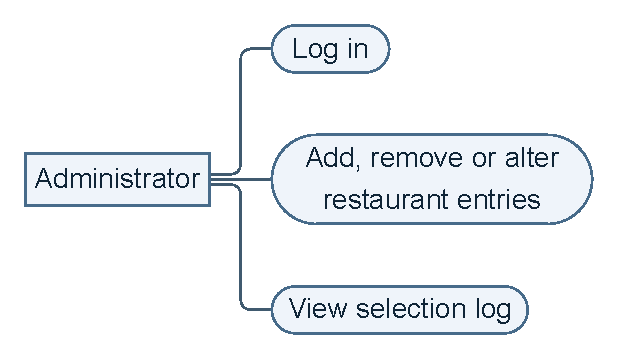
\includegraphics[width=173.80pt]{images/fig-085-admin.pdf}
\captionof{figure}{Q1 --- Use cases and JSON-check activity (25 marks) --- administrator view}\end{minipage}\par\smallskip

\begin{studycolumns}
\vspace{0pt}



Protected administrator actions require authentication; anonymous recommendations do not. Early finish is optional; reaching ten completed pairs also ends the conversation. Location/\allowbreak{}ranking steps belong to the successful flow; validation failure terminates that attempt before them. Recording a selection happens on a website click, not automatically for every displayed restaurant.

\textbf{(b)} \textbf{Schema assumption:} the LLM contract represents tags as a JSON array of strings (or an agreed object field holding that array). JSON validity alone does not ensure that the parsed shape is usable as a tag list.
\end{studycolumns}


\par\smallskip\noindent\begin{minipage}{\linewidth}\centering
{\scriptsize\textbf{Validate JSON, shape, count and fixed tag set}}\par\smallskip
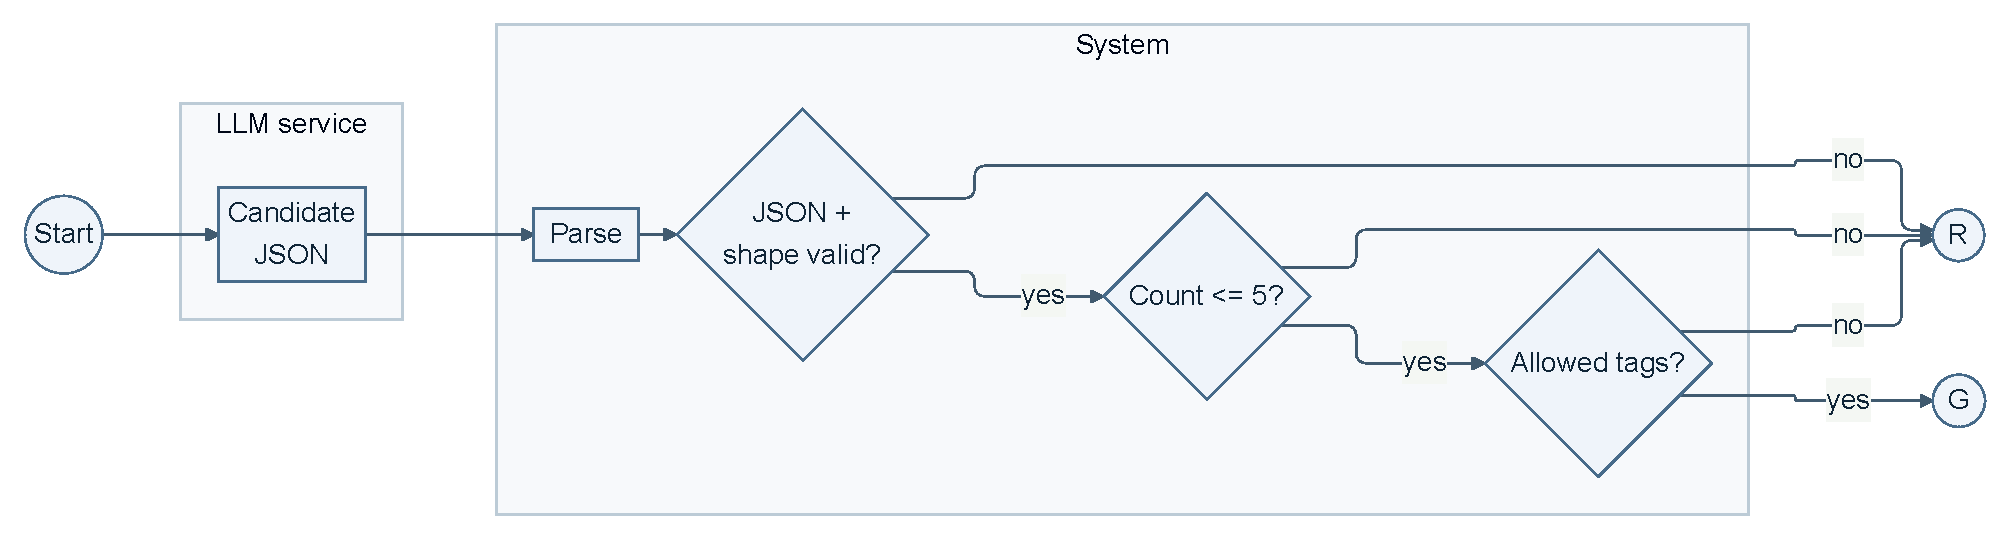
\includegraphics[width=514.00pt]{images/fig-086-a.pdf}\par\smallskip
{\scriptsize\textbf{Accept location input or offer restart}}\par\smallskip
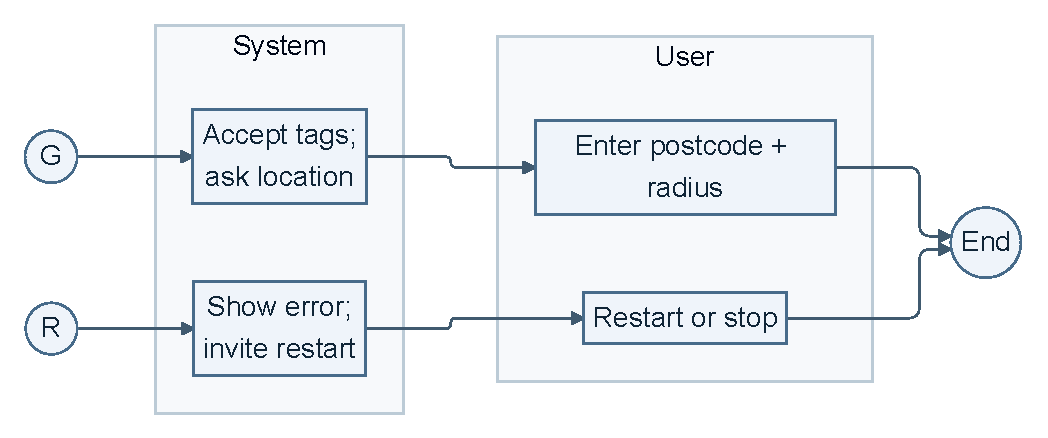
\includegraphics[width=268.00pt]{images/fig-086-b.pdf}\par\smallskip
\captionof{figure}{Q1 --- Use cases and JSON-check activity (25 marks) --- G = accepted tags; R = rejected candidate.}\end{minipage}\par\smallskip

\begin{studycolumns}
\vspace{0pt}




``Up to five'' supplies no minimum-one rule: do not reject an empty tag list unless a separate requirement establishes that rule. Duplicate-tag handling is unspecified; do not silently add a rejection requirement. Count entries before any optional deduplication so a six-entry response cannot evade the stated limit.

\needspace{4\baselineskip}
\subsection*{Q2 --- Recommendation classes, conversation states and Scrum (25 marks)}
\sectionlabel{h-q2--recommendation-classes-conversation-states-and-scrum-25-marks}
\textbf{(a) Recommendation-generation conceptual classes/\allowbreak{}stereotypes (8). (b) Conversation state machine (6). (c) Waterfall versus Agile when the tag set changes (5). (d) Two causes/\allowbreak{}remedies for frequently overrun sprints (6).}


\textbf{(a)}
\end{studycolumns}


\par\smallskip\noindent\begin{minipage}{\linewidth}\centering
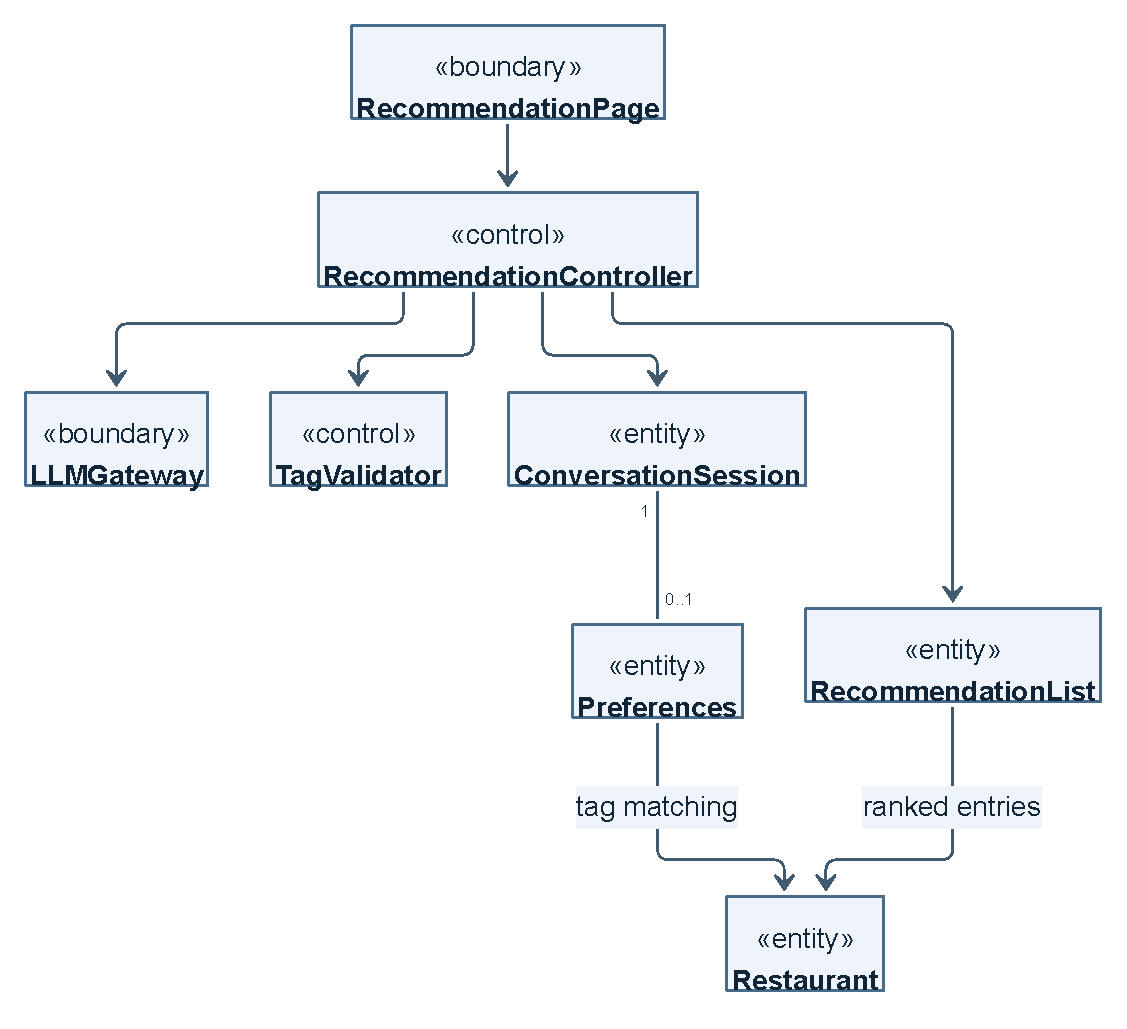
\includegraphics[width=306.81pt]{images/fig-087.pdf}
\captionof{figure}{Q2 --- Recommendation classes, conversation states and Scrum (25 marks)}\end{minipage}\par\smallskip



Postcode/\allowbreak{}radius belong to the recommendation request; preferences contain validated tags. No registered-user entity is required for anonymous use.

\textbf{(b)} Count \textbf{completed user/\allowbreak{}assistant pairs}, not individual messages. The limit is ten of each, not ten combined.




\par\smallskip\noindent\begin{minipage}{\linewidth}\centering
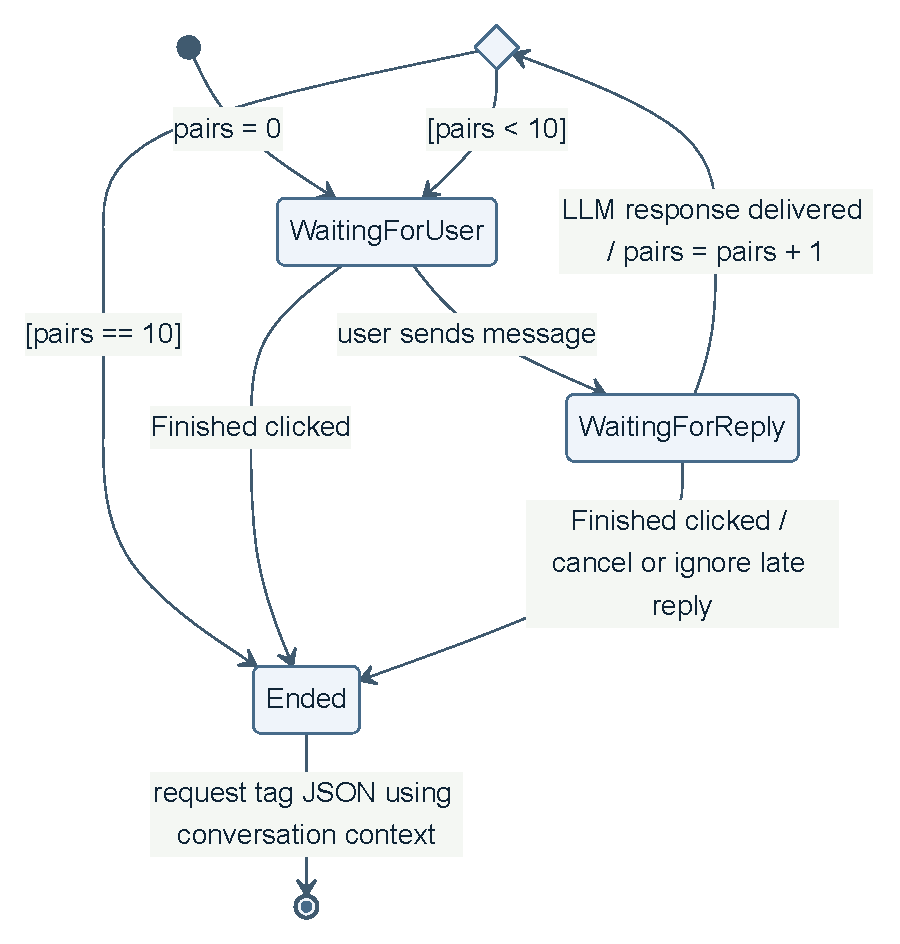
\includegraphics[width=253.00pt]{images/fig-088.pdf}
\captionof{figure}{Q2 --- Recommendation classes, conversation states and Scrum (25 marks)}\end{minipage}\par\smallskip

\begin{studycolumns}
\vspace{0pt}



Handling Finished while a reply is pending is a stated design choice; it must not reopen the ended conversation when a late reply arrives. Restart after invalid tag JSON starts a fresh session. JSON validation/\allowbreak{}recommendation are subsequent components, not extra conversation messages.

\textbf{(c)} Apply \hyperref[answer-waterfall]{W, p.\ \pageref{answer-waterfall}}. A tag-set change affects prompts, validators, restaurant data, UI and tests. Version/configure the vocabulary consistently; changing only the prompt is insufficient.

\textbf{(d)} Use \hyperref[answer-scrum]{S, p.\ \pageref{answer-scrum}}. Oversized/optimistic stories: split and select less work using actual capacity. Hidden LLM/API/integration or support work: investigate early, use doubles and budget support capacity. Replan unfinished work.

\end{studycolumns}
\Needspace{85pt}
\subsection*{Q3 --- Architecture and external LLM trade-offs (25 marks)}
\begin{studycolumns}
\sectionlabel{h-q3--architecture-and-external-llm-trade-offs-25-marks}
\textbf{(a) Architecture (3). (b) Detailed classes with attributes/\allowbreak{}methods (12). (c)(i) Two upsides/\allowbreak{}two downsides of self-hosting an LLM (4); (ii) two other responses to a hosted LLM advertising competitors (6).}


\textbf{(a)} Use client--server with layered application/\allowbreak{}domain services and an external LLM gateway. MVC can organise browser interaction: views display conversation/\allowbreak{}results, controllers accept inputs, and domain models/\allowbreak{}services hold conversation, tag-validation and recommendation rules. Keep the restaurant database, logging and administrator authorisation on the server; never trust unvalidated LLM output.

\textbf{(b)} Two views of one class model keep the diagram readable. \code{Session\allowbreak{}Controller} is the same class in both views; operations are shown in the view that uses them.
\end{studycolumns}


\par\smallskip\noindent\begin{minipage}{\linewidth}\centering
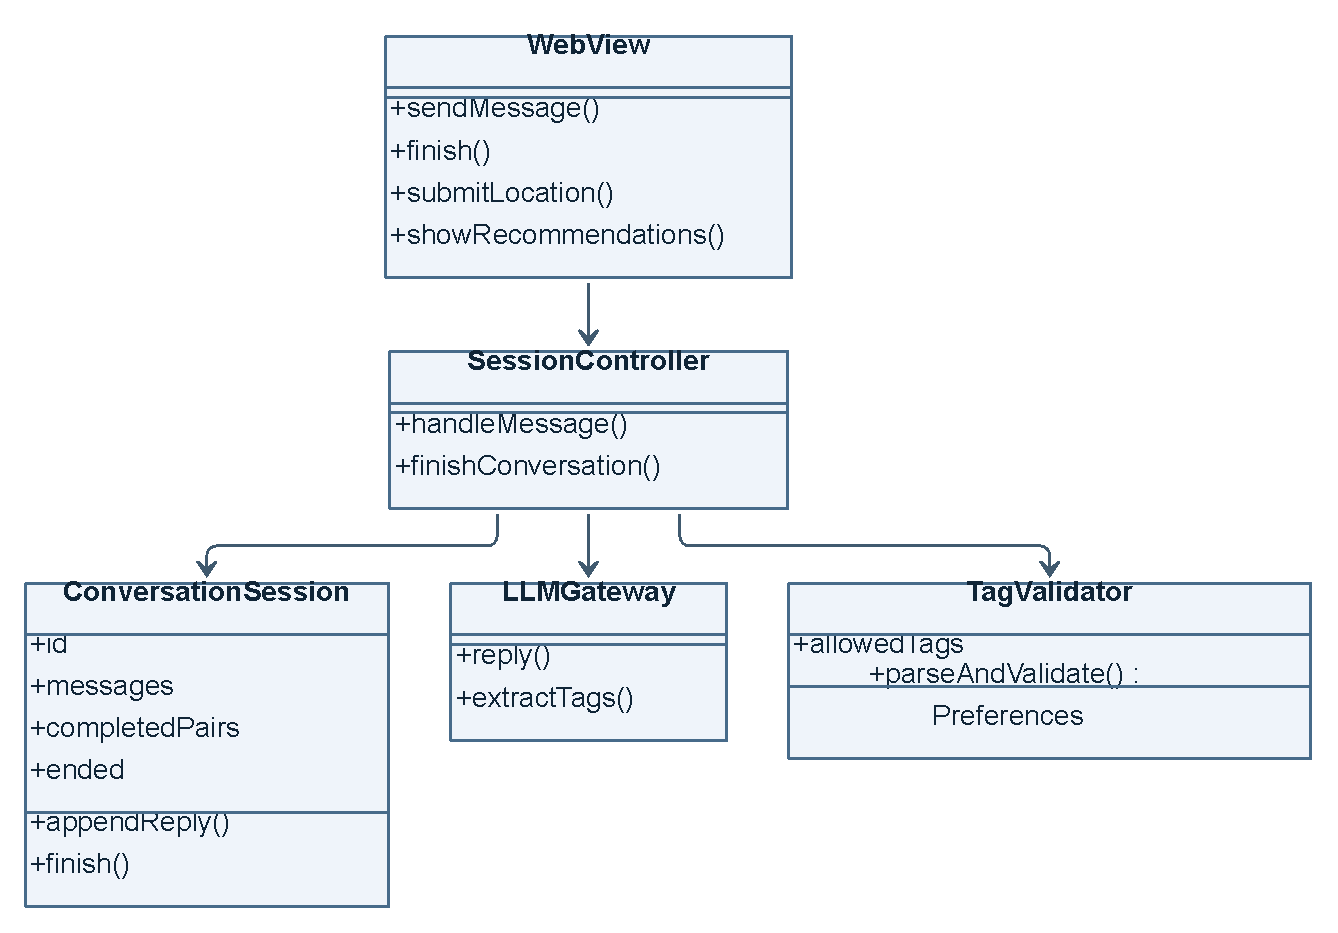
\includegraphics[width=376.64pt]{images/fig-089.pdf}
\captionof{figure}{Q3 --- Architecture and external LLM trade-offs (25 marks)}\end{minipage}\par\smallskip









\par\smallskip\noindent\begin{minipage}{\linewidth}\centering
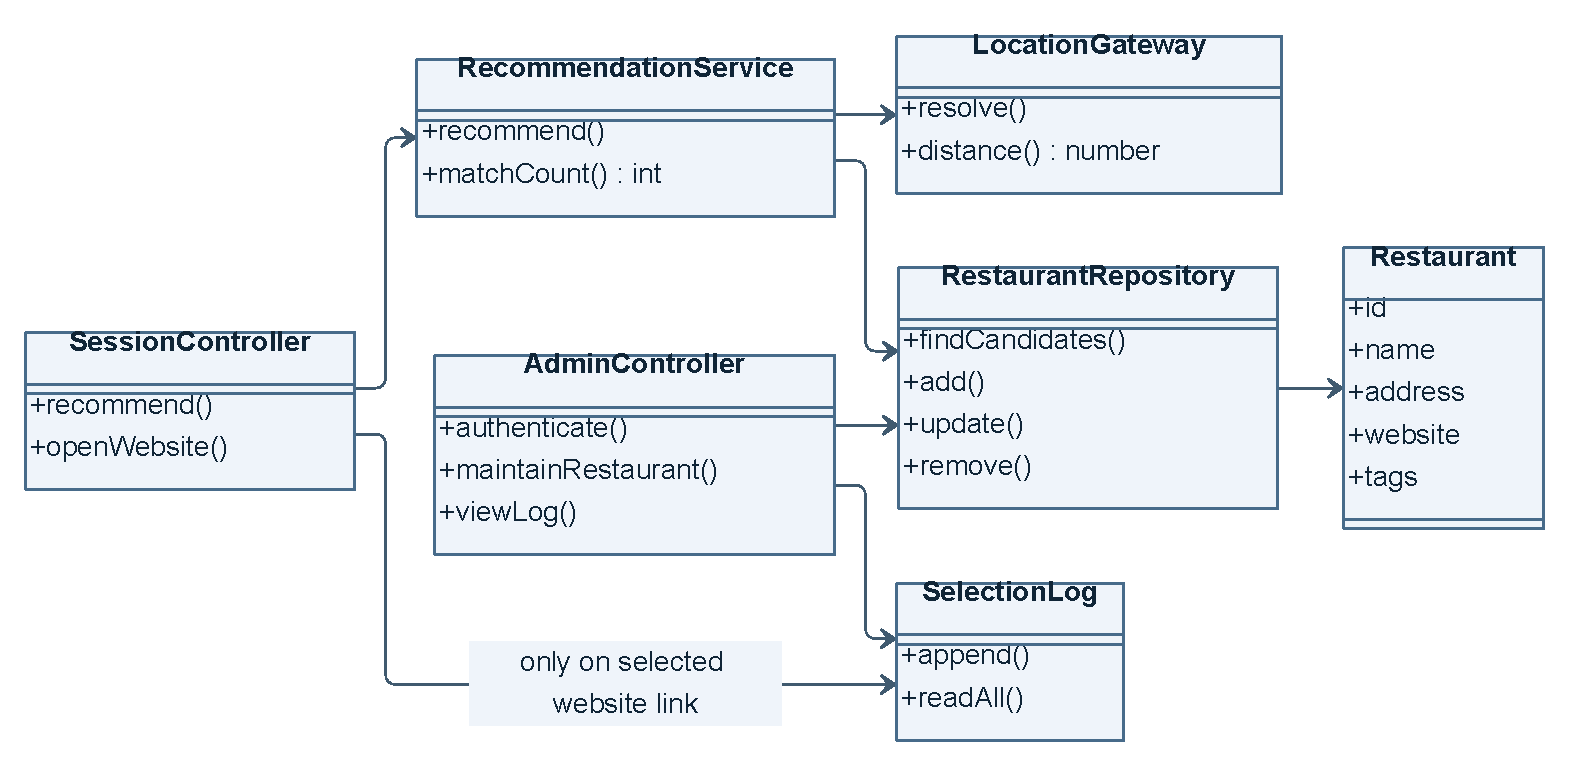
\includegraphics[width=441.76pt]{images/fig-090.pdf}
\captionof{figure}{Q3 --- Architecture and external LLM trade-offs (25 marks)}\end{minipage}\par\smallskip

\begin{studycolumns}
\vspace{0pt}





A server-side selection endpoint records the preferences/\allowbreak{}restaurant associated with that anonymous session, then redirects to the restaurant website. Domain algorithm: resolve location; retain restaurants with \code{distance \ensuremath{\leq} radius}; compute the number of matching preference tags; sort descending; display names and website links. Zero matches are not explicitly excluded. Tie ordering and distance calculation method are unspecified; declare any chosen policy. Location resolution is a proposed integration needed for distance calculation, distinct from Q4's initially format-only validator.

\textbf{(c)(i)} Self-hosting upsides: \textbf{control over model behaviour/\allowbreak{}version/\allowbreak{}customisation}, and \textbf{control over data handling with less dependence on a hosted provider's policies/\allowbreak{}availability}. Downsides: \textbf{compute/\allowbreak{}infrastructure cost}, and \textbf{operational/\allowbreak{}expertise burden} for serving, monitoring, updates, capacity and security. Self-hosting does not automatically deliver better accuracy or eliminate harmful outputs.

\textbf{(c)(ii)} Two approaches other than self-hosting:

\begin{enumerate}
\item \textbf{Switch to another externally hosted model/\allowbreak{}provider}, through the gateway, after testing against conversation and tag-extraction requirements. Establish service/\allowbreak{}content expectations and regression checks; avoid merely assuming every alternative behaves better.
\item \textbf{Add a server-side output-policy boundary.} Check user-visible replies for unwanted promotional content, block affected responses and request a constrained regeneration with bounded retries; provide a controlled error/\allowbreak{}fallback when checks fail. Keep tag extraction under strict structural/\allowbreak{}membership validation as well. A prompt instruction alone is not a reliable enforcement boundary, and valid JSON does not establish that freeform replies contain no advertising. Evaluate false positives/\allowbreak{}negatives and preserve the required conversation capability.
\end{enumerate}
\needspace{4\baselineskip}
\subsection*{Q4 --- Postcode/\allowbreak{}distance ECs, external API and internationalisation (25 marks)}
\sectionlabel{h-q4--postcodedistance-ecs-external-api-and-internationalisation-25-marks}
\textbf{Given:} \code{validate\allowbreak{}User\allowbreak{}Input(postcode,\allowbreak{} distance)} accepts a postcode string of six numerical digits and an integer distance from 0 to 100 km inclusive. \textbf{(a) ECs/\allowbreak{}assumptions (4). (b) Boundary triplets (4). (c) Defensive suite (8). (d)(i) EC changes when a public API confirms a real Singapore building (3); (ii) two complications for comprehensive tests (4). (e) Adaptation to multiple countries (2).}


\textbf{(a)} Assume ``numerical digits'' means ASCII \code{0}--\code{9}, retain leading zeroes, do not trim/\allowbreak{}coerce invalid inputs silently, and initially check \textbf{syntax only}, not real-building existence. The function contract already gives string/\allowbreak{}integer argument types; non-string/\allowbreak{}non-integer inputs are extra defensive-interface cases if the implementation permits them.
\end{studycolumns}


{\fontsize{8.5}{9.8}\selectfont
\begin{longtable}{L{\dimexpr 0.23363\linewidth-5.61pt\relax}L{\dimexpr 0.31394\linewidth-7.53pt\relax}L{\dimexpr 0.45243\linewidth-10.86pt\relax}}
\toprule
\rowcolor{ice}\textbf{Input} & \textbf{Valid EC} & \textbf{Invalid ECs} \\
\midrule\endfirsthead
\toprule\rowcolor{ice}\textbf{Input} & \textbf{Valid EC} & \textbf{Invalid ECs} \\
\midrule\endhead
\multicolumn{3}{r}{\scriptsize Continued on next page}\\\endfoot
\bottomrule\endlastfoot
Postcode & Exactly six ASCII digits: \code{[0-\allowbreak{}9]\{6\}} & Length other than six; length six with at least one non-digit (including non-ASCII digits) \\
Distance & Integer \code{0 \ensuremath{\leq} d \ensuremath{\leq} 100} & Integer \code{d < 0}; integer \code{d >\allowbreak{} 100} \\
\end{longtable}
}

\begin{studycolumns}
\vspace{0pt}

The postcode invalid classes are disjoint as defined. \code{000000} and \code{999999} are syntactically valid even if they do not identify buildings. Postcode is not an integer range from 100000 to 999999.

\textbf{(b)} Distance triplets: \code{\ensuremath{-}1,\allowbreak{} 0,\allowbreak{} 1} and \code{99,\allowbreak{} 100,\allowbreak{} 101}. Postcode \textbf{length} triplet: length \code{5,\allowbreak{} 6,\allowbreak{} 7}, e.g. \code{00000}, \code{000000}, \code{0000000}. Character membership is a discrete format rule; use a six-character string containing a letter/\allowbreak{}space rather than inventing an overall numeric postcode boundary.

\textbf{(c)} Reset/\allowbreak{}isolate each test. ``Accept'' means this validator returns acceptance; it does not promise that later geocoding/\allowbreak{}recommendation will succeed.
\end{studycolumns}


{\fontsize{8.5}{9.8}\selectfont
\begin{longtable}{L{\dimexpr 0.28067\linewidth-6.74pt\relax}L{\dimexpr 0.28067\linewidth-6.74pt\relax}L{\dimexpr 0.43866\linewidth-10.53pt\relax}}
\toprule
\rowcolor{ice}\textbf{Postcode string} & \textbf{Distance (km)} & \textbf{Expected /\allowbreak{} purpose} \\
\midrule\endfirsthead
\toprule\rowcolor{ice}\textbf{Postcode string} & \textbf{Distance (km)} & \textbf{Expected /\allowbreak{} purpose} \\
\midrule\endhead
\multicolumn{3}{r}{\scriptsize Continued on next page}\\\endfoot
\bottomrule\endlastfoot
\code{612345} & 50 & Accept --- baseline \\
\code{000000} & 50 & Accept --- leading zeroes, syntax only \\
\code{999999} & 50 & Accept --- six digits, syntax only \\
\code{612345} & 0 & Accept --- lower distance boundary \\
\code{612345} & 1 & Accept --- lower valid neighbour \\
\code{612345} & 99 & Accept --- upper valid neighbour \\
\code{612345} & 100 & Accept --- upper distance boundary \\
\code{612345} & \ensuremath{-}1 & Reject --- distance below minimum \\
\code{612345} & 101 & Reject --- distance above maximum \\
\code{00000} & 50 & Reject --- five characters \\
\code{0000000} & 50 & Reject --- seven characters \\
\code{12345a} & 50 & Reject --- six characters with non-digit \\
\code{123 45} & 50 & Reject --- embedded space \\
\code{[six full-\allowbreak{}width digits]} & 50 & Reject --- non-ASCII digits under stated assumption \\
empty string & 50 & Reject --- wrong length \\
\end{longtable}
}

\begin{studycolumns}
\vspace{0pt}

All rejected rows contain exactly one invalid parameter. If runtime types are not enforced, add type-check tests such as fractional distance and a numeric rather than string postcode, with explicit rejection policy.

\textbf{(d)(i)} Split the old valid-syntax postcode class into \textbf{API-confirmed real-building postcodes} and \textbf{well-formed postcodes confirmed not to identify a building}. Keep malformed classes. Timeout, unavailable service, malformed API response or rate limiting is a dependency-failure outcome, not proof that the postcode is invalid. Define fail/\allowbreak{}retry/\allowbreak{}error behaviour explicitly.

\textbf{(d)(ii)} Two complications: \textbf{changing external data}, so a postcode's building association/\allowbreak{}validity may change and make hard-coded oracles stale; \textbf{nondeterministic service behaviour}, including network failures, latency, limits and unexpected response formats. Use versioned fixtures/\allowbreak{}test doubles for deterministic unit/\allowbreak{}contract cases and a smaller controlled live integration suite with recorded expectations. Exercise confirmed-valid, confirmed-absent and each failure response; do not claim that a mocked suite verifies live API availability.

\textbf{(e)} Add a country identifier or country-specific validation policy: \code{validate\allowbreak{}User\allowbreak{}Input(country\allowbreak{}Code,\allowbreak{} postcode,\allowbreak{} distance)}. Select the appropriate format and, where required, country-specific lookup service. Preserve postcodes as strings because countries may use letters, spaces and leading zeroes. Define normalisation and accepted formats per country and parameterise tests; do not impose Singapore's six-digit rule globally.
\end{studycolumns}

\end{document}
